\chapter{Controlling a Superconducting Quantum Computer} \label{chap:FPGA}
\section{Overview}
Before jumping into the specifics of how'd we control the quantum computer, let's start with a general overview and show how everything is connected.

This is a diagram that shows how the system is connected, from the pulse generator to the cavity.

\begin{figure}[H]
    \centering
    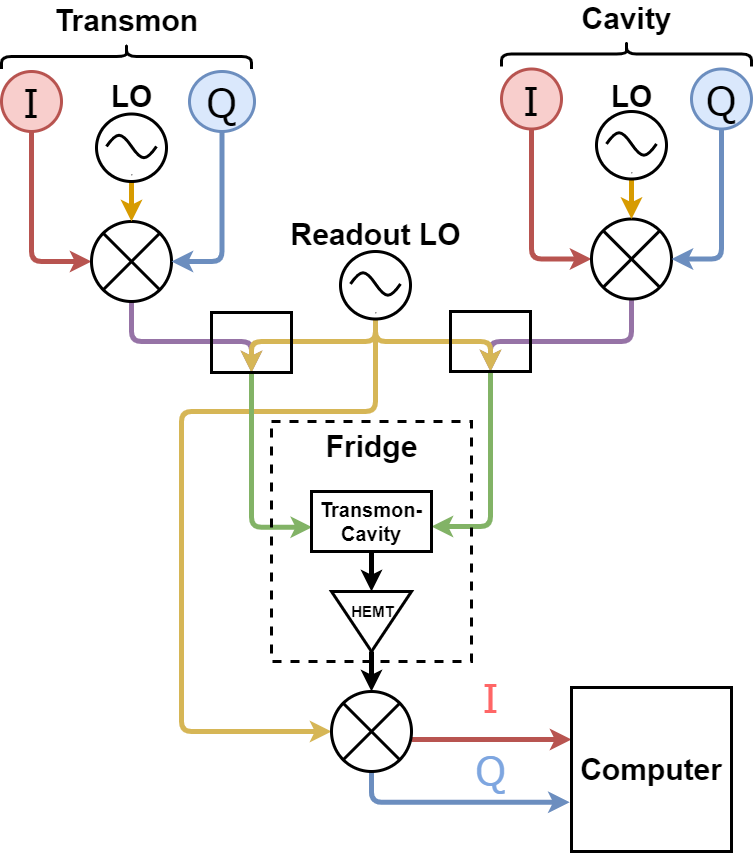
\includegraphics[width=0.85\columnwidth]{gfx/overview.png}
    \caption{Diagram of the system}
    \label{fig:System-diagram}
\end{figure}

The $I$ and $Q$ signals are generated in the AWG, the LO frequency comes from a frequency generator and so does the Read Out signal. \textbf{H}igh \textbf{E}lectron \textbf{M}obility \textbf{T}ransistor (HEMT) is a low-noise cryogenic amplifier.

\section{Generating the Pulses}
\subsection{The AWG}
% It shouldn't be too much of a surprise if I'll tell you that I consider the AWG (Arbitrary Waveform Generator) the "heart\ensuremath\heartsuit" of the system, we've just spent an entire chapter on finding the pulses we want to send, and the instrument that creates and sends the pulse, is the AWG. Unfortunately, using the AWG isn't as straight-forward as you might hope and there are some problem's we'll need to address if we want our system to work.

An \textbf{A}rbitrary \textbf{W}aveform \textbf{G}enerator (AWG) is a device that we use to generate the pulses we calculated with GRAPE in the previous chapter. To control the qubit we need to send RF signals, typically ranging from $4$GHz to $10$GHz. Such signals can be generated by RF signal generators (also called LO's - local oscillators). In contrast, the AWG sends out slowly varying envelopes, usually with a bandwidth of a few hundred MHz. To bridge this gap, we will mix a fixed-frequency signal from the LO with a time-varying signal from the AWG. In particular, this will also enable us to vary the frequency of the LO in real-time with the AWG. Our goal in the next section will be to achieve this so called single-sideband modulation of the LO signal.

We also want to be able to un-mix the measurement result to get back only the interesting parts of the pulse. The device we'll use for this task is the \textit{IQ-Mixer}, but before we can  get into the IQ-Mixer, we need to understand how a \textit{regular} mixer works.

\subsection{The Mixer}
The mixer has 2 inputs and one output. When you enter 2 pulses as an input, you get their product as the output (inputting for example $\cos (t)$ and $\cos (2t)$ will result in $\cos (t)cos (2t)$ at the output).
We draw a mixer in a diagram as
\begin{figure}[H]
    \centering
    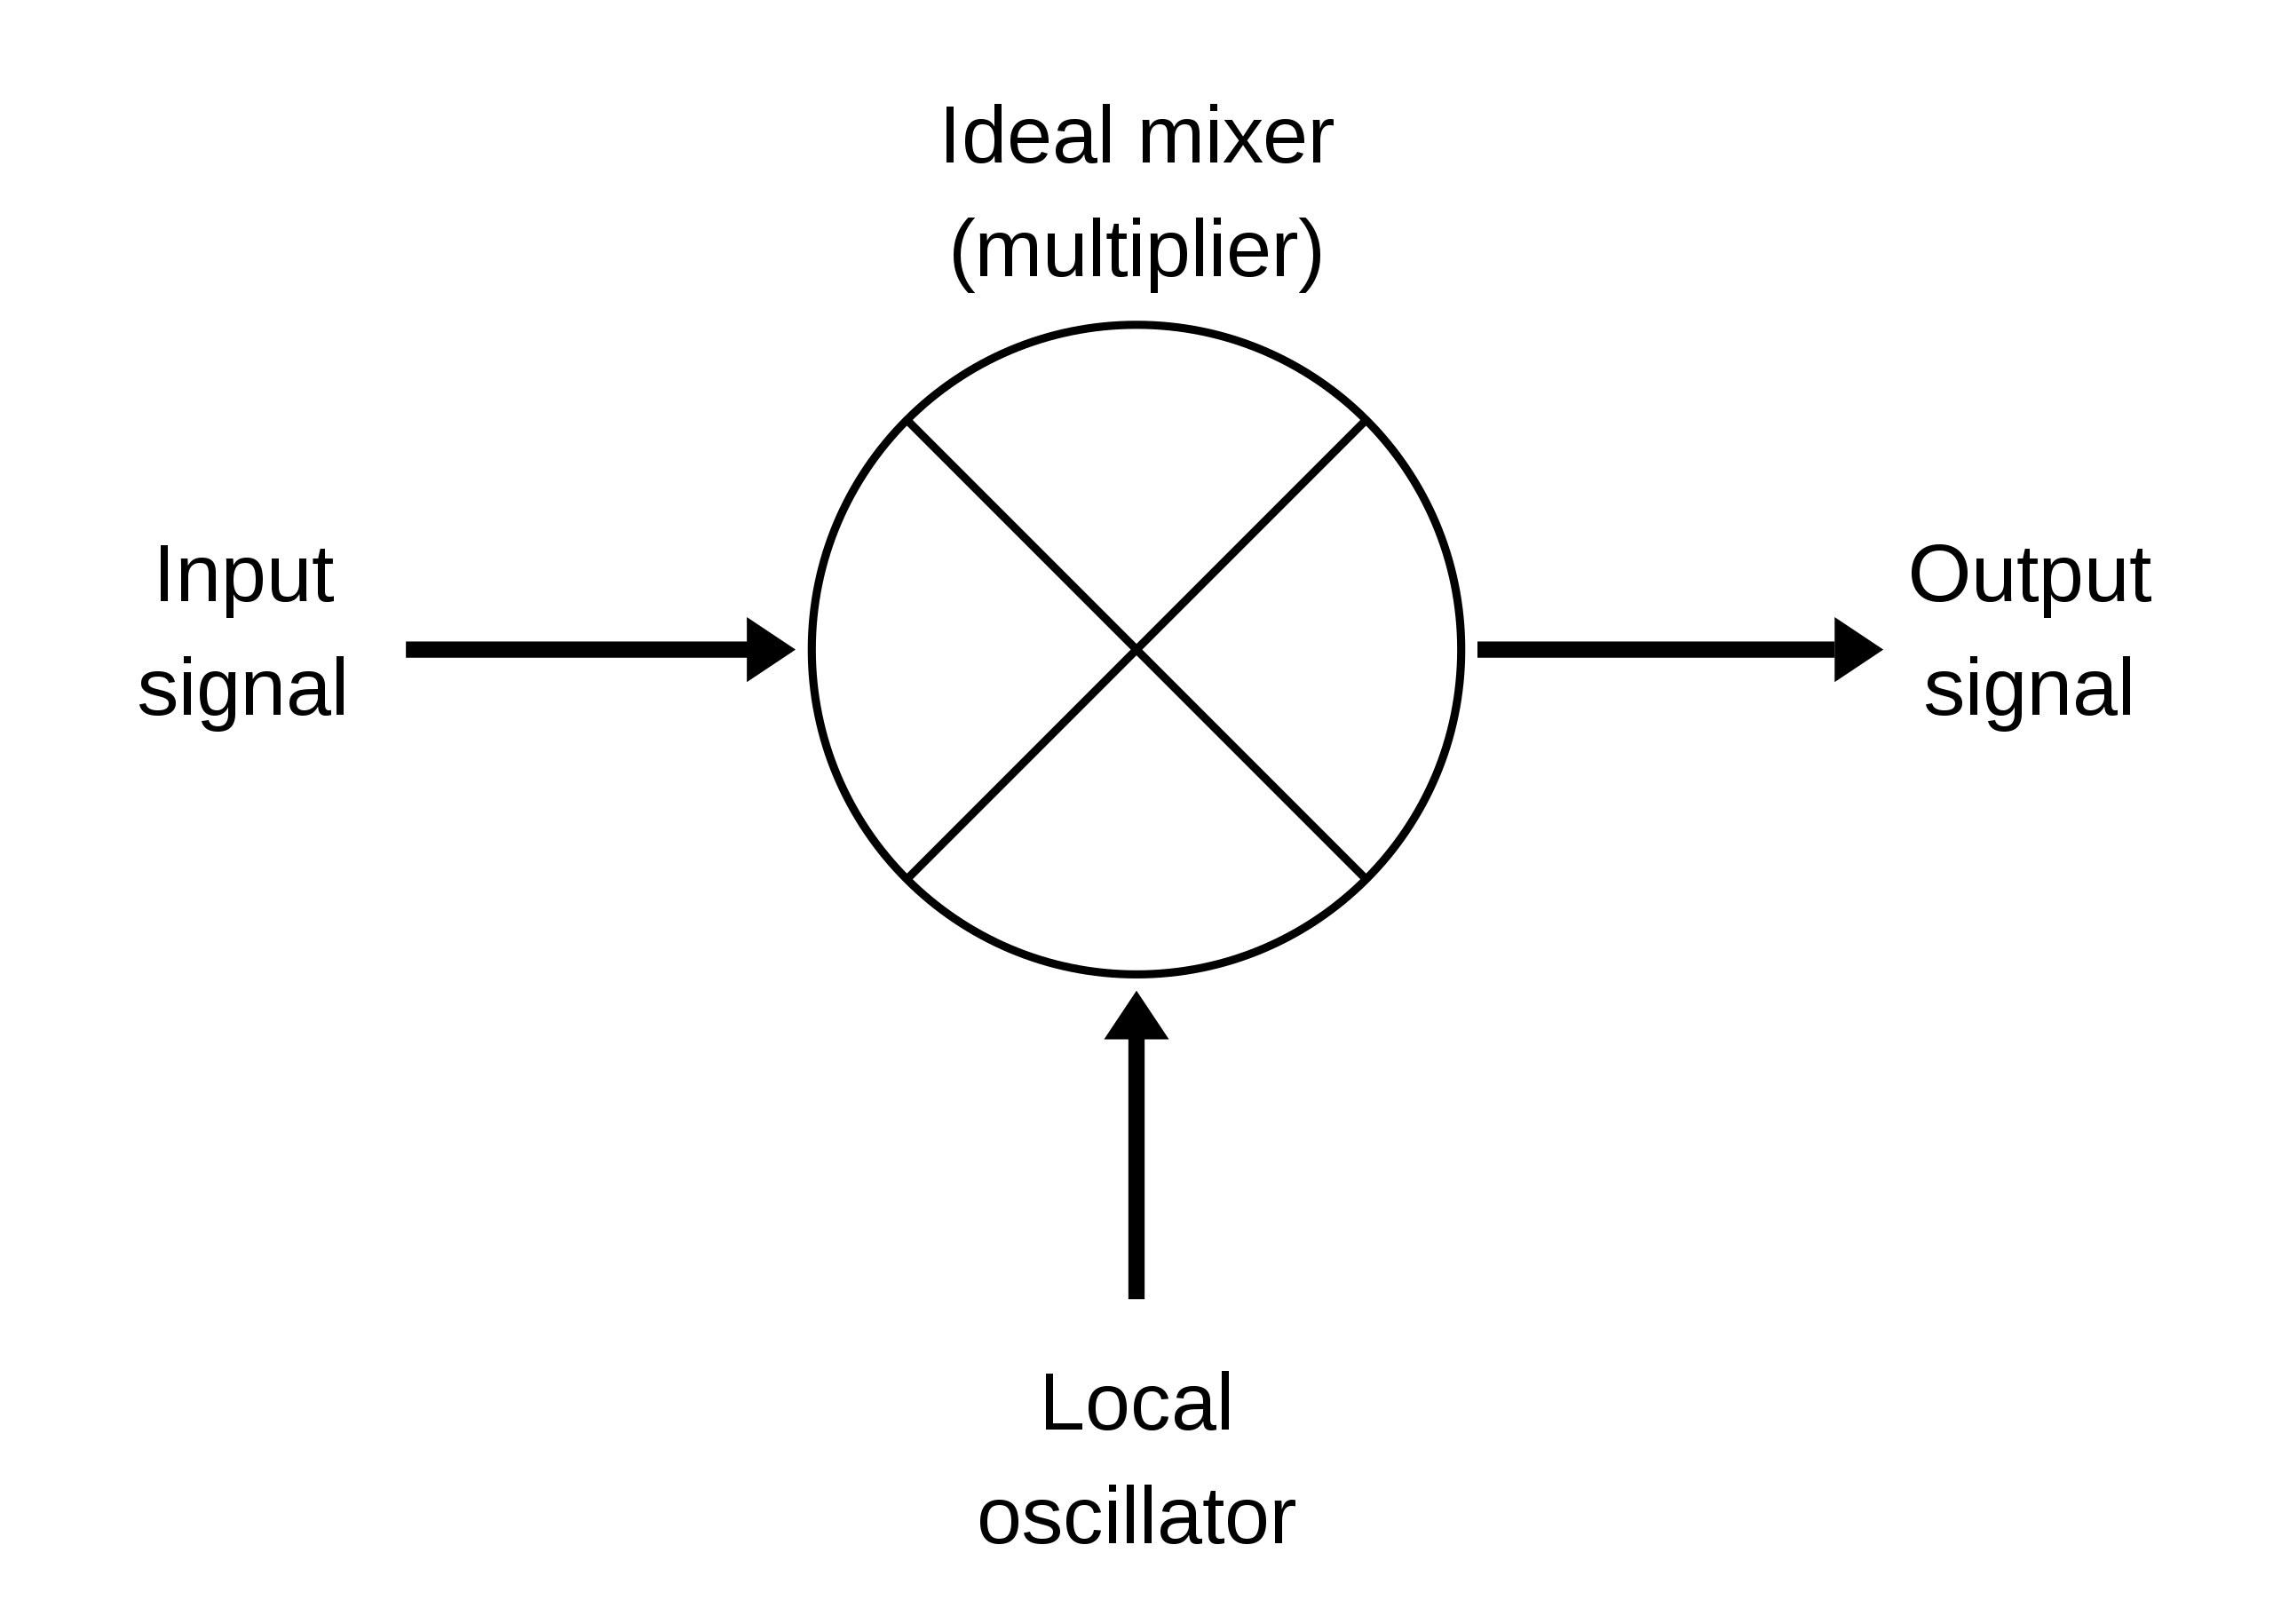
\includegraphics[width=0.5\columnwidth]{gfx/Ideal-Mixer.png}
    \caption{Ideal mixer in a diagram}
    \label{fig:Ideal-Mixer}
\end{figure}
The mixer circuit is \textit{non-linear}. The non-linearity could be achieved with non-linear components, such as diods.
% We can change what are the outputs and what are the inputs to get different ways for the mixer to work\footnote{TODO: Explain this} % TODO: Add on this later

\subsection{The IQ-Mixer}
We've seen what's a \textit{regular} (and \textit{ideal}) mixer is, but how can we use it for the desired effect? remember, we want to input a high frequency and a lower frequency and we want the output to be a wave with a frequency that is the sum of the 2 frequencies. To do so, we can consider the following diagram
\begin{figure}[H]
    \centering
    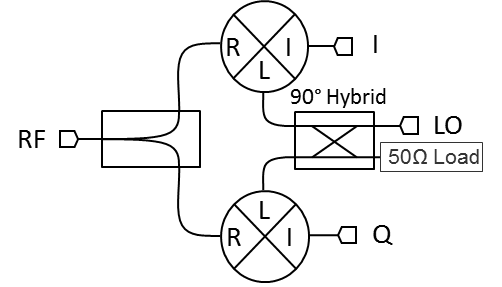
\includegraphics[width=0.5\columnwidth]{gfx/IQ-Mixer.png}
    \caption{The IQ mixer}
    \label{fig:IQ-Mixer}
\end{figure}
Where the 90\degree\ hybrid in the diagram is a \textit{90\degree\  hybrid coupler}. This device splits the signal into 2 signals at a 90\degree phase difference, hence the name. The square near the \textit{RF} sign simply adds the 2 waves.

As we can see, the IQ mixer has 3 inputs, In-phase (\textit{I}), Quadrature (\textit{Q}), hence the name, and \textit{LO}. We can also see that there's only one output, \textit{RF} (although you can reverse the roles of the input and the output).

How can we use this IQ mixer to add frequencies? Let's consider the following inputs\footnote{You can flip I and Q and get subtraction instead of addition}
\begin{align*}
    I &\longrightarrow \cos (\omega_{IQ} t)\\
    Q &\longrightarrow \sin (\omega_{IQ} t)\\
    LO &\longrightarrow \sin (\omega_{LO}t)
\end{align*}
In this case, the input into the top mixer will be \textit{I} and a \textit{LO}, which is $\cos (\omega_{IQ}t)\sin (\omega_{LO}t)$. Similarly, the input into the bottom mixer will be \textit{Q} and 90\degree phase of \textit{LO}, which is $\sin (\omega_{IQ}t)\cos (\omega_{LO}t)$.

The total output (in \textit{RF}) will be the sum of the two waves
$$RF = \cos (\omega_{IQ}t)\sin (\omega_{LO}t) + \sin (\omega_{IQ}t)\cos (\omega_{LO}t)$$
So we get
\begin{equation}
    \boxed{RF = \sin ( (\omega_{LO} + \omega_{IQ})t)}
\end{equation}

Perfect! this is exactly what we wanted, the output is a wave with frequency that is the sum of the input frequencies. Only one problem, this simple scheme turns out not to work in practice : (.

\subsection{Theory VS Reality} \label{sec:solution_real_world} % Maybe combine this section and the next one
If we use a spectrum analyzer and view what frequencies are in the final wave we get the following picture

\begin{figure}[H]
    \centering
    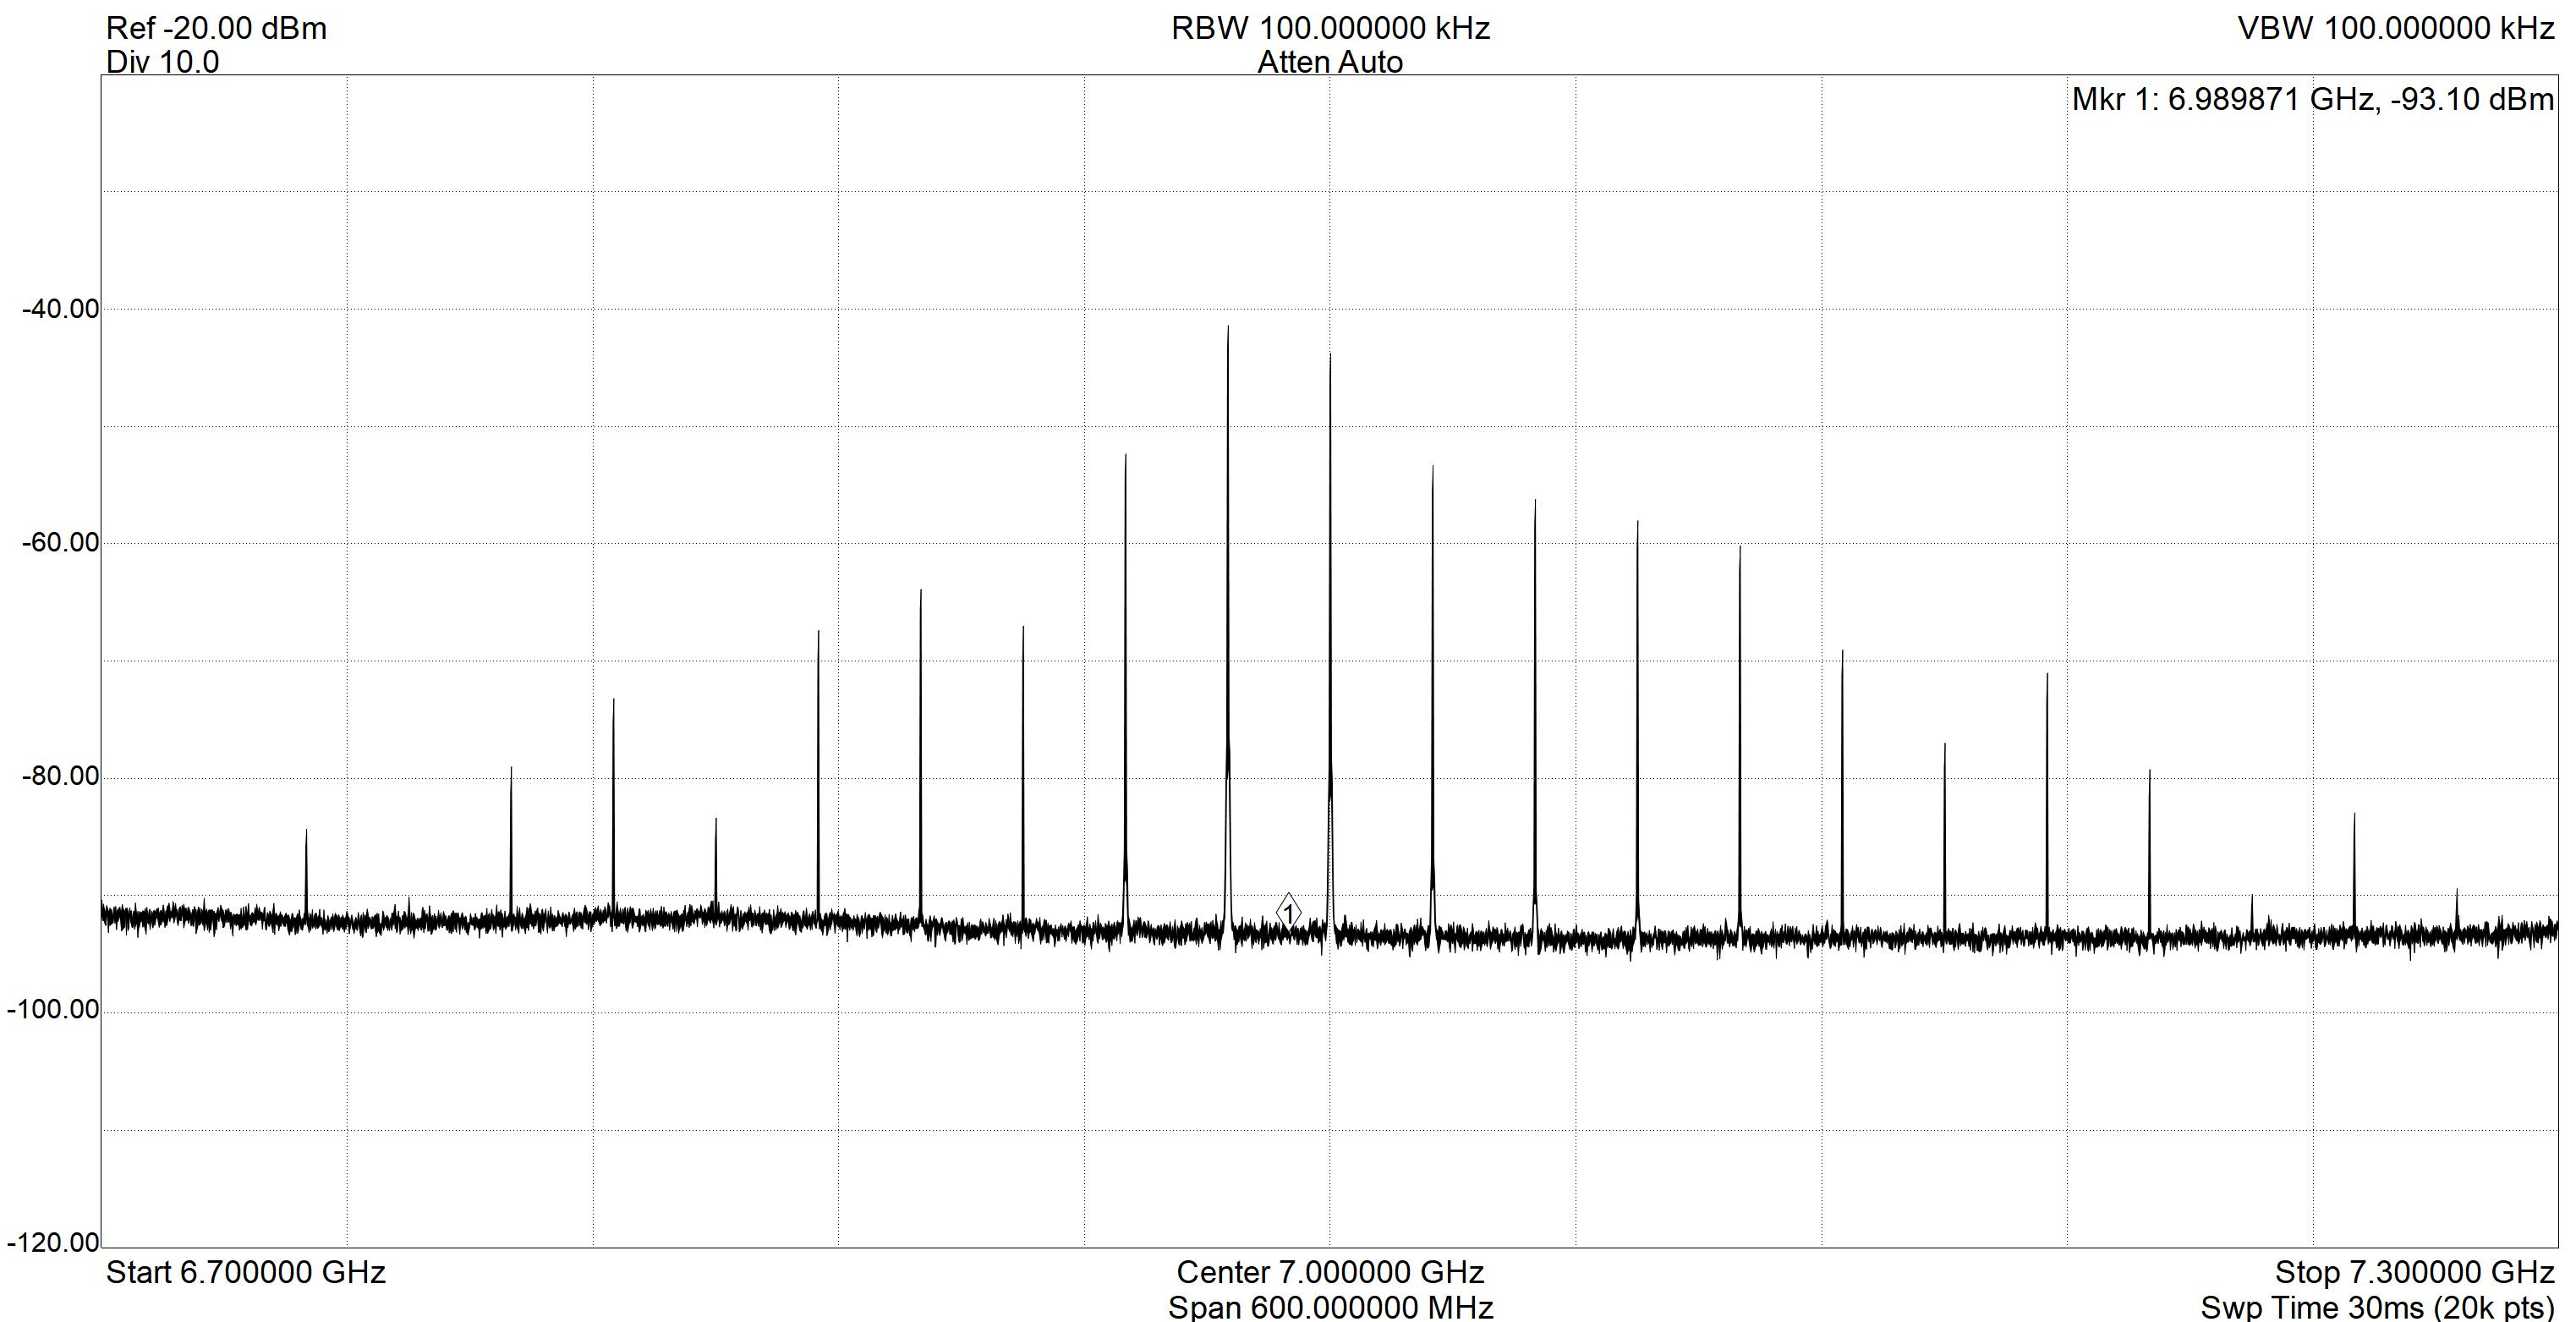
\includegraphics[width=1\columnwidth]{gfx/full-spectrum-no-correction.jpg} %TODO: Need to change to image with explantion on what is going on
    \caption{Full Spectrum Without Any Corrections}
    \label{fig:Full-spectrum-no-corrections}
\end{figure}
Zooming in around the LO frequency we see
% \begin{figure}[H]
%     \centering
%     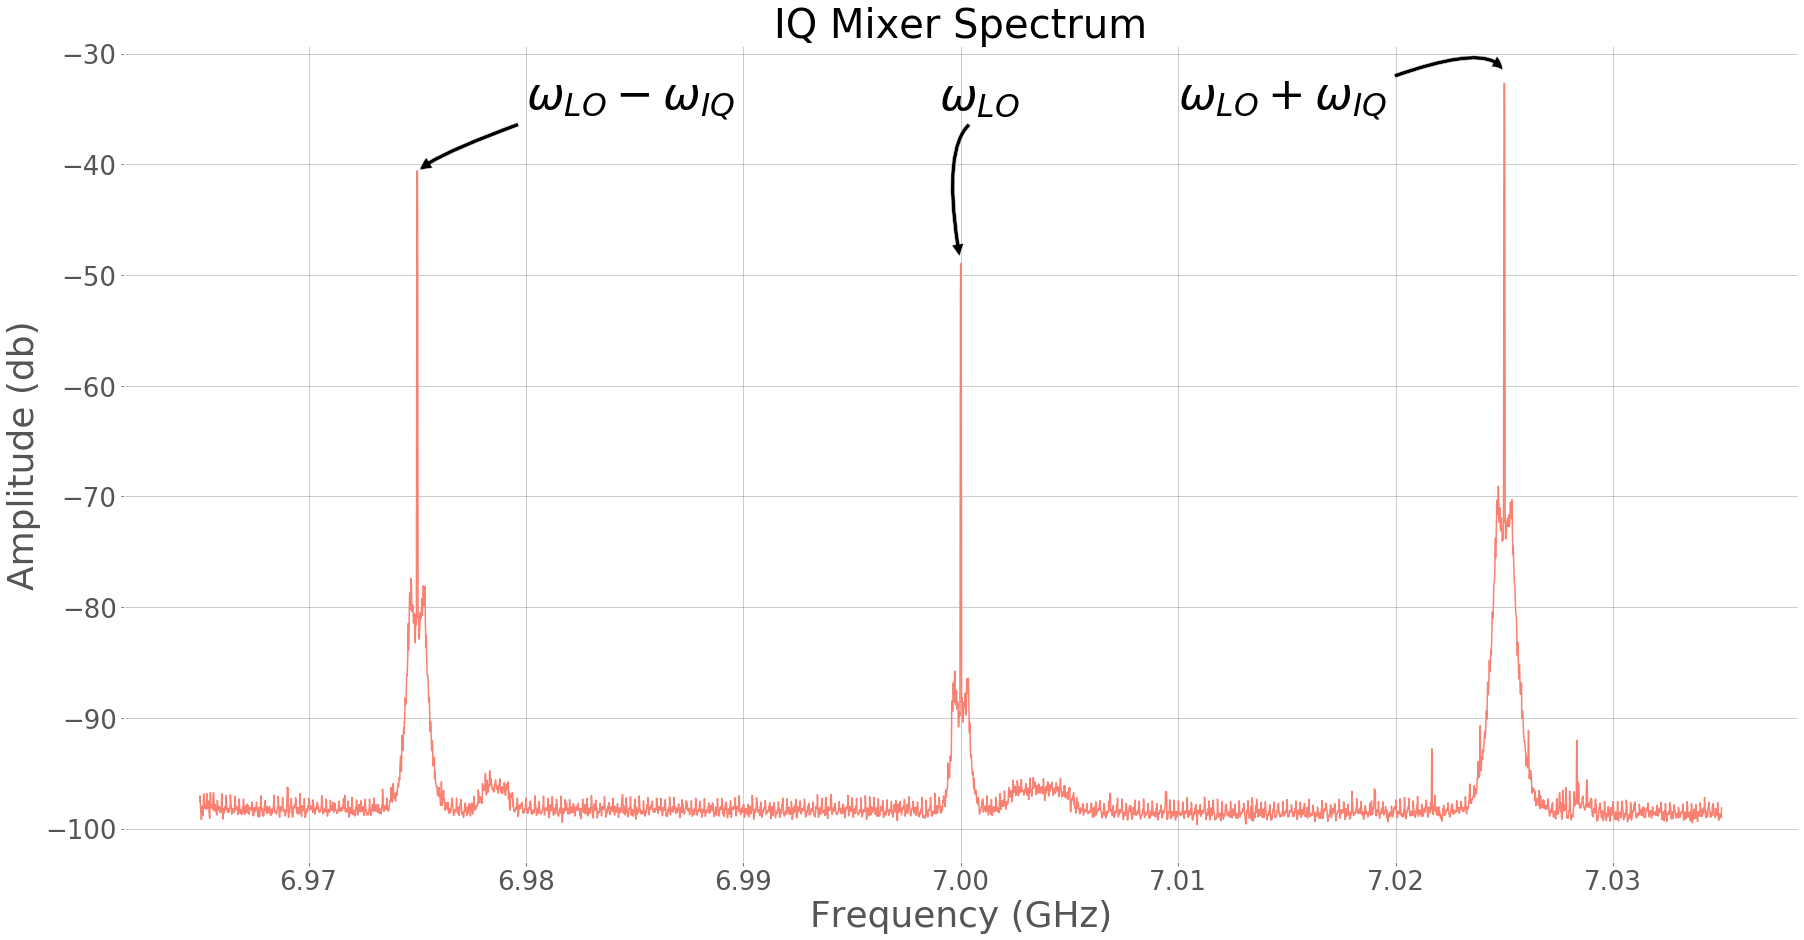
\includegraphics[width=1\columnwidth]{Results/IQ-mixer_before.png} 
%     \caption{Spectrum Around the LO Frequency}
%     \label{fig:closeup-spectrum-no-corrections}
% \end{figure}
\begin{figure}[H]
    \centering
    %% Creator: Matplotlib, PGF backend
%%
%% To include the figure in your LaTeX document, write
%%   \input{<filename>.pgf}
%%
%% Make sure the required packages are loaded in your preamble
%%   \usepackage{pgf}
%%
%% and, on pdftex
%%   \usepackage[utf8]{inputenc}\DeclareUnicodeCharacter{2212}{-}
%%
%% or, on luatex and xetex
%%   \usepackage{unicode-math}
%%
%% Figures using additional raster images can only be included by \input if
%% they are in the same directory as the main LaTeX file. For loading figures
%% from other directories you can use the `import` package
%%   \usepackage{import}
%%
%% and then include the figures with
%%   \import{<path to file>}{<filename>.pgf}
%%
%% Matplotlib used the following preamble
%%
\begingroup%
\makeatletter%
\begin{pgfpicture}%
\pgfpathrectangle{\pgfpointorigin}{\pgfqpoint{4.650000in}{2.400000in}}%
\pgfusepath{use as bounding box, clip}%
\begin{pgfscope}%
\pgfsetbuttcap%
\pgfsetmiterjoin%
\definecolor{currentfill}{rgb}{1.000000,1.000000,1.000000}%
\pgfsetfillcolor{currentfill}%
\pgfsetlinewidth{0.000000pt}%
\definecolor{currentstroke}{rgb}{1.000000,1.000000,1.000000}%
\pgfsetstrokecolor{currentstroke}%
\pgfsetdash{}{0pt}%
\pgfpathmoveto{\pgfqpoint{0.000000in}{0.000000in}}%
\pgfpathlineto{\pgfqpoint{4.650000in}{0.000000in}}%
\pgfpathlineto{\pgfqpoint{4.650000in}{2.400000in}}%
\pgfpathlineto{\pgfqpoint{0.000000in}{2.400000in}}%
\pgfpathclose%
\pgfusepath{fill}%
\end{pgfscope}%
\begin{pgfscope}%
\pgfsetbuttcap%
\pgfsetmiterjoin%
\definecolor{currentfill}{rgb}{1.000000,1.000000,1.000000}%
\pgfsetfillcolor{currentfill}%
\pgfsetlinewidth{0.000000pt}%
\definecolor{currentstroke}{rgb}{0.000000,0.000000,0.000000}%
\pgfsetstrokecolor{currentstroke}%
\pgfsetstrokeopacity{0.000000}%
\pgfsetdash{}{0pt}%
\pgfpathmoveto{\pgfqpoint{0.815516in}{0.604117in}}%
\pgfpathlineto{\pgfqpoint{4.500000in}{0.604117in}}%
\pgfpathlineto{\pgfqpoint{4.500000in}{2.164734in}}%
\pgfpathlineto{\pgfqpoint{0.815516in}{2.164734in}}%
\pgfpathclose%
\pgfusepath{fill}%
\end{pgfscope}%
\begin{pgfscope}%
\pgfpathrectangle{\pgfqpoint{0.815516in}{0.604117in}}{\pgfqpoint{3.684484in}{1.560618in}}%
\pgfusepath{clip}%
\pgfsetrectcap%
\pgfsetroundjoin%
\pgfsetlinewidth{0.803000pt}%
\definecolor{currentstroke}{rgb}{0.501961,0.501961,0.501961}%
\pgfsetstrokecolor{currentstroke}%
\pgfsetstrokeopacity{0.200000}%
\pgfsetdash{}{0pt}%
\pgfpathmoveto{\pgfqpoint{1.461550in}{0.604117in}}%
\pgfpathlineto{\pgfqpoint{1.461550in}{2.164734in}}%
\pgfusepath{stroke}%
\end{pgfscope}%
\begin{pgfscope}%
\pgfsetbuttcap%
\pgfsetroundjoin%
\definecolor{currentfill}{rgb}{0.333333,0.333333,0.333333}%
\pgfsetfillcolor{currentfill}%
\pgfsetlinewidth{0.803000pt}%
\definecolor{currentstroke}{rgb}{0.333333,0.333333,0.333333}%
\pgfsetstrokecolor{currentstroke}%
\pgfsetdash{}{0pt}%
\pgfsys@defobject{currentmarker}{\pgfqpoint{0.000000in}{-0.048611in}}{\pgfqpoint{0.000000in}{0.000000in}}{%
\pgfpathmoveto{\pgfqpoint{0.000000in}{0.000000in}}%
\pgfpathlineto{\pgfqpoint{0.000000in}{-0.048611in}}%
\pgfusepath{stroke,fill}%
}%
\begin{pgfscope}%
\pgfsys@transformshift{1.461550in}{0.604117in}%
\pgfsys@useobject{currentmarker}{}%
\end{pgfscope}%
\end{pgfscope}%
\begin{pgfscope}%
\definecolor{textcolor}{rgb}{0.333333,0.333333,0.333333}%
\pgfsetstrokecolor{textcolor}%
\pgfsetfillcolor{textcolor}%
\pgftext[x=1.461550in,y=0.506895in,,top]{\color{textcolor}\rmfamily\fontsize{11.000000}{13.200000}\selectfont \(\displaystyle {6.975}\)}%
\end{pgfscope}%
\begin{pgfscope}%
\pgfpathrectangle{\pgfqpoint{0.815516in}{0.604117in}}{\pgfqpoint{3.684484in}{1.560618in}}%
\pgfusepath{clip}%
\pgfsetrectcap%
\pgfsetroundjoin%
\pgfsetlinewidth{0.803000pt}%
\definecolor{currentstroke}{rgb}{0.501961,0.501961,0.501961}%
\pgfsetstrokecolor{currentstroke}%
\pgfsetstrokeopacity{0.200000}%
\pgfsetdash{}{0pt}%
\pgfpathmoveto{\pgfqpoint{2.657942in}{0.604117in}}%
\pgfpathlineto{\pgfqpoint{2.657942in}{2.164734in}}%
\pgfusepath{stroke}%
\end{pgfscope}%
\begin{pgfscope}%
\pgfsetbuttcap%
\pgfsetroundjoin%
\definecolor{currentfill}{rgb}{0.333333,0.333333,0.333333}%
\pgfsetfillcolor{currentfill}%
\pgfsetlinewidth{0.803000pt}%
\definecolor{currentstroke}{rgb}{0.333333,0.333333,0.333333}%
\pgfsetstrokecolor{currentstroke}%
\pgfsetdash{}{0pt}%
\pgfsys@defobject{currentmarker}{\pgfqpoint{0.000000in}{-0.048611in}}{\pgfqpoint{0.000000in}{0.000000in}}{%
\pgfpathmoveto{\pgfqpoint{0.000000in}{0.000000in}}%
\pgfpathlineto{\pgfqpoint{0.000000in}{-0.048611in}}%
\pgfusepath{stroke,fill}%
}%
\begin{pgfscope}%
\pgfsys@transformshift{2.657942in}{0.604117in}%
\pgfsys@useobject{currentmarker}{}%
\end{pgfscope}%
\end{pgfscope}%
\begin{pgfscope}%
\definecolor{textcolor}{rgb}{0.333333,0.333333,0.333333}%
\pgfsetstrokecolor{textcolor}%
\pgfsetfillcolor{textcolor}%
\pgftext[x=2.657942in,y=0.506895in,,top]{\color{textcolor}\rmfamily\fontsize{11.000000}{13.200000}\selectfont \(\displaystyle {7.000}\)}%
\end{pgfscope}%
\begin{pgfscope}%
\pgfpathrectangle{\pgfqpoint{0.815516in}{0.604117in}}{\pgfqpoint{3.684484in}{1.560618in}}%
\pgfusepath{clip}%
\pgfsetrectcap%
\pgfsetroundjoin%
\pgfsetlinewidth{0.803000pt}%
\definecolor{currentstroke}{rgb}{0.501961,0.501961,0.501961}%
\pgfsetstrokecolor{currentstroke}%
\pgfsetstrokeopacity{0.200000}%
\pgfsetdash{}{0pt}%
\pgfpathmoveto{\pgfqpoint{3.854335in}{0.604117in}}%
\pgfpathlineto{\pgfqpoint{3.854335in}{2.164734in}}%
\pgfusepath{stroke}%
\end{pgfscope}%
\begin{pgfscope}%
\pgfsetbuttcap%
\pgfsetroundjoin%
\definecolor{currentfill}{rgb}{0.333333,0.333333,0.333333}%
\pgfsetfillcolor{currentfill}%
\pgfsetlinewidth{0.803000pt}%
\definecolor{currentstroke}{rgb}{0.333333,0.333333,0.333333}%
\pgfsetstrokecolor{currentstroke}%
\pgfsetdash{}{0pt}%
\pgfsys@defobject{currentmarker}{\pgfqpoint{0.000000in}{-0.048611in}}{\pgfqpoint{0.000000in}{0.000000in}}{%
\pgfpathmoveto{\pgfqpoint{0.000000in}{0.000000in}}%
\pgfpathlineto{\pgfqpoint{0.000000in}{-0.048611in}}%
\pgfusepath{stroke,fill}%
}%
\begin{pgfscope}%
\pgfsys@transformshift{3.854335in}{0.604117in}%
\pgfsys@useobject{currentmarker}{}%
\end{pgfscope}%
\end{pgfscope}%
\begin{pgfscope}%
\definecolor{textcolor}{rgb}{0.333333,0.333333,0.333333}%
\pgfsetstrokecolor{textcolor}%
\pgfsetfillcolor{textcolor}%
\pgftext[x=3.854335in,y=0.506895in,,top]{\color{textcolor}\rmfamily\fontsize{11.000000}{13.200000}\selectfont \(\displaystyle {7.025}\)}%
\end{pgfscope}%
\begin{pgfscope}%
\definecolor{textcolor}{rgb}{0.333333,0.333333,0.333333}%
\pgfsetstrokecolor{textcolor}%
\pgfsetfillcolor{textcolor}%
\pgftext[x=2.657758in,y=0.316154in,,top]{\color{textcolor}\rmfamily\fontsize{12.000000}{14.400000}\selectfont Frequency (GHz)}%
\end{pgfscope}%
\begin{pgfscope}%
\pgfpathrectangle{\pgfqpoint{0.815516in}{0.604117in}}{\pgfqpoint{3.684484in}{1.560618in}}%
\pgfusepath{clip}%
\pgfsetrectcap%
\pgfsetroundjoin%
\pgfsetlinewidth{0.803000pt}%
\definecolor{currentstroke}{rgb}{0.501961,0.501961,0.501961}%
\pgfsetstrokecolor{currentstroke}%
\pgfsetstrokeopacity{0.200000}%
\pgfsetdash{}{0pt}%
\pgfpathmoveto{\pgfqpoint{0.815516in}{0.667520in}}%
\pgfpathlineto{\pgfqpoint{4.500000in}{0.667520in}}%
\pgfusepath{stroke}%
\end{pgfscope}%
\begin{pgfscope}%
\pgfsetbuttcap%
\pgfsetroundjoin%
\definecolor{currentfill}{rgb}{0.333333,0.333333,0.333333}%
\pgfsetfillcolor{currentfill}%
\pgfsetlinewidth{0.803000pt}%
\definecolor{currentstroke}{rgb}{0.333333,0.333333,0.333333}%
\pgfsetstrokecolor{currentstroke}%
\pgfsetdash{}{0pt}%
\pgfsys@defobject{currentmarker}{\pgfqpoint{-0.048611in}{0.000000in}}{\pgfqpoint{0.000000in}{0.000000in}}{%
\pgfpathmoveto{\pgfqpoint{0.000000in}{0.000000in}}%
\pgfpathlineto{\pgfqpoint{-0.048611in}{0.000000in}}%
\pgfusepath{stroke,fill}%
}%
\begin{pgfscope}%
\pgfsys@transformshift{0.815516in}{0.667520in}%
\pgfsys@useobject{currentmarker}{}%
\end{pgfscope}%
\end{pgfscope}%
\begin{pgfscope}%
\definecolor{textcolor}{rgb}{0.333333,0.333333,0.333333}%
\pgfsetstrokecolor{textcolor}%
\pgfsetfillcolor{textcolor}%
\pgftext[x=0.371882in, y=0.614713in, left, base]{\color{textcolor}\rmfamily\fontsize{11.000000}{13.200000}\selectfont \(\displaystyle {-100}\)}%
\end{pgfscope}%
\begin{pgfscope}%
\pgfpathrectangle{\pgfqpoint{0.815516in}{0.604117in}}{\pgfqpoint{3.684484in}{1.560618in}}%
\pgfusepath{clip}%
\pgfsetrectcap%
\pgfsetroundjoin%
\pgfsetlinewidth{0.803000pt}%
\definecolor{currentstroke}{rgb}{0.501961,0.501961,0.501961}%
\pgfsetstrokecolor{currentstroke}%
\pgfsetstrokeopacity{0.200000}%
\pgfsetdash{}{0pt}%
\pgfpathmoveto{\pgfqpoint{0.815516in}{1.091383in}}%
\pgfpathlineto{\pgfqpoint{4.500000in}{1.091383in}}%
\pgfusepath{stroke}%
\end{pgfscope}%
\begin{pgfscope}%
\pgfsetbuttcap%
\pgfsetroundjoin%
\definecolor{currentfill}{rgb}{0.333333,0.333333,0.333333}%
\pgfsetfillcolor{currentfill}%
\pgfsetlinewidth{0.803000pt}%
\definecolor{currentstroke}{rgb}{0.333333,0.333333,0.333333}%
\pgfsetstrokecolor{currentstroke}%
\pgfsetdash{}{0pt}%
\pgfsys@defobject{currentmarker}{\pgfqpoint{-0.048611in}{0.000000in}}{\pgfqpoint{0.000000in}{0.000000in}}{%
\pgfpathmoveto{\pgfqpoint{0.000000in}{0.000000in}}%
\pgfpathlineto{\pgfqpoint{-0.048611in}{0.000000in}}%
\pgfusepath{stroke,fill}%
}%
\begin{pgfscope}%
\pgfsys@transformshift{0.815516in}{1.091383in}%
\pgfsys@useobject{currentmarker}{}%
\end{pgfscope}%
\end{pgfscope}%
\begin{pgfscope}%
\definecolor{textcolor}{rgb}{0.333333,0.333333,0.333333}%
\pgfsetstrokecolor{textcolor}%
\pgfsetfillcolor{textcolor}%
\pgftext[x=0.447923in, y=1.038577in, left, base]{\color{textcolor}\rmfamily\fontsize{11.000000}{13.200000}\selectfont \(\displaystyle {-80}\)}%
\end{pgfscope}%
\begin{pgfscope}%
\pgfpathrectangle{\pgfqpoint{0.815516in}{0.604117in}}{\pgfqpoint{3.684484in}{1.560618in}}%
\pgfusepath{clip}%
\pgfsetrectcap%
\pgfsetroundjoin%
\pgfsetlinewidth{0.803000pt}%
\definecolor{currentstroke}{rgb}{0.501961,0.501961,0.501961}%
\pgfsetstrokecolor{currentstroke}%
\pgfsetstrokeopacity{0.200000}%
\pgfsetdash{}{0pt}%
\pgfpathmoveto{\pgfqpoint{0.815516in}{1.515247in}}%
\pgfpathlineto{\pgfqpoint{4.500000in}{1.515247in}}%
\pgfusepath{stroke}%
\end{pgfscope}%
\begin{pgfscope}%
\pgfsetbuttcap%
\pgfsetroundjoin%
\definecolor{currentfill}{rgb}{0.333333,0.333333,0.333333}%
\pgfsetfillcolor{currentfill}%
\pgfsetlinewidth{0.803000pt}%
\definecolor{currentstroke}{rgb}{0.333333,0.333333,0.333333}%
\pgfsetstrokecolor{currentstroke}%
\pgfsetdash{}{0pt}%
\pgfsys@defobject{currentmarker}{\pgfqpoint{-0.048611in}{0.000000in}}{\pgfqpoint{0.000000in}{0.000000in}}{%
\pgfpathmoveto{\pgfqpoint{0.000000in}{0.000000in}}%
\pgfpathlineto{\pgfqpoint{-0.048611in}{0.000000in}}%
\pgfusepath{stroke,fill}%
}%
\begin{pgfscope}%
\pgfsys@transformshift{0.815516in}{1.515247in}%
\pgfsys@useobject{currentmarker}{}%
\end{pgfscope}%
\end{pgfscope}%
\begin{pgfscope}%
\definecolor{textcolor}{rgb}{0.333333,0.333333,0.333333}%
\pgfsetstrokecolor{textcolor}%
\pgfsetfillcolor{textcolor}%
\pgftext[x=0.447923in, y=1.462440in, left, base]{\color{textcolor}\rmfamily\fontsize{11.000000}{13.200000}\selectfont \(\displaystyle {-60}\)}%
\end{pgfscope}%
\begin{pgfscope}%
\pgfpathrectangle{\pgfqpoint{0.815516in}{0.604117in}}{\pgfqpoint{3.684484in}{1.560618in}}%
\pgfusepath{clip}%
\pgfsetrectcap%
\pgfsetroundjoin%
\pgfsetlinewidth{0.803000pt}%
\definecolor{currentstroke}{rgb}{0.501961,0.501961,0.501961}%
\pgfsetstrokecolor{currentstroke}%
\pgfsetstrokeopacity{0.200000}%
\pgfsetdash{}{0pt}%
\pgfpathmoveto{\pgfqpoint{0.815516in}{1.939110in}}%
\pgfpathlineto{\pgfqpoint{4.500000in}{1.939110in}}%
\pgfusepath{stroke}%
\end{pgfscope}%
\begin{pgfscope}%
\pgfsetbuttcap%
\pgfsetroundjoin%
\definecolor{currentfill}{rgb}{0.333333,0.333333,0.333333}%
\pgfsetfillcolor{currentfill}%
\pgfsetlinewidth{0.803000pt}%
\definecolor{currentstroke}{rgb}{0.333333,0.333333,0.333333}%
\pgfsetstrokecolor{currentstroke}%
\pgfsetdash{}{0pt}%
\pgfsys@defobject{currentmarker}{\pgfqpoint{-0.048611in}{0.000000in}}{\pgfqpoint{0.000000in}{0.000000in}}{%
\pgfpathmoveto{\pgfqpoint{0.000000in}{0.000000in}}%
\pgfpathlineto{\pgfqpoint{-0.048611in}{0.000000in}}%
\pgfusepath{stroke,fill}%
}%
\begin{pgfscope}%
\pgfsys@transformshift{0.815516in}{1.939110in}%
\pgfsys@useobject{currentmarker}{}%
\end{pgfscope}%
\end{pgfscope}%
\begin{pgfscope}%
\definecolor{textcolor}{rgb}{0.333333,0.333333,0.333333}%
\pgfsetstrokecolor{textcolor}%
\pgfsetfillcolor{textcolor}%
\pgftext[x=0.447923in, y=1.886304in, left, base]{\color{textcolor}\rmfamily\fontsize{11.000000}{13.200000}\selectfont \(\displaystyle {-40}\)}%
\end{pgfscope}%
\begin{pgfscope}%
\definecolor{textcolor}{rgb}{0.333333,0.333333,0.333333}%
\pgfsetstrokecolor{textcolor}%
\pgfsetfillcolor{textcolor}%
\pgftext[x=0.316326in,y=1.384426in,,bottom,rotate=90.000000]{\color{textcolor}\rmfamily\fontsize{12.000000}{14.400000}\selectfont Amplitude (db)}%
\end{pgfscope}%
\begin{pgfscope}%
\pgfpathrectangle{\pgfqpoint{0.815516in}{0.604117in}}{\pgfqpoint{3.684484in}{1.560618in}}%
\pgfusepath{clip}%
\pgfsetrectcap%
\pgfsetroundjoin%
\pgfsetlinewidth{1.003750pt}%
\definecolor{currentstroke}{rgb}{0.886275,0.290196,0.200000}%
\pgfsetstrokecolor{currentstroke}%
\pgfsetdash{}{0pt}%
\pgfpathmoveto{\pgfqpoint{0.982993in}{0.720975in}}%
\pgfpathlineto{\pgfqpoint{0.983361in}{0.730341in}}%
\pgfpathlineto{\pgfqpoint{0.984097in}{0.715910in}}%
\pgfpathlineto{\pgfqpoint{0.986674in}{0.685055in}}%
\pgfpathlineto{\pgfqpoint{0.987042in}{0.689058in}}%
\pgfpathlineto{\pgfqpoint{0.988515in}{0.710856in}}%
\pgfpathlineto{\pgfqpoint{0.988883in}{0.706657in}}%
\pgfpathlineto{\pgfqpoint{0.989987in}{0.692937in}}%
\pgfpathlineto{\pgfqpoint{0.990355in}{0.696590in}}%
\pgfpathlineto{\pgfqpoint{0.991828in}{0.734041in}}%
\pgfpathlineto{\pgfqpoint{0.992932in}{0.726375in}}%
\pgfpathlineto{\pgfqpoint{0.994773in}{0.706053in}}%
\pgfpathlineto{\pgfqpoint{0.996613in}{0.707221in}}%
\pgfpathlineto{\pgfqpoint{0.997718in}{0.705034in}}%
\pgfpathlineto{\pgfqpoint{0.998822in}{0.734520in}}%
\pgfpathlineto{\pgfqpoint{0.999558in}{0.722050in}}%
\pgfpathlineto{\pgfqpoint{1.000295in}{0.706971in}}%
\pgfpathlineto{\pgfqpoint{1.001031in}{0.716974in}}%
\pgfpathlineto{\pgfqpoint{1.001767in}{0.720462in}}%
\pgfpathlineto{\pgfqpoint{1.002135in}{0.713653in}}%
\pgfpathlineto{\pgfqpoint{1.002503in}{0.719339in}}%
\pgfpathlineto{\pgfqpoint{1.004712in}{0.687537in}}%
\pgfpathlineto{\pgfqpoint{1.006184in}{0.736652in}}%
\pgfpathlineto{\pgfqpoint{1.006921in}{0.722387in}}%
\pgfpathlineto{\pgfqpoint{1.007657in}{0.707829in}}%
\pgfpathlineto{\pgfqpoint{1.008761in}{0.710423in}}%
\pgfpathlineto{\pgfqpoint{1.009129in}{0.712049in}}%
\pgfpathlineto{\pgfqpoint{1.009866in}{0.710345in}}%
\pgfpathlineto{\pgfqpoint{1.010970in}{0.706034in}}%
\pgfpathlineto{\pgfqpoint{1.011338in}{0.704277in}}%
\pgfpathlineto{\pgfqpoint{1.012811in}{0.736317in}}%
\pgfpathlineto{\pgfqpoint{1.013547in}{0.735970in}}%
\pgfpathlineto{\pgfqpoint{1.015756in}{0.700842in}}%
\pgfpathlineto{\pgfqpoint{1.016124in}{0.704339in}}%
\pgfpathlineto{\pgfqpoint{1.016860in}{0.713666in}}%
\pgfpathlineto{\pgfqpoint{1.017596in}{0.709542in}}%
\pgfpathlineto{\pgfqpoint{1.020541in}{0.693693in}}%
\pgfpathlineto{\pgfqpoint{1.020909in}{0.693895in}}%
\pgfpathlineto{\pgfqpoint{1.021646in}{0.721581in}}%
\pgfpathlineto{\pgfqpoint{1.022750in}{0.711890in}}%
\pgfpathlineto{\pgfqpoint{1.024959in}{0.703360in}}%
\pgfpathlineto{\pgfqpoint{1.025327in}{0.703425in}}%
\pgfpathlineto{\pgfqpoint{1.026063in}{0.709726in}}%
\pgfpathlineto{\pgfqpoint{1.026799in}{0.703637in}}%
\pgfpathlineto{\pgfqpoint{1.027167in}{0.698892in}}%
\pgfpathlineto{\pgfqpoint{1.027904in}{0.704152in}}%
\pgfpathlineto{\pgfqpoint{1.028640in}{0.706628in}}%
\pgfpathlineto{\pgfqpoint{1.029008in}{0.702419in}}%
\pgfpathlineto{\pgfqpoint{1.029376in}{0.698968in}}%
\pgfpathlineto{\pgfqpoint{1.030112in}{0.704205in}}%
\pgfpathlineto{\pgfqpoint{1.030849in}{0.713903in}}%
\pgfpathlineto{\pgfqpoint{1.031217in}{0.734357in}}%
\pgfpathlineto{\pgfqpoint{1.032321in}{0.711877in}}%
\pgfpathlineto{\pgfqpoint{1.033794in}{0.685814in}}%
\pgfpathlineto{\pgfqpoint{1.034530in}{0.691771in}}%
\pgfpathlineto{\pgfqpoint{1.035634in}{0.706115in}}%
\pgfpathlineto{\pgfqpoint{1.036370in}{0.700668in}}%
\pgfpathlineto{\pgfqpoint{1.036739in}{0.697517in}}%
\pgfpathlineto{\pgfqpoint{1.037475in}{0.701353in}}%
\pgfpathlineto{\pgfqpoint{1.038211in}{0.709724in}}%
\pgfpathlineto{\pgfqpoint{1.039315in}{0.705468in}}%
\pgfpathlineto{\pgfqpoint{1.039683in}{0.703519in}}%
\pgfpathlineto{\pgfqpoint{1.040052in}{0.706149in}}%
\pgfpathlineto{\pgfqpoint{1.040788in}{0.730625in}}%
\pgfpathlineto{\pgfqpoint{1.041892in}{0.716915in}}%
\pgfpathlineto{\pgfqpoint{1.044837in}{0.698462in}}%
\pgfpathlineto{\pgfqpoint{1.045942in}{0.705809in}}%
\pgfpathlineto{\pgfqpoint{1.046678in}{0.701109in}}%
\pgfpathlineto{\pgfqpoint{1.047046in}{0.699901in}}%
\pgfpathlineto{\pgfqpoint{1.047782in}{0.701124in}}%
\pgfpathlineto{\pgfqpoint{1.049991in}{0.719405in}}%
\pgfpathlineto{\pgfqpoint{1.050359in}{0.732329in}}%
\pgfpathlineto{\pgfqpoint{1.051463in}{0.717336in}}%
\pgfpathlineto{\pgfqpoint{1.053672in}{0.695255in}}%
\pgfpathlineto{\pgfqpoint{1.054408in}{0.700886in}}%
\pgfpathlineto{\pgfqpoint{1.055145in}{0.706452in}}%
\pgfpathlineto{\pgfqpoint{1.056249in}{0.705203in}}%
\pgfpathlineto{\pgfqpoint{1.056617in}{0.704843in}}%
\pgfpathlineto{\pgfqpoint{1.057721in}{0.698288in}}%
\pgfpathlineto{\pgfqpoint{1.058090in}{0.700954in}}%
\pgfpathlineto{\pgfqpoint{1.059562in}{0.712774in}}%
\pgfpathlineto{\pgfqpoint{1.059930in}{0.729374in}}%
\pgfpathlineto{\pgfqpoint{1.061034in}{0.714791in}}%
\pgfpathlineto{\pgfqpoint{1.061771in}{0.703251in}}%
\pgfpathlineto{\pgfqpoint{1.062875in}{0.707744in}}%
\pgfpathlineto{\pgfqpoint{1.063979in}{0.710639in}}%
\pgfpathlineto{\pgfqpoint{1.064716in}{0.708916in}}%
\pgfpathlineto{\pgfqpoint{1.066924in}{0.694670in}}%
\pgfpathlineto{\pgfqpoint{1.067293in}{0.695488in}}%
\pgfpathlineto{\pgfqpoint{1.069501in}{0.724561in}}%
\pgfpathlineto{\pgfqpoint{1.070238in}{0.716135in}}%
\pgfpathlineto{\pgfqpoint{1.072078in}{0.697063in}}%
\pgfpathlineto{\pgfqpoint{1.072446in}{0.697267in}}%
\pgfpathlineto{\pgfqpoint{1.073919in}{0.703374in}}%
\pgfpathlineto{\pgfqpoint{1.074287in}{0.700431in}}%
\pgfpathlineto{\pgfqpoint{1.075023in}{0.694452in}}%
\pgfpathlineto{\pgfqpoint{1.075759in}{0.696050in}}%
\pgfpathlineto{\pgfqpoint{1.076496in}{0.701548in}}%
\pgfpathlineto{\pgfqpoint{1.077232in}{0.709866in}}%
\pgfpathlineto{\pgfqpoint{1.077968in}{0.702662in}}%
\pgfpathlineto{\pgfqpoint{1.078336in}{0.699502in}}%
\pgfpathlineto{\pgfqpoint{1.079072in}{0.724468in}}%
\pgfpathlineto{\pgfqpoint{1.080177in}{0.710243in}}%
\pgfpathlineto{\pgfqpoint{1.081281in}{0.694554in}}%
\pgfpathlineto{\pgfqpoint{1.082017in}{0.698780in}}%
\pgfpathlineto{\pgfqpoint{1.083490in}{0.710868in}}%
\pgfpathlineto{\pgfqpoint{1.084226in}{0.706564in}}%
\pgfpathlineto{\pgfqpoint{1.084962in}{0.697981in}}%
\pgfpathlineto{\pgfqpoint{1.085699in}{0.700056in}}%
\pgfpathlineto{\pgfqpoint{1.087171in}{0.714357in}}%
\pgfpathlineto{\pgfqpoint{1.087907in}{0.708387in}}%
\pgfpathlineto{\pgfqpoint{1.088275in}{0.698345in}}%
\pgfpathlineto{\pgfqpoint{1.088644in}{0.712492in}}%
\pgfpathlineto{\pgfqpoint{1.089380in}{0.709525in}}%
\pgfpathlineto{\pgfqpoint{1.091589in}{0.695262in}}%
\pgfpathlineto{\pgfqpoint{1.092325in}{0.699221in}}%
\pgfpathlineto{\pgfqpoint{1.093797in}{0.708435in}}%
\pgfpathlineto{\pgfqpoint{1.094165in}{0.707251in}}%
\pgfpathlineto{\pgfqpoint{1.094902in}{0.708007in}}%
\pgfpathlineto{\pgfqpoint{1.095638in}{0.706666in}}%
\pgfpathlineto{\pgfqpoint{1.096006in}{0.707187in}}%
\pgfpathlineto{\pgfqpoint{1.096374in}{0.705087in}}%
\pgfpathlineto{\pgfqpoint{1.096742in}{0.703478in}}%
\pgfpathlineto{\pgfqpoint{1.097110in}{0.705254in}}%
\pgfpathlineto{\pgfqpoint{1.098215in}{0.718468in}}%
\pgfpathlineto{\pgfqpoint{1.097847in}{0.703158in}}%
\pgfpathlineto{\pgfqpoint{1.098951in}{0.712114in}}%
\pgfpathlineto{\pgfqpoint{1.100423in}{0.692581in}}%
\pgfpathlineto{\pgfqpoint{1.101160in}{0.692998in}}%
\pgfpathlineto{\pgfqpoint{1.101528in}{0.692420in}}%
\pgfpathlineto{\pgfqpoint{1.101896in}{0.694689in}}%
\pgfpathlineto{\pgfqpoint{1.103000in}{0.707346in}}%
\pgfpathlineto{\pgfqpoint{1.103368in}{0.703792in}}%
\pgfpathlineto{\pgfqpoint{1.104105in}{0.699072in}}%
\pgfpathlineto{\pgfqpoint{1.104473in}{0.704080in}}%
\pgfpathlineto{\pgfqpoint{1.106313in}{0.707605in}}%
\pgfpathlineto{\pgfqpoint{1.106681in}{0.708700in}}%
\pgfpathlineto{\pgfqpoint{1.107050in}{0.706295in}}%
\pgfpathlineto{\pgfqpoint{1.107418in}{0.706598in}}%
\pgfpathlineto{\pgfqpoint{1.107786in}{0.718396in}}%
\pgfpathlineto{\pgfqpoint{1.108522in}{0.706197in}}%
\pgfpathlineto{\pgfqpoint{1.111099in}{0.691140in}}%
\pgfpathlineto{\pgfqpoint{1.112571in}{0.708132in}}%
\pgfpathlineto{\pgfqpoint{1.112940in}{0.705676in}}%
\pgfpathlineto{\pgfqpoint{1.114412in}{0.689440in}}%
\pgfpathlineto{\pgfqpoint{1.114780in}{0.692778in}}%
\pgfpathlineto{\pgfqpoint{1.117357in}{0.730569in}}%
\pgfpathlineto{\pgfqpoint{1.117725in}{0.721990in}}%
\pgfpathlineto{\pgfqpoint{1.119198in}{0.701753in}}%
\pgfpathlineto{\pgfqpoint{1.119934in}{0.705212in}}%
\pgfpathlineto{\pgfqpoint{1.120302in}{0.705888in}}%
\pgfpathlineto{\pgfqpoint{1.123247in}{0.691892in}}%
\pgfpathlineto{\pgfqpoint{1.123615in}{0.691816in}}%
\pgfpathlineto{\pgfqpoint{1.126192in}{0.713431in}}%
\pgfpathlineto{\pgfqpoint{1.126560in}{0.703819in}}%
\pgfpathlineto{\pgfqpoint{1.126928in}{0.721247in}}%
\pgfpathlineto{\pgfqpoint{1.128032in}{0.704167in}}%
\pgfpathlineto{\pgfqpoint{1.128401in}{0.702607in}}%
\pgfpathlineto{\pgfqpoint{1.128769in}{0.705689in}}%
\pgfpathlineto{\pgfqpoint{1.129137in}{0.707285in}}%
\pgfpathlineto{\pgfqpoint{1.129505in}{0.703182in}}%
\pgfpathlineto{\pgfqpoint{1.130241in}{0.696260in}}%
\pgfpathlineto{\pgfqpoint{1.130977in}{0.702859in}}%
\pgfpathlineto{\pgfqpoint{1.131714in}{0.710483in}}%
\pgfpathlineto{\pgfqpoint{1.132450in}{0.704849in}}%
\pgfpathlineto{\pgfqpoint{1.135763in}{0.697612in}}%
\pgfpathlineto{\pgfqpoint{1.136499in}{0.710192in}}%
\pgfpathlineto{\pgfqpoint{1.137235in}{0.702503in}}%
\pgfpathlineto{\pgfqpoint{1.139812in}{0.693022in}}%
\pgfpathlineto{\pgfqpoint{1.140180in}{0.694183in}}%
\pgfpathlineto{\pgfqpoint{1.141285in}{0.705011in}}%
\pgfpathlineto{\pgfqpoint{1.141653in}{0.702671in}}%
\pgfpathlineto{\pgfqpoint{1.142389in}{0.696018in}}%
\pgfpathlineto{\pgfqpoint{1.143125in}{0.700486in}}%
\pgfpathlineto{\pgfqpoint{1.145702in}{0.718633in}}%
\pgfpathlineto{\pgfqpoint{1.146070in}{0.731506in}}%
\pgfpathlineto{\pgfqpoint{1.146807in}{0.715270in}}%
\pgfpathlineto{\pgfqpoint{1.148279in}{0.698712in}}%
\pgfpathlineto{\pgfqpoint{1.149015in}{0.700162in}}%
\pgfpathlineto{\pgfqpoint{1.149383in}{0.701603in}}%
\pgfpathlineto{\pgfqpoint{1.150120in}{0.699333in}}%
\pgfpathlineto{\pgfqpoint{1.151224in}{0.698366in}}%
\pgfpathlineto{\pgfqpoint{1.151960in}{0.695618in}}%
\pgfpathlineto{\pgfqpoint{1.152328in}{0.696991in}}%
\pgfpathlineto{\pgfqpoint{1.155273in}{0.712659in}}%
\pgfpathlineto{\pgfqpoint{1.155642in}{0.729436in}}%
\pgfpathlineto{\pgfqpoint{1.156378in}{0.716720in}}%
\pgfpathlineto{\pgfqpoint{1.158587in}{0.689442in}}%
\pgfpathlineto{\pgfqpoint{1.158955in}{0.689629in}}%
\pgfpathlineto{\pgfqpoint{1.160427in}{0.709629in}}%
\pgfpathlineto{\pgfqpoint{1.161163in}{0.704862in}}%
\pgfpathlineto{\pgfqpoint{1.162636in}{0.700382in}}%
\pgfpathlineto{\pgfqpoint{1.163372in}{0.703360in}}%
\pgfpathlineto{\pgfqpoint{1.165213in}{0.726835in}}%
\pgfpathlineto{\pgfqpoint{1.165581in}{0.718224in}}%
\pgfpathlineto{\pgfqpoint{1.167789in}{0.700619in}}%
\pgfpathlineto{\pgfqpoint{1.168158in}{0.699962in}}%
\pgfpathlineto{\pgfqpoint{1.168894in}{0.701467in}}%
\pgfpathlineto{\pgfqpoint{1.169630in}{0.704002in}}%
\pgfpathlineto{\pgfqpoint{1.169998in}{0.702147in}}%
\pgfpathlineto{\pgfqpoint{1.171103in}{0.691544in}}%
\pgfpathlineto{\pgfqpoint{1.171839in}{0.693831in}}%
\pgfpathlineto{\pgfqpoint{1.175152in}{0.725218in}}%
\pgfpathlineto{\pgfqpoint{1.175520in}{0.746977in}}%
\pgfpathlineto{\pgfqpoint{1.176993in}{0.743006in}}%
\pgfpathlineto{\pgfqpoint{1.177361in}{0.745371in}}%
\pgfpathlineto{\pgfqpoint{1.178097in}{0.688859in}}%
\pgfpathlineto{\pgfqpoint{1.179201in}{0.696688in}}%
\pgfpathlineto{\pgfqpoint{1.182514in}{0.712801in}}%
\pgfpathlineto{\pgfqpoint{1.183619in}{0.710127in}}%
\pgfpathlineto{\pgfqpoint{1.184355in}{0.725521in}}%
\pgfpathlineto{\pgfqpoint{1.184723in}{0.717167in}}%
\pgfpathlineto{\pgfqpoint{1.187300in}{0.689749in}}%
\pgfpathlineto{\pgfqpoint{1.187668in}{0.689823in}}%
\pgfpathlineto{\pgfqpoint{1.191717in}{0.713490in}}%
\pgfpathlineto{\pgfqpoint{1.192085in}{0.713405in}}%
\pgfpathlineto{\pgfqpoint{1.193190in}{0.708054in}}%
\pgfpathlineto{\pgfqpoint{1.193926in}{0.726884in}}%
\pgfpathlineto{\pgfqpoint{1.194662in}{0.717877in}}%
\pgfpathlineto{\pgfqpoint{1.197239in}{0.697267in}}%
\pgfpathlineto{\pgfqpoint{1.197607in}{0.698981in}}%
\pgfpathlineto{\pgfqpoint{1.199080in}{0.708393in}}%
\pgfpathlineto{\pgfqpoint{1.199816in}{0.706763in}}%
\pgfpathlineto{\pgfqpoint{1.201288in}{0.695228in}}%
\pgfpathlineto{\pgfqpoint{1.202761in}{0.699498in}}%
\pgfpathlineto{\pgfqpoint{1.203497in}{0.734622in}}%
\pgfpathlineto{\pgfqpoint{1.204233in}{0.719888in}}%
\pgfpathlineto{\pgfqpoint{1.206810in}{0.690909in}}%
\pgfpathlineto{\pgfqpoint{1.207178in}{0.691926in}}%
\pgfpathlineto{\pgfqpoint{1.208651in}{0.711532in}}%
\pgfpathlineto{\pgfqpoint{1.209387in}{0.706744in}}%
\pgfpathlineto{\pgfqpoint{1.210123in}{0.705354in}}%
\pgfpathlineto{\pgfqpoint{1.210860in}{0.706630in}}%
\pgfpathlineto{\pgfqpoint{1.211228in}{0.708242in}}%
\pgfpathlineto{\pgfqpoint{1.211596in}{0.705807in}}%
\pgfpathlineto{\pgfqpoint{1.212332in}{0.700927in}}%
\pgfpathlineto{\pgfqpoint{1.213068in}{0.725428in}}%
\pgfpathlineto{\pgfqpoint{1.213805in}{0.707655in}}%
\pgfpathlineto{\pgfqpoint{1.214909in}{0.688823in}}%
\pgfpathlineto{\pgfqpoint{1.215645in}{0.689946in}}%
\pgfpathlineto{\pgfqpoint{1.216013in}{0.690258in}}%
\pgfpathlineto{\pgfqpoint{1.218590in}{0.705470in}}%
\pgfpathlineto{\pgfqpoint{1.218958in}{0.704260in}}%
\pgfpathlineto{\pgfqpoint{1.220063in}{0.699778in}}%
\pgfpathlineto{\pgfqpoint{1.220431in}{0.701340in}}%
\pgfpathlineto{\pgfqpoint{1.222639in}{0.725464in}}%
\pgfpathlineto{\pgfqpoint{1.223744in}{0.719780in}}%
\pgfpathlineto{\pgfqpoint{1.225953in}{0.703438in}}%
\pgfpathlineto{\pgfqpoint{1.227057in}{0.708393in}}%
\pgfpathlineto{\pgfqpoint{1.227793in}{0.711055in}}%
\pgfpathlineto{\pgfqpoint{1.228161in}{0.709470in}}%
\pgfpathlineto{\pgfqpoint{1.228898in}{0.705290in}}%
\pgfpathlineto{\pgfqpoint{1.230002in}{0.706004in}}%
\pgfpathlineto{\pgfqpoint{1.230370in}{0.706837in}}%
\pgfpathlineto{\pgfqpoint{1.230738in}{0.704735in}}%
\pgfpathlineto{\pgfqpoint{1.231474in}{0.698759in}}%
\pgfpathlineto{\pgfqpoint{1.231843in}{0.705208in}}%
\pgfpathlineto{\pgfqpoint{1.232211in}{0.722594in}}%
\pgfpathlineto{\pgfqpoint{1.233315in}{0.716260in}}%
\pgfpathlineto{\pgfqpoint{1.235892in}{0.700683in}}%
\pgfpathlineto{\pgfqpoint{1.236628in}{0.695586in}}%
\pgfpathlineto{\pgfqpoint{1.237364in}{0.700819in}}%
\pgfpathlineto{\pgfqpoint{1.238469in}{0.708175in}}%
\pgfpathlineto{\pgfqpoint{1.238837in}{0.705133in}}%
\pgfpathlineto{\pgfqpoint{1.239205in}{0.703383in}}%
\pgfpathlineto{\pgfqpoint{1.239573in}{0.705515in}}%
\pgfpathlineto{\pgfqpoint{1.240309in}{0.712356in}}%
\pgfpathlineto{\pgfqpoint{1.241046in}{0.706575in}}%
\pgfpathlineto{\pgfqpoint{1.241782in}{0.718108in}}%
\pgfpathlineto{\pgfqpoint{1.242518in}{0.711275in}}%
\pgfpathlineto{\pgfqpoint{1.243254in}{0.705911in}}%
\pgfpathlineto{\pgfqpoint{1.243990in}{0.710254in}}%
\pgfpathlineto{\pgfqpoint{1.246199in}{0.698954in}}%
\pgfpathlineto{\pgfqpoint{1.247304in}{0.702984in}}%
\pgfpathlineto{\pgfqpoint{1.247672in}{0.703190in}}%
\pgfpathlineto{\pgfqpoint{1.248040in}{0.702376in}}%
\pgfpathlineto{\pgfqpoint{1.248408in}{0.700848in}}%
\pgfpathlineto{\pgfqpoint{1.249144in}{0.703247in}}%
\pgfpathlineto{\pgfqpoint{1.250985in}{0.719015in}}%
\pgfpathlineto{\pgfqpoint{1.251353in}{0.730790in}}%
\pgfpathlineto{\pgfqpoint{1.252457in}{0.717851in}}%
\pgfpathlineto{\pgfqpoint{1.255034in}{0.696688in}}%
\pgfpathlineto{\pgfqpoint{1.256138in}{0.703451in}}%
\pgfpathlineto{\pgfqpoint{1.256875in}{0.699967in}}%
\pgfpathlineto{\pgfqpoint{1.257243in}{0.699558in}}%
\pgfpathlineto{\pgfqpoint{1.258715in}{0.706899in}}%
\pgfpathlineto{\pgfqpoint{1.259083in}{0.704896in}}%
\pgfpathlineto{\pgfqpoint{1.259820in}{0.700104in}}%
\pgfpathlineto{\pgfqpoint{1.260556in}{0.705731in}}%
\pgfpathlineto{\pgfqpoint{1.260924in}{0.723898in}}%
\pgfpathlineto{\pgfqpoint{1.262028in}{0.708889in}}%
\pgfpathlineto{\pgfqpoint{1.263133in}{0.698691in}}%
\pgfpathlineto{\pgfqpoint{1.263869in}{0.691489in}}%
\pgfpathlineto{\pgfqpoint{1.264605in}{0.693445in}}%
\pgfpathlineto{\pgfqpoint{1.267550in}{0.704298in}}%
\pgfpathlineto{\pgfqpoint{1.268286in}{0.699299in}}%
\pgfpathlineto{\pgfqpoint{1.269023in}{0.700520in}}%
\pgfpathlineto{\pgfqpoint{1.269759in}{0.704481in}}%
\pgfpathlineto{\pgfqpoint{1.270495in}{0.721925in}}%
\pgfpathlineto{\pgfqpoint{1.271231in}{0.708855in}}%
\pgfpathlineto{\pgfqpoint{1.271968in}{0.702713in}}%
\pgfpathlineto{\pgfqpoint{1.272704in}{0.709692in}}%
\pgfpathlineto{\pgfqpoint{1.273072in}{0.711392in}}%
\pgfpathlineto{\pgfqpoint{1.273808in}{0.707607in}}%
\pgfpathlineto{\pgfqpoint{1.274176in}{0.703160in}}%
\pgfpathlineto{\pgfqpoint{1.274913in}{0.706937in}}%
\pgfpathlineto{\pgfqpoint{1.276017in}{0.717875in}}%
\pgfpathlineto{\pgfqpoint{1.276753in}{0.712108in}}%
\pgfpathlineto{\pgfqpoint{1.277489in}{0.699030in}}%
\pgfpathlineto{\pgfqpoint{1.278226in}{0.708064in}}%
\pgfpathlineto{\pgfqpoint{1.278962in}{0.713725in}}%
\pgfpathlineto{\pgfqpoint{1.279330in}{0.712312in}}%
\pgfpathlineto{\pgfqpoint{1.279698in}{0.703446in}}%
\pgfpathlineto{\pgfqpoint{1.280066in}{0.716313in}}%
\pgfpathlineto{\pgfqpoint{1.280803in}{0.708594in}}%
\pgfpathlineto{\pgfqpoint{1.281171in}{0.708476in}}%
\pgfpathlineto{\pgfqpoint{1.283748in}{0.698201in}}%
\pgfpathlineto{\pgfqpoint{1.284116in}{0.697150in}}%
\pgfpathlineto{\pgfqpoint{1.284852in}{0.698958in}}%
\pgfpathlineto{\pgfqpoint{1.286324in}{0.699168in}}%
\pgfpathlineto{\pgfqpoint{1.288533in}{0.714117in}}%
\pgfpathlineto{\pgfqpoint{1.288901in}{0.713291in}}%
\pgfpathlineto{\pgfqpoint{1.289269in}{0.705693in}}%
\pgfpathlineto{\pgfqpoint{1.289637in}{0.720356in}}%
\pgfpathlineto{\pgfqpoint{1.290374in}{0.712223in}}%
\pgfpathlineto{\pgfqpoint{1.291846in}{0.700509in}}%
\pgfpathlineto{\pgfqpoint{1.292951in}{0.702522in}}%
\pgfpathlineto{\pgfqpoint{1.293319in}{0.701414in}}%
\pgfpathlineto{\pgfqpoint{1.294055in}{0.703232in}}%
\pgfpathlineto{\pgfqpoint{1.295159in}{0.708175in}}%
\pgfpathlineto{\pgfqpoint{1.295896in}{0.706310in}}%
\pgfpathlineto{\pgfqpoint{1.296632in}{0.702181in}}%
\pgfpathlineto{\pgfqpoint{1.297000in}{0.704832in}}%
\pgfpathlineto{\pgfqpoint{1.297736in}{0.712979in}}%
\pgfpathlineto{\pgfqpoint{1.298472in}{0.708520in}}%
\pgfpathlineto{\pgfqpoint{1.298840in}{0.709542in}}%
\pgfpathlineto{\pgfqpoint{1.299209in}{0.724678in}}%
\pgfpathlineto{\pgfqpoint{1.300313in}{0.713138in}}%
\pgfpathlineto{\pgfqpoint{1.300681in}{0.706481in}}%
\pgfpathlineto{\pgfqpoint{1.301417in}{0.718339in}}%
\pgfpathlineto{\pgfqpoint{1.302154in}{0.731470in}}%
\pgfpathlineto{\pgfqpoint{1.302522in}{0.725746in}}%
\pgfpathlineto{\pgfqpoint{1.303258in}{0.699769in}}%
\pgfpathlineto{\pgfqpoint{1.304362in}{0.705339in}}%
\pgfpathlineto{\pgfqpoint{1.305099in}{0.705515in}}%
\pgfpathlineto{\pgfqpoint{1.306939in}{0.699786in}}%
\pgfpathlineto{\pgfqpoint{1.307307in}{0.700280in}}%
\pgfpathlineto{\pgfqpoint{1.308412in}{0.712596in}}%
\pgfpathlineto{\pgfqpoint{1.308780in}{0.720096in}}%
\pgfpathlineto{\pgfqpoint{1.309516in}{0.707265in}}%
\pgfpathlineto{\pgfqpoint{1.311725in}{0.689601in}}%
\pgfpathlineto{\pgfqpoint{1.312461in}{0.695425in}}%
\pgfpathlineto{\pgfqpoint{1.313933in}{0.708378in}}%
\pgfpathlineto{\pgfqpoint{1.314670in}{0.705089in}}%
\pgfpathlineto{\pgfqpoint{1.315774in}{0.696629in}}%
\pgfpathlineto{\pgfqpoint{1.316142in}{0.699350in}}%
\pgfpathlineto{\pgfqpoint{1.318351in}{0.727410in}}%
\pgfpathlineto{\pgfqpoint{1.318719in}{0.720030in}}%
\pgfpathlineto{\pgfqpoint{1.320560in}{0.694187in}}%
\pgfpathlineto{\pgfqpoint{1.320928in}{0.696841in}}%
\pgfpathlineto{\pgfqpoint{1.323136in}{0.702226in}}%
\pgfpathlineto{\pgfqpoint{1.323505in}{0.699714in}}%
\pgfpathlineto{\pgfqpoint{1.324241in}{0.691737in}}%
\pgfpathlineto{\pgfqpoint{1.324977in}{0.696821in}}%
\pgfpathlineto{\pgfqpoint{1.326450in}{0.709508in}}%
\pgfpathlineto{\pgfqpoint{1.327186in}{0.706267in}}%
\pgfpathlineto{\pgfqpoint{1.327554in}{0.706539in}}%
\pgfpathlineto{\pgfqpoint{1.327922in}{0.722289in}}%
\pgfpathlineto{\pgfqpoint{1.329026in}{0.709402in}}%
\pgfpathlineto{\pgfqpoint{1.330499in}{0.693757in}}%
\pgfpathlineto{\pgfqpoint{1.331235in}{0.695444in}}%
\pgfpathlineto{\pgfqpoint{1.331971in}{0.698199in}}%
\pgfpathlineto{\pgfqpoint{1.333076in}{0.713361in}}%
\pgfpathlineto{\pgfqpoint{1.334180in}{0.713159in}}%
\pgfpathlineto{\pgfqpoint{1.334548in}{0.713178in}}%
\pgfpathlineto{\pgfqpoint{1.336389in}{0.699903in}}%
\pgfpathlineto{\pgfqpoint{1.336757in}{0.703627in}}%
\pgfpathlineto{\pgfqpoint{1.337493in}{0.720948in}}%
\pgfpathlineto{\pgfqpoint{1.338229in}{0.707244in}}%
\pgfpathlineto{\pgfqpoint{1.340070in}{0.700615in}}%
\pgfpathlineto{\pgfqpoint{1.340806in}{0.702079in}}%
\pgfpathlineto{\pgfqpoint{1.342279in}{0.710099in}}%
\pgfpathlineto{\pgfqpoint{1.343015in}{0.706948in}}%
\pgfpathlineto{\pgfqpoint{1.344487in}{0.693047in}}%
\pgfpathlineto{\pgfqpoint{1.345224in}{0.698591in}}%
\pgfpathlineto{\pgfqpoint{1.347064in}{0.724036in}}%
\pgfpathlineto{\pgfqpoint{1.347432in}{0.720482in}}%
\pgfpathlineto{\pgfqpoint{1.350009in}{0.695817in}}%
\pgfpathlineto{\pgfqpoint{1.350377in}{0.693685in}}%
\pgfpathlineto{\pgfqpoint{1.351114in}{0.696991in}}%
\pgfpathlineto{\pgfqpoint{1.351482in}{0.697131in}}%
\pgfpathlineto{\pgfqpoint{1.351850in}{0.695929in}}%
\pgfpathlineto{\pgfqpoint{1.352954in}{0.694007in}}%
\pgfpathlineto{\pgfqpoint{1.353322in}{0.694933in}}%
\pgfpathlineto{\pgfqpoint{1.356267in}{0.710745in}}%
\pgfpathlineto{\pgfqpoint{1.356635in}{0.724142in}}%
\pgfpathlineto{\pgfqpoint{1.357372in}{0.707189in}}%
\pgfpathlineto{\pgfqpoint{1.359212in}{0.692708in}}%
\pgfpathlineto{\pgfqpoint{1.359580in}{0.692812in}}%
\pgfpathlineto{\pgfqpoint{1.362894in}{0.713963in}}%
\pgfpathlineto{\pgfqpoint{1.363998in}{0.706918in}}%
\pgfpathlineto{\pgfqpoint{1.365102in}{0.700454in}}%
\pgfpathlineto{\pgfqpoint{1.365470in}{0.703571in}}%
\pgfpathlineto{\pgfqpoint{1.366207in}{0.726308in}}%
\pgfpathlineto{\pgfqpoint{1.366943in}{0.706878in}}%
\pgfpathlineto{\pgfqpoint{1.369152in}{0.702374in}}%
\pgfpathlineto{\pgfqpoint{1.369520in}{0.701155in}}%
\pgfpathlineto{\pgfqpoint{1.369888in}{0.702279in}}%
\pgfpathlineto{\pgfqpoint{1.370992in}{0.712962in}}%
\pgfpathlineto{\pgfqpoint{1.371728in}{0.706990in}}%
\pgfpathlineto{\pgfqpoint{1.373569in}{0.700316in}}%
\pgfpathlineto{\pgfqpoint{1.373937in}{0.703485in}}%
\pgfpathlineto{\pgfqpoint{1.375041in}{0.714005in}}%
\pgfpathlineto{\pgfqpoint{1.375410in}{0.698591in}}%
\pgfpathlineto{\pgfqpoint{1.376514in}{0.710705in}}%
\pgfpathlineto{\pgfqpoint{1.377986in}{0.696739in}}%
\pgfpathlineto{\pgfqpoint{1.379459in}{0.699659in}}%
\pgfpathlineto{\pgfqpoint{1.380195in}{0.705032in}}%
\pgfpathlineto{\pgfqpoint{1.380931in}{0.702304in}}%
\pgfpathlineto{\pgfqpoint{1.382036in}{0.695705in}}%
\pgfpathlineto{\pgfqpoint{1.382404in}{0.697144in}}%
\pgfpathlineto{\pgfqpoint{1.385349in}{0.742976in}}%
\pgfpathlineto{\pgfqpoint{1.385717in}{0.733161in}}%
\pgfpathlineto{\pgfqpoint{1.387558in}{0.700821in}}%
\pgfpathlineto{\pgfqpoint{1.388294in}{0.702726in}}%
\pgfpathlineto{\pgfqpoint{1.388662in}{0.701723in}}%
\pgfpathlineto{\pgfqpoint{1.389030in}{0.702489in}}%
\pgfpathlineto{\pgfqpoint{1.391239in}{0.712290in}}%
\pgfpathlineto{\pgfqpoint{1.391607in}{0.711655in}}%
\pgfpathlineto{\pgfqpoint{1.393079in}{0.704273in}}%
\pgfpathlineto{\pgfqpoint{1.393448in}{0.706661in}}%
\pgfpathlineto{\pgfqpoint{1.394920in}{0.726077in}}%
\pgfpathlineto{\pgfqpoint{1.395288in}{0.717924in}}%
\pgfpathlineto{\pgfqpoint{1.396761in}{0.702936in}}%
\pgfpathlineto{\pgfqpoint{1.397497in}{0.704012in}}%
\pgfpathlineto{\pgfqpoint{1.398969in}{0.701571in}}%
\pgfpathlineto{\pgfqpoint{1.399337in}{0.702419in}}%
\pgfpathlineto{\pgfqpoint{1.403755in}{0.746252in}}%
\pgfpathlineto{\pgfqpoint{1.404123in}{0.719373in}}%
\pgfpathlineto{\pgfqpoint{1.405595in}{0.719530in}}%
\pgfpathlineto{\pgfqpoint{1.406700in}{0.721893in}}%
\pgfpathlineto{\pgfqpoint{1.407068in}{0.718731in}}%
\pgfpathlineto{\pgfqpoint{1.407436in}{0.725905in}}%
\pgfpathlineto{\pgfqpoint{1.408540in}{0.754092in}}%
\pgfpathlineto{\pgfqpoint{1.409277in}{0.742132in}}%
\pgfpathlineto{\pgfqpoint{1.411117in}{0.725979in}}%
\pgfpathlineto{\pgfqpoint{1.413326in}{0.734333in}}%
\pgfpathlineto{\pgfqpoint{1.413694in}{0.720462in}}%
\pgfpathlineto{\pgfqpoint{1.414799in}{0.734666in}}%
\pgfpathlineto{\pgfqpoint{1.415167in}{0.737165in}}%
\pgfpathlineto{\pgfqpoint{1.415903in}{0.733734in}}%
\pgfpathlineto{\pgfqpoint{1.416271in}{0.730748in}}%
\pgfpathlineto{\pgfqpoint{1.417007in}{0.733801in}}%
\pgfpathlineto{\pgfqpoint{1.419216in}{0.753587in}}%
\pgfpathlineto{\pgfqpoint{1.419584in}{0.750004in}}%
\pgfpathlineto{\pgfqpoint{1.420320in}{0.747431in}}%
\pgfpathlineto{\pgfqpoint{1.420688in}{0.749385in}}%
\pgfpathlineto{\pgfqpoint{1.424738in}{0.806475in}}%
\pgfpathlineto{\pgfqpoint{1.425474in}{0.800174in}}%
\pgfpathlineto{\pgfqpoint{1.426210in}{0.776885in}}%
\pgfpathlineto{\pgfqpoint{1.426947in}{0.784500in}}%
\pgfpathlineto{\pgfqpoint{1.428419in}{0.846110in}}%
\pgfpathlineto{\pgfqpoint{1.429155in}{0.829027in}}%
\pgfpathlineto{\pgfqpoint{1.429523in}{0.817375in}}%
\pgfpathlineto{\pgfqpoint{1.430260in}{0.827615in}}%
\pgfpathlineto{\pgfqpoint{1.431732in}{0.859983in}}%
\pgfpathlineto{\pgfqpoint{1.432468in}{0.853513in}}%
\pgfpathlineto{\pgfqpoint{1.432836in}{0.850016in}}%
\pgfpathlineto{\pgfqpoint{1.435045in}{0.918214in}}%
\pgfpathlineto{\pgfqpoint{1.435413in}{0.918191in}}%
\pgfpathlineto{\pgfqpoint{1.436150in}{0.904841in}}%
\pgfpathlineto{\pgfqpoint{1.436886in}{0.914884in}}%
\pgfpathlineto{\pgfqpoint{1.442039in}{1.060223in}}%
\pgfpathlineto{\pgfqpoint{1.442408in}{1.010008in}}%
\pgfpathlineto{\pgfqpoint{1.443512in}{1.053759in}}%
\pgfpathlineto{\pgfqpoint{1.444984in}{1.119165in}}%
\pgfpathlineto{\pgfqpoint{1.445721in}{1.102588in}}%
\pgfpathlineto{\pgfqpoint{1.446457in}{1.086729in}}%
\pgfpathlineto{\pgfqpoint{1.447193in}{1.105394in}}%
\pgfpathlineto{\pgfqpoint{1.448298in}{1.146534in}}%
\pgfpathlineto{\pgfqpoint{1.448666in}{1.138653in}}%
\pgfpathlineto{\pgfqpoint{1.450506in}{1.082883in}}%
\pgfpathlineto{\pgfqpoint{1.450874in}{1.090146in}}%
\pgfpathlineto{\pgfqpoint{1.451242in}{1.095989in}}%
\pgfpathlineto{\pgfqpoint{1.452347in}{1.091864in}}%
\pgfpathlineto{\pgfqpoint{1.453451in}{1.061225in}}%
\pgfpathlineto{\pgfqpoint{1.454187in}{1.070459in}}%
\pgfpathlineto{\pgfqpoint{1.454924in}{1.079606in}}%
\pgfpathlineto{\pgfqpoint{1.455292in}{1.073511in}}%
\pgfpathlineto{\pgfqpoint{1.457132in}{1.023631in}}%
\pgfpathlineto{\pgfqpoint{1.457501in}{1.041370in}}%
\pgfpathlineto{\pgfqpoint{1.458605in}{1.076345in}}%
\pgfpathlineto{\pgfqpoint{1.459341in}{1.059549in}}%
\pgfpathlineto{\pgfqpoint{1.459709in}{1.057635in}}%
\pgfpathlineto{\pgfqpoint{1.461550in}{1.926727in}}%
\pgfpathlineto{\pgfqpoint{1.462286in}{1.857317in}}%
\pgfpathlineto{\pgfqpoint{1.465599in}{1.038553in}}%
\pgfpathlineto{\pgfqpoint{1.465967in}{1.030292in}}%
\pgfpathlineto{\pgfqpoint{1.466704in}{1.046293in}}%
\pgfpathlineto{\pgfqpoint{1.468176in}{1.081840in}}%
\pgfpathlineto{\pgfqpoint{1.469649in}{1.071523in}}%
\pgfpathlineto{\pgfqpoint{1.470753in}{1.078381in}}%
\pgfpathlineto{\pgfqpoint{1.471489in}{1.107505in}}%
\pgfpathlineto{\pgfqpoint{1.472225in}{1.087151in}}%
\pgfpathlineto{\pgfqpoint{1.472593in}{1.075736in}}%
\pgfpathlineto{\pgfqpoint{1.473330in}{1.084559in}}%
\pgfpathlineto{\pgfqpoint{1.474802in}{1.132721in}}%
\pgfpathlineto{\pgfqpoint{1.475538in}{1.120251in}}%
\pgfpathlineto{\pgfqpoint{1.476275in}{1.094124in}}%
\pgfpathlineto{\pgfqpoint{1.477011in}{1.095071in}}%
\pgfpathlineto{\pgfqpoint{1.478115in}{1.131500in}}%
\pgfpathlineto{\pgfqpoint{1.478852in}{1.111964in}}%
\pgfpathlineto{\pgfqpoint{1.480692in}{1.015054in}}%
\pgfpathlineto{\pgfqpoint{1.481060in}{1.036917in}}%
\pgfpathlineto{\pgfqpoint{1.482165in}{0.999931in}}%
\pgfpathlineto{\pgfqpoint{1.484005in}{0.960963in}}%
\pgfpathlineto{\pgfqpoint{1.484373in}{0.961876in}}%
\pgfpathlineto{\pgfqpoint{1.485110in}{0.957707in}}%
\pgfpathlineto{\pgfqpoint{1.490263in}{0.853579in}}%
\pgfpathlineto{\pgfqpoint{1.490631in}{0.873206in}}%
\pgfpathlineto{\pgfqpoint{1.491736in}{0.864400in}}%
\pgfpathlineto{\pgfqpoint{1.493576in}{0.816603in}}%
\pgfpathlineto{\pgfqpoint{1.493944in}{0.821537in}}%
\pgfpathlineto{\pgfqpoint{1.494681in}{0.835906in}}%
\pgfpathlineto{\pgfqpoint{1.495417in}{0.821204in}}%
\pgfpathlineto{\pgfqpoint{1.496521in}{0.787708in}}%
\pgfpathlineto{\pgfqpoint{1.497258in}{0.793901in}}%
\pgfpathlineto{\pgfqpoint{1.499098in}{0.803951in}}%
\pgfpathlineto{\pgfqpoint{1.499466in}{0.803881in}}%
\pgfpathlineto{\pgfqpoint{1.499834in}{0.763046in}}%
\pgfpathlineto{\pgfqpoint{1.501307in}{0.766640in}}%
\pgfpathlineto{\pgfqpoint{1.503884in}{0.747937in}}%
\pgfpathlineto{\pgfqpoint{1.504988in}{0.746689in}}%
\pgfpathlineto{\pgfqpoint{1.506092in}{0.731650in}}%
\pgfpathlineto{\pgfqpoint{1.506829in}{0.736353in}}%
\pgfpathlineto{\pgfqpoint{1.507565in}{0.742459in}}%
\pgfpathlineto{\pgfqpoint{1.508301in}{0.737086in}}%
\pgfpathlineto{\pgfqpoint{1.509037in}{0.729654in}}%
\pgfpathlineto{\pgfqpoint{1.509406in}{0.736843in}}%
\pgfpathlineto{\pgfqpoint{1.509774in}{0.746611in}}%
\pgfpathlineto{\pgfqpoint{1.510510in}{0.732235in}}%
\pgfpathlineto{\pgfqpoint{1.513087in}{0.711479in}}%
\pgfpathlineto{\pgfqpoint{1.513455in}{0.714204in}}%
\pgfpathlineto{\pgfqpoint{1.514559in}{0.757173in}}%
\pgfpathlineto{\pgfqpoint{1.515295in}{0.747174in}}%
\pgfpathlineto{\pgfqpoint{1.517136in}{0.712560in}}%
\pgfpathlineto{\pgfqpoint{1.517504in}{0.715798in}}%
\pgfpathlineto{\pgfqpoint{1.519345in}{0.740727in}}%
\pgfpathlineto{\pgfqpoint{1.519713in}{0.738822in}}%
\pgfpathlineto{\pgfqpoint{1.520817in}{0.721923in}}%
\pgfpathlineto{\pgfqpoint{1.521922in}{0.722862in}}%
\pgfpathlineto{\pgfqpoint{1.523026in}{0.702639in}}%
\pgfpathlineto{\pgfqpoint{1.524130in}{0.710608in}}%
\pgfpathlineto{\pgfqpoint{1.525235in}{0.716966in}}%
\pgfpathlineto{\pgfqpoint{1.525603in}{0.716334in}}%
\pgfpathlineto{\pgfqpoint{1.526707in}{0.707085in}}%
\pgfpathlineto{\pgfqpoint{1.527075in}{0.709200in}}%
\pgfpathlineto{\pgfqpoint{1.527812in}{0.715154in}}%
\pgfpathlineto{\pgfqpoint{1.528180in}{0.714660in}}%
\pgfpathlineto{\pgfqpoint{1.528548in}{0.704046in}}%
\pgfpathlineto{\pgfqpoint{1.528916in}{0.718356in}}%
\pgfpathlineto{\pgfqpoint{1.529652in}{0.710389in}}%
\pgfpathlineto{\pgfqpoint{1.532597in}{0.697178in}}%
\pgfpathlineto{\pgfqpoint{1.533702in}{0.706231in}}%
\pgfpathlineto{\pgfqpoint{1.534438in}{0.700939in}}%
\pgfpathlineto{\pgfqpoint{1.534806in}{0.699456in}}%
\pgfpathlineto{\pgfqpoint{1.535174in}{0.701278in}}%
\pgfpathlineto{\pgfqpoint{1.537751in}{0.720465in}}%
\pgfpathlineto{\pgfqpoint{1.538119in}{0.713827in}}%
\pgfpathlineto{\pgfqpoint{1.538487in}{0.726110in}}%
\pgfpathlineto{\pgfqpoint{1.539223in}{0.718371in}}%
\pgfpathlineto{\pgfqpoint{1.541800in}{0.692937in}}%
\pgfpathlineto{\pgfqpoint{1.544009in}{0.703949in}}%
\pgfpathlineto{\pgfqpoint{1.544745in}{0.701196in}}%
\pgfpathlineto{\pgfqpoint{1.545113in}{0.699466in}}%
\pgfpathlineto{\pgfqpoint{1.545849in}{0.701043in}}%
\pgfpathlineto{\pgfqpoint{1.546954in}{0.704540in}}%
\pgfpathlineto{\pgfqpoint{1.547322in}{0.703722in}}%
\pgfpathlineto{\pgfqpoint{1.548058in}{0.725496in}}%
\pgfpathlineto{\pgfqpoint{1.548794in}{0.710966in}}%
\pgfpathlineto{\pgfqpoint{1.549899in}{0.697328in}}%
\pgfpathlineto{\pgfqpoint{1.550635in}{0.698184in}}%
\pgfpathlineto{\pgfqpoint{1.551739in}{0.702925in}}%
\pgfpathlineto{\pgfqpoint{1.552476in}{0.708594in}}%
\pgfpathlineto{\pgfqpoint{1.553212in}{0.702821in}}%
\pgfpathlineto{\pgfqpoint{1.553948in}{0.692911in}}%
\pgfpathlineto{\pgfqpoint{1.554684in}{0.701442in}}%
\pgfpathlineto{\pgfqpoint{1.557629in}{0.723230in}}%
\pgfpathlineto{\pgfqpoint{1.557998in}{0.717161in}}%
\pgfpathlineto{\pgfqpoint{1.560574in}{0.694713in}}%
\pgfpathlineto{\pgfqpoint{1.561311in}{0.696506in}}%
\pgfpathlineto{\pgfqpoint{1.562047in}{0.699435in}}%
\pgfpathlineto{\pgfqpoint{1.562415in}{0.697951in}}%
\pgfpathlineto{\pgfqpoint{1.563519in}{0.689018in}}%
\pgfpathlineto{\pgfqpoint{1.564256in}{0.693081in}}%
\pgfpathlineto{\pgfqpoint{1.566464in}{0.715931in}}%
\pgfpathlineto{\pgfqpoint{1.566832in}{0.700193in}}%
\pgfpathlineto{\pgfqpoint{1.567200in}{0.716075in}}%
\pgfpathlineto{\pgfqpoint{1.567937in}{0.712354in}}%
\pgfpathlineto{\pgfqpoint{1.570882in}{0.692913in}}%
\pgfpathlineto{\pgfqpoint{1.571986in}{0.709035in}}%
\pgfpathlineto{\pgfqpoint{1.572722in}{0.704356in}}%
\pgfpathlineto{\pgfqpoint{1.573459in}{0.697038in}}%
\pgfpathlineto{\pgfqpoint{1.574195in}{0.700640in}}%
\pgfpathlineto{\pgfqpoint{1.576035in}{0.715217in}}%
\pgfpathlineto{\pgfqpoint{1.576404in}{0.702999in}}%
\pgfpathlineto{\pgfqpoint{1.577876in}{0.704034in}}%
\pgfpathlineto{\pgfqpoint{1.578612in}{0.691695in}}%
\pgfpathlineto{\pgfqpoint{1.579348in}{0.700210in}}%
\pgfpathlineto{\pgfqpoint{1.581189in}{0.716963in}}%
\pgfpathlineto{\pgfqpoint{1.581925in}{0.714770in}}%
\pgfpathlineto{\pgfqpoint{1.583398in}{0.695351in}}%
\pgfpathlineto{\pgfqpoint{1.584134in}{0.699878in}}%
\pgfpathlineto{\pgfqpoint{1.586343in}{0.729071in}}%
\pgfpathlineto{\pgfqpoint{1.586711in}{0.724794in}}%
\pgfpathlineto{\pgfqpoint{1.588552in}{0.702741in}}%
\pgfpathlineto{\pgfqpoint{1.589656in}{0.706871in}}%
\pgfpathlineto{\pgfqpoint{1.590392in}{0.704635in}}%
\pgfpathlineto{\pgfqpoint{1.590760in}{0.707829in}}%
\pgfpathlineto{\pgfqpoint{1.592601in}{0.711371in}}%
\pgfpathlineto{\pgfqpoint{1.593337in}{0.710141in}}%
\pgfpathlineto{\pgfqpoint{1.593705in}{0.711750in}}%
\pgfpathlineto{\pgfqpoint{1.594810in}{0.716739in}}%
\pgfpathlineto{\pgfqpoint{1.595178in}{0.715887in}}%
\pgfpathlineto{\pgfqpoint{1.595914in}{0.741728in}}%
\pgfpathlineto{\pgfqpoint{1.596650in}{0.734223in}}%
\pgfpathlineto{\pgfqpoint{1.599227in}{0.717451in}}%
\pgfpathlineto{\pgfqpoint{1.600331in}{0.728967in}}%
\pgfpathlineto{\pgfqpoint{1.601436in}{0.724879in}}%
\pgfpathlineto{\pgfqpoint{1.602540in}{0.723410in}}%
\pgfpathlineto{\pgfqpoint{1.602908in}{0.725210in}}%
\pgfpathlineto{\pgfqpoint{1.603276in}{0.726269in}}%
\pgfpathlineto{\pgfqpoint{1.604381in}{0.715832in}}%
\pgfpathlineto{\pgfqpoint{1.604749in}{0.718159in}}%
\pgfpathlineto{\pgfqpoint{1.605117in}{0.754052in}}%
\pgfpathlineto{\pgfqpoint{1.606589in}{0.747978in}}%
\pgfpathlineto{\pgfqpoint{1.607694in}{0.740479in}}%
\pgfpathlineto{\pgfqpoint{1.608798in}{0.742082in}}%
\pgfpathlineto{\pgfqpoint{1.610639in}{0.752042in}}%
\pgfpathlineto{\pgfqpoint{1.611375in}{0.773365in}}%
\pgfpathlineto{\pgfqpoint{1.612111in}{0.765381in}}%
\pgfpathlineto{\pgfqpoint{1.613584in}{0.732216in}}%
\pgfpathlineto{\pgfqpoint{1.614320in}{0.736648in}}%
\pgfpathlineto{\pgfqpoint{1.614688in}{0.760509in}}%
\pgfpathlineto{\pgfqpoint{1.615792in}{0.745076in}}%
\pgfpathlineto{\pgfqpoint{1.617265in}{0.737133in}}%
\pgfpathlineto{\pgfqpoint{1.617633in}{0.737379in}}%
\pgfpathlineto{\pgfqpoint{1.618369in}{0.742768in}}%
\pgfpathlineto{\pgfqpoint{1.620946in}{0.778297in}}%
\pgfpathlineto{\pgfqpoint{1.621314in}{0.778004in}}%
\pgfpathlineto{\pgfqpoint{1.622419in}{0.750968in}}%
\pgfpathlineto{\pgfqpoint{1.623155in}{0.761800in}}%
\pgfpathlineto{\pgfqpoint{1.623523in}{0.762616in}}%
\pgfpathlineto{\pgfqpoint{1.626836in}{0.743779in}}%
\pgfpathlineto{\pgfqpoint{1.624259in}{0.763190in}}%
\pgfpathlineto{\pgfqpoint{1.627204in}{0.744546in}}%
\pgfpathlineto{\pgfqpoint{1.627940in}{0.745674in}}%
\pgfpathlineto{\pgfqpoint{1.628309in}{0.745083in}}%
\pgfpathlineto{\pgfqpoint{1.630149in}{0.737635in}}%
\pgfpathlineto{\pgfqpoint{1.630517in}{0.737756in}}%
\pgfpathlineto{\pgfqpoint{1.633830in}{0.760812in}}%
\pgfpathlineto{\pgfqpoint{1.634198in}{0.756656in}}%
\pgfpathlineto{\pgfqpoint{1.634935in}{0.752678in}}%
\pgfpathlineto{\pgfqpoint{1.637143in}{0.743279in}}%
\pgfpathlineto{\pgfqpoint{1.637880in}{0.747087in}}%
\pgfpathlineto{\pgfqpoint{1.638248in}{0.749094in}}%
\pgfpathlineto{\pgfqpoint{1.638616in}{0.747181in}}%
\pgfpathlineto{\pgfqpoint{1.639352in}{0.735582in}}%
\pgfpathlineto{\pgfqpoint{1.640088in}{0.741711in}}%
\pgfpathlineto{\pgfqpoint{1.642297in}{0.752769in}}%
\pgfpathlineto{\pgfqpoint{1.643401in}{0.762717in}}%
\pgfpathlineto{\pgfqpoint{1.643770in}{0.755482in}}%
\pgfpathlineto{\pgfqpoint{1.645610in}{0.736739in}}%
\pgfpathlineto{\pgfqpoint{1.646346in}{0.737343in}}%
\pgfpathlineto{\pgfqpoint{1.647083in}{0.741323in}}%
\pgfpathlineto{\pgfqpoint{1.647819in}{0.747382in}}%
\pgfpathlineto{\pgfqpoint{1.648187in}{0.745369in}}%
\pgfpathlineto{\pgfqpoint{1.649291in}{0.734709in}}%
\pgfpathlineto{\pgfqpoint{1.650028in}{0.740013in}}%
\pgfpathlineto{\pgfqpoint{1.651500in}{0.748832in}}%
\pgfpathlineto{\pgfqpoint{1.652236in}{0.747869in}}%
\pgfpathlineto{\pgfqpoint{1.652973in}{0.755346in}}%
\pgfpathlineto{\pgfqpoint{1.653341in}{0.748507in}}%
\pgfpathlineto{\pgfqpoint{1.655918in}{0.731303in}}%
\pgfpathlineto{\pgfqpoint{1.656286in}{0.732454in}}%
\pgfpathlineto{\pgfqpoint{1.657758in}{0.753172in}}%
\pgfpathlineto{\pgfqpoint{1.658494in}{0.748999in}}%
\pgfpathlineto{\pgfqpoint{1.659967in}{0.743101in}}%
\pgfpathlineto{\pgfqpoint{1.661071in}{0.757146in}}%
\pgfpathlineto{\pgfqpoint{1.662176in}{0.753971in}}%
\pgfpathlineto{\pgfqpoint{1.662544in}{0.723781in}}%
\pgfpathlineto{\pgfqpoint{1.664016in}{0.727121in}}%
\pgfpathlineto{\pgfqpoint{1.665489in}{0.702957in}}%
\pgfpathlineto{\pgfqpoint{1.665857in}{0.706892in}}%
\pgfpathlineto{\pgfqpoint{1.668066in}{0.733984in}}%
\pgfpathlineto{\pgfqpoint{1.668434in}{0.731964in}}%
\pgfpathlineto{\pgfqpoint{1.668802in}{0.727984in}}%
\pgfpathlineto{\pgfqpoint{1.669538in}{0.730714in}}%
\pgfpathlineto{\pgfqpoint{1.670642in}{0.736593in}}%
\pgfpathlineto{\pgfqpoint{1.671011in}{0.734312in}}%
\pgfpathlineto{\pgfqpoint{1.671379in}{0.732892in}}%
\pgfpathlineto{\pgfqpoint{1.671747in}{0.733867in}}%
\pgfpathlineto{\pgfqpoint{1.673587in}{0.705793in}}%
\pgfpathlineto{\pgfqpoint{1.675796in}{0.699619in}}%
\pgfpathlineto{\pgfqpoint{1.676164in}{0.699952in}}%
\pgfpathlineto{\pgfqpoint{1.678741in}{0.708382in}}%
\pgfpathlineto{\pgfqpoint{1.679109in}{0.706034in}}%
\pgfpathlineto{\pgfqpoint{1.679477in}{0.705083in}}%
\pgfpathlineto{\pgfqpoint{1.679845in}{0.707823in}}%
\pgfpathlineto{\pgfqpoint{1.682054in}{0.725930in}}%
\pgfpathlineto{\pgfqpoint{1.683895in}{0.690606in}}%
\pgfpathlineto{\pgfqpoint{1.684631in}{0.694986in}}%
\pgfpathlineto{\pgfqpoint{1.686472in}{0.713038in}}%
\pgfpathlineto{\pgfqpoint{1.687208in}{0.709985in}}%
\pgfpathlineto{\pgfqpoint{1.688680in}{0.706157in}}%
\pgfpathlineto{\pgfqpoint{1.689048in}{0.707999in}}%
\pgfpathlineto{\pgfqpoint{1.689785in}{0.713829in}}%
\pgfpathlineto{\pgfqpoint{1.690521in}{0.712625in}}%
\pgfpathlineto{\pgfqpoint{1.691257in}{0.712028in}}%
\pgfpathlineto{\pgfqpoint{1.692362in}{0.717650in}}%
\pgfpathlineto{\pgfqpoint{1.692730in}{0.714982in}}%
\pgfpathlineto{\pgfqpoint{1.695307in}{0.697116in}}%
\pgfpathlineto{\pgfqpoint{1.696411in}{0.701439in}}%
\pgfpathlineto{\pgfqpoint{1.696779in}{0.699964in}}%
\pgfpathlineto{\pgfqpoint{1.697515in}{0.698307in}}%
\pgfpathlineto{\pgfqpoint{1.697883in}{0.700821in}}%
\pgfpathlineto{\pgfqpoint{1.701196in}{0.726252in}}%
\pgfpathlineto{\pgfqpoint{1.703405in}{0.699558in}}%
\pgfpathlineto{\pgfqpoint{1.703773in}{0.700032in}}%
\pgfpathlineto{\pgfqpoint{1.704141in}{0.699148in}}%
\pgfpathlineto{\pgfqpoint{1.704878in}{0.696749in}}%
\pgfpathlineto{\pgfqpoint{1.705614in}{0.699399in}}%
\pgfpathlineto{\pgfqpoint{1.707086in}{0.707672in}}%
\pgfpathlineto{\pgfqpoint{1.707455in}{0.706975in}}%
\pgfpathlineto{\pgfqpoint{1.708191in}{0.703995in}}%
\pgfpathlineto{\pgfqpoint{1.708927in}{0.706674in}}%
\pgfpathlineto{\pgfqpoint{1.710768in}{0.720486in}}%
\pgfpathlineto{\pgfqpoint{1.710399in}{0.705990in}}%
\pgfpathlineto{\pgfqpoint{1.711136in}{0.715649in}}%
\pgfpathlineto{\pgfqpoint{1.714081in}{0.695304in}}%
\pgfpathlineto{\pgfqpoint{1.714817in}{0.698165in}}%
\pgfpathlineto{\pgfqpoint{1.715553in}{0.702762in}}%
\pgfpathlineto{\pgfqpoint{1.716289in}{0.700426in}}%
\pgfpathlineto{\pgfqpoint{1.718130in}{0.697368in}}%
\pgfpathlineto{\pgfqpoint{1.718498in}{0.698212in}}%
\pgfpathlineto{\pgfqpoint{1.719971in}{0.715573in}}%
\pgfpathlineto{\pgfqpoint{1.720339in}{0.730358in}}%
\pgfpathlineto{\pgfqpoint{1.721443in}{0.717165in}}%
\pgfpathlineto{\pgfqpoint{1.724020in}{0.693316in}}%
\pgfpathlineto{\pgfqpoint{1.724756in}{0.701255in}}%
\pgfpathlineto{\pgfqpoint{1.725492in}{0.704970in}}%
\pgfpathlineto{\pgfqpoint{1.726229in}{0.703262in}}%
\pgfpathlineto{\pgfqpoint{1.726965in}{0.695857in}}%
\pgfpathlineto{\pgfqpoint{1.727701in}{0.702720in}}%
\pgfpathlineto{\pgfqpoint{1.729910in}{0.719678in}}%
\pgfpathlineto{\pgfqpoint{1.731750in}{0.697769in}}%
\pgfpathlineto{\pgfqpoint{1.732119in}{0.698951in}}%
\pgfpathlineto{\pgfqpoint{1.732487in}{0.700011in}}%
\pgfpathlineto{\pgfqpoint{1.732855in}{0.699074in}}%
\pgfpathlineto{\pgfqpoint{1.733591in}{0.695399in}}%
\pgfpathlineto{\pgfqpoint{1.734695in}{0.697697in}}%
\pgfpathlineto{\pgfqpoint{1.735432in}{0.697924in}}%
\pgfpathlineto{\pgfqpoint{1.739481in}{0.729923in}}%
\pgfpathlineto{\pgfqpoint{1.739849in}{0.720164in}}%
\pgfpathlineto{\pgfqpoint{1.741690in}{0.693596in}}%
\pgfpathlineto{\pgfqpoint{1.742058in}{0.694742in}}%
\pgfpathlineto{\pgfqpoint{1.744267in}{0.707660in}}%
\pgfpathlineto{\pgfqpoint{1.744635in}{0.706820in}}%
\pgfpathlineto{\pgfqpoint{1.746843in}{0.702228in}}%
\pgfpathlineto{\pgfqpoint{1.747580in}{0.703860in}}%
\pgfpathlineto{\pgfqpoint{1.749052in}{0.725299in}}%
\pgfpathlineto{\pgfqpoint{1.749420in}{0.715929in}}%
\pgfpathlineto{\pgfqpoint{1.751629in}{0.689020in}}%
\pgfpathlineto{\pgfqpoint{1.751997in}{0.688452in}}%
\pgfpathlineto{\pgfqpoint{1.754574in}{0.712981in}}%
\pgfpathlineto{\pgfqpoint{1.755310in}{0.705803in}}%
\pgfpathlineto{\pgfqpoint{1.756046in}{0.702058in}}%
\pgfpathlineto{\pgfqpoint{1.756415in}{0.704616in}}%
\pgfpathlineto{\pgfqpoint{1.758623in}{0.728552in}}%
\pgfpathlineto{\pgfqpoint{1.759360in}{0.721149in}}%
\pgfpathlineto{\pgfqpoint{1.761200in}{0.693195in}}%
\pgfpathlineto{\pgfqpoint{1.761568in}{0.693698in}}%
\pgfpathlineto{\pgfqpoint{1.762304in}{0.694274in}}%
\pgfpathlineto{\pgfqpoint{1.763777in}{0.706545in}}%
\pgfpathlineto{\pgfqpoint{1.764145in}{0.705218in}}%
\pgfpathlineto{\pgfqpoint{1.765618in}{0.696707in}}%
\pgfpathlineto{\pgfqpoint{1.765986in}{0.700210in}}%
\pgfpathlineto{\pgfqpoint{1.767458in}{0.714107in}}%
\pgfpathlineto{\pgfqpoint{1.767826in}{0.704356in}}%
\pgfpathlineto{\pgfqpoint{1.768194in}{0.723644in}}%
\pgfpathlineto{\pgfqpoint{1.768931in}{0.714181in}}%
\pgfpathlineto{\pgfqpoint{1.771508in}{0.694422in}}%
\pgfpathlineto{\pgfqpoint{1.772244in}{0.691137in}}%
\pgfpathlineto{\pgfqpoint{1.772980in}{0.693982in}}%
\pgfpathlineto{\pgfqpoint{1.775557in}{0.706935in}}%
\pgfpathlineto{\pgfqpoint{1.775925in}{0.706024in}}%
\pgfpathlineto{\pgfqpoint{1.776661in}{0.703063in}}%
\pgfpathlineto{\pgfqpoint{1.777029in}{0.697676in}}%
\pgfpathlineto{\pgfqpoint{1.777766in}{0.729887in}}%
\pgfpathlineto{\pgfqpoint{1.778502in}{0.717313in}}%
\pgfpathlineto{\pgfqpoint{1.781079in}{0.679797in}}%
\pgfpathlineto{\pgfqpoint{1.781447in}{0.683042in}}%
\pgfpathlineto{\pgfqpoint{1.782919in}{0.706424in}}%
\pgfpathlineto{\pgfqpoint{1.783655in}{0.701681in}}%
\pgfpathlineto{\pgfqpoint{1.784760in}{0.697557in}}%
\pgfpathlineto{\pgfqpoint{1.785128in}{0.698977in}}%
\pgfpathlineto{\pgfqpoint{1.786969in}{0.711407in}}%
\pgfpathlineto{\pgfqpoint{1.787337in}{0.722902in}}%
\pgfpathlineto{\pgfqpoint{1.788073in}{0.712769in}}%
\pgfpathlineto{\pgfqpoint{1.788809in}{0.702285in}}%
\pgfpathlineto{\pgfqpoint{1.789545in}{0.709811in}}%
\pgfpathlineto{\pgfqpoint{1.790282in}{0.716626in}}%
\pgfpathlineto{\pgfqpoint{1.790650in}{0.713371in}}%
\pgfpathlineto{\pgfqpoint{1.792859in}{0.696716in}}%
\pgfpathlineto{\pgfqpoint{1.793227in}{0.695264in}}%
\pgfpathlineto{\pgfqpoint{1.793963in}{0.697794in}}%
\pgfpathlineto{\pgfqpoint{1.795067in}{0.706664in}}%
\pgfpathlineto{\pgfqpoint{1.795435in}{0.703444in}}%
\pgfpathlineto{\pgfqpoint{1.796172in}{0.696270in}}%
\pgfpathlineto{\pgfqpoint{1.796908in}{0.723434in}}%
\pgfpathlineto{\pgfqpoint{1.797644in}{0.706719in}}%
\pgfpathlineto{\pgfqpoint{1.798380in}{0.696845in}}%
\pgfpathlineto{\pgfqpoint{1.799117in}{0.700939in}}%
\pgfpathlineto{\pgfqpoint{1.799853in}{0.701560in}}%
\pgfpathlineto{\pgfqpoint{1.800957in}{0.708397in}}%
\pgfpathlineto{\pgfqpoint{1.801693in}{0.702677in}}%
\pgfpathlineto{\pgfqpoint{1.803166in}{0.698129in}}%
\pgfpathlineto{\pgfqpoint{1.805006in}{0.715645in}}%
\pgfpathlineto{\pgfqpoint{1.805743in}{0.712502in}}%
\pgfpathlineto{\pgfqpoint{1.807583in}{0.696910in}}%
\pgfpathlineto{\pgfqpoint{1.808320in}{0.691667in}}%
\pgfpathlineto{\pgfqpoint{1.809056in}{0.697004in}}%
\pgfpathlineto{\pgfqpoint{1.811633in}{0.709539in}}%
\pgfpathlineto{\pgfqpoint{1.812001in}{0.710493in}}%
\pgfpathlineto{\pgfqpoint{1.812369in}{0.709734in}}%
\pgfpathlineto{\pgfqpoint{1.813473in}{0.702149in}}%
\pgfpathlineto{\pgfqpoint{1.814210in}{0.706333in}}%
\pgfpathlineto{\pgfqpoint{1.814578in}{0.709885in}}%
\pgfpathlineto{\pgfqpoint{1.815314in}{0.706081in}}%
\pgfpathlineto{\pgfqpoint{1.815682in}{0.703360in}}%
\pgfpathlineto{\pgfqpoint{1.816050in}{0.715950in}}%
\pgfpathlineto{\pgfqpoint{1.817154in}{0.705979in}}%
\pgfpathlineto{\pgfqpoint{1.818259in}{0.704186in}}%
\pgfpathlineto{\pgfqpoint{1.819363in}{0.695878in}}%
\pgfpathlineto{\pgfqpoint{1.819731in}{0.693161in}}%
\pgfpathlineto{\pgfqpoint{1.820099in}{0.695828in}}%
\pgfpathlineto{\pgfqpoint{1.820836in}{0.705598in}}%
\pgfpathlineto{\pgfqpoint{1.821572in}{0.699367in}}%
\pgfpathlineto{\pgfqpoint{1.822308in}{0.686712in}}%
\pgfpathlineto{\pgfqpoint{1.823044in}{0.695817in}}%
\pgfpathlineto{\pgfqpoint{1.825621in}{0.723822in}}%
\pgfpathlineto{\pgfqpoint{1.827462in}{0.700234in}}%
\pgfpathlineto{\pgfqpoint{1.828198in}{0.704349in}}%
\pgfpathlineto{\pgfqpoint{1.829302in}{0.697591in}}%
\pgfpathlineto{\pgfqpoint{1.829671in}{0.699918in}}%
\pgfpathlineto{\pgfqpoint{1.830775in}{0.713626in}}%
\pgfpathlineto{\pgfqpoint{1.831511in}{0.705862in}}%
\pgfpathlineto{\pgfqpoint{1.832247in}{0.695618in}}%
\pgfpathlineto{\pgfqpoint{1.833352in}{0.698191in}}%
\pgfpathlineto{\pgfqpoint{1.835192in}{0.725231in}}%
\pgfpathlineto{\pgfqpoint{1.835929in}{0.713242in}}%
\pgfpathlineto{\pgfqpoint{1.837401in}{0.691886in}}%
\pgfpathlineto{\pgfqpoint{1.838137in}{0.693821in}}%
\pgfpathlineto{\pgfqpoint{1.839242in}{0.699511in}}%
\pgfpathlineto{\pgfqpoint{1.840714in}{0.707030in}}%
\pgfpathlineto{\pgfqpoint{1.841082in}{0.704905in}}%
\pgfpathlineto{\pgfqpoint{1.841819in}{0.697326in}}%
\pgfpathlineto{\pgfqpoint{1.842555in}{0.701109in}}%
\pgfpathlineto{\pgfqpoint{1.844764in}{0.730762in}}%
\pgfpathlineto{\pgfqpoint{1.845500in}{0.726293in}}%
\pgfpathlineto{\pgfqpoint{1.848445in}{0.687806in}}%
\pgfpathlineto{\pgfqpoint{1.849181in}{0.691137in}}%
\pgfpathlineto{\pgfqpoint{1.851022in}{0.714482in}}%
\pgfpathlineto{\pgfqpoint{1.851758in}{0.709099in}}%
\pgfpathlineto{\pgfqpoint{1.853230in}{0.702438in}}%
\pgfpathlineto{\pgfqpoint{1.853598in}{0.702736in}}%
\pgfpathlineto{\pgfqpoint{1.854335in}{0.722175in}}%
\pgfpathlineto{\pgfqpoint{1.855071in}{0.707861in}}%
\pgfpathlineto{\pgfqpoint{1.858016in}{0.687918in}}%
\pgfpathlineto{\pgfqpoint{1.858384in}{0.691305in}}%
\pgfpathlineto{\pgfqpoint{1.859120in}{0.699647in}}%
\pgfpathlineto{\pgfqpoint{1.860225in}{0.698059in}}%
\pgfpathlineto{\pgfqpoint{1.863538in}{0.707441in}}%
\pgfpathlineto{\pgfqpoint{1.863906in}{0.716262in}}%
\pgfpathlineto{\pgfqpoint{1.864642in}{0.703779in}}%
\pgfpathlineto{\pgfqpoint{1.865378in}{0.704370in}}%
\pgfpathlineto{\pgfqpoint{1.866483in}{0.698269in}}%
\pgfpathlineto{\pgfqpoint{1.867219in}{0.691875in}}%
\pgfpathlineto{\pgfqpoint{1.867587in}{0.694751in}}%
\pgfpathlineto{\pgfqpoint{1.868691in}{0.709559in}}%
\pgfpathlineto{\pgfqpoint{1.869796in}{0.706954in}}%
\pgfpathlineto{\pgfqpoint{1.870900in}{0.708957in}}%
\pgfpathlineto{\pgfqpoint{1.871268in}{0.708473in}}%
\pgfpathlineto{\pgfqpoint{1.872004in}{0.705104in}}%
\pgfpathlineto{\pgfqpoint{1.872373in}{0.707929in}}%
\pgfpathlineto{\pgfqpoint{1.873477in}{0.728863in}}%
\pgfpathlineto{\pgfqpoint{1.874213in}{0.718082in}}%
\pgfpathlineto{\pgfqpoint{1.877158in}{0.689637in}}%
\pgfpathlineto{\pgfqpoint{1.877526in}{0.692335in}}%
\pgfpathlineto{\pgfqpoint{1.878631in}{0.704714in}}%
\pgfpathlineto{\pgfqpoint{1.879367in}{0.698205in}}%
\pgfpathlineto{\pgfqpoint{1.879735in}{0.697563in}}%
\pgfpathlineto{\pgfqpoint{1.882312in}{0.711549in}}%
\pgfpathlineto{\pgfqpoint{1.883048in}{0.717415in}}%
\pgfpathlineto{\pgfqpoint{1.884521in}{0.701234in}}%
\pgfpathlineto{\pgfqpoint{1.885625in}{0.694414in}}%
\pgfpathlineto{\pgfqpoint{1.886729in}{0.696120in}}%
\pgfpathlineto{\pgfqpoint{1.890042in}{0.710661in}}%
\pgfpathlineto{\pgfqpoint{1.890410in}{0.708482in}}%
\pgfpathlineto{\pgfqpoint{1.891883in}{0.700384in}}%
\pgfpathlineto{\pgfqpoint{1.892619in}{0.725534in}}%
\pgfpathlineto{\pgfqpoint{1.893355in}{0.714586in}}%
\pgfpathlineto{\pgfqpoint{1.895932in}{0.693490in}}%
\pgfpathlineto{\pgfqpoint{1.897405in}{0.710319in}}%
\pgfpathlineto{\pgfqpoint{1.898141in}{0.702563in}}%
\pgfpathlineto{\pgfqpoint{1.900350in}{0.699329in}}%
\pgfpathlineto{\pgfqpoint{1.901454in}{0.707664in}}%
\pgfpathlineto{\pgfqpoint{1.901822in}{0.705286in}}%
\pgfpathlineto{\pgfqpoint{1.902190in}{0.715145in}}%
\pgfpathlineto{\pgfqpoint{1.903295in}{0.703809in}}%
\pgfpathlineto{\pgfqpoint{1.904767in}{0.689179in}}%
\pgfpathlineto{\pgfqpoint{1.905135in}{0.693530in}}%
\pgfpathlineto{\pgfqpoint{1.906240in}{0.706797in}}%
\pgfpathlineto{\pgfqpoint{1.907344in}{0.705055in}}%
\pgfpathlineto{\pgfqpoint{1.909185in}{0.698080in}}%
\pgfpathlineto{\pgfqpoint{1.909553in}{0.699426in}}%
\pgfpathlineto{\pgfqpoint{1.911025in}{0.713804in}}%
\pgfpathlineto{\pgfqpoint{1.911393in}{0.712909in}}%
\pgfpathlineto{\pgfqpoint{1.913234in}{0.732721in}}%
\pgfpathlineto{\pgfqpoint{1.913970in}{0.726420in}}%
\pgfpathlineto{\pgfqpoint{1.914706in}{0.697351in}}%
\pgfpathlineto{\pgfqpoint{1.915811in}{0.706517in}}%
\pgfpathlineto{\pgfqpoint{1.916547in}{0.711222in}}%
\pgfpathlineto{\pgfqpoint{1.917283in}{0.706553in}}%
\pgfpathlineto{\pgfqpoint{1.919492in}{0.693594in}}%
\pgfpathlineto{\pgfqpoint{1.919860in}{0.695313in}}%
\pgfpathlineto{\pgfqpoint{1.920596in}{0.699462in}}%
\pgfpathlineto{\pgfqpoint{1.921333in}{0.726430in}}%
\pgfpathlineto{\pgfqpoint{1.922437in}{0.712776in}}%
\pgfpathlineto{\pgfqpoint{1.925014in}{0.690394in}}%
\pgfpathlineto{\pgfqpoint{1.926118in}{0.690724in}}%
\pgfpathlineto{\pgfqpoint{1.928327in}{0.707244in}}%
\pgfpathlineto{\pgfqpoint{1.928695in}{0.705824in}}%
\pgfpathlineto{\pgfqpoint{1.929063in}{0.704565in}}%
\pgfpathlineto{\pgfqpoint{1.929431in}{0.706062in}}%
\pgfpathlineto{\pgfqpoint{1.930536in}{0.717597in}}%
\pgfpathlineto{\pgfqpoint{1.930904in}{0.728681in}}%
\pgfpathlineto{\pgfqpoint{1.931640in}{0.714113in}}%
\pgfpathlineto{\pgfqpoint{1.932744in}{0.693382in}}%
\pgfpathlineto{\pgfqpoint{1.933481in}{0.701772in}}%
\pgfpathlineto{\pgfqpoint{1.933849in}{0.704231in}}%
\pgfpathlineto{\pgfqpoint{1.934585in}{0.700967in}}%
\pgfpathlineto{\pgfqpoint{1.935321in}{0.703754in}}%
\pgfpathlineto{\pgfqpoint{1.936057in}{0.701567in}}%
\pgfpathlineto{\pgfqpoint{1.937162in}{0.691330in}}%
\pgfpathlineto{\pgfqpoint{1.937898in}{0.696991in}}%
\pgfpathlineto{\pgfqpoint{1.939739in}{0.712871in}}%
\pgfpathlineto{\pgfqpoint{1.940107in}{0.710701in}}%
\pgfpathlineto{\pgfqpoint{1.940475in}{0.724023in}}%
\pgfpathlineto{\pgfqpoint{1.941211in}{0.713185in}}%
\pgfpathlineto{\pgfqpoint{1.942684in}{0.685576in}}%
\pgfpathlineto{\pgfqpoint{1.943052in}{0.691250in}}%
\pgfpathlineto{\pgfqpoint{1.944156in}{0.708671in}}%
\pgfpathlineto{\pgfqpoint{1.944892in}{0.701321in}}%
\pgfpathlineto{\pgfqpoint{1.945997in}{0.694891in}}%
\pgfpathlineto{\pgfqpoint{1.946365in}{0.695560in}}%
\pgfpathlineto{\pgfqpoint{1.947101in}{0.702836in}}%
\pgfpathlineto{\pgfqpoint{1.948205in}{0.699579in}}%
\pgfpathlineto{\pgfqpoint{1.948942in}{0.702088in}}%
\pgfpathlineto{\pgfqpoint{1.949678in}{0.717656in}}%
\pgfpathlineto{\pgfqpoint{1.950046in}{0.730196in}}%
\pgfpathlineto{\pgfqpoint{1.950782in}{0.715739in}}%
\pgfpathlineto{\pgfqpoint{1.952991in}{0.697256in}}%
\pgfpathlineto{\pgfqpoint{1.953359in}{0.697646in}}%
\pgfpathlineto{\pgfqpoint{1.954095in}{0.695686in}}%
\pgfpathlineto{\pgfqpoint{1.954464in}{0.696389in}}%
\pgfpathlineto{\pgfqpoint{1.955568in}{0.702221in}}%
\pgfpathlineto{\pgfqpoint{1.956304in}{0.700113in}}%
\pgfpathlineto{\pgfqpoint{1.957777in}{0.696143in}}%
\pgfpathlineto{\pgfqpoint{1.958145in}{0.697504in}}%
\pgfpathlineto{\pgfqpoint{1.958881in}{0.701719in}}%
\pgfpathlineto{\pgfqpoint{1.959617in}{0.720696in}}%
\pgfpathlineto{\pgfqpoint{1.960353in}{0.705229in}}%
\pgfpathlineto{\pgfqpoint{1.962562in}{0.691468in}}%
\pgfpathlineto{\pgfqpoint{1.963298in}{0.695717in}}%
\pgfpathlineto{\pgfqpoint{1.967348in}{0.713342in}}%
\pgfpathlineto{\pgfqpoint{1.968084in}{0.708431in}}%
\pgfpathlineto{\pgfqpoint{1.968452in}{0.706060in}}%
\pgfpathlineto{\pgfqpoint{1.968820in}{0.712078in}}%
\pgfpathlineto{\pgfqpoint{1.969188in}{0.727083in}}%
\pgfpathlineto{\pgfqpoint{1.969925in}{0.717150in}}%
\pgfpathlineto{\pgfqpoint{1.971029in}{0.694128in}}%
\pgfpathlineto{\pgfqpoint{1.971765in}{0.699602in}}%
\pgfpathlineto{\pgfqpoint{1.972501in}{0.707331in}}%
\pgfpathlineto{\pgfqpoint{1.973238in}{0.702936in}}%
\pgfpathlineto{\pgfqpoint{1.974710in}{0.708039in}}%
\pgfpathlineto{\pgfqpoint{1.975078in}{0.711758in}}%
\pgfpathlineto{\pgfqpoint{1.975815in}{0.707995in}}%
\pgfpathlineto{\pgfqpoint{1.976183in}{0.705225in}}%
\pgfpathlineto{\pgfqpoint{1.976919in}{0.707816in}}%
\pgfpathlineto{\pgfqpoint{1.978759in}{0.720204in}}%
\pgfpathlineto{\pgfqpoint{1.977655in}{0.707579in}}%
\pgfpathlineto{\pgfqpoint{1.979496in}{0.715120in}}%
\pgfpathlineto{\pgfqpoint{1.981704in}{0.698716in}}%
\pgfpathlineto{\pgfqpoint{1.982073in}{0.698860in}}%
\pgfpathlineto{\pgfqpoint{1.983177in}{0.704260in}}%
\pgfpathlineto{\pgfqpoint{1.983913in}{0.701183in}}%
\pgfpathlineto{\pgfqpoint{1.984281in}{0.698990in}}%
\pgfpathlineto{\pgfqpoint{1.984649in}{0.701598in}}%
\pgfpathlineto{\pgfqpoint{1.985754in}{0.706519in}}%
\pgfpathlineto{\pgfqpoint{1.986122in}{0.705197in}}%
\pgfpathlineto{\pgfqpoint{1.986858in}{0.702853in}}%
\pgfpathlineto{\pgfqpoint{1.987594in}{0.705475in}}%
\pgfpathlineto{\pgfqpoint{1.988331in}{0.725867in}}%
\pgfpathlineto{\pgfqpoint{1.989435in}{0.717207in}}%
\pgfpathlineto{\pgfqpoint{1.992012in}{0.696925in}}%
\pgfpathlineto{\pgfqpoint{1.992380in}{0.700456in}}%
\pgfpathlineto{\pgfqpoint{1.993484in}{0.709927in}}%
\pgfpathlineto{\pgfqpoint{1.994221in}{0.706928in}}%
\pgfpathlineto{\pgfqpoint{1.994957in}{0.706187in}}%
\pgfpathlineto{\pgfqpoint{1.995325in}{0.707039in}}%
\pgfpathlineto{\pgfqpoint{1.995693in}{0.708069in}}%
\pgfpathlineto{\pgfqpoint{1.996061in}{0.705127in}}%
\pgfpathlineto{\pgfqpoint{1.996429in}{0.703080in}}%
\pgfpathlineto{\pgfqpoint{1.997166in}{0.705608in}}%
\pgfpathlineto{\pgfqpoint{1.997902in}{0.725606in}}%
\pgfpathlineto{\pgfqpoint{1.998638in}{0.709667in}}%
\pgfpathlineto{\pgfqpoint{2.001583in}{0.692244in}}%
\pgfpathlineto{\pgfqpoint{2.003055in}{0.708370in}}%
\pgfpathlineto{\pgfqpoint{2.004160in}{0.704839in}}%
\pgfpathlineto{\pgfqpoint{2.004528in}{0.702397in}}%
\pgfpathlineto{\pgfqpoint{2.005264in}{0.707276in}}%
\pgfpathlineto{\pgfqpoint{2.006369in}{0.715355in}}%
\pgfpathlineto{\pgfqpoint{2.006737in}{0.715268in}}%
\pgfpathlineto{\pgfqpoint{2.007473in}{0.722915in}}%
\pgfpathlineto{\pgfqpoint{2.008945in}{0.696156in}}%
\pgfpathlineto{\pgfqpoint{2.009682in}{0.691676in}}%
\pgfpathlineto{\pgfqpoint{2.010418in}{0.695410in}}%
\pgfpathlineto{\pgfqpoint{2.010786in}{0.696245in}}%
\pgfpathlineto{\pgfqpoint{2.011154in}{0.695355in}}%
\pgfpathlineto{\pgfqpoint{2.011890in}{0.691258in}}%
\pgfpathlineto{\pgfqpoint{2.012627in}{0.693024in}}%
\pgfpathlineto{\pgfqpoint{2.015203in}{0.705487in}}%
\pgfpathlineto{\pgfqpoint{2.015572in}{0.707412in}}%
\pgfpathlineto{\pgfqpoint{2.015940in}{0.704328in}}%
\pgfpathlineto{\pgfqpoint{2.016308in}{0.700577in}}%
\pgfpathlineto{\pgfqpoint{2.016676in}{0.710686in}}%
\pgfpathlineto{\pgfqpoint{2.017044in}{0.728050in}}%
\pgfpathlineto{\pgfqpoint{2.017780in}{0.709491in}}%
\pgfpathlineto{\pgfqpoint{2.018885in}{0.693933in}}%
\pgfpathlineto{\pgfqpoint{2.019621in}{0.698322in}}%
\pgfpathlineto{\pgfqpoint{2.020725in}{0.704349in}}%
\pgfpathlineto{\pgfqpoint{2.021461in}{0.702215in}}%
\pgfpathlineto{\pgfqpoint{2.021830in}{0.700751in}}%
\pgfpathlineto{\pgfqpoint{2.022198in}{0.702107in}}%
\pgfpathlineto{\pgfqpoint{2.023302in}{0.709518in}}%
\pgfpathlineto{\pgfqpoint{2.023670in}{0.708514in}}%
\pgfpathlineto{\pgfqpoint{2.024775in}{0.699244in}}%
\pgfpathlineto{\pgfqpoint{2.025511in}{0.705409in}}%
\pgfpathlineto{\pgfqpoint{2.026615in}{0.727800in}}%
\pgfpathlineto{\pgfqpoint{2.027351in}{0.715149in}}%
\pgfpathlineto{\pgfqpoint{2.030665in}{0.696853in}}%
\pgfpathlineto{\pgfqpoint{2.031033in}{0.697296in}}%
\pgfpathlineto{\pgfqpoint{2.032505in}{0.707285in}}%
\pgfpathlineto{\pgfqpoint{2.032873in}{0.704459in}}%
\pgfpathlineto{\pgfqpoint{2.033609in}{0.697957in}}%
\pgfpathlineto{\pgfqpoint{2.034346in}{0.703262in}}%
\pgfpathlineto{\pgfqpoint{2.035818in}{0.702393in}}%
\pgfpathlineto{\pgfqpoint{2.036923in}{0.715045in}}%
\pgfpathlineto{\pgfqpoint{2.037291in}{0.713125in}}%
\pgfpathlineto{\pgfqpoint{2.039868in}{0.688510in}}%
\pgfpathlineto{\pgfqpoint{2.040236in}{0.692483in}}%
\pgfpathlineto{\pgfqpoint{2.042076in}{0.708827in}}%
\pgfpathlineto{\pgfqpoint{2.042444in}{0.705841in}}%
\pgfpathlineto{\pgfqpoint{2.043181in}{0.699435in}}%
\pgfpathlineto{\pgfqpoint{2.043549in}{0.704192in}}%
\pgfpathlineto{\pgfqpoint{2.044653in}{0.722923in}}%
\pgfpathlineto{\pgfqpoint{2.045021in}{0.719907in}}%
\pgfpathlineto{\pgfqpoint{2.045389in}{0.698485in}}%
\pgfpathlineto{\pgfqpoint{2.046862in}{0.701736in}}%
\pgfpathlineto{\pgfqpoint{2.049071in}{0.695363in}}%
\pgfpathlineto{\pgfqpoint{2.051647in}{0.706623in}}%
\pgfpathlineto{\pgfqpoint{2.052384in}{0.708493in}}%
\pgfpathlineto{\pgfqpoint{2.053488in}{0.721007in}}%
\pgfpathlineto{\pgfqpoint{2.054224in}{0.717835in}}%
\pgfpathlineto{\pgfqpoint{2.054592in}{0.715993in}}%
\pgfpathlineto{\pgfqpoint{2.054960in}{0.705237in}}%
\pgfpathlineto{\pgfqpoint{2.055329in}{0.716319in}}%
\pgfpathlineto{\pgfqpoint{2.056433in}{0.705354in}}%
\pgfpathlineto{\pgfqpoint{2.057169in}{0.707249in}}%
\pgfpathlineto{\pgfqpoint{2.057537in}{0.703677in}}%
\pgfpathlineto{\pgfqpoint{2.058274in}{0.701058in}}%
\pgfpathlineto{\pgfqpoint{2.059010in}{0.702938in}}%
\pgfpathlineto{\pgfqpoint{2.059746in}{0.706577in}}%
\pgfpathlineto{\pgfqpoint{2.060114in}{0.705085in}}%
\pgfpathlineto{\pgfqpoint{2.061219in}{0.694071in}}%
\pgfpathlineto{\pgfqpoint{2.061587in}{0.698241in}}%
\pgfpathlineto{\pgfqpoint{2.063795in}{0.708323in}}%
\pgfpathlineto{\pgfqpoint{2.064532in}{0.709836in}}%
\pgfpathlineto{\pgfqpoint{2.064900in}{0.720766in}}%
\pgfpathlineto{\pgfqpoint{2.065636in}{0.707800in}}%
\pgfpathlineto{\pgfqpoint{2.067108in}{0.691089in}}%
\pgfpathlineto{\pgfqpoint{2.067845in}{0.692812in}}%
\pgfpathlineto{\pgfqpoint{2.068581in}{0.695624in}}%
\pgfpathlineto{\pgfqpoint{2.070053in}{0.704356in}}%
\pgfpathlineto{\pgfqpoint{2.070422in}{0.701859in}}%
\pgfpathlineto{\pgfqpoint{2.071894in}{0.694857in}}%
\pgfpathlineto{\pgfqpoint{2.072262in}{0.698085in}}%
\pgfpathlineto{\pgfqpoint{2.074471in}{0.725712in}}%
\pgfpathlineto{\pgfqpoint{2.074839in}{0.720323in}}%
\pgfpathlineto{\pgfqpoint{2.077784in}{0.693282in}}%
\pgfpathlineto{\pgfqpoint{2.078152in}{0.693469in}}%
\pgfpathlineto{\pgfqpoint{2.080361in}{0.704307in}}%
\pgfpathlineto{\pgfqpoint{2.080729in}{0.704148in}}%
\pgfpathlineto{\pgfqpoint{2.081465in}{0.701664in}}%
\pgfpathlineto{\pgfqpoint{2.081833in}{0.703073in}}%
\pgfpathlineto{\pgfqpoint{2.083306in}{0.713829in}}%
\pgfpathlineto{\pgfqpoint{2.084042in}{0.720005in}}%
\pgfpathlineto{\pgfqpoint{2.085146in}{0.701940in}}%
\pgfpathlineto{\pgfqpoint{2.085515in}{0.698968in}}%
\pgfpathlineto{\pgfqpoint{2.086251in}{0.704635in}}%
\pgfpathlineto{\pgfqpoint{2.086619in}{0.705189in}}%
\pgfpathlineto{\pgfqpoint{2.086987in}{0.703885in}}%
\pgfpathlineto{\pgfqpoint{2.088459in}{0.689588in}}%
\pgfpathlineto{\pgfqpoint{2.089196in}{0.694227in}}%
\pgfpathlineto{\pgfqpoint{2.090668in}{0.704659in}}%
\pgfpathlineto{\pgfqpoint{2.091404in}{0.699574in}}%
\pgfpathlineto{\pgfqpoint{2.092141in}{0.703190in}}%
\pgfpathlineto{\pgfqpoint{2.093245in}{0.712555in}}%
\pgfpathlineto{\pgfqpoint{2.093613in}{0.724784in}}%
\pgfpathlineto{\pgfqpoint{2.094349in}{0.709554in}}%
\pgfpathlineto{\pgfqpoint{2.095822in}{0.691080in}}%
\pgfpathlineto{\pgfqpoint{2.096558in}{0.694085in}}%
\pgfpathlineto{\pgfqpoint{2.098399in}{0.702671in}}%
\pgfpathlineto{\pgfqpoint{2.098767in}{0.701647in}}%
\pgfpathlineto{\pgfqpoint{2.099135in}{0.699464in}}%
\pgfpathlineto{\pgfqpoint{2.099871in}{0.703131in}}%
\pgfpathlineto{\pgfqpoint{2.101712in}{0.706581in}}%
\pgfpathlineto{\pgfqpoint{2.103184in}{0.716720in}}%
\pgfpathlineto{\pgfqpoint{2.104289in}{0.697029in}}%
\pgfpathlineto{\pgfqpoint{2.105025in}{0.699971in}}%
\pgfpathlineto{\pgfqpoint{2.106497in}{0.698472in}}%
\pgfpathlineto{\pgfqpoint{2.107970in}{0.711913in}}%
\pgfpathlineto{\pgfqpoint{2.108706in}{0.707003in}}%
\pgfpathlineto{\pgfqpoint{2.109442in}{0.703086in}}%
\pgfpathlineto{\pgfqpoint{2.110179in}{0.705307in}}%
\pgfpathlineto{\pgfqpoint{2.111651in}{0.716883in}}%
\pgfpathlineto{\pgfqpoint{2.112019in}{0.715677in}}%
\pgfpathlineto{\pgfqpoint{2.113860in}{0.701486in}}%
\pgfpathlineto{\pgfqpoint{2.114964in}{0.690667in}}%
\pgfpathlineto{\pgfqpoint{2.115700in}{0.696968in}}%
\pgfpathlineto{\pgfqpoint{2.116069in}{0.698129in}}%
\pgfpathlineto{\pgfqpoint{2.116437in}{0.696516in}}%
\pgfpathlineto{\pgfqpoint{2.116805in}{0.695232in}}%
\pgfpathlineto{\pgfqpoint{2.117173in}{0.695970in}}%
\pgfpathlineto{\pgfqpoint{2.118645in}{0.708857in}}%
\pgfpathlineto{\pgfqpoint{2.119382in}{0.702046in}}%
\pgfpathlineto{\pgfqpoint{2.120118in}{0.693380in}}%
\pgfpathlineto{\pgfqpoint{2.120854in}{0.699373in}}%
\pgfpathlineto{\pgfqpoint{2.122327in}{0.725390in}}%
\pgfpathlineto{\pgfqpoint{2.123063in}{0.714961in}}%
\pgfpathlineto{\pgfqpoint{2.125272in}{0.696412in}}%
\pgfpathlineto{\pgfqpoint{2.126008in}{0.691542in}}%
\pgfpathlineto{\pgfqpoint{2.126376in}{0.693286in}}%
\pgfpathlineto{\pgfqpoint{2.128216in}{0.708842in}}%
\pgfpathlineto{\pgfqpoint{2.128953in}{0.706778in}}%
\pgfpathlineto{\pgfqpoint{2.129321in}{0.704265in}}%
\pgfpathlineto{\pgfqpoint{2.130057in}{0.707418in}}%
\pgfpathlineto{\pgfqpoint{2.130425in}{0.708694in}}%
\pgfpathlineto{\pgfqpoint{2.130793in}{0.707908in}}%
\pgfpathlineto{\pgfqpoint{2.131161in}{0.705178in}}%
\pgfpathlineto{\pgfqpoint{2.131530in}{0.709836in}}%
\pgfpathlineto{\pgfqpoint{2.131898in}{0.725398in}}%
\pgfpathlineto{\pgfqpoint{2.133002in}{0.716537in}}%
\pgfpathlineto{\pgfqpoint{2.134843in}{0.694628in}}%
\pgfpathlineto{\pgfqpoint{2.135211in}{0.694965in}}%
\pgfpathlineto{\pgfqpoint{2.136315in}{0.704756in}}%
\pgfpathlineto{\pgfqpoint{2.136683in}{0.700734in}}%
\pgfpathlineto{\pgfqpoint{2.137420in}{0.691087in}}%
\pgfpathlineto{\pgfqpoint{2.138156in}{0.698716in}}%
\pgfpathlineto{\pgfqpoint{2.139628in}{0.712820in}}%
\pgfpathlineto{\pgfqpoint{2.140364in}{0.710489in}}%
\pgfpathlineto{\pgfqpoint{2.141101in}{0.705057in}}%
\pgfpathlineto{\pgfqpoint{2.141469in}{0.718485in}}%
\pgfpathlineto{\pgfqpoint{2.142573in}{0.706767in}}%
\pgfpathlineto{\pgfqpoint{2.143678in}{0.695368in}}%
\pgfpathlineto{\pgfqpoint{2.144414in}{0.688268in}}%
\pgfpathlineto{\pgfqpoint{2.145150in}{0.693308in}}%
\pgfpathlineto{\pgfqpoint{2.147727in}{0.706267in}}%
\pgfpathlineto{\pgfqpoint{2.148831in}{0.694971in}}%
\pgfpathlineto{\pgfqpoint{2.149199in}{0.697998in}}%
\pgfpathlineto{\pgfqpoint{2.151040in}{0.720914in}}%
\pgfpathlineto{\pgfqpoint{2.151408in}{0.716328in}}%
\pgfpathlineto{\pgfqpoint{2.152881in}{0.689277in}}%
\pgfpathlineto{\pgfqpoint{2.153617in}{0.698515in}}%
\pgfpathlineto{\pgfqpoint{2.154353in}{0.706638in}}%
\pgfpathlineto{\pgfqpoint{2.155457in}{0.705301in}}%
\pgfpathlineto{\pgfqpoint{2.155826in}{0.705080in}}%
\pgfpathlineto{\pgfqpoint{2.156194in}{0.706098in}}%
\pgfpathlineto{\pgfqpoint{2.156562in}{0.709109in}}%
\pgfpathlineto{\pgfqpoint{2.157298in}{0.706028in}}%
\pgfpathlineto{\pgfqpoint{2.157666in}{0.703951in}}%
\pgfpathlineto{\pgfqpoint{2.158402in}{0.706835in}}%
\pgfpathlineto{\pgfqpoint{2.159139in}{0.710326in}}%
\pgfpathlineto{\pgfqpoint{2.159875in}{0.707848in}}%
\pgfpathlineto{\pgfqpoint{2.160243in}{0.707764in}}%
\pgfpathlineto{\pgfqpoint{2.160611in}{0.726632in}}%
\pgfpathlineto{\pgfqpoint{2.161715in}{0.719591in}}%
\pgfpathlineto{\pgfqpoint{2.163556in}{0.691708in}}%
\pgfpathlineto{\pgfqpoint{2.163924in}{0.695145in}}%
\pgfpathlineto{\pgfqpoint{2.165029in}{0.709264in}}%
\pgfpathlineto{\pgfqpoint{2.165765in}{0.706486in}}%
\pgfpathlineto{\pgfqpoint{2.166133in}{0.706163in}}%
\pgfpathlineto{\pgfqpoint{2.166869in}{0.708910in}}%
\pgfpathlineto{\pgfqpoint{2.167605in}{0.706392in}}%
\pgfpathlineto{\pgfqpoint{2.169446in}{0.700157in}}%
\pgfpathlineto{\pgfqpoint{2.170182in}{0.730707in}}%
\pgfpathlineto{\pgfqpoint{2.170919in}{0.712560in}}%
\pgfpathlineto{\pgfqpoint{2.173127in}{0.699598in}}%
\pgfpathlineto{\pgfqpoint{2.173863in}{0.694403in}}%
\pgfpathlineto{\pgfqpoint{2.174232in}{0.698657in}}%
\pgfpathlineto{\pgfqpoint{2.174968in}{0.704663in}}%
\pgfpathlineto{\pgfqpoint{2.175704in}{0.698460in}}%
\pgfpathlineto{\pgfqpoint{2.178281in}{0.710110in}}%
\pgfpathlineto{\pgfqpoint{2.179017in}{0.706678in}}%
\pgfpathlineto{\pgfqpoint{2.179385in}{0.698903in}}%
\pgfpathlineto{\pgfqpoint{2.179753in}{0.714223in}}%
\pgfpathlineto{\pgfqpoint{2.180122in}{0.710887in}}%
\pgfpathlineto{\pgfqpoint{2.181226in}{0.697531in}}%
\pgfpathlineto{\pgfqpoint{2.181962in}{0.689408in}}%
\pgfpathlineto{\pgfqpoint{2.182698in}{0.697296in}}%
\pgfpathlineto{\pgfqpoint{2.184539in}{0.705634in}}%
\pgfpathlineto{\pgfqpoint{2.184907in}{0.703578in}}%
\pgfpathlineto{\pgfqpoint{2.185275in}{0.698790in}}%
\pgfpathlineto{\pgfqpoint{2.186011in}{0.705612in}}%
\pgfpathlineto{\pgfqpoint{2.186380in}{0.704557in}}%
\pgfpathlineto{\pgfqpoint{2.187484in}{0.694672in}}%
\pgfpathlineto{\pgfqpoint{2.188220in}{0.699884in}}%
\pgfpathlineto{\pgfqpoint{2.189325in}{0.714403in}}%
\pgfpathlineto{\pgfqpoint{2.190061in}{0.705396in}}%
\pgfpathlineto{\pgfqpoint{2.192270in}{0.690597in}}%
\pgfpathlineto{\pgfqpoint{2.192638in}{0.691987in}}%
\pgfpathlineto{\pgfqpoint{2.194110in}{0.711076in}}%
\pgfpathlineto{\pgfqpoint{2.194846in}{0.705030in}}%
\pgfpathlineto{\pgfqpoint{2.196687in}{0.696186in}}%
\pgfpathlineto{\pgfqpoint{2.197055in}{0.698915in}}%
\pgfpathlineto{\pgfqpoint{2.198896in}{0.731201in}}%
\pgfpathlineto{\pgfqpoint{2.200000in}{0.714647in}}%
\pgfpathlineto{\pgfqpoint{2.202209in}{0.685585in}}%
\pgfpathlineto{\pgfqpoint{2.202945in}{0.694535in}}%
\pgfpathlineto{\pgfqpoint{2.205154in}{0.704572in}}%
\pgfpathlineto{\pgfqpoint{2.206258in}{0.698513in}}%
\pgfpathlineto{\pgfqpoint{2.206626in}{0.700121in}}%
\pgfpathlineto{\pgfqpoint{2.208467in}{0.726418in}}%
\pgfpathlineto{\pgfqpoint{2.209203in}{0.718294in}}%
\pgfpathlineto{\pgfqpoint{2.212148in}{0.699180in}}%
\pgfpathlineto{\pgfqpoint{2.212516in}{0.701198in}}%
\pgfpathlineto{\pgfqpoint{2.212884in}{0.703519in}}%
\pgfpathlineto{\pgfqpoint{2.213989in}{0.702722in}}%
\pgfpathlineto{\pgfqpoint{2.215093in}{0.692748in}}%
\pgfpathlineto{\pgfqpoint{2.215829in}{0.699786in}}%
\pgfpathlineto{\pgfqpoint{2.218038in}{0.717892in}}%
\pgfpathlineto{\pgfqpoint{2.219879in}{0.689436in}}%
\pgfpathlineto{\pgfqpoint{2.220247in}{0.691792in}}%
\pgfpathlineto{\pgfqpoint{2.222824in}{0.702830in}}%
\pgfpathlineto{\pgfqpoint{2.223192in}{0.701988in}}%
\pgfpathlineto{\pgfqpoint{2.223560in}{0.701806in}}%
\pgfpathlineto{\pgfqpoint{2.223928in}{0.703148in}}%
\pgfpathlineto{\pgfqpoint{2.225769in}{0.708781in}}%
\pgfpathlineto{\pgfqpoint{2.226137in}{0.706185in}}%
\pgfpathlineto{\pgfqpoint{2.226505in}{0.704070in}}%
\pgfpathlineto{\pgfqpoint{2.226873in}{0.705248in}}%
\pgfpathlineto{\pgfqpoint{2.227609in}{0.721192in}}%
\pgfpathlineto{\pgfqpoint{2.228345in}{0.714333in}}%
\pgfpathlineto{\pgfqpoint{2.229818in}{0.694728in}}%
\pgfpathlineto{\pgfqpoint{2.230554in}{0.697245in}}%
\pgfpathlineto{\pgfqpoint{2.232027in}{0.699926in}}%
\pgfpathlineto{\pgfqpoint{2.232395in}{0.698884in}}%
\pgfpathlineto{\pgfqpoint{2.233131in}{0.700102in}}%
\pgfpathlineto{\pgfqpoint{2.236444in}{0.710940in}}%
\pgfpathlineto{\pgfqpoint{2.236812in}{0.700507in}}%
\pgfpathlineto{\pgfqpoint{2.237180in}{0.717576in}}%
\pgfpathlineto{\pgfqpoint{2.237916in}{0.710667in}}%
\pgfpathlineto{\pgfqpoint{2.240125in}{0.686903in}}%
\pgfpathlineto{\pgfqpoint{2.240861in}{0.695198in}}%
\pgfpathlineto{\pgfqpoint{2.241966in}{0.709523in}}%
\pgfpathlineto{\pgfqpoint{2.242702in}{0.705040in}}%
\pgfpathlineto{\pgfqpoint{2.244543in}{0.691941in}}%
\pgfpathlineto{\pgfqpoint{2.246751in}{0.717288in}}%
\pgfpathlineto{\pgfqpoint{2.247488in}{0.713496in}}%
\pgfpathlineto{\pgfqpoint{2.248592in}{0.705195in}}%
\pgfpathlineto{\pgfqpoint{2.250064in}{0.688717in}}%
\pgfpathlineto{\pgfqpoint{2.250801in}{0.693890in}}%
\pgfpathlineto{\pgfqpoint{2.251905in}{0.700530in}}%
\pgfpathlineto{\pgfqpoint{2.252641in}{0.699299in}}%
\pgfpathlineto{\pgfqpoint{2.253746in}{0.696330in}}%
\pgfpathlineto{\pgfqpoint{2.254114in}{0.698188in}}%
\pgfpathlineto{\pgfqpoint{2.256323in}{0.718886in}}%
\pgfpathlineto{\pgfqpoint{2.257059in}{0.711833in}}%
\pgfpathlineto{\pgfqpoint{2.259267in}{0.689056in}}%
\pgfpathlineto{\pgfqpoint{2.260004in}{0.694831in}}%
\pgfpathlineto{\pgfqpoint{2.261108in}{0.704082in}}%
\pgfpathlineto{\pgfqpoint{2.261844in}{0.699829in}}%
\pgfpathlineto{\pgfqpoint{2.262949in}{0.696966in}}%
\pgfpathlineto{\pgfqpoint{2.263317in}{0.698576in}}%
\pgfpathlineto{\pgfqpoint{2.265894in}{0.726216in}}%
\pgfpathlineto{\pgfqpoint{2.266630in}{0.719649in}}%
\pgfpathlineto{\pgfqpoint{2.269943in}{0.691631in}}%
\pgfpathlineto{\pgfqpoint{2.271784in}{0.696273in}}%
\pgfpathlineto{\pgfqpoint{2.272888in}{0.700096in}}%
\pgfpathlineto{\pgfqpoint{2.273256in}{0.698053in}}%
\pgfpathlineto{\pgfqpoint{2.273624in}{0.695518in}}%
\pgfpathlineto{\pgfqpoint{2.273992in}{0.700335in}}%
\pgfpathlineto{\pgfqpoint{2.275465in}{0.724824in}}%
\pgfpathlineto{\pgfqpoint{2.275833in}{0.714971in}}%
\pgfpathlineto{\pgfqpoint{2.278042in}{0.699030in}}%
\pgfpathlineto{\pgfqpoint{2.278778in}{0.695923in}}%
\pgfpathlineto{\pgfqpoint{2.279146in}{0.697614in}}%
\pgfpathlineto{\pgfqpoint{2.280250in}{0.708927in}}%
\pgfpathlineto{\pgfqpoint{2.280987in}{0.703800in}}%
\pgfpathlineto{\pgfqpoint{2.282459in}{0.694617in}}%
\pgfpathlineto{\pgfqpoint{2.283195in}{0.696353in}}%
\pgfpathlineto{\pgfqpoint{2.285036in}{0.719649in}}%
\pgfpathlineto{\pgfqpoint{2.285772in}{0.710959in}}%
\pgfpathlineto{\pgfqpoint{2.287245in}{0.685275in}}%
\pgfpathlineto{\pgfqpoint{2.287981in}{0.693831in}}%
\pgfpathlineto{\pgfqpoint{2.289821in}{0.708090in}}%
\pgfpathlineto{\pgfqpoint{2.290190in}{0.705246in}}%
\pgfpathlineto{\pgfqpoint{2.290926in}{0.697773in}}%
\pgfpathlineto{\pgfqpoint{2.292030in}{0.700331in}}%
\pgfpathlineto{\pgfqpoint{2.292398in}{0.700056in}}%
\pgfpathlineto{\pgfqpoint{2.292766in}{0.701281in}}%
\pgfpathlineto{\pgfqpoint{2.294607in}{0.723639in}}%
\pgfpathlineto{\pgfqpoint{2.294975in}{0.718674in}}%
\pgfpathlineto{\pgfqpoint{2.296816in}{0.688192in}}%
\pgfpathlineto{\pgfqpoint{2.297920in}{0.689783in}}%
\pgfpathlineto{\pgfqpoint{2.299761in}{0.709510in}}%
\pgfpathlineto{\pgfqpoint{2.300865in}{0.701904in}}%
\pgfpathlineto{\pgfqpoint{2.301233in}{0.700297in}}%
\pgfpathlineto{\pgfqpoint{2.301601in}{0.701412in}}%
\pgfpathlineto{\pgfqpoint{2.304178in}{0.720761in}}%
\pgfpathlineto{\pgfqpoint{2.304546in}{0.717610in}}%
\pgfpathlineto{\pgfqpoint{2.307123in}{0.695700in}}%
\pgfpathlineto{\pgfqpoint{2.307491in}{0.699339in}}%
\pgfpathlineto{\pgfqpoint{2.309700in}{0.706085in}}%
\pgfpathlineto{\pgfqpoint{2.310804in}{0.703790in}}%
\pgfpathlineto{\pgfqpoint{2.311541in}{0.702029in}}%
\pgfpathlineto{\pgfqpoint{2.311909in}{0.704440in}}%
\pgfpathlineto{\pgfqpoint{2.313749in}{0.723769in}}%
\pgfpathlineto{\pgfqpoint{2.314486in}{0.719276in}}%
\pgfpathlineto{\pgfqpoint{2.316694in}{0.689834in}}%
\pgfpathlineto{\pgfqpoint{2.317431in}{0.693178in}}%
\pgfpathlineto{\pgfqpoint{2.318535in}{0.701664in}}%
\pgfpathlineto{\pgfqpoint{2.319271in}{0.698536in}}%
\pgfpathlineto{\pgfqpoint{2.319639in}{0.698138in}}%
\pgfpathlineto{\pgfqpoint{2.320007in}{0.698799in}}%
\pgfpathlineto{\pgfqpoint{2.321480in}{0.710790in}}%
\pgfpathlineto{\pgfqpoint{2.321848in}{0.709766in}}%
\pgfpathlineto{\pgfqpoint{2.322584in}{0.703033in}}%
\pgfpathlineto{\pgfqpoint{2.322952in}{0.704922in}}%
\pgfpathlineto{\pgfqpoint{2.323320in}{0.716020in}}%
\pgfpathlineto{\pgfqpoint{2.324057in}{0.699191in}}%
\pgfpathlineto{\pgfqpoint{2.324793in}{0.693693in}}%
\pgfpathlineto{\pgfqpoint{2.325529in}{0.696097in}}%
\pgfpathlineto{\pgfqpoint{2.326265in}{0.698326in}}%
\pgfpathlineto{\pgfqpoint{2.326634in}{0.698108in}}%
\pgfpathlineto{\pgfqpoint{2.327370in}{0.694687in}}%
\pgfpathlineto{\pgfqpoint{2.327738in}{0.698373in}}%
\pgfpathlineto{\pgfqpoint{2.329579in}{0.704773in}}%
\pgfpathlineto{\pgfqpoint{2.330315in}{0.706494in}}%
\pgfpathlineto{\pgfqpoint{2.330683in}{0.704926in}}%
\pgfpathlineto{\pgfqpoint{2.331051in}{0.703457in}}%
\pgfpathlineto{\pgfqpoint{2.331787in}{0.704544in}}%
\pgfpathlineto{\pgfqpoint{2.332155in}{0.706288in}}%
\pgfpathlineto{\pgfqpoint{2.332524in}{0.700630in}}%
\pgfpathlineto{\pgfqpoint{2.332892in}{0.718557in}}%
\pgfpathlineto{\pgfqpoint{2.333996in}{0.702313in}}%
\pgfpathlineto{\pgfqpoint{2.336941in}{0.689830in}}%
\pgfpathlineto{\pgfqpoint{2.338413in}{0.699460in}}%
\pgfpathlineto{\pgfqpoint{2.339518in}{0.710358in}}%
\pgfpathlineto{\pgfqpoint{2.340622in}{0.708137in}}%
\pgfpathlineto{\pgfqpoint{2.340990in}{0.709228in}}%
\pgfpathlineto{\pgfqpoint{2.341358in}{0.707797in}}%
\pgfpathlineto{\pgfqpoint{2.341727in}{0.707800in}}%
\pgfpathlineto{\pgfqpoint{2.342463in}{0.732392in}}%
\pgfpathlineto{\pgfqpoint{2.343199in}{0.706180in}}%
\pgfpathlineto{\pgfqpoint{2.345040in}{0.689423in}}%
\pgfpathlineto{\pgfqpoint{2.345408in}{0.693556in}}%
\pgfpathlineto{\pgfqpoint{2.346880in}{0.707157in}}%
\pgfpathlineto{\pgfqpoint{2.347985in}{0.705905in}}%
\pgfpathlineto{\pgfqpoint{2.349457in}{0.694778in}}%
\pgfpathlineto{\pgfqpoint{2.349825in}{0.698729in}}%
\pgfpathlineto{\pgfqpoint{2.352034in}{0.725564in}}%
\pgfpathlineto{\pgfqpoint{2.354611in}{0.698104in}}%
\pgfpathlineto{\pgfqpoint{2.356451in}{0.698515in}}%
\pgfpathlineto{\pgfqpoint{2.357188in}{0.703502in}}%
\pgfpathlineto{\pgfqpoint{2.357924in}{0.701753in}}%
\pgfpathlineto{\pgfqpoint{2.359028in}{0.692254in}}%
\pgfpathlineto{\pgfqpoint{2.359396in}{0.697584in}}%
\pgfpathlineto{\pgfqpoint{2.360869in}{0.726981in}}%
\pgfpathlineto{\pgfqpoint{2.361605in}{0.726257in}}%
\pgfpathlineto{\pgfqpoint{2.364550in}{0.690016in}}%
\pgfpathlineto{\pgfqpoint{2.364918in}{0.686835in}}%
\pgfpathlineto{\pgfqpoint{2.365286in}{0.690667in}}%
\pgfpathlineto{\pgfqpoint{2.366391in}{0.709247in}}%
\pgfpathlineto{\pgfqpoint{2.367127in}{0.703156in}}%
\pgfpathlineto{\pgfqpoint{2.367495in}{0.701935in}}%
\pgfpathlineto{\pgfqpoint{2.367863in}{0.703555in}}%
\pgfpathlineto{\pgfqpoint{2.368231in}{0.704932in}}%
\pgfpathlineto{\pgfqpoint{2.368967in}{0.702429in}}%
\pgfpathlineto{\pgfqpoint{2.370808in}{0.706091in}}%
\pgfpathlineto{\pgfqpoint{2.372649in}{0.732812in}}%
\pgfpathlineto{\pgfqpoint{2.374857in}{0.695071in}}%
\pgfpathlineto{\pgfqpoint{2.376330in}{0.702779in}}%
\pgfpathlineto{\pgfqpoint{2.376698in}{0.700746in}}%
\pgfpathlineto{\pgfqpoint{2.377066in}{0.701698in}}%
\pgfpathlineto{\pgfqpoint{2.378170in}{0.707261in}}%
\pgfpathlineto{\pgfqpoint{2.378539in}{0.706233in}}%
\pgfpathlineto{\pgfqpoint{2.379275in}{0.701840in}}%
\pgfpathlineto{\pgfqpoint{2.379643in}{0.706341in}}%
\pgfpathlineto{\pgfqpoint{2.380747in}{0.715671in}}%
\pgfpathlineto{\pgfqpoint{2.380379in}{0.702120in}}%
\pgfpathlineto{\pgfqpoint{2.381115in}{0.708806in}}%
\pgfpathlineto{\pgfqpoint{2.382220in}{0.707384in}}%
\pgfpathlineto{\pgfqpoint{2.383692in}{0.695444in}}%
\pgfpathlineto{\pgfqpoint{2.384429in}{0.695823in}}%
\pgfpathlineto{\pgfqpoint{2.385533in}{0.694698in}}%
\pgfpathlineto{\pgfqpoint{2.386269in}{0.695514in}}%
\pgfpathlineto{\pgfqpoint{2.389214in}{0.707378in}}%
\pgfpathlineto{\pgfqpoint{2.389950in}{0.705326in}}%
\pgfpathlineto{\pgfqpoint{2.390318in}{0.719367in}}%
\pgfpathlineto{\pgfqpoint{2.391423in}{0.707018in}}%
\pgfpathlineto{\pgfqpoint{2.394000in}{0.697317in}}%
\pgfpathlineto{\pgfqpoint{2.394736in}{0.699827in}}%
\pgfpathlineto{\pgfqpoint{2.395472in}{0.706793in}}%
\pgfpathlineto{\pgfqpoint{2.396208in}{0.701808in}}%
\pgfpathlineto{\pgfqpoint{2.396945in}{0.695728in}}%
\pgfpathlineto{\pgfqpoint{2.397681in}{0.698797in}}%
\pgfpathlineto{\pgfqpoint{2.399153in}{0.714458in}}%
\pgfpathlineto{\pgfqpoint{2.399521in}{0.700073in}}%
\pgfpathlineto{\pgfqpoint{2.400626in}{0.705492in}}%
\pgfpathlineto{\pgfqpoint{2.401362in}{0.699483in}}%
\pgfpathlineto{\pgfqpoint{2.402466in}{0.688020in}}%
\pgfpathlineto{\pgfqpoint{2.403203in}{0.690658in}}%
\pgfpathlineto{\pgfqpoint{2.405043in}{0.707499in}}%
\pgfpathlineto{\pgfqpoint{2.406148in}{0.705754in}}%
\pgfpathlineto{\pgfqpoint{2.406884in}{0.708232in}}%
\pgfpathlineto{\pgfqpoint{2.407620in}{0.710510in}}%
\pgfpathlineto{\pgfqpoint{2.407988in}{0.709870in}}%
\pgfpathlineto{\pgfqpoint{2.408725in}{0.706812in}}%
\pgfpathlineto{\pgfqpoint{2.409461in}{0.731180in}}%
\pgfpathlineto{\pgfqpoint{2.410197in}{0.707401in}}%
\pgfpathlineto{\pgfqpoint{2.410933in}{0.692112in}}%
\pgfpathlineto{\pgfqpoint{2.411669in}{0.696762in}}%
\pgfpathlineto{\pgfqpoint{2.414246in}{0.709758in}}%
\pgfpathlineto{\pgfqpoint{2.414614in}{0.707251in}}%
\pgfpathlineto{\pgfqpoint{2.415719in}{0.700636in}}%
\pgfpathlineto{\pgfqpoint{2.416455in}{0.703720in}}%
\pgfpathlineto{\pgfqpoint{2.417928in}{0.715647in}}%
\pgfpathlineto{\pgfqpoint{2.418664in}{0.713693in}}%
\pgfpathlineto{\pgfqpoint{2.419032in}{0.726507in}}%
\pgfpathlineto{\pgfqpoint{2.419768in}{0.709077in}}%
\pgfpathlineto{\pgfqpoint{2.421609in}{0.689234in}}%
\pgfpathlineto{\pgfqpoint{2.421977in}{0.690091in}}%
\pgfpathlineto{\pgfqpoint{2.424186in}{0.705765in}}%
\pgfpathlineto{\pgfqpoint{2.424554in}{0.704176in}}%
\pgfpathlineto{\pgfqpoint{2.425658in}{0.696737in}}%
\pgfpathlineto{\pgfqpoint{2.426026in}{0.699411in}}%
\pgfpathlineto{\pgfqpoint{2.428603in}{0.725144in}}%
\pgfpathlineto{\pgfqpoint{2.430812in}{0.696537in}}%
\pgfpathlineto{\pgfqpoint{2.432284in}{0.693477in}}%
\pgfpathlineto{\pgfqpoint{2.432652in}{0.694976in}}%
\pgfpathlineto{\pgfqpoint{2.435229in}{0.703493in}}%
\pgfpathlineto{\pgfqpoint{2.435597in}{0.702179in}}%
\pgfpathlineto{\pgfqpoint{2.436334in}{0.698913in}}%
\pgfpathlineto{\pgfqpoint{2.436702in}{0.700270in}}%
\pgfpathlineto{\pgfqpoint{2.437806in}{0.712583in}}%
\pgfpathlineto{\pgfqpoint{2.438174in}{0.726428in}}%
\pgfpathlineto{\pgfqpoint{2.438910in}{0.710141in}}%
\pgfpathlineto{\pgfqpoint{2.440751in}{0.690091in}}%
\pgfpathlineto{\pgfqpoint{2.441487in}{0.692244in}}%
\pgfpathlineto{\pgfqpoint{2.442960in}{0.703078in}}%
\pgfpathlineto{\pgfqpoint{2.443696in}{0.698587in}}%
\pgfpathlineto{\pgfqpoint{2.444064in}{0.699004in}}%
\pgfpathlineto{\pgfqpoint{2.444800in}{0.704296in}}%
\pgfpathlineto{\pgfqpoint{2.445905in}{0.702347in}}%
\pgfpathlineto{\pgfqpoint{2.447009in}{0.702794in}}%
\pgfpathlineto{\pgfqpoint{2.447745in}{0.730436in}}%
\pgfpathlineto{\pgfqpoint{2.448482in}{0.714681in}}%
\pgfpathlineto{\pgfqpoint{2.450690in}{0.685051in}}%
\pgfpathlineto{\pgfqpoint{2.451426in}{0.691089in}}%
\pgfpathlineto{\pgfqpoint{2.452899in}{0.707405in}}%
\pgfpathlineto{\pgfqpoint{2.453267in}{0.703101in}}%
\pgfpathlineto{\pgfqpoint{2.454003in}{0.697038in}}%
\pgfpathlineto{\pgfqpoint{2.454740in}{0.700123in}}%
\pgfpathlineto{\pgfqpoint{2.455476in}{0.697470in}}%
\pgfpathlineto{\pgfqpoint{2.456580in}{0.691839in}}%
\pgfpathlineto{\pgfqpoint{2.457316in}{0.728493in}}%
\pgfpathlineto{\pgfqpoint{2.458421in}{0.710612in}}%
\pgfpathlineto{\pgfqpoint{2.460261in}{0.694136in}}%
\pgfpathlineto{\pgfqpoint{2.460630in}{0.697521in}}%
\pgfpathlineto{\pgfqpoint{2.461734in}{0.709665in}}%
\pgfpathlineto{\pgfqpoint{2.462470in}{0.704841in}}%
\pgfpathlineto{\pgfqpoint{2.463943in}{0.698744in}}%
\pgfpathlineto{\pgfqpoint{2.464311in}{0.698913in}}%
\pgfpathlineto{\pgfqpoint{2.466151in}{0.706988in}}%
\pgfpathlineto{\pgfqpoint{2.466888in}{0.727335in}}%
\pgfpathlineto{\pgfqpoint{2.467992in}{0.713159in}}%
\pgfpathlineto{\pgfqpoint{2.469464in}{0.694755in}}%
\pgfpathlineto{\pgfqpoint{2.470569in}{0.696692in}}%
\pgfpathlineto{\pgfqpoint{2.471673in}{0.707160in}}%
\pgfpathlineto{\pgfqpoint{2.472409in}{0.704000in}}%
\pgfpathlineto{\pgfqpoint{2.473882in}{0.690930in}}%
\pgfpathlineto{\pgfqpoint{2.474250in}{0.693642in}}%
\pgfpathlineto{\pgfqpoint{2.476459in}{0.724527in}}%
\pgfpathlineto{\pgfqpoint{2.478667in}{0.691178in}}%
\pgfpathlineto{\pgfqpoint{2.480140in}{0.694113in}}%
\pgfpathlineto{\pgfqpoint{2.481612in}{0.710110in}}%
\pgfpathlineto{\pgfqpoint{2.482349in}{0.704269in}}%
\pgfpathlineto{\pgfqpoint{2.482717in}{0.702147in}}%
\pgfpathlineto{\pgfqpoint{2.483453in}{0.706308in}}%
\pgfpathlineto{\pgfqpoint{2.484189in}{0.709321in}}%
\pgfpathlineto{\pgfqpoint{2.484557in}{0.708272in}}%
\pgfpathlineto{\pgfqpoint{2.485294in}{0.702395in}}%
\pgfpathlineto{\pgfqpoint{2.485662in}{0.707306in}}%
\pgfpathlineto{\pgfqpoint{2.486030in}{0.721567in}}%
\pgfpathlineto{\pgfqpoint{2.486766in}{0.704180in}}%
\pgfpathlineto{\pgfqpoint{2.487870in}{0.689005in}}%
\pgfpathlineto{\pgfqpoint{2.488607in}{0.690656in}}%
\pgfpathlineto{\pgfqpoint{2.489711in}{0.694918in}}%
\pgfpathlineto{\pgfqpoint{2.490447in}{0.700465in}}%
\pgfpathlineto{\pgfqpoint{2.491184in}{0.696951in}}%
\pgfpathlineto{\pgfqpoint{2.493024in}{0.693793in}}%
\pgfpathlineto{\pgfqpoint{2.493392in}{0.696067in}}%
\pgfpathlineto{\pgfqpoint{2.495601in}{0.722753in}}%
\pgfpathlineto{\pgfqpoint{2.495969in}{0.714876in}}%
\pgfpathlineto{\pgfqpoint{2.497442in}{0.700094in}}%
\pgfpathlineto{\pgfqpoint{2.497810in}{0.702005in}}%
\pgfpathlineto{\pgfqpoint{2.498178in}{0.704137in}}%
\pgfpathlineto{\pgfqpoint{2.498546in}{0.702734in}}%
\pgfpathlineto{\pgfqpoint{2.499282in}{0.693183in}}%
\pgfpathlineto{\pgfqpoint{2.500018in}{0.697803in}}%
\pgfpathlineto{\pgfqpoint{2.500755in}{0.703169in}}%
\pgfpathlineto{\pgfqpoint{2.501859in}{0.701342in}}%
\pgfpathlineto{\pgfqpoint{2.502595in}{0.703989in}}%
\pgfpathlineto{\pgfqpoint{2.502963in}{0.702262in}}%
\pgfpathlineto{\pgfqpoint{2.503332in}{0.699899in}}%
\pgfpathlineto{\pgfqpoint{2.503700in}{0.700935in}}%
\pgfpathlineto{\pgfqpoint{2.505172in}{0.719702in}}%
\pgfpathlineto{\pgfqpoint{2.505540in}{0.710998in}}%
\pgfpathlineto{\pgfqpoint{2.506645in}{0.695965in}}%
\pgfpathlineto{\pgfqpoint{2.507381in}{0.699640in}}%
\pgfpathlineto{\pgfqpoint{2.507749in}{0.701389in}}%
\pgfpathlineto{\pgfqpoint{2.508117in}{0.699888in}}%
\pgfpathlineto{\pgfqpoint{2.508853in}{0.689830in}}%
\pgfpathlineto{\pgfqpoint{2.509590in}{0.695592in}}%
\pgfpathlineto{\pgfqpoint{2.511430in}{0.713729in}}%
\pgfpathlineto{\pgfqpoint{2.511798in}{0.712674in}}%
\pgfpathlineto{\pgfqpoint{2.514007in}{0.699505in}}%
\pgfpathlineto{\pgfqpoint{2.514743in}{0.721579in}}%
\pgfpathlineto{\pgfqpoint{2.515480in}{0.709381in}}%
\pgfpathlineto{\pgfqpoint{2.518424in}{0.682948in}}%
\pgfpathlineto{\pgfqpoint{2.519897in}{0.714677in}}%
\pgfpathlineto{\pgfqpoint{2.520633in}{0.705242in}}%
\pgfpathlineto{\pgfqpoint{2.521738in}{0.699076in}}%
\pgfpathlineto{\pgfqpoint{2.522106in}{0.701891in}}%
\pgfpathlineto{\pgfqpoint{2.522842in}{0.708541in}}%
\pgfpathlineto{\pgfqpoint{2.523578in}{0.706172in}}%
\pgfpathlineto{\pgfqpoint{2.523946in}{0.701781in}}%
\pgfpathlineto{\pgfqpoint{2.524314in}{0.719524in}}%
\pgfpathlineto{\pgfqpoint{2.525419in}{0.709109in}}%
\pgfpathlineto{\pgfqpoint{2.527627in}{0.693912in}}%
\pgfpathlineto{\pgfqpoint{2.527996in}{0.696379in}}%
\pgfpathlineto{\pgfqpoint{2.529468in}{0.707407in}}%
\pgfpathlineto{\pgfqpoint{2.529836in}{0.704983in}}%
\pgfpathlineto{\pgfqpoint{2.530204in}{0.703764in}}%
\pgfpathlineto{\pgfqpoint{2.530941in}{0.705341in}}%
\pgfpathlineto{\pgfqpoint{2.533886in}{0.723421in}}%
\pgfpathlineto{\pgfqpoint{2.535726in}{0.691390in}}%
\pgfpathlineto{\pgfqpoint{2.536094in}{0.693240in}}%
\pgfpathlineto{\pgfqpoint{2.539039in}{0.714452in}}%
\pgfpathlineto{\pgfqpoint{2.540880in}{0.696527in}}%
\pgfpathlineto{\pgfqpoint{2.541616in}{0.700210in}}%
\pgfpathlineto{\pgfqpoint{2.543089in}{0.712269in}}%
\pgfpathlineto{\pgfqpoint{2.543457in}{0.728798in}}%
\pgfpathlineto{\pgfqpoint{2.544561in}{0.715461in}}%
\pgfpathlineto{\pgfqpoint{2.547506in}{0.691881in}}%
\pgfpathlineto{\pgfqpoint{2.548242in}{0.692896in}}%
\pgfpathlineto{\pgfqpoint{2.550083in}{0.705477in}}%
\pgfpathlineto{\pgfqpoint{2.551187in}{0.704402in}}%
\pgfpathlineto{\pgfqpoint{2.552292in}{0.705757in}}%
\pgfpathlineto{\pgfqpoint{2.552660in}{0.705102in}}%
\pgfpathlineto{\pgfqpoint{2.553028in}{0.720174in}}%
\pgfpathlineto{\pgfqpoint{2.554132in}{0.702834in}}%
\pgfpathlineto{\pgfqpoint{2.555237in}{0.697264in}}%
\pgfpathlineto{\pgfqpoint{2.555973in}{0.698458in}}%
\pgfpathlineto{\pgfqpoint{2.557077in}{0.703076in}}%
\pgfpathlineto{\pgfqpoint{2.557813in}{0.708577in}}%
\pgfpathlineto{\pgfqpoint{2.558182in}{0.705364in}}%
\pgfpathlineto{\pgfqpoint{2.559286in}{0.693144in}}%
\pgfpathlineto{\pgfqpoint{2.560022in}{0.694613in}}%
\pgfpathlineto{\pgfqpoint{2.561863in}{0.708764in}}%
\pgfpathlineto{\pgfqpoint{2.562231in}{0.703669in}}%
\pgfpathlineto{\pgfqpoint{2.562599in}{0.718665in}}%
\pgfpathlineto{\pgfqpoint{2.566280in}{0.690519in}}%
\pgfpathlineto{\pgfqpoint{2.566648in}{0.692422in}}%
\pgfpathlineto{\pgfqpoint{2.567385in}{0.699702in}}%
\pgfpathlineto{\pgfqpoint{2.568489in}{0.696709in}}%
\pgfpathlineto{\pgfqpoint{2.568857in}{0.695253in}}%
\pgfpathlineto{\pgfqpoint{2.569225in}{0.695828in}}%
\pgfpathlineto{\pgfqpoint{2.572170in}{0.727581in}}%
\pgfpathlineto{\pgfqpoint{2.572906in}{0.719591in}}%
\pgfpathlineto{\pgfqpoint{2.575483in}{0.688389in}}%
\pgfpathlineto{\pgfqpoint{2.577324in}{0.692424in}}%
\pgfpathlineto{\pgfqpoint{2.577692in}{0.692312in}}%
\pgfpathlineto{\pgfqpoint{2.578428in}{0.691754in}}%
\pgfpathlineto{\pgfqpoint{2.579164in}{0.687679in}}%
\pgfpathlineto{\pgfqpoint{2.580269in}{0.689902in}}%
\pgfpathlineto{\pgfqpoint{2.581005in}{0.697012in}}%
\pgfpathlineto{\pgfqpoint{2.581741in}{0.722277in}}%
\pgfpathlineto{\pgfqpoint{2.582477in}{0.706636in}}%
\pgfpathlineto{\pgfqpoint{2.585054in}{0.691701in}}%
\pgfpathlineto{\pgfqpoint{2.585422in}{0.689673in}}%
\pgfpathlineto{\pgfqpoint{2.585791in}{0.691835in}}%
\pgfpathlineto{\pgfqpoint{2.587631in}{0.703605in}}%
\pgfpathlineto{\pgfqpoint{2.587999in}{0.702444in}}%
\pgfpathlineto{\pgfqpoint{2.588367in}{0.703226in}}%
\pgfpathlineto{\pgfqpoint{2.591312in}{0.727450in}}%
\pgfpathlineto{\pgfqpoint{2.592049in}{0.717491in}}%
\pgfpathlineto{\pgfqpoint{2.594257in}{0.691254in}}%
\pgfpathlineto{\pgfqpoint{2.594994in}{0.693994in}}%
\pgfpathlineto{\pgfqpoint{2.595730in}{0.700844in}}%
\pgfpathlineto{\pgfqpoint{2.596834in}{0.698862in}}%
\pgfpathlineto{\pgfqpoint{2.598307in}{0.696230in}}%
\pgfpathlineto{\pgfqpoint{2.599043in}{0.698553in}}%
\pgfpathlineto{\pgfqpoint{2.600147in}{0.696870in}}%
\pgfpathlineto{\pgfqpoint{2.600515in}{0.717116in}}%
\pgfpathlineto{\pgfqpoint{2.600884in}{0.735260in}}%
\pgfpathlineto{\pgfqpoint{2.601620in}{0.716667in}}%
\pgfpathlineto{\pgfqpoint{2.602724in}{0.695789in}}%
\pgfpathlineto{\pgfqpoint{2.603460in}{0.700204in}}%
\pgfpathlineto{\pgfqpoint{2.604933in}{0.711843in}}%
\pgfpathlineto{\pgfqpoint{2.605301in}{0.711038in}}%
\pgfpathlineto{\pgfqpoint{2.606405in}{0.697474in}}%
\pgfpathlineto{\pgfqpoint{2.607142in}{0.704347in}}%
\pgfpathlineto{\pgfqpoint{2.609350in}{0.712464in}}%
\pgfpathlineto{\pgfqpoint{2.609718in}{0.710394in}}%
\pgfpathlineto{\pgfqpoint{2.610087in}{0.714441in}}%
\pgfpathlineto{\pgfqpoint{2.610455in}{0.727759in}}%
\pgfpathlineto{\pgfqpoint{2.611559in}{0.713888in}}%
\pgfpathlineto{\pgfqpoint{2.613768in}{0.697089in}}%
\pgfpathlineto{\pgfqpoint{2.614136in}{0.698555in}}%
\pgfpathlineto{\pgfqpoint{2.615240in}{0.709862in}}%
\pgfpathlineto{\pgfqpoint{2.615976in}{0.705911in}}%
\pgfpathlineto{\pgfqpoint{2.616713in}{0.701711in}}%
\pgfpathlineto{\pgfqpoint{2.617081in}{0.701832in}}%
\pgfpathlineto{\pgfqpoint{2.620026in}{0.730144in}}%
\pgfpathlineto{\pgfqpoint{2.622235in}{0.718288in}}%
\pgfpathlineto{\pgfqpoint{2.623339in}{0.709885in}}%
\pgfpathlineto{\pgfqpoint{2.623707in}{0.711947in}}%
\pgfpathlineto{\pgfqpoint{2.624811in}{0.741556in}}%
\pgfpathlineto{\pgfqpoint{2.625548in}{0.733562in}}%
\pgfpathlineto{\pgfqpoint{2.625916in}{0.728096in}}%
\pgfpathlineto{\pgfqpoint{2.626652in}{0.731184in}}%
\pgfpathlineto{\pgfqpoint{2.628861in}{0.746492in}}%
\pgfpathlineto{\pgfqpoint{2.629229in}{0.793170in}}%
\pgfpathlineto{\pgfqpoint{2.630333in}{0.763828in}}%
\pgfpathlineto{\pgfqpoint{2.630701in}{0.763330in}}%
\pgfpathlineto{\pgfqpoint{2.631806in}{0.776688in}}%
\pgfpathlineto{\pgfqpoint{2.632174in}{0.775156in}}%
\pgfpathlineto{\pgfqpoint{2.632910in}{0.765786in}}%
\pgfpathlineto{\pgfqpoint{2.633646in}{0.775984in}}%
\pgfpathlineto{\pgfqpoint{2.634751in}{0.806424in}}%
\pgfpathlineto{\pgfqpoint{2.635487in}{0.799208in}}%
\pgfpathlineto{\pgfqpoint{2.635855in}{0.796790in}}%
\pgfpathlineto{\pgfqpoint{2.636223in}{0.798379in}}%
\pgfpathlineto{\pgfqpoint{2.636959in}{0.812335in}}%
\pgfpathlineto{\pgfqpoint{2.638800in}{0.912157in}}%
\pgfpathlineto{\pgfqpoint{2.639904in}{0.891830in}}%
\pgfpathlineto{\pgfqpoint{2.640272in}{0.895056in}}%
\pgfpathlineto{\pgfqpoint{2.641377in}{0.946536in}}%
\pgfpathlineto{\pgfqpoint{2.642113in}{0.928855in}}%
\pgfpathlineto{\pgfqpoint{2.642849in}{0.909732in}}%
\pgfpathlineto{\pgfqpoint{2.643586in}{0.921338in}}%
\pgfpathlineto{\pgfqpoint{2.644690in}{0.969243in}}%
\pgfpathlineto{\pgfqpoint{2.645058in}{0.960475in}}%
\pgfpathlineto{\pgfqpoint{2.646530in}{0.904621in}}%
\pgfpathlineto{\pgfqpoint{2.646899in}{0.906439in}}%
\pgfpathlineto{\pgfqpoint{2.648003in}{0.932610in}}%
\pgfpathlineto{\pgfqpoint{2.648739in}{0.929258in}}%
\pgfpathlineto{\pgfqpoint{2.649844in}{0.896499in}}%
\pgfpathlineto{\pgfqpoint{2.650580in}{0.903499in}}%
\pgfpathlineto{\pgfqpoint{2.651316in}{0.909874in}}%
\pgfpathlineto{\pgfqpoint{2.651684in}{0.903336in}}%
\pgfpathlineto{\pgfqpoint{2.652789in}{0.862296in}}%
\pgfpathlineto{\pgfqpoint{2.653893in}{0.873778in}}%
\pgfpathlineto{\pgfqpoint{2.654997in}{0.890512in}}%
\pgfpathlineto{\pgfqpoint{2.655734in}{0.885127in}}%
\pgfpathlineto{\pgfqpoint{2.656102in}{0.883309in}}%
\pgfpathlineto{\pgfqpoint{2.657942in}{1.749281in}}%
\pgfpathlineto{\pgfqpoint{2.658310in}{1.746426in}}%
\pgfpathlineto{\pgfqpoint{2.659415in}{1.219356in}}%
\pgfpathlineto{\pgfqpoint{2.661255in}{0.897974in}}%
\pgfpathlineto{\pgfqpoint{2.662360in}{0.871555in}}%
\pgfpathlineto{\pgfqpoint{2.663096in}{0.874073in}}%
\pgfpathlineto{\pgfqpoint{2.663832in}{0.890292in}}%
\pgfpathlineto{\pgfqpoint{2.664568in}{0.909728in}}%
\pgfpathlineto{\pgfqpoint{2.665305in}{0.902260in}}%
\pgfpathlineto{\pgfqpoint{2.665673in}{0.900583in}}%
\pgfpathlineto{\pgfqpoint{2.666041in}{0.903205in}}%
\pgfpathlineto{\pgfqpoint{2.666777in}{0.906926in}}%
\pgfpathlineto{\pgfqpoint{2.667881in}{0.927291in}}%
\pgfpathlineto{\pgfqpoint{2.668250in}{0.916287in}}%
\pgfpathlineto{\pgfqpoint{2.668986in}{0.884879in}}%
\pgfpathlineto{\pgfqpoint{2.670090in}{0.900138in}}%
\pgfpathlineto{\pgfqpoint{2.671195in}{0.953986in}}%
\pgfpathlineto{\pgfqpoint{2.671931in}{0.941416in}}%
\pgfpathlineto{\pgfqpoint{2.672667in}{0.926424in}}%
\pgfpathlineto{\pgfqpoint{2.673403in}{0.933594in}}%
\pgfpathlineto{\pgfqpoint{2.674140in}{0.955861in}}%
\pgfpathlineto{\pgfqpoint{2.674876in}{0.944084in}}%
\pgfpathlineto{\pgfqpoint{2.677085in}{0.850720in}}%
\pgfpathlineto{\pgfqpoint{2.677821in}{0.864608in}}%
\pgfpathlineto{\pgfqpoint{2.680029in}{0.804585in}}%
\pgfpathlineto{\pgfqpoint{2.681134in}{0.807658in}}%
\pgfpathlineto{\pgfqpoint{2.686288in}{0.745095in}}%
\pgfpathlineto{\pgfqpoint{2.686656in}{0.749840in}}%
\pgfpathlineto{\pgfqpoint{2.687024in}{0.763870in}}%
\pgfpathlineto{\pgfqpoint{2.687760in}{0.753859in}}%
\pgfpathlineto{\pgfqpoint{2.689969in}{0.734105in}}%
\pgfpathlineto{\pgfqpoint{2.691073in}{0.741615in}}%
\pgfpathlineto{\pgfqpoint{2.691809in}{0.734914in}}%
\pgfpathlineto{\pgfqpoint{2.693282in}{0.717125in}}%
\pgfpathlineto{\pgfqpoint{2.693650in}{0.717979in}}%
\pgfpathlineto{\pgfqpoint{2.694386in}{0.722217in}}%
\pgfpathlineto{\pgfqpoint{2.694754in}{0.720884in}}%
\pgfpathlineto{\pgfqpoint{2.695491in}{0.714446in}}%
\pgfpathlineto{\pgfqpoint{2.696227in}{0.718275in}}%
\pgfpathlineto{\pgfqpoint{2.696595in}{0.727776in}}%
\pgfpathlineto{\pgfqpoint{2.697331in}{0.719740in}}%
\pgfpathlineto{\pgfqpoint{2.699172in}{0.695389in}}%
\pgfpathlineto{\pgfqpoint{2.700276in}{0.699424in}}%
\pgfpathlineto{\pgfqpoint{2.702485in}{0.705680in}}%
\pgfpathlineto{\pgfqpoint{2.704694in}{0.720085in}}%
\pgfpathlineto{\pgfqpoint{2.705062in}{0.718375in}}%
\pgfpathlineto{\pgfqpoint{2.705798in}{0.712949in}}%
\pgfpathlineto{\pgfqpoint{2.706166in}{0.724443in}}%
\pgfpathlineto{\pgfqpoint{2.706902in}{0.707174in}}%
\pgfpathlineto{\pgfqpoint{2.708007in}{0.699303in}}%
\pgfpathlineto{\pgfqpoint{2.708375in}{0.702281in}}%
\pgfpathlineto{\pgfqpoint{2.709111in}{0.708454in}}%
\pgfpathlineto{\pgfqpoint{2.709847in}{0.702395in}}%
\pgfpathlineto{\pgfqpoint{2.710952in}{0.710764in}}%
\pgfpathlineto{\pgfqpoint{2.712424in}{0.710334in}}%
\pgfpathlineto{\pgfqpoint{2.713897in}{0.699655in}}%
\pgfpathlineto{\pgfqpoint{2.714633in}{0.704432in}}%
\pgfpathlineto{\pgfqpoint{2.715001in}{0.705316in}}%
\pgfpathlineto{\pgfqpoint{2.715737in}{0.730324in}}%
\pgfpathlineto{\pgfqpoint{2.716473in}{0.713621in}}%
\pgfpathlineto{\pgfqpoint{2.718682in}{0.693708in}}%
\pgfpathlineto{\pgfqpoint{2.719418in}{0.696531in}}%
\pgfpathlineto{\pgfqpoint{2.721259in}{0.712028in}}%
\pgfpathlineto{\pgfqpoint{2.721995in}{0.706435in}}%
\pgfpathlineto{\pgfqpoint{2.724204in}{0.695139in}}%
\pgfpathlineto{\pgfqpoint{2.724572in}{0.697843in}}%
\pgfpathlineto{\pgfqpoint{2.725308in}{0.723421in}}%
\pgfpathlineto{\pgfqpoint{2.726045in}{0.708185in}}%
\pgfpathlineto{\pgfqpoint{2.727149in}{0.693015in}}%
\pgfpathlineto{\pgfqpoint{2.727885in}{0.696169in}}%
\pgfpathlineto{\pgfqpoint{2.730094in}{0.709421in}}%
\pgfpathlineto{\pgfqpoint{2.731198in}{0.705282in}}%
\pgfpathlineto{\pgfqpoint{2.731935in}{0.700136in}}%
\pgfpathlineto{\pgfqpoint{2.733039in}{0.703065in}}%
\pgfpathlineto{\pgfqpoint{2.733775in}{0.701620in}}%
\pgfpathlineto{\pgfqpoint{2.734143in}{0.704599in}}%
\pgfpathlineto{\pgfqpoint{2.734879in}{0.727391in}}%
\pgfpathlineto{\pgfqpoint{2.735616in}{0.717425in}}%
\pgfpathlineto{\pgfqpoint{2.737088in}{0.701575in}}%
\pgfpathlineto{\pgfqpoint{2.737824in}{0.702830in}}%
\pgfpathlineto{\pgfqpoint{2.738561in}{0.708005in}}%
\pgfpathlineto{\pgfqpoint{2.739297in}{0.702669in}}%
\pgfpathlineto{\pgfqpoint{2.739665in}{0.700390in}}%
\pgfpathlineto{\pgfqpoint{2.740401in}{0.704941in}}%
\pgfpathlineto{\pgfqpoint{2.740769in}{0.705714in}}%
\pgfpathlineto{\pgfqpoint{2.741138in}{0.703957in}}%
\pgfpathlineto{\pgfqpoint{2.741874in}{0.697877in}}%
\pgfpathlineto{\pgfqpoint{2.742242in}{0.700308in}}%
\pgfpathlineto{\pgfqpoint{2.744451in}{0.734670in}}%
\pgfpathlineto{\pgfqpoint{2.744819in}{0.728139in}}%
\pgfpathlineto{\pgfqpoint{2.746291in}{0.704190in}}%
\pgfpathlineto{\pgfqpoint{2.747027in}{0.707990in}}%
\pgfpathlineto{\pgfqpoint{2.748868in}{0.720863in}}%
\pgfpathlineto{\pgfqpoint{2.749236in}{0.719386in}}%
\pgfpathlineto{\pgfqpoint{2.750709in}{0.710124in}}%
\pgfpathlineto{\pgfqpoint{2.751077in}{0.711057in}}%
\pgfpathlineto{\pgfqpoint{2.752181in}{0.722330in}}%
\pgfpathlineto{\pgfqpoint{2.752917in}{0.714287in}}%
\pgfpathlineto{\pgfqpoint{2.753286in}{0.711754in}}%
\pgfpathlineto{\pgfqpoint{2.754022in}{0.739776in}}%
\pgfpathlineto{\pgfqpoint{2.754758in}{0.727761in}}%
\pgfpathlineto{\pgfqpoint{2.757335in}{0.704780in}}%
\pgfpathlineto{\pgfqpoint{2.757703in}{0.707229in}}%
\pgfpathlineto{\pgfqpoint{2.759912in}{0.719536in}}%
\pgfpathlineto{\pgfqpoint{2.760280in}{0.717582in}}%
\pgfpathlineto{\pgfqpoint{2.761016in}{0.713884in}}%
\pgfpathlineto{\pgfqpoint{2.761752in}{0.716781in}}%
\pgfpathlineto{\pgfqpoint{2.762857in}{0.733297in}}%
\pgfpathlineto{\pgfqpoint{2.763593in}{0.746142in}}%
\pgfpathlineto{\pgfqpoint{2.764329in}{0.734066in}}%
\pgfpathlineto{\pgfqpoint{2.765802in}{0.735444in}}%
\pgfpathlineto{\pgfqpoint{2.766170in}{0.734870in}}%
\pgfpathlineto{\pgfqpoint{2.766906in}{0.727365in}}%
\pgfpathlineto{\pgfqpoint{2.767642in}{0.732602in}}%
\pgfpathlineto{\pgfqpoint{2.769115in}{0.740583in}}%
\pgfpathlineto{\pgfqpoint{2.769483in}{0.738186in}}%
\pgfpathlineto{\pgfqpoint{2.770587in}{0.718958in}}%
\pgfpathlineto{\pgfqpoint{2.771323in}{0.725566in}}%
\pgfpathlineto{\pgfqpoint{2.772060in}{0.732638in}}%
\pgfpathlineto{\pgfqpoint{2.772428in}{0.732256in}}%
\pgfpathlineto{\pgfqpoint{2.772796in}{0.760535in}}%
\pgfpathlineto{\pgfqpoint{2.773900in}{0.749698in}}%
\pgfpathlineto{\pgfqpoint{2.775373in}{0.737089in}}%
\pgfpathlineto{\pgfqpoint{2.776109in}{0.742107in}}%
\pgfpathlineto{\pgfqpoint{2.777213in}{0.748724in}}%
\pgfpathlineto{\pgfqpoint{2.777581in}{0.745958in}}%
\pgfpathlineto{\pgfqpoint{2.779422in}{0.731296in}}%
\pgfpathlineto{\pgfqpoint{2.779790in}{0.733674in}}%
\pgfpathlineto{\pgfqpoint{2.780158in}{0.733755in}}%
\pgfpathlineto{\pgfqpoint{2.781631in}{0.746475in}}%
\pgfpathlineto{\pgfqpoint{2.782367in}{0.759532in}}%
\pgfpathlineto{\pgfqpoint{2.783103in}{0.752928in}}%
\pgfpathlineto{\pgfqpoint{2.784576in}{0.730391in}}%
\pgfpathlineto{\pgfqpoint{2.785680in}{0.739602in}}%
\pgfpathlineto{\pgfqpoint{2.786416in}{0.747598in}}%
\pgfpathlineto{\pgfqpoint{2.787153in}{0.744638in}}%
\pgfpathlineto{\pgfqpoint{2.788993in}{0.737029in}}%
\pgfpathlineto{\pgfqpoint{2.789729in}{0.742406in}}%
\pgfpathlineto{\pgfqpoint{2.791202in}{0.761817in}}%
\pgfpathlineto{\pgfqpoint{2.791570in}{0.758871in}}%
\pgfpathlineto{\pgfqpoint{2.792306in}{0.738316in}}%
\pgfpathlineto{\pgfqpoint{2.793411in}{0.742586in}}%
\pgfpathlineto{\pgfqpoint{2.796724in}{0.731847in}}%
\pgfpathlineto{\pgfqpoint{2.797092in}{0.733106in}}%
\pgfpathlineto{\pgfqpoint{2.798196in}{0.742376in}}%
\pgfpathlineto{\pgfqpoint{2.798932in}{0.738019in}}%
\pgfpathlineto{\pgfqpoint{2.799301in}{0.737485in}}%
\pgfpathlineto{\pgfqpoint{2.801509in}{0.753706in}}%
\pgfpathlineto{\pgfqpoint{2.801877in}{0.746596in}}%
\pgfpathlineto{\pgfqpoint{2.803718in}{0.731886in}}%
\pgfpathlineto{\pgfqpoint{2.804454in}{0.734509in}}%
\pgfpathlineto{\pgfqpoint{2.805559in}{0.744985in}}%
\pgfpathlineto{\pgfqpoint{2.806295in}{0.739517in}}%
\pgfpathlineto{\pgfqpoint{2.807399in}{0.723105in}}%
\pgfpathlineto{\pgfqpoint{2.808136in}{0.730194in}}%
\pgfpathlineto{\pgfqpoint{2.810712in}{0.764512in}}%
\pgfpathlineto{\pgfqpoint{2.811449in}{0.737618in}}%
\pgfpathlineto{\pgfqpoint{2.812553in}{0.741709in}}%
\pgfpathlineto{\pgfqpoint{2.813289in}{0.736188in}}%
\pgfpathlineto{\pgfqpoint{2.814394in}{0.729467in}}%
\pgfpathlineto{\pgfqpoint{2.814762in}{0.731939in}}%
\pgfpathlineto{\pgfqpoint{2.817339in}{0.765384in}}%
\pgfpathlineto{\pgfqpoint{2.817707in}{0.765258in}}%
\pgfpathlineto{\pgfqpoint{2.818811in}{0.745515in}}%
\pgfpathlineto{\pgfqpoint{2.819915in}{0.749366in}}%
\pgfpathlineto{\pgfqpoint{2.820652in}{0.757023in}}%
\pgfpathlineto{\pgfqpoint{2.821756in}{0.753562in}}%
\pgfpathlineto{\pgfqpoint{2.823965in}{0.732805in}}%
\pgfpathlineto{\pgfqpoint{2.824333in}{0.733812in}}%
\pgfpathlineto{\pgfqpoint{2.825805in}{0.750218in}}%
\pgfpathlineto{\pgfqpoint{2.826910in}{0.746547in}}%
\pgfpathlineto{\pgfqpoint{2.827278in}{0.747384in}}%
\pgfpathlineto{\pgfqpoint{2.827646in}{0.745369in}}%
\pgfpathlineto{\pgfqpoint{2.828750in}{0.735874in}}%
\pgfpathlineto{\pgfqpoint{2.829118in}{0.741306in}}%
\pgfpathlineto{\pgfqpoint{2.829855in}{0.752988in}}%
\pgfpathlineto{\pgfqpoint{2.830959in}{0.748431in}}%
\pgfpathlineto{\pgfqpoint{2.832431in}{0.735643in}}%
\pgfpathlineto{\pgfqpoint{2.833536in}{0.743555in}}%
\pgfpathlineto{\pgfqpoint{2.835745in}{0.748206in}}%
\pgfpathlineto{\pgfqpoint{2.836113in}{0.748126in}}%
\pgfpathlineto{\pgfqpoint{2.837585in}{0.734168in}}%
\pgfpathlineto{\pgfqpoint{2.839058in}{0.736400in}}%
\pgfpathlineto{\pgfqpoint{2.839426in}{0.739538in}}%
\pgfpathlineto{\pgfqpoint{2.839794in}{0.763224in}}%
\pgfpathlineto{\pgfqpoint{2.840898in}{0.745884in}}%
\pgfpathlineto{\pgfqpoint{2.842003in}{0.730703in}}%
\pgfpathlineto{\pgfqpoint{2.842739in}{0.721242in}}%
\pgfpathlineto{\pgfqpoint{2.843107in}{0.726784in}}%
\pgfpathlineto{\pgfqpoint{2.844211in}{0.745519in}}%
\pgfpathlineto{\pgfqpoint{2.844948in}{0.736590in}}%
\pgfpathlineto{\pgfqpoint{2.845316in}{0.735560in}}%
\pgfpathlineto{\pgfqpoint{2.846788in}{0.749561in}}%
\pgfpathlineto{\pgfqpoint{2.847524in}{0.745407in}}%
\pgfpathlineto{\pgfqpoint{2.848629in}{0.741363in}}%
\pgfpathlineto{\pgfqpoint{2.848997in}{0.743983in}}%
\pgfpathlineto{\pgfqpoint{2.849365in}{0.757214in}}%
\pgfpathlineto{\pgfqpoint{2.850101in}{0.743887in}}%
\pgfpathlineto{\pgfqpoint{2.851942in}{0.730016in}}%
\pgfpathlineto{\pgfqpoint{2.852310in}{0.732418in}}%
\pgfpathlineto{\pgfqpoint{2.853414in}{0.752555in}}%
\pgfpathlineto{\pgfqpoint{2.854151in}{0.746324in}}%
\pgfpathlineto{\pgfqpoint{2.854887in}{0.739680in}}%
\pgfpathlineto{\pgfqpoint{2.855255in}{0.744468in}}%
\pgfpathlineto{\pgfqpoint{2.855991in}{0.748995in}}%
\pgfpathlineto{\pgfqpoint{2.856727in}{0.745621in}}%
\pgfpathlineto{\pgfqpoint{2.858200in}{0.751722in}}%
\pgfpathlineto{\pgfqpoint{2.858936in}{0.756720in}}%
\pgfpathlineto{\pgfqpoint{2.861513in}{0.731140in}}%
\pgfpathlineto{\pgfqpoint{2.862985in}{0.745127in}}%
\pgfpathlineto{\pgfqpoint{2.864090in}{0.741088in}}%
\pgfpathlineto{\pgfqpoint{2.865930in}{0.734978in}}%
\pgfpathlineto{\pgfqpoint{2.866299in}{0.735128in}}%
\pgfpathlineto{\pgfqpoint{2.868139in}{0.755141in}}%
\pgfpathlineto{\pgfqpoint{2.868507in}{0.753303in}}%
\pgfpathlineto{\pgfqpoint{2.869612in}{0.740166in}}%
\pgfpathlineto{\pgfqpoint{2.870348in}{0.741637in}}%
\pgfpathlineto{\pgfqpoint{2.871452in}{0.747649in}}%
\pgfpathlineto{\pgfqpoint{2.872189in}{0.743955in}}%
\pgfpathlineto{\pgfqpoint{2.873661in}{0.728902in}}%
\pgfpathlineto{\pgfqpoint{2.874397in}{0.731992in}}%
\pgfpathlineto{\pgfqpoint{2.877342in}{0.763830in}}%
\pgfpathlineto{\pgfqpoint{2.877710in}{0.761066in}}%
\pgfpathlineto{\pgfqpoint{2.879919in}{0.731595in}}%
\pgfpathlineto{\pgfqpoint{2.880655in}{0.727738in}}%
\pgfpathlineto{\pgfqpoint{2.881392in}{0.731135in}}%
\pgfpathlineto{\pgfqpoint{2.882496in}{0.737788in}}%
\pgfpathlineto{\pgfqpoint{2.882864in}{0.736874in}}%
\pgfpathlineto{\pgfqpoint{2.883600in}{0.730805in}}%
\pgfpathlineto{\pgfqpoint{2.883968in}{0.732479in}}%
\pgfpathlineto{\pgfqpoint{2.885073in}{0.749987in}}%
\pgfpathlineto{\pgfqpoint{2.885809in}{0.745642in}}%
\pgfpathlineto{\pgfqpoint{2.886545in}{0.740482in}}%
\pgfpathlineto{\pgfqpoint{2.886913in}{0.743991in}}%
\pgfpathlineto{\pgfqpoint{2.887281in}{0.749525in}}%
\pgfpathlineto{\pgfqpoint{2.889122in}{0.726297in}}%
\pgfpathlineto{\pgfqpoint{2.892067in}{0.737097in}}%
\pgfpathlineto{\pgfqpoint{2.892435in}{0.735953in}}%
\pgfpathlineto{\pgfqpoint{2.893540in}{0.723495in}}%
\pgfpathlineto{\pgfqpoint{2.893908in}{0.726057in}}%
\pgfpathlineto{\pgfqpoint{2.895380in}{0.739623in}}%
\pgfpathlineto{\pgfqpoint{2.895748in}{0.735037in}}%
\pgfpathlineto{\pgfqpoint{2.896116in}{0.735412in}}%
\pgfpathlineto{\pgfqpoint{2.896853in}{0.746564in}}%
\pgfpathlineto{\pgfqpoint{2.897589in}{0.744818in}}%
\pgfpathlineto{\pgfqpoint{2.899798in}{0.699574in}}%
\pgfpathlineto{\pgfqpoint{2.900166in}{0.703400in}}%
\pgfpathlineto{\pgfqpoint{2.902006in}{0.724084in}}%
\pgfpathlineto{\pgfqpoint{2.902743in}{0.722154in}}%
\pgfpathlineto{\pgfqpoint{2.906424in}{0.736476in}}%
\pgfpathlineto{\pgfqpoint{2.908264in}{0.712356in}}%
\pgfpathlineto{\pgfqpoint{2.911209in}{0.697080in}}%
\pgfpathlineto{\pgfqpoint{2.911577in}{0.699009in}}%
\pgfpathlineto{\pgfqpoint{2.913050in}{0.726714in}}%
\pgfpathlineto{\pgfqpoint{2.913786in}{0.717864in}}%
\pgfpathlineto{\pgfqpoint{2.914522in}{0.706689in}}%
\pgfpathlineto{\pgfqpoint{2.915259in}{0.710962in}}%
\pgfpathlineto{\pgfqpoint{2.915627in}{0.711487in}}%
\pgfpathlineto{\pgfqpoint{2.915995in}{0.710680in}}%
\pgfpathlineto{\pgfqpoint{2.916363in}{0.708107in}}%
\pgfpathlineto{\pgfqpoint{2.916731in}{0.717993in}}%
\pgfpathlineto{\pgfqpoint{2.917467in}{0.707865in}}%
\pgfpathlineto{\pgfqpoint{2.919676in}{0.695885in}}%
\pgfpathlineto{\pgfqpoint{2.920412in}{0.697729in}}%
\pgfpathlineto{\pgfqpoint{2.921517in}{0.707488in}}%
\pgfpathlineto{\pgfqpoint{2.922253in}{0.704330in}}%
\pgfpathlineto{\pgfqpoint{2.923357in}{0.700859in}}%
\pgfpathlineto{\pgfqpoint{2.923725in}{0.702825in}}%
\pgfpathlineto{\pgfqpoint{2.924462in}{0.704462in}}%
\pgfpathlineto{\pgfqpoint{2.925198in}{0.702476in}}%
\pgfpathlineto{\pgfqpoint{2.925934in}{0.704218in}}%
\pgfpathlineto{\pgfqpoint{2.926302in}{0.715399in}}%
\pgfpathlineto{\pgfqpoint{2.927038in}{0.704661in}}%
\pgfpathlineto{\pgfqpoint{2.928143in}{0.693325in}}%
\pgfpathlineto{\pgfqpoint{2.928879in}{0.698555in}}%
\pgfpathlineto{\pgfqpoint{2.929615in}{0.699858in}}%
\pgfpathlineto{\pgfqpoint{2.930720in}{0.704606in}}%
\pgfpathlineto{\pgfqpoint{2.931824in}{0.701768in}}%
\pgfpathlineto{\pgfqpoint{2.932192in}{0.702027in}}%
\pgfpathlineto{\pgfqpoint{2.932560in}{0.700081in}}%
\pgfpathlineto{\pgfqpoint{2.933297in}{0.702448in}}%
\pgfpathlineto{\pgfqpoint{2.933665in}{0.702989in}}%
\pgfpathlineto{\pgfqpoint{2.934033in}{0.702065in}}%
\pgfpathlineto{\pgfqpoint{2.934401in}{0.700727in}}%
\pgfpathlineto{\pgfqpoint{2.934769in}{0.702374in}}%
\pgfpathlineto{\pgfqpoint{2.935873in}{0.715552in}}%
\pgfpathlineto{\pgfqpoint{2.936242in}{0.709175in}}%
\pgfpathlineto{\pgfqpoint{2.937714in}{0.696027in}}%
\pgfpathlineto{\pgfqpoint{2.938450in}{0.697430in}}%
\pgfpathlineto{\pgfqpoint{2.940291in}{0.700051in}}%
\pgfpathlineto{\pgfqpoint{2.941027in}{0.698097in}}%
\pgfpathlineto{\pgfqpoint{2.941395in}{0.699223in}}%
\pgfpathlineto{\pgfqpoint{2.944708in}{0.711591in}}%
\pgfpathlineto{\pgfqpoint{2.945445in}{0.716703in}}%
\pgfpathlineto{\pgfqpoint{2.947653in}{0.691487in}}%
\pgfpathlineto{\pgfqpoint{2.948021in}{0.689285in}}%
\pgfpathlineto{\pgfqpoint{2.948390in}{0.691254in}}%
\pgfpathlineto{\pgfqpoint{2.949862in}{0.707321in}}%
\pgfpathlineto{\pgfqpoint{2.950598in}{0.703040in}}%
\pgfpathlineto{\pgfqpoint{2.951703in}{0.694622in}}%
\pgfpathlineto{\pgfqpoint{2.952439in}{0.691070in}}%
\pgfpathlineto{\pgfqpoint{2.952807in}{0.693884in}}%
\pgfpathlineto{\pgfqpoint{2.955016in}{0.718720in}}%
\pgfpathlineto{\pgfqpoint{2.955384in}{0.711576in}}%
\pgfpathlineto{\pgfqpoint{2.956856in}{0.694586in}}%
\pgfpathlineto{\pgfqpoint{2.957592in}{0.697529in}}%
\pgfpathlineto{\pgfqpoint{2.961274in}{0.705203in}}%
\pgfpathlineto{\pgfqpoint{2.962010in}{0.703243in}}%
\pgfpathlineto{\pgfqpoint{2.962378in}{0.705309in}}%
\pgfpathlineto{\pgfqpoint{2.964587in}{0.721206in}}%
\pgfpathlineto{\pgfqpoint{2.966796in}{0.701418in}}%
\pgfpathlineto{\pgfqpoint{2.967900in}{0.693303in}}%
\pgfpathlineto{\pgfqpoint{2.968636in}{0.688122in}}%
\pgfpathlineto{\pgfqpoint{2.969372in}{0.689154in}}%
\pgfpathlineto{\pgfqpoint{2.973422in}{0.715556in}}%
\pgfpathlineto{\pgfqpoint{2.973790in}{0.693689in}}%
\pgfpathlineto{\pgfqpoint{2.974894in}{0.701776in}}%
\pgfpathlineto{\pgfqpoint{2.977839in}{0.687916in}}%
\pgfpathlineto{\pgfqpoint{2.978207in}{0.688368in}}%
\pgfpathlineto{\pgfqpoint{2.979312in}{0.699890in}}%
\pgfpathlineto{\pgfqpoint{2.980416in}{0.694821in}}%
\pgfpathlineto{\pgfqpoint{2.981520in}{0.701177in}}%
\pgfpathlineto{\pgfqpoint{2.982993in}{0.698754in}}%
\pgfpathlineto{\pgfqpoint{2.983729in}{0.720424in}}%
\pgfpathlineto{\pgfqpoint{2.984465in}{0.711404in}}%
\pgfpathlineto{\pgfqpoint{2.985202in}{0.704169in}}%
\pgfpathlineto{\pgfqpoint{2.985938in}{0.735236in}}%
\pgfpathlineto{\pgfqpoint{2.987042in}{0.734013in}}%
\pgfpathlineto{\pgfqpoint{2.987410in}{0.732131in}}%
\pgfpathlineto{\pgfqpoint{2.988147in}{0.700698in}}%
\pgfpathlineto{\pgfqpoint{2.989251in}{0.701077in}}%
\pgfpathlineto{\pgfqpoint{2.991091in}{0.692896in}}%
\pgfpathlineto{\pgfqpoint{2.991460in}{0.694906in}}%
\pgfpathlineto{\pgfqpoint{2.993300in}{0.711763in}}%
\pgfpathlineto{\pgfqpoint{2.993668in}{0.707011in}}%
\pgfpathlineto{\pgfqpoint{2.995877in}{0.688743in}}%
\pgfpathlineto{\pgfqpoint{2.996245in}{0.690815in}}%
\pgfpathlineto{\pgfqpoint{2.998454in}{0.700878in}}%
\pgfpathlineto{\pgfqpoint{2.998822in}{0.698920in}}%
\pgfpathlineto{\pgfqpoint{2.999558in}{0.697760in}}%
\pgfpathlineto{\pgfqpoint{2.999926in}{0.700020in}}%
\pgfpathlineto{\pgfqpoint{3.002871in}{0.726072in}}%
\pgfpathlineto{\pgfqpoint{3.003240in}{0.715122in}}%
\pgfpathlineto{\pgfqpoint{3.005080in}{0.689936in}}%
\pgfpathlineto{\pgfqpoint{3.005448in}{0.691326in}}%
\pgfpathlineto{\pgfqpoint{3.006921in}{0.700827in}}%
\pgfpathlineto{\pgfqpoint{3.007657in}{0.704347in}}%
\pgfpathlineto{\pgfqpoint{3.008393in}{0.701408in}}%
\pgfpathlineto{\pgfqpoint{3.008761in}{0.697635in}}%
\pgfpathlineto{\pgfqpoint{3.009866in}{0.700719in}}%
\pgfpathlineto{\pgfqpoint{3.011706in}{0.704837in}}%
\pgfpathlineto{\pgfqpoint{3.012442in}{0.724470in}}%
\pgfpathlineto{\pgfqpoint{3.013179in}{0.711629in}}%
\pgfpathlineto{\pgfqpoint{3.016124in}{0.685038in}}%
\pgfpathlineto{\pgfqpoint{3.017964in}{0.698604in}}%
\pgfpathlineto{\pgfqpoint{3.018701in}{0.695616in}}%
\pgfpathlineto{\pgfqpoint{3.019437in}{0.692528in}}%
\pgfpathlineto{\pgfqpoint{3.019805in}{0.693058in}}%
\pgfpathlineto{\pgfqpoint{3.022014in}{0.716266in}}%
\pgfpathlineto{\pgfqpoint{3.022382in}{0.714035in}}%
\pgfpathlineto{\pgfqpoint{3.023118in}{0.707662in}}%
\pgfpathlineto{\pgfqpoint{3.024959in}{0.683843in}}%
\pgfpathlineto{\pgfqpoint{3.025327in}{0.683917in}}%
\pgfpathlineto{\pgfqpoint{3.025695in}{0.684652in}}%
\pgfpathlineto{\pgfqpoint{3.029008in}{0.710148in}}%
\pgfpathlineto{\pgfqpoint{3.029376in}{0.711343in}}%
\pgfpathlineto{\pgfqpoint{3.030112in}{0.709561in}}%
\pgfpathlineto{\pgfqpoint{3.031217in}{0.700291in}}%
\pgfpathlineto{\pgfqpoint{3.031585in}{0.711527in}}%
\pgfpathlineto{\pgfqpoint{3.032689in}{0.699365in}}%
\pgfpathlineto{\pgfqpoint{3.034898in}{0.685335in}}%
\pgfpathlineto{\pgfqpoint{3.035266in}{0.687282in}}%
\pgfpathlineto{\pgfqpoint{3.037843in}{0.708789in}}%
\pgfpathlineto{\pgfqpoint{3.038211in}{0.705333in}}%
\pgfpathlineto{\pgfqpoint{3.039315in}{0.694560in}}%
\pgfpathlineto{\pgfqpoint{3.039683in}{0.696966in}}%
\pgfpathlineto{\pgfqpoint{3.041156in}{0.722340in}}%
\pgfpathlineto{\pgfqpoint{3.041892in}{0.709194in}}%
\pgfpathlineto{\pgfqpoint{3.043733in}{0.693496in}}%
\pgfpathlineto{\pgfqpoint{3.044101in}{0.693062in}}%
\pgfpathlineto{\pgfqpoint{3.044469in}{0.693992in}}%
\pgfpathlineto{\pgfqpoint{3.047046in}{0.701370in}}%
\pgfpathlineto{\pgfqpoint{3.047782in}{0.698330in}}%
\pgfpathlineto{\pgfqpoint{3.048150in}{0.695978in}}%
\pgfpathlineto{\pgfqpoint{3.048518in}{0.698072in}}%
\pgfpathlineto{\pgfqpoint{3.050727in}{0.720403in}}%
\pgfpathlineto{\pgfqpoint{3.051095in}{0.714628in}}%
\pgfpathlineto{\pgfqpoint{3.053672in}{0.685888in}}%
\pgfpathlineto{\pgfqpoint{3.054776in}{0.690478in}}%
\pgfpathlineto{\pgfqpoint{3.056985in}{0.695045in}}%
\pgfpathlineto{\pgfqpoint{3.057353in}{0.694715in}}%
\pgfpathlineto{\pgfqpoint{3.057721in}{0.695215in}}%
\pgfpathlineto{\pgfqpoint{3.060298in}{0.724245in}}%
\pgfpathlineto{\pgfqpoint{3.061034in}{0.711932in}}%
\pgfpathlineto{\pgfqpoint{3.062507in}{0.688866in}}%
\pgfpathlineto{\pgfqpoint{3.063243in}{0.692619in}}%
\pgfpathlineto{\pgfqpoint{3.065452in}{0.698256in}}%
\pgfpathlineto{\pgfqpoint{3.066556in}{0.694903in}}%
\pgfpathlineto{\pgfqpoint{3.066924in}{0.696561in}}%
\pgfpathlineto{\pgfqpoint{3.068765in}{0.699339in}}%
\pgfpathlineto{\pgfqpoint{3.069133in}{0.699856in}}%
\pgfpathlineto{\pgfqpoint{3.069501in}{0.699572in}}%
\pgfpathlineto{\pgfqpoint{3.069869in}{0.715730in}}%
\pgfpathlineto{\pgfqpoint{3.070974in}{0.708819in}}%
\pgfpathlineto{\pgfqpoint{3.072446in}{0.687477in}}%
\pgfpathlineto{\pgfqpoint{3.073919in}{0.688836in}}%
\pgfpathlineto{\pgfqpoint{3.075391in}{0.696357in}}%
\pgfpathlineto{\pgfqpoint{3.076127in}{0.701336in}}%
\pgfpathlineto{\pgfqpoint{3.076496in}{0.698790in}}%
\pgfpathlineto{\pgfqpoint{3.077232in}{0.692844in}}%
\pgfpathlineto{\pgfqpoint{3.077600in}{0.693799in}}%
\pgfpathlineto{\pgfqpoint{3.079440in}{0.720501in}}%
\pgfpathlineto{\pgfqpoint{3.079809in}{0.714249in}}%
\pgfpathlineto{\pgfqpoint{3.081649in}{0.693111in}}%
\pgfpathlineto{\pgfqpoint{3.082017in}{0.693534in}}%
\pgfpathlineto{\pgfqpoint{3.083122in}{0.691843in}}%
\pgfpathlineto{\pgfqpoint{3.083490in}{0.692468in}}%
\pgfpathlineto{\pgfqpoint{3.084594in}{0.699176in}}%
\pgfpathlineto{\pgfqpoint{3.085699in}{0.696711in}}%
\pgfpathlineto{\pgfqpoint{3.086803in}{0.689760in}}%
\pgfpathlineto{\pgfqpoint{3.087171in}{0.693850in}}%
\pgfpathlineto{\pgfqpoint{3.089012in}{0.715739in}}%
\pgfpathlineto{\pgfqpoint{3.089748in}{0.714367in}}%
\pgfpathlineto{\pgfqpoint{3.091588in}{0.684116in}}%
\pgfpathlineto{\pgfqpoint{3.092325in}{0.690731in}}%
\pgfpathlineto{\pgfqpoint{3.093429in}{0.697765in}}%
\pgfpathlineto{\pgfqpoint{3.094165in}{0.696120in}}%
\pgfpathlineto{\pgfqpoint{3.094533in}{0.694918in}}%
\pgfpathlineto{\pgfqpoint{3.094902in}{0.696506in}}%
\pgfpathlineto{\pgfqpoint{3.097110in}{0.703783in}}%
\pgfpathlineto{\pgfqpoint{3.097478in}{0.702558in}}%
\pgfpathlineto{\pgfqpoint{3.098215in}{0.698642in}}%
\pgfpathlineto{\pgfqpoint{3.098583in}{0.712432in}}%
\pgfpathlineto{\pgfqpoint{3.099687in}{0.702707in}}%
\pgfpathlineto{\pgfqpoint{3.100791in}{0.687971in}}%
\pgfpathlineto{\pgfqpoint{3.101528in}{0.691890in}}%
\pgfpathlineto{\pgfqpoint{3.103736in}{0.701726in}}%
\pgfpathlineto{\pgfqpoint{3.104841in}{0.698614in}}%
\pgfpathlineto{\pgfqpoint{3.105577in}{0.697591in}}%
\pgfpathlineto{\pgfqpoint{3.105945in}{0.699396in}}%
\pgfpathlineto{\pgfqpoint{3.108154in}{0.721329in}}%
\pgfpathlineto{\pgfqpoint{3.108890in}{0.738104in}}%
\pgfpathlineto{\pgfqpoint{3.109995in}{0.735794in}}%
\pgfpathlineto{\pgfqpoint{3.110363in}{0.738224in}}%
\pgfpathlineto{\pgfqpoint{3.111099in}{0.733543in}}%
\pgfpathlineto{\pgfqpoint{3.111835in}{0.685379in}}%
\pgfpathlineto{\pgfqpoint{3.112939in}{0.687242in}}%
\pgfpathlineto{\pgfqpoint{3.113308in}{0.686757in}}%
\pgfpathlineto{\pgfqpoint{3.113676in}{0.688524in}}%
\pgfpathlineto{\pgfqpoint{3.116253in}{0.700092in}}%
\pgfpathlineto{\pgfqpoint{3.116621in}{0.699337in}}%
\pgfpathlineto{\pgfqpoint{3.116989in}{0.700325in}}%
\pgfpathlineto{\pgfqpoint{3.117725in}{0.722832in}}%
\pgfpathlineto{\pgfqpoint{3.118461in}{0.708039in}}%
\pgfpathlineto{\pgfqpoint{3.119934in}{0.686873in}}%
\pgfpathlineto{\pgfqpoint{3.120670in}{0.693375in}}%
\pgfpathlineto{\pgfqpoint{3.121406in}{0.696728in}}%
\pgfpathlineto{\pgfqpoint{3.122511in}{0.700746in}}%
\pgfpathlineto{\pgfqpoint{3.122879in}{0.699587in}}%
\pgfpathlineto{\pgfqpoint{3.124351in}{0.691695in}}%
\pgfpathlineto{\pgfqpoint{3.125087in}{0.693744in}}%
\pgfpathlineto{\pgfqpoint{3.125824in}{0.696785in}}%
\pgfpathlineto{\pgfqpoint{3.127296in}{0.721990in}}%
\pgfpathlineto{\pgfqpoint{3.128032in}{0.706288in}}%
\pgfpathlineto{\pgfqpoint{3.130609in}{0.684201in}}%
\pgfpathlineto{\pgfqpoint{3.132082in}{0.700486in}}%
\pgfpathlineto{\pgfqpoint{3.133186in}{0.693460in}}%
\pgfpathlineto{\pgfqpoint{3.133922in}{0.689741in}}%
\pgfpathlineto{\pgfqpoint{3.134290in}{0.691438in}}%
\pgfpathlineto{\pgfqpoint{3.136867in}{0.720810in}}%
\pgfpathlineto{\pgfqpoint{3.137235in}{0.712504in}}%
\pgfpathlineto{\pgfqpoint{3.138708in}{0.694316in}}%
\pgfpathlineto{\pgfqpoint{3.139444in}{0.697072in}}%
\pgfpathlineto{\pgfqpoint{3.141285in}{0.694128in}}%
\pgfpathlineto{\pgfqpoint{3.141653in}{0.694783in}}%
\pgfpathlineto{\pgfqpoint{3.142021in}{0.697161in}}%
\pgfpathlineto{\pgfqpoint{3.142757in}{0.692184in}}%
\pgfpathlineto{\pgfqpoint{3.143125in}{0.692178in}}%
\pgfpathlineto{\pgfqpoint{3.144230in}{0.700191in}}%
\pgfpathlineto{\pgfqpoint{3.144966in}{0.697574in}}%
\pgfpathlineto{\pgfqpoint{3.145702in}{0.695461in}}%
\pgfpathlineto{\pgfqpoint{3.146438in}{0.718415in}}%
\pgfpathlineto{\pgfqpoint{3.147175in}{0.708774in}}%
\pgfpathlineto{\pgfqpoint{3.149752in}{0.687121in}}%
\pgfpathlineto{\pgfqpoint{3.150856in}{0.701217in}}%
\pgfpathlineto{\pgfqpoint{3.151960in}{0.698932in}}%
\pgfpathlineto{\pgfqpoint{3.152328in}{0.696296in}}%
\pgfpathlineto{\pgfqpoint{3.153433in}{0.698176in}}%
\pgfpathlineto{\pgfqpoint{3.155641in}{0.712013in}}%
\pgfpathlineto{\pgfqpoint{3.156010in}{0.726920in}}%
\pgfpathlineto{\pgfqpoint{3.156746in}{0.715414in}}%
\pgfpathlineto{\pgfqpoint{3.157850in}{0.689332in}}%
\pgfpathlineto{\pgfqpoint{3.158586in}{0.693702in}}%
\pgfpathlineto{\pgfqpoint{3.160427in}{0.701577in}}%
\pgfpathlineto{\pgfqpoint{3.159691in}{0.690673in}}%
\pgfpathlineto{\pgfqpoint{3.160795in}{0.700045in}}%
\pgfpathlineto{\pgfqpoint{3.161531in}{0.692973in}}%
\pgfpathlineto{\pgfqpoint{3.162268in}{0.698455in}}%
\pgfpathlineto{\pgfqpoint{3.164108in}{0.705432in}}%
\pgfpathlineto{\pgfqpoint{3.164476in}{0.701251in}}%
\pgfpathlineto{\pgfqpoint{3.164845in}{0.695775in}}%
\pgfpathlineto{\pgfqpoint{3.165213in}{0.701548in}}%
\pgfpathlineto{\pgfqpoint{3.165581in}{0.718282in}}%
\pgfpathlineto{\pgfqpoint{3.166685in}{0.699647in}}%
\pgfpathlineto{\pgfqpoint{3.167789in}{0.684019in}}%
\pgfpathlineto{\pgfqpoint{3.168526in}{0.685988in}}%
\pgfpathlineto{\pgfqpoint{3.169630in}{0.686825in}}%
\pgfpathlineto{\pgfqpoint{3.170734in}{0.698909in}}%
\pgfpathlineto{\pgfqpoint{3.171839in}{0.695906in}}%
\pgfpathlineto{\pgfqpoint{3.174416in}{0.709097in}}%
\pgfpathlineto{\pgfqpoint{3.174784in}{0.697900in}}%
\pgfpathlineto{\pgfqpoint{3.175152in}{0.713320in}}%
\pgfpathlineto{\pgfqpoint{3.175888in}{0.704161in}}%
\pgfpathlineto{\pgfqpoint{3.176992in}{0.689747in}}%
\pgfpathlineto{\pgfqpoint{3.177729in}{0.675054in}}%
\pgfpathlineto{\pgfqpoint{3.178465in}{0.683355in}}%
\pgfpathlineto{\pgfqpoint{3.179937in}{0.703298in}}%
\pgfpathlineto{\pgfqpoint{3.180674in}{0.700128in}}%
\pgfpathlineto{\pgfqpoint{3.181778in}{0.695811in}}%
\pgfpathlineto{\pgfqpoint{3.182146in}{0.697932in}}%
\pgfpathlineto{\pgfqpoint{3.184723in}{0.713505in}}%
\pgfpathlineto{\pgfqpoint{3.185091in}{0.710052in}}%
\pgfpathlineto{\pgfqpoint{3.186564in}{0.691169in}}%
\pgfpathlineto{\pgfqpoint{3.187300in}{0.698975in}}%
\pgfpathlineto{\pgfqpoint{3.187668in}{0.701734in}}%
\pgfpathlineto{\pgfqpoint{3.188772in}{0.698913in}}%
\pgfpathlineto{\pgfqpoint{3.189140in}{0.698494in}}%
\pgfpathlineto{\pgfqpoint{3.189509in}{0.700202in}}%
\pgfpathlineto{\pgfqpoint{3.189877in}{0.701747in}}%
\pgfpathlineto{\pgfqpoint{3.190245in}{0.699884in}}%
\pgfpathlineto{\pgfqpoint{3.190981in}{0.696205in}}%
\pgfpathlineto{\pgfqpoint{3.191349in}{0.700056in}}%
\pgfpathlineto{\pgfqpoint{3.192085in}{0.697762in}}%
\pgfpathlineto{\pgfqpoint{3.193926in}{0.712305in}}%
\pgfpathlineto{\pgfqpoint{3.194294in}{0.727759in}}%
\pgfpathlineto{\pgfqpoint{3.195398in}{0.714240in}}%
\pgfpathlineto{\pgfqpoint{3.197607in}{0.684394in}}%
\pgfpathlineto{\pgfqpoint{3.198343in}{0.689465in}}%
\pgfpathlineto{\pgfqpoint{3.200184in}{0.697815in}}%
\pgfpathlineto{\pgfqpoint{3.201288in}{0.693532in}}%
\pgfpathlineto{\pgfqpoint{3.201657in}{0.695378in}}%
\pgfpathlineto{\pgfqpoint{3.203865in}{0.720390in}}%
\pgfpathlineto{\pgfqpoint{3.204233in}{0.713861in}}%
\pgfpathlineto{\pgfqpoint{3.205706in}{0.684197in}}%
\pgfpathlineto{\pgfqpoint{3.206442in}{0.689446in}}%
\pgfpathlineto{\pgfqpoint{3.208651in}{0.707384in}}%
\pgfpathlineto{\pgfqpoint{3.209019in}{0.707346in}}%
\pgfpathlineto{\pgfqpoint{3.210860in}{0.692574in}}%
\pgfpathlineto{\pgfqpoint{3.211228in}{0.693634in}}%
\pgfpathlineto{\pgfqpoint{3.213436in}{0.722283in}}%
\pgfpathlineto{\pgfqpoint{3.214173in}{0.708056in}}%
\pgfpathlineto{\pgfqpoint{3.216750in}{0.689372in}}%
\pgfpathlineto{\pgfqpoint{3.217486in}{0.684326in}}%
\pgfpathlineto{\pgfqpoint{3.218222in}{0.686818in}}%
\pgfpathlineto{\pgfqpoint{3.219326in}{0.689109in}}%
\pgfpathlineto{\pgfqpoint{3.219695in}{0.688827in}}%
\pgfpathlineto{\pgfqpoint{3.220431in}{0.686070in}}%
\pgfpathlineto{\pgfqpoint{3.220799in}{0.689472in}}%
\pgfpathlineto{\pgfqpoint{3.222271in}{0.694049in}}%
\pgfpathlineto{\pgfqpoint{3.223008in}{0.724048in}}%
\pgfpathlineto{\pgfqpoint{3.223744in}{0.706700in}}%
\pgfpathlineto{\pgfqpoint{3.224848in}{0.689845in}}%
\pgfpathlineto{\pgfqpoint{3.225584in}{0.692004in}}%
\pgfpathlineto{\pgfqpoint{3.228161in}{0.697669in}}%
\pgfpathlineto{\pgfqpoint{3.230370in}{0.682597in}}%
\pgfpathlineto{\pgfqpoint{3.230738in}{0.685131in}}%
\pgfpathlineto{\pgfqpoint{3.232579in}{0.719138in}}%
\pgfpathlineto{\pgfqpoint{3.233315in}{0.705720in}}%
\pgfpathlineto{\pgfqpoint{3.235892in}{0.685642in}}%
\pgfpathlineto{\pgfqpoint{3.236260in}{0.687157in}}%
\pgfpathlineto{\pgfqpoint{3.237732in}{0.695353in}}%
\pgfpathlineto{\pgfqpoint{3.238469in}{0.691811in}}%
\pgfpathlineto{\pgfqpoint{3.239205in}{0.694810in}}%
\pgfpathlineto{\pgfqpoint{3.241045in}{0.711862in}}%
\pgfpathlineto{\pgfqpoint{3.241414in}{0.709188in}}%
\pgfpathlineto{\pgfqpoint{3.242150in}{0.714244in}}%
\pgfpathlineto{\pgfqpoint{3.243622in}{0.697474in}}%
\pgfpathlineto{\pgfqpoint{3.245463in}{0.694113in}}%
\pgfpathlineto{\pgfqpoint{3.246935in}{0.691905in}}%
\pgfpathlineto{\pgfqpoint{3.249144in}{0.700649in}}%
\pgfpathlineto{\pgfqpoint{3.250248in}{0.689359in}}%
\pgfpathlineto{\pgfqpoint{3.250617in}{0.692006in}}%
\pgfpathlineto{\pgfqpoint{3.251721in}{0.719695in}}%
\pgfpathlineto{\pgfqpoint{3.252457in}{0.706019in}}%
\pgfpathlineto{\pgfqpoint{3.255034in}{0.688291in}}%
\pgfpathlineto{\pgfqpoint{3.255402in}{0.688236in}}%
\pgfpathlineto{\pgfqpoint{3.257243in}{0.705542in}}%
\pgfpathlineto{\pgfqpoint{3.257979in}{0.697101in}}%
\pgfpathlineto{\pgfqpoint{3.258715in}{0.692907in}}%
\pgfpathlineto{\pgfqpoint{3.259452in}{0.694365in}}%
\pgfpathlineto{\pgfqpoint{3.260924in}{0.702241in}}%
\pgfpathlineto{\pgfqpoint{3.261292in}{0.714331in}}%
\pgfpathlineto{\pgfqpoint{3.262028in}{0.703067in}}%
\pgfpathlineto{\pgfqpoint{3.263501in}{0.688361in}}%
\pgfpathlineto{\pgfqpoint{3.264237in}{0.690612in}}%
\pgfpathlineto{\pgfqpoint{3.264973in}{0.688437in}}%
\pgfpathlineto{\pgfqpoint{3.265710in}{0.690790in}}%
\pgfpathlineto{\pgfqpoint{3.266446in}{0.696512in}}%
\pgfpathlineto{\pgfqpoint{3.266814in}{0.691875in}}%
\pgfpathlineto{\pgfqpoint{3.267182in}{0.687140in}}%
\pgfpathlineto{\pgfqpoint{3.267918in}{0.690156in}}%
\pgfpathlineto{\pgfqpoint{3.270863in}{0.720746in}}%
\pgfpathlineto{\pgfqpoint{3.272336in}{0.690099in}}%
\pgfpathlineto{\pgfqpoint{3.273440in}{0.693611in}}%
\pgfpathlineto{\pgfqpoint{3.278594in}{0.705625in}}%
\pgfpathlineto{\pgfqpoint{3.279698in}{0.701857in}}%
\pgfpathlineto{\pgfqpoint{3.280066in}{0.700409in}}%
\pgfpathlineto{\pgfqpoint{3.280434in}{0.716131in}}%
\pgfpathlineto{\pgfqpoint{3.281539in}{0.704568in}}%
\pgfpathlineto{\pgfqpoint{3.285220in}{0.676463in}}%
\pgfpathlineto{\pgfqpoint{3.286324in}{0.683184in}}%
\pgfpathlineto{\pgfqpoint{3.288165in}{0.703035in}}%
\pgfpathlineto{\pgfqpoint{3.288533in}{0.700223in}}%
\pgfpathlineto{\pgfqpoint{3.288901in}{0.696997in}}%
\pgfpathlineto{\pgfqpoint{3.289269in}{0.697237in}}%
\pgfpathlineto{\pgfqpoint{3.290006in}{0.720973in}}%
\pgfpathlineto{\pgfqpoint{3.290742in}{0.708232in}}%
\pgfpathlineto{\pgfqpoint{3.292951in}{0.687210in}}%
\pgfpathlineto{\pgfqpoint{3.293319in}{0.687602in}}%
\pgfpathlineto{\pgfqpoint{3.295159in}{0.692396in}}%
\pgfpathlineto{\pgfqpoint{3.296264in}{0.709889in}}%
\pgfpathlineto{\pgfqpoint{3.297000in}{0.701783in}}%
\pgfpathlineto{\pgfqpoint{3.298104in}{0.683991in}}%
\pgfpathlineto{\pgfqpoint{3.298840in}{0.695285in}}%
\pgfpathlineto{\pgfqpoint{3.299577in}{0.726759in}}%
\pgfpathlineto{\pgfqpoint{3.300313in}{0.709690in}}%
\pgfpathlineto{\pgfqpoint{3.301785in}{0.681897in}}%
\pgfpathlineto{\pgfqpoint{3.302890in}{0.692504in}}%
\pgfpathlineto{\pgfqpoint{3.303626in}{0.697983in}}%
\pgfpathlineto{\pgfqpoint{3.304362in}{0.694704in}}%
\pgfpathlineto{\pgfqpoint{3.305098in}{0.688132in}}%
\pgfpathlineto{\pgfqpoint{3.305835in}{0.689245in}}%
\pgfpathlineto{\pgfqpoint{3.307307in}{0.711739in}}%
\pgfpathlineto{\pgfqpoint{3.308043in}{0.703552in}}%
\pgfpathlineto{\pgfqpoint{3.308412in}{0.698864in}}%
\pgfpathlineto{\pgfqpoint{3.308780in}{0.709245in}}%
\pgfpathlineto{\pgfqpoint{3.309148in}{0.723616in}}%
\pgfpathlineto{\pgfqpoint{3.310252in}{0.710057in}}%
\pgfpathlineto{\pgfqpoint{3.312093in}{0.690237in}}%
\pgfpathlineto{\pgfqpoint{3.312829in}{0.695961in}}%
\pgfpathlineto{\pgfqpoint{3.313933in}{0.704502in}}%
\pgfpathlineto{\pgfqpoint{3.314670in}{0.699803in}}%
\pgfpathlineto{\pgfqpoint{3.315774in}{0.691627in}}%
\pgfpathlineto{\pgfqpoint{3.316510in}{0.696915in}}%
\pgfpathlineto{\pgfqpoint{3.318719in}{0.717915in}}%
\pgfpathlineto{\pgfqpoint{3.319087in}{0.715327in}}%
\pgfpathlineto{\pgfqpoint{3.321296in}{0.689387in}}%
\pgfpathlineto{\pgfqpoint{3.322768in}{0.695844in}}%
\pgfpathlineto{\pgfqpoint{3.323505in}{0.705165in}}%
\pgfpathlineto{\pgfqpoint{3.324241in}{0.697002in}}%
\pgfpathlineto{\pgfqpoint{3.324977in}{0.688628in}}%
\pgfpathlineto{\pgfqpoint{3.325713in}{0.692998in}}%
\pgfpathlineto{\pgfqpoint{3.328290in}{0.719013in}}%
\pgfpathlineto{\pgfqpoint{3.328658in}{0.713274in}}%
\pgfpathlineto{\pgfqpoint{3.331971in}{0.684608in}}%
\pgfpathlineto{\pgfqpoint{3.333812in}{0.694863in}}%
\pgfpathlineto{\pgfqpoint{3.334548in}{0.694533in}}%
\pgfpathlineto{\pgfqpoint{3.334916in}{0.694047in}}%
\pgfpathlineto{\pgfqpoint{3.335284in}{0.695325in}}%
\pgfpathlineto{\pgfqpoint{3.336021in}{0.701244in}}%
\pgfpathlineto{\pgfqpoint{3.336757in}{0.698091in}}%
\pgfpathlineto{\pgfqpoint{3.337125in}{0.695847in}}%
\pgfpathlineto{\pgfqpoint{3.337493in}{0.698532in}}%
\pgfpathlineto{\pgfqpoint{3.337861in}{0.713751in}}%
\pgfpathlineto{\pgfqpoint{3.338966in}{0.706492in}}%
\pgfpathlineto{\pgfqpoint{3.340070in}{0.683627in}}%
\pgfpathlineto{\pgfqpoint{3.341174in}{0.686823in}}%
\pgfpathlineto{\pgfqpoint{3.341911in}{0.691773in}}%
\pgfpathlineto{\pgfqpoint{3.342279in}{0.688173in}}%
\pgfpathlineto{\pgfqpoint{3.342647in}{0.685983in}}%
\pgfpathlineto{\pgfqpoint{3.343383in}{0.690701in}}%
\pgfpathlineto{\pgfqpoint{3.345960in}{0.705858in}}%
\pgfpathlineto{\pgfqpoint{3.346696in}{0.701488in}}%
\pgfpathlineto{\pgfqpoint{3.347064in}{0.706912in}}%
\pgfpathlineto{\pgfqpoint{3.347432in}{0.718650in}}%
\pgfpathlineto{\pgfqpoint{3.348169in}{0.706004in}}%
\pgfpathlineto{\pgfqpoint{3.350009in}{0.688855in}}%
\pgfpathlineto{\pgfqpoint{3.350745in}{0.690962in}}%
\pgfpathlineto{\pgfqpoint{3.353322in}{0.692646in}}%
\pgfpathlineto{\pgfqpoint{3.355899in}{0.711449in}}%
\pgfpathlineto{\pgfqpoint{3.356267in}{0.711407in}}%
\pgfpathlineto{\pgfqpoint{3.358476in}{0.695452in}}%
\pgfpathlineto{\pgfqpoint{3.357003in}{0.716389in}}%
\pgfpathlineto{\pgfqpoint{3.358844in}{0.695573in}}%
\pgfpathlineto{\pgfqpoint{3.359212in}{0.698602in}}%
\pgfpathlineto{\pgfqpoint{3.359948in}{0.695690in}}%
\pgfpathlineto{\pgfqpoint{3.360685in}{0.690057in}}%
\pgfpathlineto{\pgfqpoint{3.361421in}{0.693365in}}%
\pgfpathlineto{\pgfqpoint{3.363630in}{0.691246in}}%
\pgfpathlineto{\pgfqpoint{3.363998in}{0.692100in}}%
\pgfpathlineto{\pgfqpoint{3.366207in}{0.702486in}}%
\pgfpathlineto{\pgfqpoint{3.366575in}{0.719144in}}%
\pgfpathlineto{\pgfqpoint{3.367679in}{0.707872in}}%
\pgfpathlineto{\pgfqpoint{3.368415in}{0.691271in}}%
\pgfpathlineto{\pgfqpoint{3.369520in}{0.699680in}}%
\pgfpathlineto{\pgfqpoint{3.370624in}{0.696470in}}%
\pgfpathlineto{\pgfqpoint{3.371360in}{0.698693in}}%
\pgfpathlineto{\pgfqpoint{3.371728in}{0.699312in}}%
\pgfpathlineto{\pgfqpoint{3.372096in}{0.697275in}}%
\pgfpathlineto{\pgfqpoint{3.372465in}{0.695927in}}%
\pgfpathlineto{\pgfqpoint{3.373201in}{0.697718in}}%
\pgfpathlineto{\pgfqpoint{3.376146in}{0.723050in}}%
\pgfpathlineto{\pgfqpoint{3.377986in}{0.689862in}}%
\pgfpathlineto{\pgfqpoint{3.378723in}{0.691254in}}%
\pgfpathlineto{\pgfqpoint{3.379091in}{0.693532in}}%
\pgfpathlineto{\pgfqpoint{3.380195in}{0.690919in}}%
\pgfpathlineto{\pgfqpoint{3.380563in}{0.690972in}}%
\pgfpathlineto{\pgfqpoint{3.382036in}{0.702260in}}%
\pgfpathlineto{\pgfqpoint{3.383140in}{0.701425in}}%
\pgfpathlineto{\pgfqpoint{3.384981in}{0.701380in}}%
\pgfpathlineto{\pgfqpoint{3.385349in}{0.702321in}}%
\pgfpathlineto{\pgfqpoint{3.385717in}{0.713322in}}%
\pgfpathlineto{\pgfqpoint{3.386821in}{0.706486in}}%
\pgfpathlineto{\pgfqpoint{3.389398in}{0.690597in}}%
\pgfpathlineto{\pgfqpoint{3.390502in}{0.699106in}}%
\pgfpathlineto{\pgfqpoint{3.390871in}{0.697731in}}%
\pgfpathlineto{\pgfqpoint{3.391607in}{0.691366in}}%
\pgfpathlineto{\pgfqpoint{3.392343in}{0.696546in}}%
\pgfpathlineto{\pgfqpoint{3.394552in}{0.706825in}}%
\pgfpathlineto{\pgfqpoint{3.394920in}{0.703747in}}%
\pgfpathlineto{\pgfqpoint{3.395288in}{0.720558in}}%
\pgfpathlineto{\pgfqpoint{3.396392in}{0.705284in}}%
\pgfpathlineto{\pgfqpoint{3.397865in}{0.685375in}}%
\pgfpathlineto{\pgfqpoint{3.398969in}{0.689756in}}%
\pgfpathlineto{\pgfqpoint{3.401546in}{0.703379in}}%
\pgfpathlineto{\pgfqpoint{3.402650in}{0.699117in}}%
\pgfpathlineto{\pgfqpoint{3.403387in}{0.694022in}}%
\pgfpathlineto{\pgfqpoint{3.404123in}{0.698581in}}%
\pgfpathlineto{\pgfqpoint{3.404859in}{0.717966in}}%
\pgfpathlineto{\pgfqpoint{3.405964in}{0.710692in}}%
\pgfpathlineto{\pgfqpoint{3.407436in}{0.689150in}}%
\pgfpathlineto{\pgfqpoint{3.408172in}{0.697447in}}%
\pgfpathlineto{\pgfqpoint{3.409645in}{0.704156in}}%
\pgfpathlineto{\pgfqpoint{3.410013in}{0.700825in}}%
\pgfpathlineto{\pgfqpoint{3.411117in}{0.694410in}}%
\pgfpathlineto{\pgfqpoint{3.411485in}{0.696694in}}%
\pgfpathlineto{\pgfqpoint{3.413694in}{0.710245in}}%
\pgfpathlineto{\pgfqpoint{3.414062in}{0.704565in}}%
\pgfpathlineto{\pgfqpoint{3.414430in}{0.715885in}}%
\pgfpathlineto{\pgfqpoint{3.415167in}{0.698549in}}%
\pgfpathlineto{\pgfqpoint{3.415903in}{0.690491in}}%
\pgfpathlineto{\pgfqpoint{3.417007in}{0.693450in}}%
\pgfpathlineto{\pgfqpoint{3.417743in}{0.691398in}}%
\pgfpathlineto{\pgfqpoint{3.418480in}{0.692610in}}%
\pgfpathlineto{\pgfqpoint{3.419952in}{0.708079in}}%
\pgfpathlineto{\pgfqpoint{3.420320in}{0.703953in}}%
\pgfpathlineto{\pgfqpoint{3.421425in}{0.687988in}}%
\pgfpathlineto{\pgfqpoint{3.421793in}{0.693426in}}%
\pgfpathlineto{\pgfqpoint{3.424001in}{0.723928in}}%
\pgfpathlineto{\pgfqpoint{3.424738in}{0.714819in}}%
\pgfpathlineto{\pgfqpoint{3.426210in}{0.690141in}}%
\pgfpathlineto{\pgfqpoint{3.426946in}{0.692602in}}%
\pgfpathlineto{\pgfqpoint{3.428419in}{0.692852in}}%
\pgfpathlineto{\pgfqpoint{3.430260in}{0.696915in}}%
\pgfpathlineto{\pgfqpoint{3.430996in}{0.693026in}}%
\pgfpathlineto{\pgfqpoint{3.431732in}{0.695794in}}%
\pgfpathlineto{\pgfqpoint{3.433573in}{0.712738in}}%
\pgfpathlineto{\pgfqpoint{3.433941in}{0.704599in}}%
\pgfpathlineto{\pgfqpoint{3.437254in}{0.680946in}}%
\pgfpathlineto{\pgfqpoint{3.437622in}{0.681575in}}%
\pgfpathlineto{\pgfqpoint{3.438726in}{0.697419in}}%
\pgfpathlineto{\pgfqpoint{3.439463in}{0.693568in}}%
\pgfpathlineto{\pgfqpoint{3.440935in}{0.690553in}}%
\pgfpathlineto{\pgfqpoint{3.441303in}{0.691354in}}%
\pgfpathlineto{\pgfqpoint{3.443144in}{0.708713in}}%
\pgfpathlineto{\pgfqpoint{3.443880in}{0.699733in}}%
\pgfpathlineto{\pgfqpoint{3.444616in}{0.696268in}}%
\pgfpathlineto{\pgfqpoint{3.445352in}{0.698193in}}%
\pgfpathlineto{\pgfqpoint{3.445721in}{0.698759in}}%
\pgfpathlineto{\pgfqpoint{3.446825in}{0.687437in}}%
\pgfpathlineto{\pgfqpoint{3.447561in}{0.693098in}}%
\pgfpathlineto{\pgfqpoint{3.448297in}{0.696684in}}%
\pgfpathlineto{\pgfqpoint{3.448666in}{0.695069in}}%
\pgfpathlineto{\pgfqpoint{3.450138in}{0.687079in}}%
\pgfpathlineto{\pgfqpoint{3.450506in}{0.690567in}}%
\pgfpathlineto{\pgfqpoint{3.452715in}{0.721605in}}%
\pgfpathlineto{\pgfqpoint{3.453083in}{0.717065in}}%
\pgfpathlineto{\pgfqpoint{3.454924in}{0.686700in}}%
\pgfpathlineto{\pgfqpoint{3.455660in}{0.690887in}}%
\pgfpathlineto{\pgfqpoint{3.456396in}{0.694223in}}%
\pgfpathlineto{\pgfqpoint{3.458237in}{0.705896in}}%
\pgfpathlineto{\pgfqpoint{3.458973in}{0.704985in}}%
\pgfpathlineto{\pgfqpoint{3.459709in}{0.706428in}}%
\pgfpathlineto{\pgfqpoint{3.460077in}{0.704178in}}%
\pgfpathlineto{\pgfqpoint{3.460814in}{0.701997in}}%
\pgfpathlineto{\pgfqpoint{3.461182in}{0.705078in}}%
\pgfpathlineto{\pgfqpoint{3.462286in}{0.716275in}}%
\pgfpathlineto{\pgfqpoint{3.461918in}{0.704828in}}%
\pgfpathlineto{\pgfqpoint{3.462654in}{0.710909in}}%
\pgfpathlineto{\pgfqpoint{3.465599in}{0.681692in}}%
\pgfpathlineto{\pgfqpoint{3.466703in}{0.689175in}}%
\pgfpathlineto{\pgfqpoint{3.468176in}{0.692714in}}%
\pgfpathlineto{\pgfqpoint{3.468544in}{0.692032in}}%
\pgfpathlineto{\pgfqpoint{3.468912in}{0.691364in}}%
\pgfpathlineto{\pgfqpoint{3.469280in}{0.693700in}}%
\pgfpathlineto{\pgfqpoint{3.471121in}{0.702830in}}%
\pgfpathlineto{\pgfqpoint{3.471489in}{0.701009in}}%
\pgfpathlineto{\pgfqpoint{3.471857in}{0.713115in}}%
\pgfpathlineto{\pgfqpoint{3.472593in}{0.699358in}}%
\pgfpathlineto{\pgfqpoint{3.473698in}{0.688607in}}%
\pgfpathlineto{\pgfqpoint{3.474434in}{0.691455in}}%
\pgfpathlineto{\pgfqpoint{3.476275in}{0.706496in}}%
\pgfpathlineto{\pgfqpoint{3.477011in}{0.702732in}}%
\pgfpathlineto{\pgfqpoint{3.478851in}{0.697896in}}%
\pgfpathlineto{\pgfqpoint{3.479588in}{0.700053in}}%
\pgfpathlineto{\pgfqpoint{3.481428in}{0.715226in}}%
\pgfpathlineto{\pgfqpoint{3.481796in}{0.710620in}}%
\pgfpathlineto{\pgfqpoint{3.483637in}{0.682809in}}%
\pgfpathlineto{\pgfqpoint{3.484741in}{0.688139in}}%
\pgfpathlineto{\pgfqpoint{3.488791in}{0.703355in}}%
\pgfpathlineto{\pgfqpoint{3.489159in}{0.702406in}}%
\pgfpathlineto{\pgfqpoint{3.489895in}{0.701033in}}%
\pgfpathlineto{\pgfqpoint{3.490263in}{0.702785in}}%
\pgfpathlineto{\pgfqpoint{3.490999in}{0.723983in}}%
\pgfpathlineto{\pgfqpoint{3.491736in}{0.702221in}}%
\pgfpathlineto{\pgfqpoint{3.492840in}{0.687560in}}%
\pgfpathlineto{\pgfqpoint{3.493576in}{0.690163in}}%
\pgfpathlineto{\pgfqpoint{3.495417in}{0.703796in}}%
\pgfpathlineto{\pgfqpoint{3.496521in}{0.698998in}}%
\pgfpathlineto{\pgfqpoint{3.496889in}{0.697614in}}%
\pgfpathlineto{\pgfqpoint{3.497258in}{0.700378in}}%
\pgfpathlineto{\pgfqpoint{3.498362in}{0.703124in}}%
\pgfpathlineto{\pgfqpoint{3.498730in}{0.702910in}}%
\pgfpathlineto{\pgfqpoint{3.499834in}{0.698619in}}%
\pgfpathlineto{\pgfqpoint{3.500571in}{0.718917in}}%
\pgfpathlineto{\pgfqpoint{3.501675in}{0.712744in}}%
\pgfpathlineto{\pgfqpoint{3.503516in}{0.685057in}}%
\pgfpathlineto{\pgfqpoint{3.504620in}{0.694244in}}%
\pgfpathlineto{\pgfqpoint{3.505356in}{0.706322in}}%
\pgfpathlineto{\pgfqpoint{3.506092in}{0.700954in}}%
\pgfpathlineto{\pgfqpoint{3.506829in}{0.691428in}}%
\pgfpathlineto{\pgfqpoint{3.507565in}{0.695963in}}%
\pgfpathlineto{\pgfqpoint{3.510142in}{0.714418in}}%
\pgfpathlineto{\pgfqpoint{3.510510in}{0.709010in}}%
\pgfpathlineto{\pgfqpoint{3.511614in}{0.693585in}}%
\pgfpathlineto{\pgfqpoint{3.512719in}{0.695251in}}%
\pgfpathlineto{\pgfqpoint{3.513087in}{0.697972in}}%
\pgfpathlineto{\pgfqpoint{3.513455in}{0.695709in}}%
\pgfpathlineto{\pgfqpoint{3.514559in}{0.686051in}}%
\pgfpathlineto{\pgfqpoint{3.515664in}{0.687838in}}%
\pgfpathlineto{\pgfqpoint{3.518240in}{0.704216in}}%
\pgfpathlineto{\pgfqpoint{3.518977in}{0.738822in}}%
\pgfpathlineto{\pgfqpoint{3.519345in}{0.702688in}}%
\pgfpathlineto{\pgfqpoint{3.519713in}{0.720859in}}%
\pgfpathlineto{\pgfqpoint{3.520817in}{0.710014in}}%
\pgfpathlineto{\pgfqpoint{3.522290in}{0.692774in}}%
\pgfpathlineto{\pgfqpoint{3.523026in}{0.694115in}}%
\pgfpathlineto{\pgfqpoint{3.523394in}{0.694280in}}%
\pgfpathlineto{\pgfqpoint{3.524867in}{0.697962in}}%
\pgfpathlineto{\pgfqpoint{3.525235in}{0.696690in}}%
\pgfpathlineto{\pgfqpoint{3.525603in}{0.695283in}}%
\pgfpathlineto{\pgfqpoint{3.525971in}{0.696923in}}%
\pgfpathlineto{\pgfqpoint{3.528916in}{0.710273in}}%
\pgfpathlineto{\pgfqpoint{3.529284in}{0.724902in}}%
\pgfpathlineto{\pgfqpoint{3.530020in}{0.713367in}}%
\pgfpathlineto{\pgfqpoint{3.531125in}{0.697987in}}%
\pgfpathlineto{\pgfqpoint{3.531861in}{0.698638in}}%
\pgfpathlineto{\pgfqpoint{3.532597in}{0.696830in}}%
\pgfpathlineto{\pgfqpoint{3.532965in}{0.697341in}}%
\pgfpathlineto{\pgfqpoint{3.535542in}{0.706933in}}%
\pgfpathlineto{\pgfqpoint{3.537015in}{0.696326in}}%
\pgfpathlineto{\pgfqpoint{3.538119in}{0.701308in}}%
\pgfpathlineto{\pgfqpoint{3.538855in}{0.719371in}}%
\pgfpathlineto{\pgfqpoint{3.539591in}{0.708986in}}%
\pgfpathlineto{\pgfqpoint{3.542168in}{0.694219in}}%
\pgfpathlineto{\pgfqpoint{3.542904in}{0.699570in}}%
\pgfpathlineto{\pgfqpoint{3.543641in}{0.694113in}}%
\pgfpathlineto{\pgfqpoint{3.544745in}{0.685415in}}%
\pgfpathlineto{\pgfqpoint{3.545481in}{0.689016in}}%
\pgfpathlineto{\pgfqpoint{3.546586in}{0.698746in}}%
\pgfpathlineto{\pgfqpoint{3.547690in}{0.709724in}}%
\pgfpathlineto{\pgfqpoint{3.548058in}{0.696368in}}%
\pgfpathlineto{\pgfqpoint{3.548426in}{0.711341in}}%
\pgfpathlineto{\pgfqpoint{3.549163in}{0.704074in}}%
\pgfpathlineto{\pgfqpoint{3.553948in}{0.690144in}}%
\pgfpathlineto{\pgfqpoint{3.554316in}{0.691657in}}%
\pgfpathlineto{\pgfqpoint{3.555789in}{0.697046in}}%
\pgfpathlineto{\pgfqpoint{3.557997in}{0.715931in}}%
\pgfpathlineto{\pgfqpoint{3.558734in}{0.707486in}}%
\pgfpathlineto{\pgfqpoint{3.560206in}{0.692928in}}%
\pgfpathlineto{\pgfqpoint{3.560574in}{0.695393in}}%
\pgfpathlineto{\pgfqpoint{3.561679in}{0.720670in}}%
\pgfpathlineto{\pgfqpoint{3.562415in}{0.715442in}}%
\pgfpathlineto{\pgfqpoint{3.564256in}{0.694770in}}%
\pgfpathlineto{\pgfqpoint{3.564624in}{0.696148in}}%
\pgfpathlineto{\pgfqpoint{3.567569in}{0.725225in}}%
\pgfpathlineto{\pgfqpoint{3.568305in}{0.743817in}}%
\pgfpathlineto{\pgfqpoint{3.569409in}{0.740159in}}%
\pgfpathlineto{\pgfqpoint{3.569777in}{0.740619in}}%
\pgfpathlineto{\pgfqpoint{3.570145in}{0.740219in}}%
\pgfpathlineto{\pgfqpoint{3.570514in}{0.737591in}}%
\pgfpathlineto{\pgfqpoint{3.571250in}{0.693350in}}%
\pgfpathlineto{\pgfqpoint{3.572354in}{0.694346in}}%
\pgfpathlineto{\pgfqpoint{3.573090in}{0.692360in}}%
\pgfpathlineto{\pgfqpoint{3.573458in}{0.694615in}}%
\pgfpathlineto{\pgfqpoint{3.574563in}{0.703879in}}%
\pgfpathlineto{\pgfqpoint{3.575667in}{0.702739in}}%
\pgfpathlineto{\pgfqpoint{3.576403in}{0.700202in}}%
\pgfpathlineto{\pgfqpoint{3.577140in}{0.719697in}}%
\pgfpathlineto{\pgfqpoint{3.577876in}{0.707513in}}%
\pgfpathlineto{\pgfqpoint{3.579717in}{0.687386in}}%
\pgfpathlineto{\pgfqpoint{3.580453in}{0.692782in}}%
\pgfpathlineto{\pgfqpoint{3.583030in}{0.699780in}}%
\pgfpathlineto{\pgfqpoint{3.583766in}{0.702461in}}%
\pgfpathlineto{\pgfqpoint{3.584502in}{0.706706in}}%
\pgfpathlineto{\pgfqpoint{3.584870in}{0.704758in}}%
\pgfpathlineto{\pgfqpoint{3.585606in}{0.697807in}}%
\pgfpathlineto{\pgfqpoint{3.586343in}{0.700191in}}%
\pgfpathlineto{\pgfqpoint{3.586711in}{0.718879in}}%
\pgfpathlineto{\pgfqpoint{3.587815in}{0.703845in}}%
\pgfpathlineto{\pgfqpoint{3.588920in}{0.693857in}}%
\pgfpathlineto{\pgfqpoint{3.589656in}{0.698066in}}%
\pgfpathlineto{\pgfqpoint{3.590760in}{0.696171in}}%
\pgfpathlineto{\pgfqpoint{3.591128in}{0.698133in}}%
\pgfpathlineto{\pgfqpoint{3.592969in}{0.709658in}}%
\pgfpathlineto{\pgfqpoint{3.593337in}{0.707448in}}%
\pgfpathlineto{\pgfqpoint{3.595914in}{0.687469in}}%
\pgfpathlineto{\pgfqpoint{3.596282in}{0.701834in}}%
\pgfpathlineto{\pgfqpoint{3.597386in}{0.689599in}}%
\pgfpathlineto{\pgfqpoint{3.598123in}{0.680838in}}%
\pgfpathlineto{\pgfqpoint{3.598491in}{0.683097in}}%
\pgfpathlineto{\pgfqpoint{3.599227in}{0.695088in}}%
\pgfpathlineto{\pgfqpoint{3.600331in}{0.691871in}}%
\pgfpathlineto{\pgfqpoint{3.602172in}{0.699193in}}%
\pgfpathlineto{\pgfqpoint{3.602540in}{0.698258in}}%
\pgfpathlineto{\pgfqpoint{3.603276in}{0.690599in}}%
\pgfpathlineto{\pgfqpoint{3.604013in}{0.694384in}}%
\pgfpathlineto{\pgfqpoint{3.605117in}{0.698667in}}%
\pgfpathlineto{\pgfqpoint{3.605485in}{0.697294in}}%
\pgfpathlineto{\pgfqpoint{3.605853in}{0.710400in}}%
\pgfpathlineto{\pgfqpoint{3.606957in}{0.699100in}}%
\pgfpathlineto{\pgfqpoint{3.608062in}{0.690023in}}%
\pgfpathlineto{\pgfqpoint{3.608798in}{0.693058in}}%
\pgfpathlineto{\pgfqpoint{3.610271in}{0.699714in}}%
\pgfpathlineto{\pgfqpoint{3.612479in}{0.708838in}}%
\pgfpathlineto{\pgfqpoint{3.613216in}{0.706488in}}%
\pgfpathlineto{\pgfqpoint{3.613952in}{0.709037in}}%
\pgfpathlineto{\pgfqpoint{3.614688in}{0.704960in}}%
\pgfpathlineto{\pgfqpoint{3.615056in}{0.707651in}}%
\pgfpathlineto{\pgfqpoint{3.615424in}{0.722529in}}%
\pgfpathlineto{\pgfqpoint{3.616529in}{0.705199in}}%
\pgfpathlineto{\pgfqpoint{3.618737in}{0.688234in}}%
\pgfpathlineto{\pgfqpoint{3.619105in}{0.688853in}}%
\pgfpathlineto{\pgfqpoint{3.620210in}{0.701177in}}%
\pgfpathlineto{\pgfqpoint{3.620946in}{0.700134in}}%
\pgfpathlineto{\pgfqpoint{3.622787in}{0.695425in}}%
\pgfpathlineto{\pgfqpoint{3.623155in}{0.696345in}}%
\pgfpathlineto{\pgfqpoint{3.624627in}{0.710324in}}%
\pgfpathlineto{\pgfqpoint{3.624995in}{0.724686in}}%
\pgfpathlineto{\pgfqpoint{3.625732in}{0.711587in}}%
\pgfpathlineto{\pgfqpoint{3.627940in}{0.692430in}}%
\pgfpathlineto{\pgfqpoint{3.629045in}{0.696417in}}%
\pgfpathlineto{\pgfqpoint{3.629413in}{0.695281in}}%
\pgfpathlineto{\pgfqpoint{3.630149in}{0.690264in}}%
\pgfpathlineto{\pgfqpoint{3.630885in}{0.694124in}}%
\pgfpathlineto{\pgfqpoint{3.631253in}{0.694200in}}%
\pgfpathlineto{\pgfqpoint{3.631990in}{0.691002in}}%
\pgfpathlineto{\pgfqpoint{3.632358in}{0.693149in}}%
\pgfpathlineto{\pgfqpoint{3.634198in}{0.711919in}}%
\pgfpathlineto{\pgfqpoint{3.634567in}{0.727323in}}%
\pgfpathlineto{\pgfqpoint{3.635303in}{0.712937in}}%
\pgfpathlineto{\pgfqpoint{3.637880in}{0.686354in}}%
\pgfpathlineto{\pgfqpoint{3.638616in}{0.689777in}}%
\pgfpathlineto{\pgfqpoint{3.641193in}{0.703819in}}%
\pgfpathlineto{\pgfqpoint{3.642665in}{0.709169in}}%
\pgfpathlineto{\pgfqpoint{3.643033in}{0.708005in}}%
\pgfpathlineto{\pgfqpoint{3.643401in}{0.705080in}}%
\pgfpathlineto{\pgfqpoint{3.643770in}{0.712182in}}%
\pgfpathlineto{\pgfqpoint{3.644138in}{0.725856in}}%
\pgfpathlineto{\pgfqpoint{3.644874in}{0.711038in}}%
\pgfpathlineto{\pgfqpoint{3.647083in}{0.693659in}}%
\pgfpathlineto{\pgfqpoint{3.647451in}{0.692206in}}%
\pgfpathlineto{\pgfqpoint{3.647819in}{0.692795in}}%
\pgfpathlineto{\pgfqpoint{3.648923in}{0.701139in}}%
\pgfpathlineto{\pgfqpoint{3.649659in}{0.697277in}}%
\pgfpathlineto{\pgfqpoint{3.650764in}{0.692432in}}%
\pgfpathlineto{\pgfqpoint{3.651500in}{0.695274in}}%
\pgfpathlineto{\pgfqpoint{3.653341in}{0.704146in}}%
\pgfpathlineto{\pgfqpoint{3.653709in}{0.720729in}}%
\pgfpathlineto{\pgfqpoint{3.654813in}{0.704265in}}%
\pgfpathlineto{\pgfqpoint{3.655918in}{0.692142in}}%
\pgfpathlineto{\pgfqpoint{3.657022in}{0.693541in}}%
\pgfpathlineto{\pgfqpoint{3.658126in}{0.689366in}}%
\pgfpathlineto{\pgfqpoint{3.658494in}{0.690305in}}%
\pgfpathlineto{\pgfqpoint{3.659599in}{0.701882in}}%
\pgfpathlineto{\pgfqpoint{3.660335in}{0.698739in}}%
\pgfpathlineto{\pgfqpoint{3.660703in}{0.696029in}}%
\pgfpathlineto{\pgfqpoint{3.661071in}{0.696610in}}%
\pgfpathlineto{\pgfqpoint{3.663280in}{0.729082in}}%
\pgfpathlineto{\pgfqpoint{3.663648in}{0.719104in}}%
\pgfpathlineto{\pgfqpoint{3.665121in}{0.691239in}}%
\pgfpathlineto{\pgfqpoint{3.665857in}{0.692933in}}%
\pgfpathlineto{\pgfqpoint{3.668066in}{0.703855in}}%
\pgfpathlineto{\pgfqpoint{3.668434in}{0.700960in}}%
\pgfpathlineto{\pgfqpoint{3.668802in}{0.696209in}}%
\pgfpathlineto{\pgfqpoint{3.669906in}{0.700265in}}%
\pgfpathlineto{\pgfqpoint{3.670642in}{0.700602in}}%
\pgfpathlineto{\pgfqpoint{3.671011in}{0.699670in}}%
\pgfpathlineto{\pgfqpoint{3.672115in}{0.691684in}}%
\pgfpathlineto{\pgfqpoint{3.672483in}{0.699193in}}%
\pgfpathlineto{\pgfqpoint{3.672851in}{0.713867in}}%
\pgfpathlineto{\pgfqpoint{3.673587in}{0.701887in}}%
\pgfpathlineto{\pgfqpoint{3.674692in}{0.690953in}}%
\pgfpathlineto{\pgfqpoint{3.675428in}{0.694745in}}%
\pgfpathlineto{\pgfqpoint{3.678005in}{0.706447in}}%
\pgfpathlineto{\pgfqpoint{3.678373in}{0.704390in}}%
\pgfpathlineto{\pgfqpoint{3.679477in}{0.699214in}}%
\pgfpathlineto{\pgfqpoint{3.679845in}{0.699668in}}%
\pgfpathlineto{\pgfqpoint{3.682422in}{0.722264in}}%
\pgfpathlineto{\pgfqpoint{3.683158in}{0.714221in}}%
\pgfpathlineto{\pgfqpoint{3.685735in}{0.689503in}}%
\pgfpathlineto{\pgfqpoint{3.686840in}{0.698417in}}%
\pgfpathlineto{\pgfqpoint{3.688312in}{0.708777in}}%
\pgfpathlineto{\pgfqpoint{3.688680in}{0.707327in}}%
\pgfpathlineto{\pgfqpoint{3.689417in}{0.698002in}}%
\pgfpathlineto{\pgfqpoint{3.690153in}{0.702561in}}%
\pgfpathlineto{\pgfqpoint{3.690521in}{0.704953in}}%
\pgfpathlineto{\pgfqpoint{3.690889in}{0.702703in}}%
\pgfpathlineto{\pgfqpoint{3.691257in}{0.697981in}}%
\pgfpathlineto{\pgfqpoint{3.691625in}{0.699343in}}%
\pgfpathlineto{\pgfqpoint{3.691993in}{0.716915in}}%
\pgfpathlineto{\pgfqpoint{3.693098in}{0.705146in}}%
\pgfpathlineto{\pgfqpoint{3.693466in}{0.708103in}}%
\pgfpathlineto{\pgfqpoint{3.694938in}{0.820242in}}%
\pgfpathlineto{\pgfqpoint{3.695306in}{0.800479in}}%
\pgfpathlineto{\pgfqpoint{3.697515in}{0.697216in}}%
\pgfpathlineto{\pgfqpoint{3.697883in}{0.694425in}}%
\pgfpathlineto{\pgfqpoint{3.698251in}{0.697192in}}%
\pgfpathlineto{\pgfqpoint{3.699356in}{0.712129in}}%
\pgfpathlineto{\pgfqpoint{3.700092in}{0.706661in}}%
\pgfpathlineto{\pgfqpoint{3.700828in}{0.703109in}}%
\pgfpathlineto{\pgfqpoint{3.701565in}{0.731231in}}%
\pgfpathlineto{\pgfqpoint{3.702301in}{0.714954in}}%
\pgfpathlineto{\pgfqpoint{3.704509in}{0.698379in}}%
\pgfpathlineto{\pgfqpoint{3.705246in}{0.693886in}}%
\pgfpathlineto{\pgfqpoint{3.705614in}{0.697498in}}%
\pgfpathlineto{\pgfqpoint{3.706718in}{0.708658in}}%
\pgfpathlineto{\pgfqpoint{3.707086in}{0.704864in}}%
\pgfpathlineto{\pgfqpoint{3.708191in}{0.693647in}}%
\pgfpathlineto{\pgfqpoint{3.708927in}{0.694274in}}%
\pgfpathlineto{\pgfqpoint{3.709663in}{0.692422in}}%
\pgfpathlineto{\pgfqpoint{3.710031in}{0.693727in}}%
\pgfpathlineto{\pgfqpoint{3.711136in}{0.709067in}}%
\pgfpathlineto{\pgfqpoint{3.711872in}{0.700613in}}%
\pgfpathlineto{\pgfqpoint{3.714081in}{0.687268in}}%
\pgfpathlineto{\pgfqpoint{3.715185in}{0.691616in}}%
\pgfpathlineto{\pgfqpoint{3.715553in}{0.693038in}}%
\pgfpathlineto{\pgfqpoint{3.715921in}{0.692405in}}%
\pgfpathlineto{\pgfqpoint{3.717026in}{0.681838in}}%
\pgfpathlineto{\pgfqpoint{3.717394in}{0.685589in}}%
\pgfpathlineto{\pgfqpoint{3.719971in}{0.706517in}}%
\pgfpathlineto{\pgfqpoint{3.720707in}{0.711953in}}%
\pgfpathlineto{\pgfqpoint{3.722547in}{0.692763in}}%
\pgfpathlineto{\pgfqpoint{3.723284in}{0.698318in}}%
\pgfpathlineto{\pgfqpoint{3.724388in}{0.694993in}}%
\pgfpathlineto{\pgfqpoint{3.724756in}{0.695005in}}%
\pgfpathlineto{\pgfqpoint{3.726229in}{0.703330in}}%
\pgfpathlineto{\pgfqpoint{3.726965in}{0.701670in}}%
\pgfpathlineto{\pgfqpoint{3.727701in}{0.700808in}}%
\pgfpathlineto{\pgfqpoint{3.728069in}{0.701562in}}%
\pgfpathlineto{\pgfqpoint{3.729174in}{0.708486in}}%
\pgfpathlineto{\pgfqpoint{3.729542in}{0.706967in}}%
\pgfpathlineto{\pgfqpoint{3.729910in}{0.702482in}}%
\pgfpathlineto{\pgfqpoint{3.730278in}{0.716972in}}%
\pgfpathlineto{\pgfqpoint{3.731382in}{0.701374in}}%
\pgfpathlineto{\pgfqpoint{3.733959in}{0.689648in}}%
\pgfpathlineto{\pgfqpoint{3.734327in}{0.690741in}}%
\pgfpathlineto{\pgfqpoint{3.736168in}{0.698381in}}%
\pgfpathlineto{\pgfqpoint{3.738377in}{0.712483in}}%
\pgfpathlineto{\pgfqpoint{3.739113in}{0.706441in}}%
\pgfpathlineto{\pgfqpoint{3.739849in}{0.714853in}}%
\pgfpathlineto{\pgfqpoint{3.741322in}{0.695618in}}%
\pgfpathlineto{\pgfqpoint{3.742058in}{0.699528in}}%
\pgfpathlineto{\pgfqpoint{3.742794in}{0.702819in}}%
\pgfpathlineto{\pgfqpoint{3.743162in}{0.698767in}}%
\pgfpathlineto{\pgfqpoint{3.743898in}{0.695819in}}%
\pgfpathlineto{\pgfqpoint{3.744267in}{0.697701in}}%
\pgfpathlineto{\pgfqpoint{3.745003in}{0.702255in}}%
\pgfpathlineto{\pgfqpoint{3.745739in}{0.700975in}}%
\pgfpathlineto{\pgfqpoint{3.747580in}{0.698905in}}%
\pgfpathlineto{\pgfqpoint{3.747948in}{0.699254in}}%
\pgfpathlineto{\pgfqpoint{3.749420in}{0.721249in}}%
\pgfpathlineto{\pgfqpoint{3.750156in}{0.708374in}}%
\pgfpathlineto{\pgfqpoint{3.752733in}{0.700668in}}%
\pgfpathlineto{\pgfqpoint{3.753838in}{0.708242in}}%
\pgfpathlineto{\pgfqpoint{3.754574in}{0.704364in}}%
\pgfpathlineto{\pgfqpoint{3.755310in}{0.696665in}}%
\pgfpathlineto{\pgfqpoint{3.756046in}{0.701329in}}%
\pgfpathlineto{\pgfqpoint{3.757151in}{0.704252in}}%
\pgfpathlineto{\pgfqpoint{3.758991in}{0.720049in}}%
\pgfpathlineto{\pgfqpoint{3.760096in}{0.713361in}}%
\pgfpathlineto{\pgfqpoint{3.762304in}{0.701270in}}%
\pgfpathlineto{\pgfqpoint{3.763409in}{0.704103in}}%
\pgfpathlineto{\pgfqpoint{3.763777in}{0.707361in}}%
\pgfpathlineto{\pgfqpoint{3.764513in}{0.702993in}}%
\pgfpathlineto{\pgfqpoint{3.764881in}{0.700903in}}%
\pgfpathlineto{\pgfqpoint{3.765618in}{0.703336in}}%
\pgfpathlineto{\pgfqpoint{3.768562in}{0.728668in}}%
\pgfpathlineto{\pgfqpoint{3.769299in}{0.718854in}}%
\pgfpathlineto{\pgfqpoint{3.771139in}{0.696427in}}%
\pgfpathlineto{\pgfqpoint{3.771876in}{0.699066in}}%
\pgfpathlineto{\pgfqpoint{3.772980in}{0.709491in}}%
\pgfpathlineto{\pgfqpoint{3.774084in}{0.705564in}}%
\pgfpathlineto{\pgfqpoint{3.775925in}{0.714049in}}%
\pgfpathlineto{\pgfqpoint{3.778134in}{0.752846in}}%
\pgfpathlineto{\pgfqpoint{3.778870in}{0.731324in}}%
\pgfpathlineto{\pgfqpoint{3.779974in}{0.716292in}}%
\pgfpathlineto{\pgfqpoint{3.780710in}{0.721251in}}%
\pgfpathlineto{\pgfqpoint{3.781079in}{0.721848in}}%
\pgfpathlineto{\pgfqpoint{3.781447in}{0.720407in}}%
\pgfpathlineto{\pgfqpoint{3.781815in}{0.716256in}}%
\pgfpathlineto{\pgfqpoint{3.782551in}{0.722578in}}%
\pgfpathlineto{\pgfqpoint{3.785128in}{0.728270in}}%
\pgfpathlineto{\pgfqpoint{3.786969in}{0.735887in}}%
\pgfpathlineto{\pgfqpoint{3.787705in}{0.749658in}}%
\pgfpathlineto{\pgfqpoint{3.788073in}{0.738146in}}%
\pgfpathlineto{\pgfqpoint{3.788809in}{0.727651in}}%
\pgfpathlineto{\pgfqpoint{3.789545in}{0.732890in}}%
\pgfpathlineto{\pgfqpoint{3.790650in}{0.744392in}}%
\pgfpathlineto{\pgfqpoint{3.791386in}{0.740810in}}%
\pgfpathlineto{\pgfqpoint{3.792490in}{0.734509in}}%
\pgfpathlineto{\pgfqpoint{3.792858in}{0.736022in}}%
\pgfpathlineto{\pgfqpoint{3.793595in}{0.745877in}}%
\pgfpathlineto{\pgfqpoint{3.796540in}{0.795418in}}%
\pgfpathlineto{\pgfqpoint{3.796908in}{0.771445in}}%
\pgfpathlineto{\pgfqpoint{3.797276in}{0.795760in}}%
\pgfpathlineto{\pgfqpoint{3.798012in}{0.788279in}}%
\pgfpathlineto{\pgfqpoint{3.799117in}{0.766002in}}%
\pgfpathlineto{\pgfqpoint{3.799853in}{0.774064in}}%
\pgfpathlineto{\pgfqpoint{3.801325in}{0.864684in}}%
\pgfpathlineto{\pgfqpoint{3.801693in}{0.849302in}}%
\pgfpathlineto{\pgfqpoint{3.803166in}{0.778693in}}%
\pgfpathlineto{\pgfqpoint{3.803534in}{0.783182in}}%
\pgfpathlineto{\pgfqpoint{3.804638in}{0.804913in}}%
\pgfpathlineto{\pgfqpoint{3.805375in}{0.801221in}}%
\pgfpathlineto{\pgfqpoint{3.806111in}{0.802756in}}%
\pgfpathlineto{\pgfqpoint{3.806479in}{0.799591in}}%
\pgfpathlineto{\pgfqpoint{3.806847in}{0.818625in}}%
\pgfpathlineto{\pgfqpoint{3.807951in}{0.814196in}}%
\pgfpathlineto{\pgfqpoint{3.808688in}{0.817347in}}%
\pgfpathlineto{\pgfqpoint{3.810896in}{0.854041in}}%
\pgfpathlineto{\pgfqpoint{3.811633in}{0.845710in}}%
\pgfpathlineto{\pgfqpoint{3.812001in}{0.840187in}}%
\pgfpathlineto{\pgfqpoint{3.812737in}{0.847842in}}%
\pgfpathlineto{\pgfqpoint{3.813841in}{0.875505in}}%
\pgfpathlineto{\pgfqpoint{3.814578in}{0.892676in}}%
\pgfpathlineto{\pgfqpoint{3.815314in}{0.886536in}}%
\pgfpathlineto{\pgfqpoint{3.816050in}{0.877218in}}%
\pgfpathlineto{\pgfqpoint{3.817523in}{0.947812in}}%
\pgfpathlineto{\pgfqpoint{3.818259in}{0.939839in}}%
\pgfpathlineto{\pgfqpoint{3.818995in}{0.923845in}}%
\pgfpathlineto{\pgfqpoint{3.819731in}{0.930569in}}%
\pgfpathlineto{\pgfqpoint{3.824517in}{1.009455in}}%
\pgfpathlineto{\pgfqpoint{3.824885in}{1.008872in}}%
\pgfpathlineto{\pgfqpoint{3.825621in}{0.999956in}}%
\pgfpathlineto{\pgfqpoint{3.827830in}{1.082433in}}%
\pgfpathlineto{\pgfqpoint{3.828198in}{1.079890in}}%
\pgfpathlineto{\pgfqpoint{3.828934in}{1.069934in}}%
\pgfpathlineto{\pgfqpoint{3.829302in}{1.077258in}}%
\pgfpathlineto{\pgfqpoint{3.830407in}{1.107770in}}%
\pgfpathlineto{\pgfqpoint{3.832984in}{1.150493in}}%
\pgfpathlineto{\pgfqpoint{3.837769in}{1.295586in}}%
\pgfpathlineto{\pgfqpoint{3.838505in}{1.281414in}}%
\pgfpathlineto{\pgfqpoint{3.839610in}{1.269565in}}%
\pgfpathlineto{\pgfqpoint{3.839978in}{1.275323in}}%
\pgfpathlineto{\pgfqpoint{3.841082in}{1.322830in}}%
\pgfpathlineto{\pgfqpoint{3.841450in}{1.315567in}}%
\pgfpathlineto{\pgfqpoint{3.843291in}{1.253952in}}%
\pgfpathlineto{\pgfqpoint{3.843659in}{1.266452in}}%
\pgfpathlineto{\pgfqpoint{3.844395in}{1.281927in}}%
\pgfpathlineto{\pgfqpoint{3.844763in}{1.256114in}}%
\pgfpathlineto{\pgfqpoint{3.845132in}{1.259096in}}%
\pgfpathlineto{\pgfqpoint{3.846236in}{1.237642in}}%
\pgfpathlineto{\pgfqpoint{3.846604in}{1.240556in}}%
\pgfpathlineto{\pgfqpoint{3.847708in}{1.262582in}}%
\pgfpathlineto{\pgfqpoint{3.848445in}{1.251881in}}%
\pgfpathlineto{\pgfqpoint{3.849917in}{1.217423in}}%
\pgfpathlineto{\pgfqpoint{3.850653in}{1.229855in}}%
\pgfpathlineto{\pgfqpoint{3.851022in}{1.235395in}}%
\pgfpathlineto{\pgfqpoint{3.851758in}{1.228558in}}%
\pgfpathlineto{\pgfqpoint{3.852494in}{1.220596in}}%
\pgfpathlineto{\pgfqpoint{3.854335in}{2.093797in}}%
\pgfpathlineto{\pgfqpoint{3.854703in}{2.088573in}}%
\pgfpathlineto{\pgfqpoint{3.855807in}{1.536851in}}%
\pgfpathlineto{\pgfqpoint{3.857648in}{1.239801in}}%
\pgfpathlineto{\pgfqpoint{3.858384in}{1.222221in}}%
\pgfpathlineto{\pgfqpoint{3.858752in}{1.230417in}}%
\pgfpathlineto{\pgfqpoint{3.860961in}{1.255537in}}%
\pgfpathlineto{\pgfqpoint{3.862065in}{1.259903in}}%
\pgfpathlineto{\pgfqpoint{3.863170in}{1.258402in}}%
\pgfpathlineto{\pgfqpoint{3.864274in}{1.267761in}}%
\pgfpathlineto{\pgfqpoint{3.863906in}{1.245860in}}%
\pgfpathlineto{\pgfqpoint{3.864642in}{1.264167in}}%
\pgfpathlineto{\pgfqpoint{3.865378in}{1.246837in}}%
\pgfpathlineto{\pgfqpoint{3.866114in}{1.251722in}}%
\pgfpathlineto{\pgfqpoint{3.867587in}{1.292254in}}%
\pgfpathlineto{\pgfqpoint{3.868691in}{1.271095in}}%
\pgfpathlineto{\pgfqpoint{3.869796in}{1.261503in}}%
\pgfpathlineto{\pgfqpoint{3.870900in}{1.297207in}}%
\pgfpathlineto{\pgfqpoint{3.871268in}{1.291152in}}%
\pgfpathlineto{\pgfqpoint{3.874949in}{1.170341in}}%
\pgfpathlineto{\pgfqpoint{3.878999in}{1.088577in}}%
\pgfpathlineto{\pgfqpoint{3.881944in}{1.024822in}}%
\pgfpathlineto{\pgfqpoint{3.883048in}{0.999034in}}%
\pgfpathlineto{\pgfqpoint{3.883416in}{1.023728in}}%
\pgfpathlineto{\pgfqpoint{3.883784in}{1.024303in}}%
\pgfpathlineto{\pgfqpoint{3.884521in}{1.011159in}}%
\pgfpathlineto{\pgfqpoint{3.886361in}{0.954022in}}%
\pgfpathlineto{\pgfqpoint{3.886729in}{0.960861in}}%
\pgfpathlineto{\pgfqpoint{3.887466in}{0.981974in}}%
\pgfpathlineto{\pgfqpoint{3.888202in}{0.965364in}}%
\pgfpathlineto{\pgfqpoint{3.889674in}{0.924784in}}%
\pgfpathlineto{\pgfqpoint{3.890042in}{0.925644in}}%
\pgfpathlineto{\pgfqpoint{3.891883in}{0.946492in}}%
\pgfpathlineto{\pgfqpoint{3.892251in}{0.938559in}}%
\pgfpathlineto{\pgfqpoint{3.892619in}{0.878402in}}%
\pgfpathlineto{\pgfqpoint{3.893724in}{0.890122in}}%
\pgfpathlineto{\pgfqpoint{3.894460in}{0.892676in}}%
\pgfpathlineto{\pgfqpoint{3.894828in}{0.888976in}}%
\pgfpathlineto{\pgfqpoint{3.898509in}{0.833971in}}%
\pgfpathlineto{\pgfqpoint{3.898877in}{0.835012in}}%
\pgfpathlineto{\pgfqpoint{3.905503in}{0.783872in}}%
\pgfpathlineto{\pgfqpoint{3.905872in}{0.784169in}}%
\pgfpathlineto{\pgfqpoint{3.906240in}{0.786725in}}%
\pgfpathlineto{\pgfqpoint{3.907344in}{0.855113in}}%
\pgfpathlineto{\pgfqpoint{3.908080in}{0.833030in}}%
\pgfpathlineto{\pgfqpoint{3.909185in}{0.763934in}}%
\pgfpathlineto{\pgfqpoint{3.909921in}{0.771004in}}%
\pgfpathlineto{\pgfqpoint{3.910657in}{0.778513in}}%
\pgfpathlineto{\pgfqpoint{3.911025in}{0.775349in}}%
\pgfpathlineto{\pgfqpoint{3.912130in}{0.778260in}}%
\pgfpathlineto{\pgfqpoint{3.913234in}{0.760963in}}%
\pgfpathlineto{\pgfqpoint{3.913602in}{0.761340in}}%
\pgfpathlineto{\pgfqpoint{3.913970in}{0.760763in}}%
\pgfpathlineto{\pgfqpoint{3.915443in}{0.735397in}}%
\pgfpathlineto{\pgfqpoint{3.916547in}{0.744839in}}%
\pgfpathlineto{\pgfqpoint{3.916915in}{0.745818in}}%
\pgfpathlineto{\pgfqpoint{3.917283in}{0.743976in}}%
\pgfpathlineto{\pgfqpoint{3.918388in}{0.740015in}}%
\pgfpathlineto{\pgfqpoint{3.918756in}{0.741531in}}%
\pgfpathlineto{\pgfqpoint{3.919124in}{0.743694in}}%
\pgfpathlineto{\pgfqpoint{3.919860in}{0.740763in}}%
\pgfpathlineto{\pgfqpoint{3.920596in}{0.738631in}}%
\pgfpathlineto{\pgfqpoint{3.920964in}{0.738941in}}%
\pgfpathlineto{\pgfqpoint{3.921333in}{0.720829in}}%
\pgfpathlineto{\pgfqpoint{3.922437in}{0.732814in}}%
\pgfpathlineto{\pgfqpoint{3.923909in}{0.711837in}}%
\pgfpathlineto{\pgfqpoint{3.925014in}{0.721971in}}%
\pgfpathlineto{\pgfqpoint{3.925382in}{0.722662in}}%
\pgfpathlineto{\pgfqpoint{3.925750in}{0.721662in}}%
\pgfpathlineto{\pgfqpoint{3.926486in}{0.720295in}}%
\pgfpathlineto{\pgfqpoint{3.926854in}{0.723290in}}%
\pgfpathlineto{\pgfqpoint{3.927223in}{0.725256in}}%
\pgfpathlineto{\pgfqpoint{3.927591in}{0.722338in}}%
\pgfpathlineto{\pgfqpoint{3.929431in}{0.711674in}}%
\pgfpathlineto{\pgfqpoint{3.929799in}{0.715067in}}%
\pgfpathlineto{\pgfqpoint{3.930536in}{0.740545in}}%
\pgfpathlineto{\pgfqpoint{3.931640in}{0.732598in}}%
\pgfpathlineto{\pgfqpoint{3.932744in}{0.705958in}}%
\pgfpathlineto{\pgfqpoint{3.933481in}{0.722101in}}%
\pgfpathlineto{\pgfqpoint{3.934217in}{0.730264in}}%
\pgfpathlineto{\pgfqpoint{3.934585in}{0.725998in}}%
\pgfpathlineto{\pgfqpoint{3.935689in}{0.707588in}}%
\pgfpathlineto{\pgfqpoint{3.936426in}{0.711173in}}%
\pgfpathlineto{\pgfqpoint{3.938634in}{0.708014in}}%
\pgfpathlineto{\pgfqpoint{3.939002in}{0.708978in}}%
\pgfpathlineto{\pgfqpoint{3.940107in}{0.722245in}}%
\pgfpathlineto{\pgfqpoint{3.940475in}{0.706992in}}%
\pgfpathlineto{\pgfqpoint{3.940843in}{0.722518in}}%
\pgfpathlineto{\pgfqpoint{3.941579in}{0.718606in}}%
\pgfpathlineto{\pgfqpoint{3.943420in}{0.705572in}}%
\pgfpathlineto{\pgfqpoint{3.944156in}{0.710851in}}%
\pgfpathlineto{\pgfqpoint{3.944524in}{0.710923in}}%
\pgfpathlineto{\pgfqpoint{3.945629in}{0.705290in}}%
\pgfpathlineto{\pgfqpoint{3.946365in}{0.707187in}}%
\pgfpathlineto{\pgfqpoint{3.947101in}{0.712966in}}%
\pgfpathlineto{\pgfqpoint{3.947837in}{0.708497in}}%
\pgfpathlineto{\pgfqpoint{3.948574in}{0.704907in}}%
\pgfpathlineto{\pgfqpoint{3.948942in}{0.708450in}}%
\pgfpathlineto{\pgfqpoint{3.950414in}{0.724476in}}%
\pgfpathlineto{\pgfqpoint{3.951150in}{0.715789in}}%
\pgfpathlineto{\pgfqpoint{3.954095in}{0.691381in}}%
\pgfpathlineto{\pgfqpoint{3.954832in}{0.698650in}}%
\pgfpathlineto{\pgfqpoint{3.957040in}{0.704758in}}%
\pgfpathlineto{\pgfqpoint{3.958145in}{0.703762in}}%
\pgfpathlineto{\pgfqpoint{3.958513in}{0.700941in}}%
\pgfpathlineto{\pgfqpoint{3.958881in}{0.705441in}}%
\pgfpathlineto{\pgfqpoint{3.959985in}{0.717112in}}%
\pgfpathlineto{\pgfqpoint{3.959617in}{0.698309in}}%
\pgfpathlineto{\pgfqpoint{3.960722in}{0.710701in}}%
\pgfpathlineto{\pgfqpoint{3.962194in}{0.690423in}}%
\pgfpathlineto{\pgfqpoint{3.963298in}{0.690847in}}%
\pgfpathlineto{\pgfqpoint{3.963666in}{0.689658in}}%
\pgfpathlineto{\pgfqpoint{3.964035in}{0.691036in}}%
\pgfpathlineto{\pgfqpoint{3.965875in}{0.701066in}}%
\pgfpathlineto{\pgfqpoint{3.966243in}{0.698475in}}%
\pgfpathlineto{\pgfqpoint{3.967348in}{0.685820in}}%
\pgfpathlineto{\pgfqpoint{3.967716in}{0.691767in}}%
\pgfpathlineto{\pgfqpoint{3.969556in}{0.724943in}}%
\pgfpathlineto{\pgfqpoint{3.970293in}{0.712820in}}%
\pgfpathlineto{\pgfqpoint{3.971397in}{0.695342in}}%
\pgfpathlineto{\pgfqpoint{3.972133in}{0.700997in}}%
\pgfpathlineto{\pgfqpoint{3.972501in}{0.700878in}}%
\pgfpathlineto{\pgfqpoint{3.973238in}{0.695739in}}%
\pgfpathlineto{\pgfqpoint{3.973606in}{0.697957in}}%
\pgfpathlineto{\pgfqpoint{3.976183in}{0.736063in}}%
\pgfpathlineto{\pgfqpoint{3.976551in}{0.730256in}}%
\pgfpathlineto{\pgfqpoint{3.978391in}{0.700401in}}%
\pgfpathlineto{\pgfqpoint{3.979128in}{0.716783in}}%
\pgfpathlineto{\pgfqpoint{3.979496in}{0.707443in}}%
\pgfpathlineto{\pgfqpoint{3.980968in}{0.685689in}}%
\pgfpathlineto{\pgfqpoint{3.981336in}{0.686316in}}%
\pgfpathlineto{\pgfqpoint{3.982073in}{0.708378in}}%
\pgfpathlineto{\pgfqpoint{3.983177in}{0.741643in}}%
\pgfpathlineto{\pgfqpoint{3.983545in}{0.738394in}}%
\pgfpathlineto{\pgfqpoint{3.985017in}{0.701414in}}%
\pgfpathlineto{\pgfqpoint{3.985754in}{0.704616in}}%
\pgfpathlineto{\pgfqpoint{3.987962in}{0.713161in}}%
\pgfpathlineto{\pgfqpoint{3.988331in}{0.703222in}}%
\pgfpathlineto{\pgfqpoint{3.989067in}{0.720503in}}%
\pgfpathlineto{\pgfqpoint{3.989803in}{0.746015in}}%
\pgfpathlineto{\pgfqpoint{3.990539in}{0.738036in}}%
\pgfpathlineto{\pgfqpoint{3.992748in}{0.687958in}}%
\pgfpathlineto{\pgfqpoint{3.993484in}{0.689474in}}%
\pgfpathlineto{\pgfqpoint{3.993852in}{0.689938in}}%
\pgfpathlineto{\pgfqpoint{3.994589in}{0.687416in}}%
\pgfpathlineto{\pgfqpoint{3.994957in}{0.689923in}}%
\pgfpathlineto{\pgfqpoint{3.997165in}{0.702103in}}%
\pgfpathlineto{\pgfqpoint{3.997534in}{0.701539in}}%
\pgfpathlineto{\pgfqpoint{3.997902in}{0.739538in}}%
\pgfpathlineto{\pgfqpoint{3.999006in}{0.718583in}}%
\pgfpathlineto{\pgfqpoint{4.001583in}{0.684752in}}%
\pgfpathlineto{\pgfqpoint{4.002319in}{0.693365in}}%
\pgfpathlineto{\pgfqpoint{4.004160in}{0.691869in}}%
\pgfpathlineto{\pgfqpoint{4.004896in}{0.689868in}}%
\pgfpathlineto{\pgfqpoint{4.005264in}{0.691443in}}%
\pgfpathlineto{\pgfqpoint{4.007473in}{0.719697in}}%
\pgfpathlineto{\pgfqpoint{4.007841in}{0.738068in}}%
\pgfpathlineto{\pgfqpoint{4.008577in}{0.723427in}}%
\pgfpathlineto{\pgfqpoint{4.009682in}{0.711644in}}%
\pgfpathlineto{\pgfqpoint{4.010050in}{0.713937in}}%
\pgfpathlineto{\pgfqpoint{4.011154in}{0.722226in}}%
\pgfpathlineto{\pgfqpoint{4.011890in}{0.718619in}}%
\pgfpathlineto{\pgfqpoint{4.012258in}{0.715033in}}%
\pgfpathlineto{\pgfqpoint{4.012627in}{0.725407in}}%
\pgfpathlineto{\pgfqpoint{4.013731in}{0.836764in}}%
\pgfpathlineto{\pgfqpoint{4.014467in}{0.810152in}}%
\pgfpathlineto{\pgfqpoint{4.016676in}{0.714596in}}%
\pgfpathlineto{\pgfqpoint{4.017044in}{0.756410in}}%
\pgfpathlineto{\pgfqpoint{4.018148in}{0.752460in}}%
\pgfpathlineto{\pgfqpoint{4.018516in}{0.748270in}}%
\pgfpathlineto{\pgfqpoint{4.020357in}{0.707318in}}%
\pgfpathlineto{\pgfqpoint{4.020725in}{0.707085in}}%
\pgfpathlineto{\pgfqpoint{4.021093in}{0.708331in}}%
\pgfpathlineto{\pgfqpoint{4.021830in}{0.713570in}}%
\pgfpathlineto{\pgfqpoint{4.022566in}{0.710724in}}%
\pgfpathlineto{\pgfqpoint{4.022934in}{0.707427in}}%
\pgfpathlineto{\pgfqpoint{4.023670in}{0.711180in}}%
\pgfpathlineto{\pgfqpoint{4.026247in}{0.726592in}}%
\pgfpathlineto{\pgfqpoint{4.026983in}{0.729849in}}%
\pgfpathlineto{\pgfqpoint{4.029560in}{0.708158in}}%
\pgfpathlineto{\pgfqpoint{4.030296in}{0.706937in}}%
\pgfpathlineto{\pgfqpoint{4.031401in}{0.703169in}}%
\pgfpathlineto{\pgfqpoint{4.032137in}{0.705538in}}%
\pgfpathlineto{\pgfqpoint{4.032505in}{0.706185in}}%
\pgfpathlineto{\pgfqpoint{4.035450in}{0.753322in}}%
\pgfpathlineto{\pgfqpoint{4.035818in}{0.760893in}}%
\pgfpathlineto{\pgfqpoint{4.036554in}{0.747755in}}%
\pgfpathlineto{\pgfqpoint{4.037291in}{0.724407in}}%
\pgfpathlineto{\pgfqpoint{4.038027in}{0.708668in}}%
\pgfpathlineto{\pgfqpoint{4.038763in}{0.712121in}}%
\pgfpathlineto{\pgfqpoint{4.039131in}{0.715014in}}%
\pgfpathlineto{\pgfqpoint{4.039867in}{0.712458in}}%
\pgfpathlineto{\pgfqpoint{4.040972in}{0.710281in}}%
\pgfpathlineto{\pgfqpoint{4.042076in}{0.718843in}}%
\pgfpathlineto{\pgfqpoint{4.042812in}{0.713924in}}%
\pgfpathlineto{\pgfqpoint{4.043549in}{0.706956in}}%
\pgfpathlineto{\pgfqpoint{4.043917in}{0.709828in}}%
\pgfpathlineto{\pgfqpoint{4.045389in}{0.725566in}}%
\pgfpathlineto{\pgfqpoint{4.046126in}{0.724271in}}%
\pgfpathlineto{\pgfqpoint{4.048334in}{0.692854in}}%
\pgfpathlineto{\pgfqpoint{4.048702in}{0.693956in}}%
\pgfpathlineto{\pgfqpoint{4.049439in}{0.690811in}}%
\pgfpathlineto{\pgfqpoint{4.049807in}{0.691301in}}%
\pgfpathlineto{\pgfqpoint{4.050911in}{0.705674in}}%
\pgfpathlineto{\pgfqpoint{4.051647in}{0.698917in}}%
\pgfpathlineto{\pgfqpoint{4.052015in}{0.697366in}}%
\pgfpathlineto{\pgfqpoint{4.052752in}{0.699981in}}%
\pgfpathlineto{\pgfqpoint{4.053488in}{0.700749in}}%
\pgfpathlineto{\pgfqpoint{4.054960in}{0.724184in}}%
\pgfpathlineto{\pgfqpoint{4.055329in}{0.699244in}}%
\pgfpathlineto{\pgfqpoint{4.056433in}{0.709817in}}%
\pgfpathlineto{\pgfqpoint{4.057905in}{0.682766in}}%
\pgfpathlineto{\pgfqpoint{4.060114in}{0.686159in}}%
\pgfpathlineto{\pgfqpoint{4.063795in}{0.709629in}}%
\pgfpathlineto{\pgfqpoint{4.064163in}{0.709472in}}%
\pgfpathlineto{\pgfqpoint{4.064532in}{0.710466in}}%
\pgfpathlineto{\pgfqpoint{4.065268in}{0.716546in}}%
\pgfpathlineto{\pgfqpoint{4.066740in}{0.698487in}}%
\pgfpathlineto{\pgfqpoint{4.067845in}{0.688719in}}%
\pgfpathlineto{\pgfqpoint{4.068949in}{0.692602in}}%
\pgfpathlineto{\pgfqpoint{4.070053in}{0.701537in}}%
\pgfpathlineto{\pgfqpoint{4.070422in}{0.696883in}}%
\pgfpathlineto{\pgfqpoint{4.071526in}{0.682794in}}%
\pgfpathlineto{\pgfqpoint{4.072262in}{0.685706in}}%
\pgfpathlineto{\pgfqpoint{4.074839in}{0.719399in}}%
\pgfpathlineto{\pgfqpoint{4.075207in}{0.712916in}}%
\pgfpathlineto{\pgfqpoint{4.078152in}{0.683338in}}%
\pgfpathlineto{\pgfqpoint{4.082569in}{0.707967in}}%
\pgfpathlineto{\pgfqpoint{4.082938in}{0.709929in}}%
\pgfpathlineto{\pgfqpoint{4.083674in}{0.707827in}}%
\pgfpathlineto{\pgfqpoint{4.084042in}{0.691443in}}%
\pgfpathlineto{\pgfqpoint{4.085146in}{0.697873in}}%
\pgfpathlineto{\pgfqpoint{4.085883in}{0.692788in}}%
\pgfpathlineto{\pgfqpoint{4.086987in}{0.681743in}}%
\pgfpathlineto{\pgfqpoint{4.087355in}{0.684888in}}%
\pgfpathlineto{\pgfqpoint{4.089196in}{0.707816in}}%
\pgfpathlineto{\pgfqpoint{4.089932in}{0.700598in}}%
\pgfpathlineto{\pgfqpoint{4.090668in}{0.693551in}}%
\pgfpathlineto{\pgfqpoint{4.091404in}{0.695633in}}%
\pgfpathlineto{\pgfqpoint{4.092141in}{0.699216in}}%
\pgfpathlineto{\pgfqpoint{4.093981in}{0.719452in}}%
\pgfpathlineto{\pgfqpoint{4.094349in}{0.711549in}}%
\pgfpathlineto{\pgfqpoint{4.095454in}{0.692250in}}%
\pgfpathlineto{\pgfqpoint{4.096558in}{0.694227in}}%
\pgfpathlineto{\pgfqpoint{4.097662in}{0.684608in}}%
\pgfpathlineto{\pgfqpoint{4.098399in}{0.688908in}}%
\pgfpathlineto{\pgfqpoint{4.099135in}{0.699562in}}%
\pgfpathlineto{\pgfqpoint{4.100239in}{0.693617in}}%
\pgfpathlineto{\pgfqpoint{4.102080in}{0.685540in}}%
\pgfpathlineto{\pgfqpoint{4.102448in}{0.688935in}}%
\pgfpathlineto{\pgfqpoint{4.103552in}{0.719767in}}%
\pgfpathlineto{\pgfqpoint{4.104289in}{0.708351in}}%
\pgfpathlineto{\pgfqpoint{4.105393in}{0.682175in}}%
\pgfpathlineto{\pgfqpoint{4.106129in}{0.687573in}}%
\pgfpathlineto{\pgfqpoint{4.108338in}{0.698487in}}%
\pgfpathlineto{\pgfqpoint{4.108706in}{0.699248in}}%
\pgfpathlineto{\pgfqpoint{4.109074in}{0.698439in}}%
\pgfpathlineto{\pgfqpoint{4.110915in}{0.688105in}}%
\pgfpathlineto{\pgfqpoint{4.111283in}{0.689302in}}%
\pgfpathlineto{\pgfqpoint{4.113123in}{0.720092in}}%
\pgfpathlineto{\pgfqpoint{4.113860in}{0.713509in}}%
\pgfpathlineto{\pgfqpoint{4.116805in}{0.684479in}}%
\pgfpathlineto{\pgfqpoint{4.117909in}{0.694556in}}%
\pgfpathlineto{\pgfqpoint{4.118277in}{0.696224in}}%
\pgfpathlineto{\pgfqpoint{4.118645in}{0.693950in}}%
\pgfpathlineto{\pgfqpoint{4.119382in}{0.689470in}}%
\pgfpathlineto{\pgfqpoint{4.120118in}{0.692373in}}%
\pgfpathlineto{\pgfqpoint{4.121222in}{0.694583in}}%
\pgfpathlineto{\pgfqpoint{4.122695in}{0.722086in}}%
\pgfpathlineto{\pgfqpoint{4.123799in}{0.711646in}}%
\pgfpathlineto{\pgfqpoint{4.125640in}{0.680808in}}%
\pgfpathlineto{\pgfqpoint{4.126376in}{0.686104in}}%
\pgfpathlineto{\pgfqpoint{4.127112in}{0.692515in}}%
\pgfpathlineto{\pgfqpoint{4.127848in}{0.687107in}}%
\pgfpathlineto{\pgfqpoint{4.128216in}{0.686182in}}%
\pgfpathlineto{\pgfqpoint{4.128585in}{0.687946in}}%
\pgfpathlineto{\pgfqpoint{4.129689in}{0.696069in}}%
\pgfpathlineto{\pgfqpoint{4.130793in}{0.693511in}}%
\pgfpathlineto{\pgfqpoint{4.131530in}{0.689230in}}%
\pgfpathlineto{\pgfqpoint{4.132266in}{0.717650in}}%
\pgfpathlineto{\pgfqpoint{4.133002in}{0.708855in}}%
\pgfpathlineto{\pgfqpoint{4.134106in}{0.683894in}}%
\pgfpathlineto{\pgfqpoint{4.134843in}{0.690873in}}%
\pgfpathlineto{\pgfqpoint{4.137051in}{0.701463in}}%
\pgfpathlineto{\pgfqpoint{4.137419in}{0.701145in}}%
\pgfpathlineto{\pgfqpoint{4.137788in}{0.699172in}}%
\pgfpathlineto{\pgfqpoint{4.138524in}{0.702412in}}%
\pgfpathlineto{\pgfqpoint{4.139996in}{0.713604in}}%
\pgfpathlineto{\pgfqpoint{4.140364in}{0.711883in}}%
\pgfpathlineto{\pgfqpoint{4.141101in}{0.703745in}}%
\pgfpathlineto{\pgfqpoint{4.141469in}{0.708868in}}%
\pgfpathlineto{\pgfqpoint{4.141837in}{0.718638in}}%
\pgfpathlineto{\pgfqpoint{4.142573in}{0.707615in}}%
\pgfpathlineto{\pgfqpoint{4.144782in}{0.687918in}}%
\pgfpathlineto{\pgfqpoint{4.145150in}{0.688567in}}%
\pgfpathlineto{\pgfqpoint{4.146622in}{0.696362in}}%
\pgfpathlineto{\pgfqpoint{4.147727in}{0.694164in}}%
\pgfpathlineto{\pgfqpoint{4.148095in}{0.694071in}}%
\pgfpathlineto{\pgfqpoint{4.148463in}{0.691540in}}%
\pgfpathlineto{\pgfqpoint{4.149199in}{0.695134in}}%
\pgfpathlineto{\pgfqpoint{4.151040in}{0.700763in}}%
\pgfpathlineto{\pgfqpoint{4.151408in}{0.714369in}}%
\pgfpathlineto{\pgfqpoint{4.152512in}{0.700632in}}%
\pgfpathlineto{\pgfqpoint{4.153249in}{0.694092in}}%
\pgfpathlineto{\pgfqpoint{4.154353in}{0.695240in}}%
\pgfpathlineto{\pgfqpoint{4.154721in}{0.695022in}}%
\pgfpathlineto{\pgfqpoint{4.156194in}{0.704144in}}%
\pgfpathlineto{\pgfqpoint{4.156562in}{0.701664in}}%
\pgfpathlineto{\pgfqpoint{4.157298in}{0.691722in}}%
\pgfpathlineto{\pgfqpoint{4.158402in}{0.695486in}}%
\pgfpathlineto{\pgfqpoint{4.160243in}{0.708774in}}%
\pgfpathlineto{\pgfqpoint{4.162452in}{0.688228in}}%
\pgfpathlineto{\pgfqpoint{4.162820in}{0.688473in}}%
\pgfpathlineto{\pgfqpoint{4.163556in}{0.694244in}}%
\pgfpathlineto{\pgfqpoint{4.164292in}{0.691176in}}%
\pgfpathlineto{\pgfqpoint{4.164660in}{0.688891in}}%
\pgfpathlineto{\pgfqpoint{4.165029in}{0.690156in}}%
\pgfpathlineto{\pgfqpoint{4.167237in}{0.706560in}}%
\pgfpathlineto{\pgfqpoint{4.167605in}{0.706386in}}%
\pgfpathlineto{\pgfqpoint{4.168342in}{0.705519in}}%
\pgfpathlineto{\pgfqpoint{4.168710in}{0.706992in}}%
\pgfpathlineto{\pgfqpoint{4.169814in}{0.709546in}}%
\pgfpathlineto{\pgfqpoint{4.170182in}{0.700560in}}%
\pgfpathlineto{\pgfqpoint{4.170550in}{0.716493in}}%
\pgfpathlineto{\pgfqpoint{4.171287in}{0.706649in}}%
\pgfpathlineto{\pgfqpoint{4.173127in}{0.690383in}}%
\pgfpathlineto{\pgfqpoint{4.173495in}{0.694157in}}%
\pgfpathlineto{\pgfqpoint{4.174232in}{0.699704in}}%
\pgfpathlineto{\pgfqpoint{4.174968in}{0.697394in}}%
\pgfpathlineto{\pgfqpoint{4.175704in}{0.695887in}}%
\pgfpathlineto{\pgfqpoint{4.176440in}{0.701882in}}%
\pgfpathlineto{\pgfqpoint{4.177177in}{0.698051in}}%
\pgfpathlineto{\pgfqpoint{4.178281in}{0.687727in}}%
\pgfpathlineto{\pgfqpoint{4.179017in}{0.691669in}}%
\pgfpathlineto{\pgfqpoint{4.180121in}{0.709213in}}%
\pgfpathlineto{\pgfqpoint{4.181594in}{0.701868in}}%
\pgfpathlineto{\pgfqpoint{4.183066in}{0.694422in}}%
\pgfpathlineto{\pgfqpoint{4.183435in}{0.694747in}}%
\pgfpathlineto{\pgfqpoint{4.184171in}{0.696724in}}%
\pgfpathlineto{\pgfqpoint{4.184907in}{0.695770in}}%
\pgfpathlineto{\pgfqpoint{4.186011in}{0.696989in}}%
\pgfpathlineto{\pgfqpoint{4.186748in}{0.699814in}}%
\pgfpathlineto{\pgfqpoint{4.187116in}{0.697807in}}%
\pgfpathlineto{\pgfqpoint{4.187852in}{0.692926in}}%
\pgfpathlineto{\pgfqpoint{4.188588in}{0.696281in}}%
\pgfpathlineto{\pgfqpoint{4.189693in}{0.712261in}}%
\pgfpathlineto{\pgfqpoint{4.190429in}{0.702160in}}%
\pgfpathlineto{\pgfqpoint{4.191165in}{0.692827in}}%
\pgfpathlineto{\pgfqpoint{4.192269in}{0.695664in}}%
\pgfpathlineto{\pgfqpoint{4.193006in}{0.691919in}}%
\pgfpathlineto{\pgfqpoint{4.193742in}{0.695878in}}%
\pgfpathlineto{\pgfqpoint{4.195951in}{0.707285in}}%
\pgfpathlineto{\pgfqpoint{4.196687in}{0.698998in}}%
\pgfpathlineto{\pgfqpoint{4.197423in}{0.703881in}}%
\pgfpathlineto{\pgfqpoint{4.199264in}{0.718407in}}%
\pgfpathlineto{\pgfqpoint{4.199632in}{0.714210in}}%
\pgfpathlineto{\pgfqpoint{4.201841in}{0.684741in}}%
\pgfpathlineto{\pgfqpoint{4.202945in}{0.685676in}}%
\pgfpathlineto{\pgfqpoint{4.204417in}{0.699683in}}%
\pgfpathlineto{\pgfqpoint{4.205154in}{0.692278in}}%
\pgfpathlineto{\pgfqpoint{4.206258in}{0.682372in}}%
\pgfpathlineto{\pgfqpoint{4.206626in}{0.686623in}}%
\pgfpathlineto{\pgfqpoint{4.208835in}{0.715370in}}%
\pgfpathlineto{\pgfqpoint{4.209203in}{0.709552in}}%
\pgfpathlineto{\pgfqpoint{4.211780in}{0.681009in}}%
\pgfpathlineto{\pgfqpoint{4.212884in}{0.689728in}}%
\pgfpathlineto{\pgfqpoint{4.214725in}{0.695660in}}%
\pgfpathlineto{\pgfqpoint{4.215829in}{0.699958in}}%
\pgfpathlineto{\pgfqpoint{4.216197in}{0.696870in}}%
\pgfpathlineto{\pgfqpoint{4.216565in}{0.694541in}}%
\pgfpathlineto{\pgfqpoint{4.217302in}{0.698714in}}%
\pgfpathlineto{\pgfqpoint{4.218406in}{0.717538in}}%
\pgfpathlineto{\pgfqpoint{4.219879in}{0.708929in}}%
\pgfpathlineto{\pgfqpoint{4.220247in}{0.708016in}}%
\pgfpathlineto{\pgfqpoint{4.221719in}{0.686121in}}%
\pgfpathlineto{\pgfqpoint{4.222455in}{0.691381in}}%
\pgfpathlineto{\pgfqpoint{4.223928in}{0.699401in}}%
\pgfpathlineto{\pgfqpoint{4.224296in}{0.699182in}}%
\pgfpathlineto{\pgfqpoint{4.225400in}{0.686227in}}%
\pgfpathlineto{\pgfqpoint{4.226137in}{0.693761in}}%
\pgfpathlineto{\pgfqpoint{4.227977in}{0.713242in}}%
\pgfpathlineto{\pgfqpoint{4.228713in}{0.708016in}}%
\pgfpathlineto{\pgfqpoint{4.232027in}{0.688077in}}%
\pgfpathlineto{\pgfqpoint{4.232395in}{0.688143in}}%
\pgfpathlineto{\pgfqpoint{4.232763in}{0.688732in}}%
\pgfpathlineto{\pgfqpoint{4.233499in}{0.696239in}}%
\pgfpathlineto{\pgfqpoint{4.234603in}{0.692237in}}%
\pgfpathlineto{\pgfqpoint{4.235340in}{0.693318in}}%
\pgfpathlineto{\pgfqpoint{4.236444in}{0.698538in}}%
\pgfpathlineto{\pgfqpoint{4.236812in}{0.697926in}}%
\pgfpathlineto{\pgfqpoint{4.237180in}{0.688380in}}%
\pgfpathlineto{\pgfqpoint{4.237548in}{0.708202in}}%
\pgfpathlineto{\pgfqpoint{4.237916in}{0.706920in}}%
\pgfpathlineto{\pgfqpoint{4.239021in}{0.694778in}}%
\pgfpathlineto{\pgfqpoint{4.240861in}{0.688838in}}%
\pgfpathlineto{\pgfqpoint{4.243806in}{0.700176in}}%
\pgfpathlineto{\pgfqpoint{4.244543in}{0.699123in}}%
\pgfpathlineto{\pgfqpoint{4.244911in}{0.697866in}}%
\pgfpathlineto{\pgfqpoint{4.245647in}{0.699568in}}%
\pgfpathlineto{\pgfqpoint{4.246015in}{0.698682in}}%
\pgfpathlineto{\pgfqpoint{4.246383in}{0.699002in}}%
\pgfpathlineto{\pgfqpoint{4.246751in}{0.701423in}}%
\pgfpathlineto{\pgfqpoint{4.247119in}{0.714450in}}%
\pgfpathlineto{\pgfqpoint{4.247856in}{0.700785in}}%
\pgfpathlineto{\pgfqpoint{4.249328in}{0.683576in}}%
\pgfpathlineto{\pgfqpoint{4.250064in}{0.686899in}}%
\pgfpathlineto{\pgfqpoint{4.251905in}{0.699700in}}%
\pgfpathlineto{\pgfqpoint{4.252641in}{0.698646in}}%
\pgfpathlineto{\pgfqpoint{4.254114in}{0.685985in}}%
\pgfpathlineto{\pgfqpoint{4.254850in}{0.693821in}}%
\pgfpathlineto{\pgfqpoint{4.255954in}{0.704574in}}%
\pgfpathlineto{\pgfqpoint{4.256322in}{0.704006in}}%
\pgfpathlineto{\pgfqpoint{4.256691in}{0.719225in}}%
\pgfpathlineto{\pgfqpoint{4.257795in}{0.701177in}}%
\pgfpathlineto{\pgfqpoint{4.258899in}{0.689378in}}%
\pgfpathlineto{\pgfqpoint{4.259636in}{0.691684in}}%
\pgfpathlineto{\pgfqpoint{4.260740in}{0.694100in}}%
\pgfpathlineto{\pgfqpoint{4.261108in}{0.698608in}}%
\pgfpathlineto{\pgfqpoint{4.261844in}{0.695304in}}%
\pgfpathlineto{\pgfqpoint{4.263685in}{0.682887in}}%
\pgfpathlineto{\pgfqpoint{4.264421in}{0.687227in}}%
\pgfpathlineto{\pgfqpoint{4.266262in}{0.715147in}}%
\pgfpathlineto{\pgfqpoint{4.266998in}{0.699045in}}%
\pgfpathlineto{\pgfqpoint{4.267734in}{0.678659in}}%
\pgfpathlineto{\pgfqpoint{4.268839in}{0.688088in}}%
\pgfpathlineto{\pgfqpoint{4.269943in}{0.686257in}}%
\pgfpathlineto{\pgfqpoint{4.271047in}{0.702217in}}%
\pgfpathlineto{\pgfqpoint{4.271415in}{0.705409in}}%
\pgfpathlineto{\pgfqpoint{4.272152in}{0.699967in}}%
\pgfpathlineto{\pgfqpoint{4.273992in}{0.686956in}}%
\pgfpathlineto{\pgfqpoint{4.274360in}{0.690565in}}%
\pgfpathlineto{\pgfqpoint{4.275833in}{0.713477in}}%
\pgfpathlineto{\pgfqpoint{4.276569in}{0.705608in}}%
\pgfpathlineto{\pgfqpoint{4.279146in}{0.684519in}}%
\pgfpathlineto{\pgfqpoint{4.279514in}{0.680994in}}%
\pgfpathlineto{\pgfqpoint{4.279882in}{0.683574in}}%
\pgfpathlineto{\pgfqpoint{4.280987in}{0.699867in}}%
\pgfpathlineto{\pgfqpoint{4.281723in}{0.693630in}}%
\pgfpathlineto{\pgfqpoint{4.282459in}{0.698330in}}%
\pgfpathlineto{\pgfqpoint{4.282827in}{0.700361in}}%
\pgfpathlineto{\pgfqpoint{4.283195in}{0.699316in}}%
\pgfpathlineto{\pgfqpoint{4.284300in}{0.691216in}}%
\pgfpathlineto{\pgfqpoint{4.284668in}{0.694516in}}%
\pgfpathlineto{\pgfqpoint{4.285404in}{0.717052in}}%
\pgfpathlineto{\pgfqpoint{4.286508in}{0.705400in}}%
\pgfpathlineto{\pgfqpoint{4.289085in}{0.690432in}}%
\pgfpathlineto{\pgfqpoint{4.289453in}{0.691890in}}%
\pgfpathlineto{\pgfqpoint{4.290558in}{0.705197in}}%
\pgfpathlineto{\pgfqpoint{4.291294in}{0.701395in}}%
\pgfpathlineto{\pgfqpoint{4.292030in}{0.696590in}}%
\pgfpathlineto{\pgfqpoint{4.292766in}{0.700802in}}%
\pgfpathlineto{\pgfqpoint{4.294975in}{0.727312in}}%
\pgfpathlineto{\pgfqpoint{4.295343in}{0.718945in}}%
\pgfpathlineto{\pgfqpoint{4.297920in}{0.689414in}}%
\pgfpathlineto{\pgfqpoint{4.298656in}{0.688490in}}%
\pgfpathlineto{\pgfqpoint{4.299761in}{0.700946in}}%
\pgfpathlineto{\pgfqpoint{4.300497in}{0.695202in}}%
\pgfpathlineto{\pgfqpoint{4.301233in}{0.690483in}}%
\pgfpathlineto{\pgfqpoint{4.301969in}{0.693547in}}%
\pgfpathlineto{\pgfqpoint{4.304546in}{0.718218in}}%
\pgfpathlineto{\pgfqpoint{4.306755in}{0.700810in}}%
\pgfpathlineto{\pgfqpoint{4.308227in}{0.689109in}}%
\pgfpathlineto{\pgfqpoint{4.308964in}{0.691087in}}%
\pgfpathlineto{\pgfqpoint{4.310068in}{0.697682in}}%
\pgfpathlineto{\pgfqpoint{4.310436in}{0.695149in}}%
\pgfpathlineto{\pgfqpoint{4.310804in}{0.692225in}}%
\pgfpathlineto{\pgfqpoint{4.311172in}{0.693284in}}%
\pgfpathlineto{\pgfqpoint{4.312645in}{0.710911in}}%
\pgfpathlineto{\pgfqpoint{4.313013in}{0.706424in}}%
\pgfpathlineto{\pgfqpoint{4.313381in}{0.701882in}}%
\pgfpathlineto{\pgfqpoint{4.313749in}{0.702732in}}%
\pgfpathlineto{\pgfqpoint{4.314117in}{0.715329in}}%
\pgfpathlineto{\pgfqpoint{4.314854in}{0.701931in}}%
\pgfpathlineto{\pgfqpoint{4.317799in}{0.689124in}}%
\pgfpathlineto{\pgfqpoint{4.318167in}{0.689487in}}%
\pgfpathlineto{\pgfqpoint{4.319271in}{0.706295in}}%
\pgfpathlineto{\pgfqpoint{4.320007in}{0.698538in}}%
\pgfpathlineto{\pgfqpoint{4.321480in}{0.695001in}}%
\pgfpathlineto{\pgfqpoint{4.321848in}{0.696493in}}%
\pgfpathlineto{\pgfqpoint{4.322216in}{0.698138in}}%
\pgfpathlineto{\pgfqpoint{4.322584in}{0.696228in}}%
\pgfpathlineto{\pgfqpoint{4.322952in}{0.692568in}}%
\pgfpathlineto{\pgfqpoint{4.323320in}{0.704135in}}%
\pgfpathlineto{\pgfqpoint{4.323689in}{0.717565in}}%
\pgfpathlineto{\pgfqpoint{4.324793in}{0.705097in}}%
\pgfpathlineto{\pgfqpoint{4.326265in}{0.683563in}}%
\pgfpathlineto{\pgfqpoint{4.327002in}{0.688408in}}%
\pgfpathlineto{\pgfqpoint{4.328474in}{0.696082in}}%
\pgfpathlineto{\pgfqpoint{4.329210in}{0.693087in}}%
\pgfpathlineto{\pgfqpoint{4.331051in}{0.688276in}}%
\pgfpathlineto{\pgfqpoint{4.331419in}{0.688959in}}%
\pgfpathlineto{\pgfqpoint{4.332523in}{0.707403in}}%
\pgfpathlineto{\pgfqpoint{4.332523in}{0.707403in}}%
\pgfusepath{stroke}%
\end{pgfscope}%
\begin{pgfscope}%
\pgfsetrectcap%
\pgfsetmiterjoin%
\pgfsetlinewidth{1.003750pt}%
\definecolor{currentstroke}{rgb}{1.000000,1.000000,1.000000}%
\pgfsetstrokecolor{currentstroke}%
\pgfsetdash{}{0pt}%
\pgfpathmoveto{\pgfqpoint{0.815516in}{0.604117in}}%
\pgfpathlineto{\pgfqpoint{0.815516in}{2.164734in}}%
\pgfusepath{stroke}%
\end{pgfscope}%
\begin{pgfscope}%
\pgfsetrectcap%
\pgfsetmiterjoin%
\pgfsetlinewidth{1.003750pt}%
\definecolor{currentstroke}{rgb}{1.000000,1.000000,1.000000}%
\pgfsetstrokecolor{currentstroke}%
\pgfsetdash{}{0pt}%
\pgfpathmoveto{\pgfqpoint{4.500000in}{0.604117in}}%
\pgfpathlineto{\pgfqpoint{4.500000in}{2.164734in}}%
\pgfusepath{stroke}%
\end{pgfscope}%
\begin{pgfscope}%
\pgfsetrectcap%
\pgfsetmiterjoin%
\pgfsetlinewidth{1.003750pt}%
\definecolor{currentstroke}{rgb}{1.000000,1.000000,1.000000}%
\pgfsetstrokecolor{currentstroke}%
\pgfsetdash{}{0pt}%
\pgfpathmoveto{\pgfqpoint{0.815516in}{0.604117in}}%
\pgfpathlineto{\pgfqpoint{4.500000in}{0.604117in}}%
\pgfusepath{stroke}%
\end{pgfscope}%
\begin{pgfscope}%
\pgfsetrectcap%
\pgfsetmiterjoin%
\pgfsetlinewidth{1.003750pt}%
\definecolor{currentstroke}{rgb}{1.000000,1.000000,1.000000}%
\pgfsetstrokecolor{currentstroke}%
\pgfsetdash{}{0pt}%
\pgfpathmoveto{\pgfqpoint{0.815516in}{2.164734in}}%
\pgfpathlineto{\pgfqpoint{4.500000in}{2.164734in}}%
\pgfusepath{stroke}%
\end{pgfscope}%
\begin{pgfscope}%
\definecolor{textcolor}{rgb}{0.000000,0.000000,0.000000}%
\pgfsetstrokecolor{textcolor}%
\pgfsetfillcolor{textcolor}%
\pgftext[x=1.078704in,y=1.981497in,left,base]{\color{textcolor}\rmfamily\fontsize{12.000000}{14.400000}\selectfont \(\displaystyle \omega_{LO} - \omega_{IQ}\)}%
\end{pgfscope}%
\begin{pgfscope}%
\definecolor{textcolor}{rgb}{0.000000,0.000000,0.000000}%
\pgfsetstrokecolor{textcolor}%
\pgfsetfillcolor{textcolor}%
\pgftext[x=2.562231in,y=1.812860in,left,base]{\color{textcolor}\rmfamily\fontsize{12.000000}{14.400000}\selectfont \(\displaystyle \omega_{LO}\)}%
\end{pgfscope}%
\begin{pgfscope}%
\definecolor{textcolor}{rgb}{0.000000,0.000000,0.000000}%
\pgfsetstrokecolor{textcolor}%
\pgfsetfillcolor{textcolor}%
\pgftext[x=3.476275in,y=2.151042in,left,base]{\color{textcolor}\rmfamily\fontsize{12.000000}{14.400000}\selectfont \(\displaystyle \omega_{LO} + \omega_{IQ}\)}%
\end{pgfscope}%
\end{pgfpicture}%
\makeatother%
\endgroup%
 
    \caption{Spectrum Around the LO Frequency}
    \label{fig:closeup-spectrum-no-corrections}
\end{figure}

What is the problem? We've proved mathematically that it should work, so why doesn't it? The problem is that we can't just assume the waves to come and go with the same phase, the waves travel through the wire at some speed so if we input into two different wires, two waves that are at the same phase, at the other side of the wire they might come at different phases because of differences in wire length, resistance, etc... So what can we do about it? You could try to make identical parts and make everything just perfect but even slight deviation will cause the system no to work properly, a better solution is to input more complex waves and have some parameters to play with so we can simply find the right parameters for the system.% TODO: Improve wording

We can analyze the frequency space of the output of out IQ mixer and we can see two types of it not working correctly
\begin{itemize}
  \item Leakage at the LO frequency
  \item Leakage at the sideband ($\omega_{LO} - \omega_{IQ}$)
\end{itemize}
We can solve the first type of Leakage, at the LO frequency, by adding DC offsets to the input frequencies (We'll prove this mathematically later), and we can solve the second type of leakage by adding phase offsets to the waves (We'll prove this mathematically later).
% This is how the frequency spectrum looks without making any changes to the input waves


% \subsection{Solution for the real world} \label{sec:solution_real_world}
Before we can solve the problem, we need to understand what's causing it. As we explained earlier, a phase  is created  in the wires that connect everything.
\paragraph*{Leakage at $\omega_{LO} - \omega_{IQ}$ }--\quad
% \section{What's causing the problem}
Let's consider now inputting into the IQ mixer the same waves but with the phases that were created in the transmission wires instead of what we had earlier
\begin{align*}
    I &\longrightarrow \cos (\omega_{IQ} t + \varphi_I) \\% + \epsilon_I\\
    Q &\longrightarrow \sin (\omega_{IQ} t + \varphi_Q) \\% + \epsilon_Q\\
    LO &\longrightarrow \sin (\omega_{LO}t + \varphi_{LO})
\end{align*}
Using the same calculation we did before, we get that
\begin{align*}
RF &= I\cdot LO + Q\cdot LO (90\degree) \\
   &= \cos (\omega_{IQ} t + \varphi_I) \cdot \sin (\omega_{LO}t + \varphi_{LO})\\
   &+ \sin (\omega_{IQ} t + \varphi_Q) \cdot \cos (\omega_{LO}t + \varphi_{LO}) 
\end{align*}

After some algebra we get
\begin{align*}
RF = &\cos (\frac{\varphi_Q - \varphi_I}{2})\sin ( (\omega_{IQ} + \omega_{LO})t + \frac{\varphi_Q + \varphi_I}{2} + \varphi_{LO}) \\
   + &\sin (\frac{\varphi_Q - \varphi_I}{2})\cos ( (\omega_{IQ} - \omega_{LO})t + \frac{\varphi_Q + \varphi_I}{2} - \varphi_{LO})
\end{align*}
This expression is quiet scarier than the one we got earlier... More than that, we get two frequencies instead of one, we've got an unwanted frequency at $\omega_{LO} - \omega_{IQ}$ and the only way to make it disappear is if the phases are equal, $\varphi_I = \varphi_Q$. Also the final wave as a phase of $\varphi_{LO}$, this isn't really a problem and if we define our starting point differently we can set  $\varphi_{LO}$ to 0.

\paragraph*{LO Frequency Leakage}--\quad
% TODO: Maybe I'll be able to find a mathematicall explenation to the DC offsets
Another type of leakage we've observed is leakage at the LO frequency, it makes sense that some of the original wave will go through the mixer untouched. To fix that leakage, we'll need to somehow change the I and Q waves to cancel it out. The simplest way to do so is to add DC offsets to the inputs \footnote{I've removed the phase on the LO wave since we've seen it doesn't really change anything}
\begin{align*}
    I &\longrightarrow \cos (\omega_{IQ} t + \varphi_I) + \epsilon_I\\
    Q &\longrightarrow \sin (\omega_{IQ} t + \varphi_Q) + \epsilon_Q\\
    LO &\longrightarrow \sin (\omega_{LO}t)
\end{align*}
We've seen this story before... the calculation of the RF wave is the same so we'll skip the calculation. The end result is
\begin{align*}
RF = &\cos (\frac{\varphi_Q - \varphi_I}{2})\sin ( (\omega_{IQ} + \omega_{LO})t + \frac{\varphi_Q + \varphi_I}{2}) \\
   + &\sin (\frac{\varphi_Q - \varphi_I}{2})\cos ( (\omega_{IQ} - \omega_{LO})t + \frac{\varphi_Q + \varphi_I}{2}) \\
   + &\epsilon_I  \sin (\omega_{LO}t) + \epsilon_Q  \cos (\omega_{LO}t) \\
   = &RF_{old} + \epsilon_I  \sin (\omega_{LO}t) + \epsilon_Q  \cos (\omega_{LO}t)
\end{align*}
where $RF_{old}$ is the RF wave before adding the DC offsets. 

What we get is the same wave, but now we can play with the LO frequency at the output. Later we'll change the DC offsets so that they will cancel to LO frequency leakage to minimize it.

Now that we have all of our "knobs" we can change and play with, we can start using them to minimize the leakages.


\subsection{Finding Optimal Constants} % Maybe I won't do this section
As we've seen in the previous section, there are 4 variables we can "play" with to get the best variables for our system, as long as we don't change the system, these variables stay the same. What we want to do now is to actually find them. Our system is connected like so
% Add figure of how the system is connected

We have the Quantum Machine\footnote{this is the heart of the system, for now we'll use it to make the MHz waves with different phases, DC offsets and frequencies} that generates the I and Q inputs that go into the mixer (and also to an oscilloscope for debugging). There's the frequency generator\footnote{KeySight N5173B} that is connected to the mixer and generates 7GHz wave, and there's the frequency spectrum analyzer\footnote{SignalHound USB SA-124B} that is connected to the computer.

Let's first attack the leakage at the LO frequency. For now we'll have an LO frequency of 7GHz that we want to change by 25MHz (The same variables work for all frequencies this is just as an example)

\paragraph{LO frequency Leakage}
As proven in section \ref{sec:solution_real_world}, to minimize this kind of leakage all we need is to play with the DC offsets of the IQ inputs. To do so, we first need to define what we want to minimize, which in this case is simply the power of the frequency at 7GHz, we can measure that power with our spectrum analyzer, we'll call that our \textit{cost function}.
We have a 2-dimensional variable space, we need to find where in this space the cost function is at a minimum. To do so, we'll start by using a brute force method to find the general location of the minimum in the variable space, since brute force is very inefficient we can't really use it to find the exact location of the minimum so we start by only doing a low precision brute force and then use a different optimization algorithm to find the exact location of the minimum. We'll use the \texttt{scipy.optimize.fmin} as the algorithm for precise minimum location.
% TODO: Add figure of spectrum after leakage optimazation, Improve wording

\paragraph{Sideband Leakage}
Now that we've minimized the LO frequency leakage, we want to minimize the sideband leakage. We do that by changing the phases of the IQ waves from the quantum machine, it's important that changing the phases doesn't change the LO leakage and luckily for us, as proven in section \ref{sec:solution_real_world} that's whats happening. to change the phases we don't simply specify the phases, we use the correction matrix of the Quantum Machine.
This time our cost function is the frequency at $\omega_{LO} - \omega_{IQ}$, we can do the same as we did in the LO leakage and use first a brute force optimization to find the general location of the minimum and the use the fmin algorithm to find the exact location of the minimum of the cost function (this time in the scale-angle variable space). You can see the result here
% TODO: Add figure of full final optimization, Explain why it doesn't work perfectly (The quantum machine power problem)
% \begin{figure}[H]
%     \centering
%     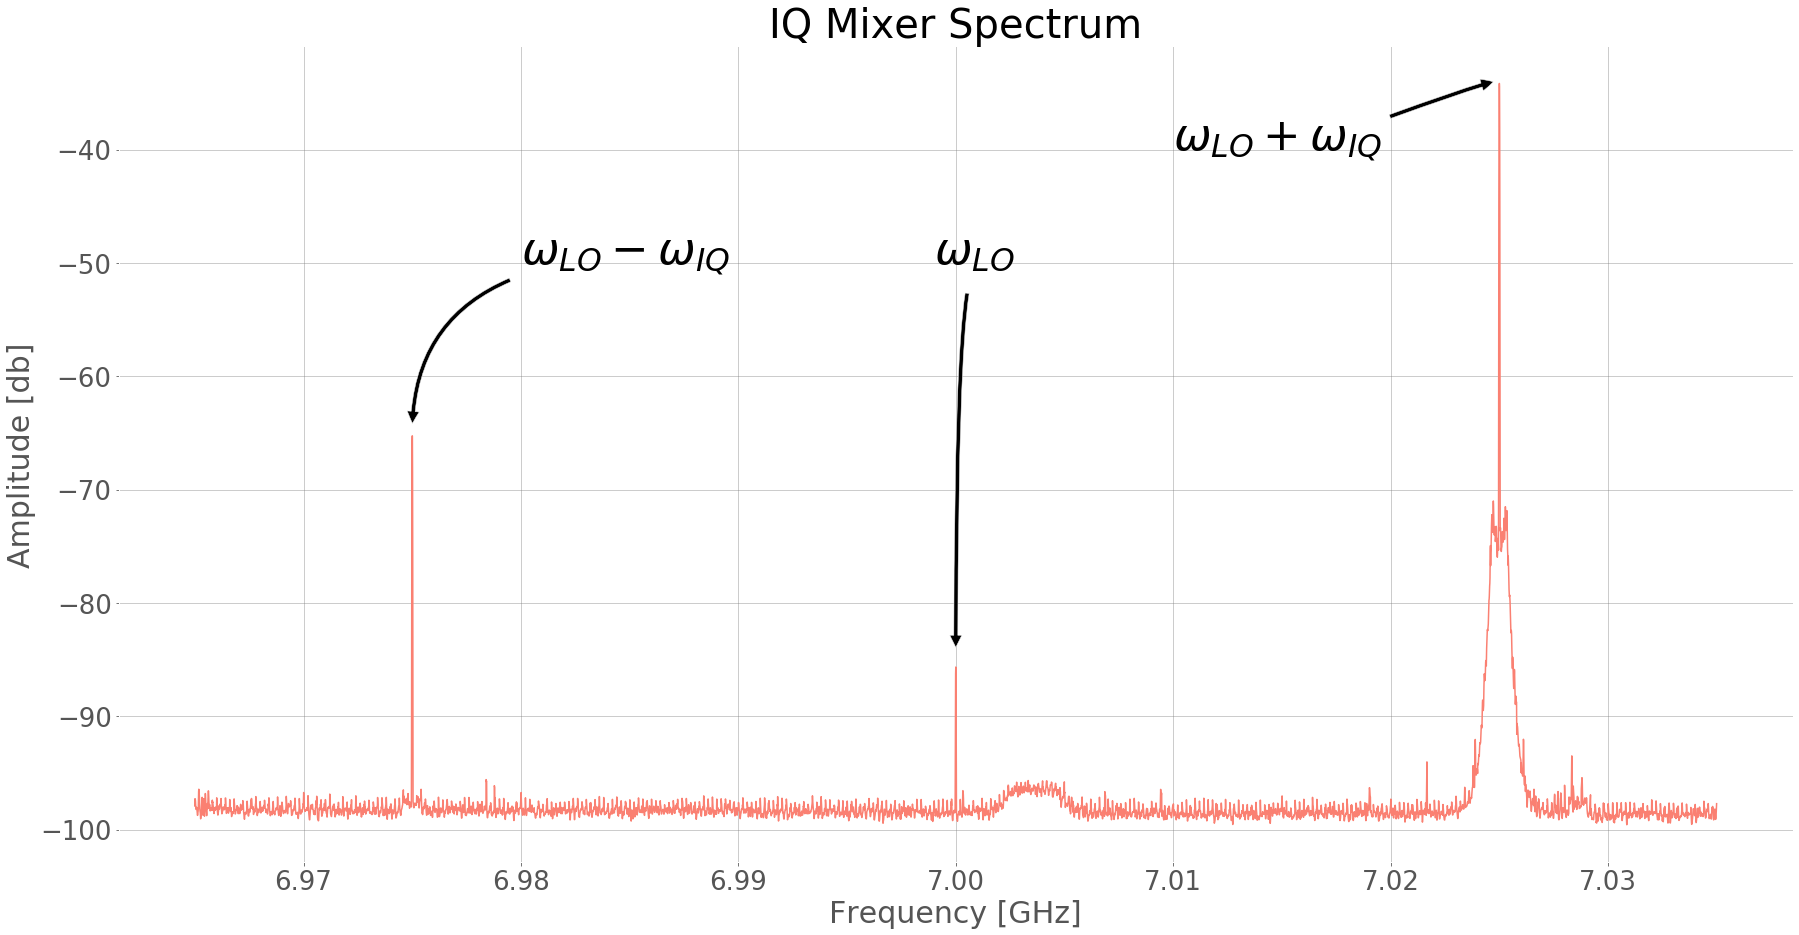
\includegraphics[width=1\columnwidth]{Results/IQ-mixer_after.png} 
%     \caption{Spectrum Around the LO Frequency of the optimized IQ mixer}
%     \label{fig:closeup-spectrum-no-corrections}
% \end{figure}
\begin{figure}[H]
    \begin{center}
        %% Creator: Matplotlib, PGF backend
%%
%% To include the figure in your LaTeX document, write
%%   \input{<filename>.pgf}
%%
%% Make sure the required packages are loaded in your preamble
%%   \usepackage{pgf}
%%
%% and, on pdftex
%%   \usepackage[utf8]{inputenc}\DeclareUnicodeCharacter{2212}{-}
%%
%% or, on luatex and xetex
%%   \usepackage{unicode-math}
%%
%% Figures using additional raster images can only be included by \input if
%% they are in the same directory as the main LaTeX file. For loading figures
%% from other directories you can use the `import` package
%%   \usepackage{import}
%%
%% and then include the figures with
%%   \import{<path to file>}{<filename>.pgf}
%%
%% Matplotlib used the following preamble
%%
\begingroup%
\makeatletter%
\begin{pgfpicture}%
\pgfpathrectangle{\pgfpointorigin}{\pgfqpoint{4.650000in}{2.400000in}}%
\pgfusepath{use as bounding box, clip}%
\begin{pgfscope}%
\pgfsetbuttcap%
\pgfsetmiterjoin%
\definecolor{currentfill}{rgb}{1.000000,1.000000,1.000000}%
\pgfsetfillcolor{currentfill}%
\pgfsetlinewidth{0.000000pt}%
\definecolor{currentstroke}{rgb}{1.000000,1.000000,1.000000}%
\pgfsetstrokecolor{currentstroke}%
\pgfsetdash{}{0pt}%
\pgfpathmoveto{\pgfqpoint{0.000000in}{0.000000in}}%
\pgfpathlineto{\pgfqpoint{4.650000in}{0.000000in}}%
\pgfpathlineto{\pgfqpoint{4.650000in}{2.400000in}}%
\pgfpathlineto{\pgfqpoint{0.000000in}{2.400000in}}%
\pgfpathclose%
\pgfusepath{fill}%
\end{pgfscope}%
\begin{pgfscope}%
\pgfsetbuttcap%
\pgfsetmiterjoin%
\definecolor{currentfill}{rgb}{1.000000,1.000000,1.000000}%
\pgfsetfillcolor{currentfill}%
\pgfsetlinewidth{0.000000pt}%
\definecolor{currentstroke}{rgb}{0.000000,0.000000,0.000000}%
\pgfsetstrokecolor{currentstroke}%
\pgfsetstrokeopacity{0.000000}%
\pgfsetdash{}{0pt}%
\pgfpathmoveto{\pgfqpoint{0.815516in}{0.604117in}}%
\pgfpathlineto{\pgfqpoint{4.500000in}{0.604117in}}%
\pgfpathlineto{\pgfqpoint{4.500000in}{2.176922in}}%
\pgfpathlineto{\pgfqpoint{0.815516in}{2.176922in}}%
\pgfpathclose%
\pgfusepath{fill}%
\end{pgfscope}%
\begin{pgfscope}%
\pgfpathrectangle{\pgfqpoint{0.815516in}{0.604117in}}{\pgfqpoint{3.684484in}{1.572806in}}%
\pgfusepath{clip}%
\pgfsetrectcap%
\pgfsetroundjoin%
\pgfsetlinewidth{0.803000pt}%
\definecolor{currentstroke}{rgb}{0.501961,0.501961,0.501961}%
\pgfsetstrokecolor{currentstroke}%
\pgfsetstrokeopacity{0.200000}%
\pgfsetdash{}{0pt}%
\pgfpathmoveto{\pgfqpoint{1.461550in}{0.604117in}}%
\pgfpathlineto{\pgfqpoint{1.461550in}{2.176922in}}%
\pgfusepath{stroke}%
\end{pgfscope}%
\begin{pgfscope}%
\pgfsetbuttcap%
\pgfsetroundjoin%
\definecolor{currentfill}{rgb}{0.333333,0.333333,0.333333}%
\pgfsetfillcolor{currentfill}%
\pgfsetlinewidth{0.803000pt}%
\definecolor{currentstroke}{rgb}{0.333333,0.333333,0.333333}%
\pgfsetstrokecolor{currentstroke}%
\pgfsetdash{}{0pt}%
\pgfsys@defobject{currentmarker}{\pgfqpoint{0.000000in}{-0.048611in}}{\pgfqpoint{0.000000in}{0.000000in}}{%
\pgfpathmoveto{\pgfqpoint{0.000000in}{0.000000in}}%
\pgfpathlineto{\pgfqpoint{0.000000in}{-0.048611in}}%
\pgfusepath{stroke,fill}%
}%
\begin{pgfscope}%
\pgfsys@transformshift{1.461550in}{0.604117in}%
\pgfsys@useobject{currentmarker}{}%
\end{pgfscope}%
\end{pgfscope}%
\begin{pgfscope}%
\definecolor{textcolor}{rgb}{0.333333,0.333333,0.333333}%
\pgfsetstrokecolor{textcolor}%
\pgfsetfillcolor{textcolor}%
\pgftext[x=1.461550in,y=0.506895in,,top]{\color{textcolor}\rmfamily\fontsize{11.000000}{13.200000}\selectfont \(\displaystyle {6.975}\)}%
\end{pgfscope}%
\begin{pgfscope}%
\pgfpathrectangle{\pgfqpoint{0.815516in}{0.604117in}}{\pgfqpoint{3.684484in}{1.572806in}}%
\pgfusepath{clip}%
\pgfsetrectcap%
\pgfsetroundjoin%
\pgfsetlinewidth{0.803000pt}%
\definecolor{currentstroke}{rgb}{0.501961,0.501961,0.501961}%
\pgfsetstrokecolor{currentstroke}%
\pgfsetstrokeopacity{0.200000}%
\pgfsetdash{}{0pt}%
\pgfpathmoveto{\pgfqpoint{2.657942in}{0.604117in}}%
\pgfpathlineto{\pgfqpoint{2.657942in}{2.176922in}}%
\pgfusepath{stroke}%
\end{pgfscope}%
\begin{pgfscope}%
\pgfsetbuttcap%
\pgfsetroundjoin%
\definecolor{currentfill}{rgb}{0.333333,0.333333,0.333333}%
\pgfsetfillcolor{currentfill}%
\pgfsetlinewidth{0.803000pt}%
\definecolor{currentstroke}{rgb}{0.333333,0.333333,0.333333}%
\pgfsetstrokecolor{currentstroke}%
\pgfsetdash{}{0pt}%
\pgfsys@defobject{currentmarker}{\pgfqpoint{0.000000in}{-0.048611in}}{\pgfqpoint{0.000000in}{0.000000in}}{%
\pgfpathmoveto{\pgfqpoint{0.000000in}{0.000000in}}%
\pgfpathlineto{\pgfqpoint{0.000000in}{-0.048611in}}%
\pgfusepath{stroke,fill}%
}%
\begin{pgfscope}%
\pgfsys@transformshift{2.657942in}{0.604117in}%
\pgfsys@useobject{currentmarker}{}%
\end{pgfscope}%
\end{pgfscope}%
\begin{pgfscope}%
\definecolor{textcolor}{rgb}{0.333333,0.333333,0.333333}%
\pgfsetstrokecolor{textcolor}%
\pgfsetfillcolor{textcolor}%
\pgftext[x=2.657942in,y=0.506895in,,top]{\color{textcolor}\rmfamily\fontsize{11.000000}{13.200000}\selectfont \(\displaystyle {7.000}\)}%
\end{pgfscope}%
\begin{pgfscope}%
\pgfpathrectangle{\pgfqpoint{0.815516in}{0.604117in}}{\pgfqpoint{3.684484in}{1.572806in}}%
\pgfusepath{clip}%
\pgfsetrectcap%
\pgfsetroundjoin%
\pgfsetlinewidth{0.803000pt}%
\definecolor{currentstroke}{rgb}{0.501961,0.501961,0.501961}%
\pgfsetstrokecolor{currentstroke}%
\pgfsetstrokeopacity{0.200000}%
\pgfsetdash{}{0pt}%
\pgfpathmoveto{\pgfqpoint{3.854335in}{0.604117in}}%
\pgfpathlineto{\pgfqpoint{3.854335in}{2.176922in}}%
\pgfusepath{stroke}%
\end{pgfscope}%
\begin{pgfscope}%
\pgfsetbuttcap%
\pgfsetroundjoin%
\definecolor{currentfill}{rgb}{0.333333,0.333333,0.333333}%
\pgfsetfillcolor{currentfill}%
\pgfsetlinewidth{0.803000pt}%
\definecolor{currentstroke}{rgb}{0.333333,0.333333,0.333333}%
\pgfsetstrokecolor{currentstroke}%
\pgfsetdash{}{0pt}%
\pgfsys@defobject{currentmarker}{\pgfqpoint{0.000000in}{-0.048611in}}{\pgfqpoint{0.000000in}{0.000000in}}{%
\pgfpathmoveto{\pgfqpoint{0.000000in}{0.000000in}}%
\pgfpathlineto{\pgfqpoint{0.000000in}{-0.048611in}}%
\pgfusepath{stroke,fill}%
}%
\begin{pgfscope}%
\pgfsys@transformshift{3.854335in}{0.604117in}%
\pgfsys@useobject{currentmarker}{}%
\end{pgfscope}%
\end{pgfscope}%
\begin{pgfscope}%
\definecolor{textcolor}{rgb}{0.333333,0.333333,0.333333}%
\pgfsetstrokecolor{textcolor}%
\pgfsetfillcolor{textcolor}%
\pgftext[x=3.854335in,y=0.506895in,,top]{\color{textcolor}\rmfamily\fontsize{11.000000}{13.200000}\selectfont \(\displaystyle {7.025}\)}%
\end{pgfscope}%
\begin{pgfscope}%
\definecolor{textcolor}{rgb}{0.333333,0.333333,0.333333}%
\pgfsetstrokecolor{textcolor}%
\pgfsetfillcolor{textcolor}%
\pgftext[x=2.657758in,y=0.316154in,,top]{\color{textcolor}\rmfamily\fontsize{12.000000}{14.400000}\selectfont Frequency (GHz)}%
\end{pgfscope}%
\begin{pgfscope}%
\pgfpathrectangle{\pgfqpoint{0.815516in}{0.604117in}}{\pgfqpoint{3.684484in}{1.572806in}}%
\pgfusepath{clip}%
\pgfsetrectcap%
\pgfsetroundjoin%
\pgfsetlinewidth{0.803000pt}%
\definecolor{currentstroke}{rgb}{0.501961,0.501961,0.501961}%
\pgfsetstrokecolor{currentstroke}%
\pgfsetstrokeopacity{0.200000}%
\pgfsetdash{}{0pt}%
\pgfpathmoveto{\pgfqpoint{0.815516in}{0.666264in}}%
\pgfpathlineto{\pgfqpoint{4.500000in}{0.666264in}}%
\pgfusepath{stroke}%
\end{pgfscope}%
\begin{pgfscope}%
\pgfsetbuttcap%
\pgfsetroundjoin%
\definecolor{currentfill}{rgb}{0.333333,0.333333,0.333333}%
\pgfsetfillcolor{currentfill}%
\pgfsetlinewidth{0.803000pt}%
\definecolor{currentstroke}{rgb}{0.333333,0.333333,0.333333}%
\pgfsetstrokecolor{currentstroke}%
\pgfsetdash{}{0pt}%
\pgfsys@defobject{currentmarker}{\pgfqpoint{-0.048611in}{0.000000in}}{\pgfqpoint{0.000000in}{0.000000in}}{%
\pgfpathmoveto{\pgfqpoint{0.000000in}{0.000000in}}%
\pgfpathlineto{\pgfqpoint{-0.048611in}{0.000000in}}%
\pgfusepath{stroke,fill}%
}%
\begin{pgfscope}%
\pgfsys@transformshift{0.815516in}{0.666264in}%
\pgfsys@useobject{currentmarker}{}%
\end{pgfscope}%
\end{pgfscope}%
\begin{pgfscope}%
\definecolor{textcolor}{rgb}{0.333333,0.333333,0.333333}%
\pgfsetstrokecolor{textcolor}%
\pgfsetfillcolor{textcolor}%
\pgftext[x=0.371882in, y=0.613457in, left, base]{\color{textcolor}\rmfamily\fontsize{11.000000}{13.200000}\selectfont \(\displaystyle {-100}\)}%
\end{pgfscope}%
\begin{pgfscope}%
\pgfpathrectangle{\pgfqpoint{0.815516in}{0.604117in}}{\pgfqpoint{3.684484in}{1.572806in}}%
\pgfusepath{clip}%
\pgfsetrectcap%
\pgfsetroundjoin%
\pgfsetlinewidth{0.803000pt}%
\definecolor{currentstroke}{rgb}{0.501961,0.501961,0.501961}%
\pgfsetstrokecolor{currentstroke}%
\pgfsetstrokeopacity{0.200000}%
\pgfsetdash{}{0pt}%
\pgfpathmoveto{\pgfqpoint{0.815516in}{1.103405in}}%
\pgfpathlineto{\pgfqpoint{4.500000in}{1.103405in}}%
\pgfusepath{stroke}%
\end{pgfscope}%
\begin{pgfscope}%
\pgfsetbuttcap%
\pgfsetroundjoin%
\definecolor{currentfill}{rgb}{0.333333,0.333333,0.333333}%
\pgfsetfillcolor{currentfill}%
\pgfsetlinewidth{0.803000pt}%
\definecolor{currentstroke}{rgb}{0.333333,0.333333,0.333333}%
\pgfsetstrokecolor{currentstroke}%
\pgfsetdash{}{0pt}%
\pgfsys@defobject{currentmarker}{\pgfqpoint{-0.048611in}{0.000000in}}{\pgfqpoint{0.000000in}{0.000000in}}{%
\pgfpathmoveto{\pgfqpoint{0.000000in}{0.000000in}}%
\pgfpathlineto{\pgfqpoint{-0.048611in}{0.000000in}}%
\pgfusepath{stroke,fill}%
}%
\begin{pgfscope}%
\pgfsys@transformshift{0.815516in}{1.103405in}%
\pgfsys@useobject{currentmarker}{}%
\end{pgfscope}%
\end{pgfscope}%
\begin{pgfscope}%
\definecolor{textcolor}{rgb}{0.333333,0.333333,0.333333}%
\pgfsetstrokecolor{textcolor}%
\pgfsetfillcolor{textcolor}%
\pgftext[x=0.447923in, y=1.050599in, left, base]{\color{textcolor}\rmfamily\fontsize{11.000000}{13.200000}\selectfont \(\displaystyle {-80}\)}%
\end{pgfscope}%
\begin{pgfscope}%
\pgfpathrectangle{\pgfqpoint{0.815516in}{0.604117in}}{\pgfqpoint{3.684484in}{1.572806in}}%
\pgfusepath{clip}%
\pgfsetrectcap%
\pgfsetroundjoin%
\pgfsetlinewidth{0.803000pt}%
\definecolor{currentstroke}{rgb}{0.501961,0.501961,0.501961}%
\pgfsetstrokecolor{currentstroke}%
\pgfsetstrokeopacity{0.200000}%
\pgfsetdash{}{0pt}%
\pgfpathmoveto{\pgfqpoint{0.815516in}{1.540546in}}%
\pgfpathlineto{\pgfqpoint{4.500000in}{1.540546in}}%
\pgfusepath{stroke}%
\end{pgfscope}%
\begin{pgfscope}%
\pgfsetbuttcap%
\pgfsetroundjoin%
\definecolor{currentfill}{rgb}{0.333333,0.333333,0.333333}%
\pgfsetfillcolor{currentfill}%
\pgfsetlinewidth{0.803000pt}%
\definecolor{currentstroke}{rgb}{0.333333,0.333333,0.333333}%
\pgfsetstrokecolor{currentstroke}%
\pgfsetdash{}{0pt}%
\pgfsys@defobject{currentmarker}{\pgfqpoint{-0.048611in}{0.000000in}}{\pgfqpoint{0.000000in}{0.000000in}}{%
\pgfpathmoveto{\pgfqpoint{0.000000in}{0.000000in}}%
\pgfpathlineto{\pgfqpoint{-0.048611in}{0.000000in}}%
\pgfusepath{stroke,fill}%
}%
\begin{pgfscope}%
\pgfsys@transformshift{0.815516in}{1.540546in}%
\pgfsys@useobject{currentmarker}{}%
\end{pgfscope}%
\end{pgfscope}%
\begin{pgfscope}%
\definecolor{textcolor}{rgb}{0.333333,0.333333,0.333333}%
\pgfsetstrokecolor{textcolor}%
\pgfsetfillcolor{textcolor}%
\pgftext[x=0.447923in, y=1.487740in, left, base]{\color{textcolor}\rmfamily\fontsize{11.000000}{13.200000}\selectfont \(\displaystyle {-60}\)}%
\end{pgfscope}%
\begin{pgfscope}%
\pgfpathrectangle{\pgfqpoint{0.815516in}{0.604117in}}{\pgfqpoint{3.684484in}{1.572806in}}%
\pgfusepath{clip}%
\pgfsetrectcap%
\pgfsetroundjoin%
\pgfsetlinewidth{0.803000pt}%
\definecolor{currentstroke}{rgb}{0.501961,0.501961,0.501961}%
\pgfsetstrokecolor{currentstroke}%
\pgfsetstrokeopacity{0.200000}%
\pgfsetdash{}{0pt}%
\pgfpathmoveto{\pgfqpoint{0.815516in}{1.977688in}}%
\pgfpathlineto{\pgfqpoint{4.500000in}{1.977688in}}%
\pgfusepath{stroke}%
\end{pgfscope}%
\begin{pgfscope}%
\pgfsetbuttcap%
\pgfsetroundjoin%
\definecolor{currentfill}{rgb}{0.333333,0.333333,0.333333}%
\pgfsetfillcolor{currentfill}%
\pgfsetlinewidth{0.803000pt}%
\definecolor{currentstroke}{rgb}{0.333333,0.333333,0.333333}%
\pgfsetstrokecolor{currentstroke}%
\pgfsetdash{}{0pt}%
\pgfsys@defobject{currentmarker}{\pgfqpoint{-0.048611in}{0.000000in}}{\pgfqpoint{0.000000in}{0.000000in}}{%
\pgfpathmoveto{\pgfqpoint{0.000000in}{0.000000in}}%
\pgfpathlineto{\pgfqpoint{-0.048611in}{0.000000in}}%
\pgfusepath{stroke,fill}%
}%
\begin{pgfscope}%
\pgfsys@transformshift{0.815516in}{1.977688in}%
\pgfsys@useobject{currentmarker}{}%
\end{pgfscope}%
\end{pgfscope}%
\begin{pgfscope}%
\definecolor{textcolor}{rgb}{0.333333,0.333333,0.333333}%
\pgfsetstrokecolor{textcolor}%
\pgfsetfillcolor{textcolor}%
\pgftext[x=0.447923in, y=1.924881in, left, base]{\color{textcolor}\rmfamily\fontsize{11.000000}{13.200000}\selectfont \(\displaystyle {-40}\)}%
\end{pgfscope}%
\begin{pgfscope}%
\definecolor{textcolor}{rgb}{0.333333,0.333333,0.333333}%
\pgfsetstrokecolor{textcolor}%
\pgfsetfillcolor{textcolor}%
\pgftext[x=0.316326in,y=1.390520in,,bottom,rotate=90.000000]{\color{textcolor}\rmfamily\fontsize{12.000000}{14.400000}\selectfont Amplitude (db)}%
\end{pgfscope}%
\begin{pgfscope}%
\pgfpathrectangle{\pgfqpoint{0.815516in}{0.604117in}}{\pgfqpoint{3.684484in}{1.572806in}}%
\pgfusepath{clip}%
\pgfsetrectcap%
\pgfsetroundjoin%
\pgfsetlinewidth{1.003750pt}%
\definecolor{currentstroke}{rgb}{0.886275,0.290196,0.200000}%
\pgfsetstrokecolor{currentstroke}%
\pgfsetdash{}{0pt}%
\pgfpathmoveto{\pgfqpoint{0.982993in}{0.711812in}}%
\pgfpathlineto{\pgfqpoint{0.983361in}{0.725766in}}%
\pgfpathlineto{\pgfqpoint{0.984465in}{0.721366in}}%
\pgfpathlineto{\pgfqpoint{0.985938in}{0.705196in}}%
\pgfpathlineto{\pgfqpoint{0.986306in}{0.706383in}}%
\pgfpathlineto{\pgfqpoint{0.987042in}{0.709259in}}%
\pgfpathlineto{\pgfqpoint{0.987410in}{0.708201in}}%
\pgfpathlineto{\pgfqpoint{0.988883in}{0.693671in}}%
\pgfpathlineto{\pgfqpoint{0.989987in}{0.699970in}}%
\pgfpathlineto{\pgfqpoint{0.990723in}{0.707882in}}%
\pgfpathlineto{\pgfqpoint{0.991828in}{0.744090in}}%
\pgfpathlineto{\pgfqpoint{0.992196in}{0.741723in}}%
\pgfpathlineto{\pgfqpoint{0.994405in}{0.702064in}}%
\pgfpathlineto{\pgfqpoint{0.995877in}{0.687022in}}%
\pgfpathlineto{\pgfqpoint{0.996982in}{0.696241in}}%
\pgfpathlineto{\pgfqpoint{0.999190in}{0.728447in}}%
\pgfpathlineto{\pgfqpoint{0.999558in}{0.726146in}}%
\pgfpathlineto{\pgfqpoint{1.000663in}{0.694110in}}%
\pgfpathlineto{\pgfqpoint{1.001399in}{0.697074in}}%
\pgfpathlineto{\pgfqpoint{1.002503in}{0.725960in}}%
\pgfpathlineto{\pgfqpoint{1.003240in}{0.711482in}}%
\pgfpathlineto{\pgfqpoint{1.004344in}{0.692007in}}%
\pgfpathlineto{\pgfqpoint{1.004712in}{0.694027in}}%
\pgfpathlineto{\pgfqpoint{1.006184in}{0.735796in}}%
\pgfpathlineto{\pgfqpoint{1.006921in}{0.722273in}}%
\pgfpathlineto{\pgfqpoint{1.009129in}{0.693085in}}%
\pgfpathlineto{\pgfqpoint{1.012811in}{0.740996in}}%
\pgfpathlineto{\pgfqpoint{1.013915in}{0.724428in}}%
\pgfpathlineto{\pgfqpoint{1.014651in}{0.707445in}}%
\pgfpathlineto{\pgfqpoint{1.015756in}{0.714583in}}%
\pgfpathlineto{\pgfqpoint{1.016860in}{0.702295in}}%
\pgfpathlineto{\pgfqpoint{1.017964in}{0.706903in}}%
\pgfpathlineto{\pgfqpoint{1.019805in}{0.708437in}}%
\pgfpathlineto{\pgfqpoint{1.020173in}{0.707716in}}%
\pgfpathlineto{\pgfqpoint{1.020909in}{0.703202in}}%
\pgfpathlineto{\pgfqpoint{1.021646in}{0.722994in}}%
\pgfpathlineto{\pgfqpoint{1.022382in}{0.719862in}}%
\pgfpathlineto{\pgfqpoint{1.025327in}{0.697284in}}%
\pgfpathlineto{\pgfqpoint{1.025695in}{0.700092in}}%
\pgfpathlineto{\pgfqpoint{1.026431in}{0.708643in}}%
\pgfpathlineto{\pgfqpoint{1.027167in}{0.704422in}}%
\pgfpathlineto{\pgfqpoint{1.027535in}{0.703154in}}%
\pgfpathlineto{\pgfqpoint{1.027904in}{0.705220in}}%
\pgfpathlineto{\pgfqpoint{1.029008in}{0.709628in}}%
\pgfpathlineto{\pgfqpoint{1.029376in}{0.706627in}}%
\pgfpathlineto{\pgfqpoint{1.029744in}{0.705069in}}%
\pgfpathlineto{\pgfqpoint{1.030112in}{0.706960in}}%
\pgfpathlineto{\pgfqpoint{1.030849in}{0.709985in}}%
\pgfpathlineto{\pgfqpoint{1.031217in}{0.727484in}}%
\pgfpathlineto{\pgfqpoint{1.032321in}{0.706813in}}%
\pgfpathlineto{\pgfqpoint{1.033794in}{0.694280in}}%
\pgfpathlineto{\pgfqpoint{1.034530in}{0.697399in}}%
\pgfpathlineto{\pgfqpoint{1.036370in}{0.712212in}}%
\pgfpathlineto{\pgfqpoint{1.037107in}{0.706381in}}%
\pgfpathlineto{\pgfqpoint{1.037475in}{0.706029in}}%
\pgfpathlineto{\pgfqpoint{1.038947in}{0.715687in}}%
\pgfpathlineto{\pgfqpoint{1.040052in}{0.712955in}}%
\pgfpathlineto{\pgfqpoint{1.040420in}{0.712199in}}%
\pgfpathlineto{\pgfqpoint{1.040788in}{0.726155in}}%
\pgfpathlineto{\pgfqpoint{1.041524in}{0.709672in}}%
\pgfpathlineto{\pgfqpoint{1.042628in}{0.696718in}}%
\pgfpathlineto{\pgfqpoint{1.043365in}{0.700483in}}%
\pgfpathlineto{\pgfqpoint{1.043733in}{0.699854in}}%
\pgfpathlineto{\pgfqpoint{1.044101in}{0.701620in}}%
\pgfpathlineto{\pgfqpoint{1.045573in}{0.710055in}}%
\pgfpathlineto{\pgfqpoint{1.045942in}{0.708549in}}%
\pgfpathlineto{\pgfqpoint{1.046678in}{0.704693in}}%
\pgfpathlineto{\pgfqpoint{1.047414in}{0.708547in}}%
\pgfpathlineto{\pgfqpoint{1.048150in}{0.704711in}}%
\pgfpathlineto{\pgfqpoint{1.048887in}{0.707318in}}%
\pgfpathlineto{\pgfqpoint{1.050727in}{0.727175in}}%
\pgfpathlineto{\pgfqpoint{1.051095in}{0.721912in}}%
\pgfpathlineto{\pgfqpoint{1.052568in}{0.697456in}}%
\pgfpathlineto{\pgfqpoint{1.053672in}{0.702975in}}%
\pgfpathlineto{\pgfqpoint{1.054776in}{0.708385in}}%
\pgfpathlineto{\pgfqpoint{1.055513in}{0.704411in}}%
\pgfpathlineto{\pgfqpoint{1.056985in}{0.697900in}}%
\pgfpathlineto{\pgfqpoint{1.057353in}{0.698586in}}%
\pgfpathlineto{\pgfqpoint{1.059930in}{0.724253in}}%
\pgfpathlineto{\pgfqpoint{1.060298in}{0.717549in}}%
\pgfpathlineto{\pgfqpoint{1.061771in}{0.701168in}}%
\pgfpathlineto{\pgfqpoint{1.062139in}{0.703395in}}%
\pgfpathlineto{\pgfqpoint{1.062875in}{0.708632in}}%
\pgfpathlineto{\pgfqpoint{1.063243in}{0.703898in}}%
\pgfpathlineto{\pgfqpoint{1.063979in}{0.691378in}}%
\pgfpathlineto{\pgfqpoint{1.064716in}{0.697410in}}%
\pgfpathlineto{\pgfqpoint{1.065084in}{0.700595in}}%
\pgfpathlineto{\pgfqpoint{1.066188in}{0.700103in}}%
\pgfpathlineto{\pgfqpoint{1.066924in}{0.697137in}}%
\pgfpathlineto{\pgfqpoint{1.067661in}{0.699489in}}%
\pgfpathlineto{\pgfqpoint{1.068765in}{0.703227in}}%
\pgfpathlineto{\pgfqpoint{1.069501in}{0.725433in}}%
\pgfpathlineto{\pgfqpoint{1.070238in}{0.715440in}}%
\pgfpathlineto{\pgfqpoint{1.072078in}{0.696342in}}%
\pgfpathlineto{\pgfqpoint{1.072814in}{0.697699in}}%
\pgfpathlineto{\pgfqpoint{1.075023in}{0.705666in}}%
\pgfpathlineto{\pgfqpoint{1.076127in}{0.712435in}}%
\pgfpathlineto{\pgfqpoint{1.076496in}{0.706809in}}%
\pgfpathlineto{\pgfqpoint{1.076864in}{0.702553in}}%
\pgfpathlineto{\pgfqpoint{1.077600in}{0.708627in}}%
\pgfpathlineto{\pgfqpoint{1.078336in}{0.707948in}}%
\pgfpathlineto{\pgfqpoint{1.078704in}{0.696975in}}%
\pgfpathlineto{\pgfqpoint{1.079072in}{0.709633in}}%
\pgfpathlineto{\pgfqpoint{1.079809in}{0.705994in}}%
\pgfpathlineto{\pgfqpoint{1.080913in}{0.703576in}}%
\pgfpathlineto{\pgfqpoint{1.082017in}{0.697093in}}%
\pgfpathlineto{\pgfqpoint{1.082754in}{0.700206in}}%
\pgfpathlineto{\pgfqpoint{1.083858in}{0.715053in}}%
\pgfpathlineto{\pgfqpoint{1.084594in}{0.707657in}}%
\pgfpathlineto{\pgfqpoint{1.084962in}{0.703465in}}%
\pgfpathlineto{\pgfqpoint{1.085699in}{0.706770in}}%
\pgfpathlineto{\pgfqpoint{1.086435in}{0.709312in}}%
\pgfpathlineto{\pgfqpoint{1.086803in}{0.707355in}}%
\pgfpathlineto{\pgfqpoint{1.087171in}{0.705646in}}%
\pgfpathlineto{\pgfqpoint{1.087539in}{0.708227in}}%
\pgfpathlineto{\pgfqpoint{1.088644in}{0.722056in}}%
\pgfpathlineto{\pgfqpoint{1.089380in}{0.719005in}}%
\pgfpathlineto{\pgfqpoint{1.092325in}{0.686202in}}%
\pgfpathlineto{\pgfqpoint{1.094902in}{0.699301in}}%
\pgfpathlineto{\pgfqpoint{1.095638in}{0.696197in}}%
\pgfpathlineto{\pgfqpoint{1.096006in}{0.698409in}}%
\pgfpathlineto{\pgfqpoint{1.098215in}{0.720935in}}%
\pgfpathlineto{\pgfqpoint{1.098951in}{0.710575in}}%
\pgfpathlineto{\pgfqpoint{1.101160in}{0.692348in}}%
\pgfpathlineto{\pgfqpoint{1.101528in}{0.692919in}}%
\pgfpathlineto{\pgfqpoint{1.103000in}{0.705447in}}%
\pgfpathlineto{\pgfqpoint{1.104105in}{0.700779in}}%
\pgfpathlineto{\pgfqpoint{1.107050in}{0.723468in}}%
\pgfpathlineto{\pgfqpoint{1.107418in}{0.707718in}}%
\pgfpathlineto{\pgfqpoint{1.107786in}{0.726264in}}%
\pgfpathlineto{\pgfqpoint{1.108522in}{0.715025in}}%
\pgfpathlineto{\pgfqpoint{1.110363in}{0.706057in}}%
\pgfpathlineto{\pgfqpoint{1.110731in}{0.707924in}}%
\pgfpathlineto{\pgfqpoint{1.111099in}{0.710332in}}%
\pgfpathlineto{\pgfqpoint{1.111467in}{0.704636in}}%
\pgfpathlineto{\pgfqpoint{1.112203in}{0.695465in}}%
\pgfpathlineto{\pgfqpoint{1.112940in}{0.700311in}}%
\pgfpathlineto{\pgfqpoint{1.113676in}{0.705432in}}%
\pgfpathlineto{\pgfqpoint{1.114412in}{0.701447in}}%
\pgfpathlineto{\pgfqpoint{1.115148in}{0.700090in}}%
\pgfpathlineto{\pgfqpoint{1.115516in}{0.701751in}}%
\pgfpathlineto{\pgfqpoint{1.117357in}{0.729894in}}%
\pgfpathlineto{\pgfqpoint{1.118093in}{0.717143in}}%
\pgfpathlineto{\pgfqpoint{1.120302in}{0.693338in}}%
\pgfpathlineto{\pgfqpoint{1.121038in}{0.695904in}}%
\pgfpathlineto{\pgfqpoint{1.122143in}{0.705758in}}%
\pgfpathlineto{\pgfqpoint{1.122879in}{0.700641in}}%
\pgfpathlineto{\pgfqpoint{1.123615in}{0.699063in}}%
\pgfpathlineto{\pgfqpoint{1.123983in}{0.699631in}}%
\pgfpathlineto{\pgfqpoint{1.126928in}{0.720494in}}%
\pgfpathlineto{\pgfqpoint{1.127296in}{0.714245in}}%
\pgfpathlineto{\pgfqpoint{1.128401in}{0.698324in}}%
\pgfpathlineto{\pgfqpoint{1.129137in}{0.702949in}}%
\pgfpathlineto{\pgfqpoint{1.129505in}{0.703959in}}%
\pgfpathlineto{\pgfqpoint{1.129873in}{0.702077in}}%
\pgfpathlineto{\pgfqpoint{1.130241in}{0.701342in}}%
\pgfpathlineto{\pgfqpoint{1.130609in}{0.702267in}}%
\pgfpathlineto{\pgfqpoint{1.131346in}{0.709631in}}%
\pgfpathlineto{\pgfqpoint{1.132082in}{0.706831in}}%
\pgfpathlineto{\pgfqpoint{1.132818in}{0.702024in}}%
\pgfpathlineto{\pgfqpoint{1.133554in}{0.707738in}}%
\pgfpathlineto{\pgfqpoint{1.133922in}{0.708756in}}%
\pgfpathlineto{\pgfqpoint{1.134659in}{0.707615in}}%
\pgfpathlineto{\pgfqpoint{1.135027in}{0.707130in}}%
\pgfpathlineto{\pgfqpoint{1.136499in}{0.722784in}}%
\pgfpathlineto{\pgfqpoint{1.137235in}{0.711526in}}%
\pgfpathlineto{\pgfqpoint{1.139444in}{0.699367in}}%
\pgfpathlineto{\pgfqpoint{1.139812in}{0.701581in}}%
\pgfpathlineto{\pgfqpoint{1.140549in}{0.705570in}}%
\pgfpathlineto{\pgfqpoint{1.141285in}{0.701673in}}%
\pgfpathlineto{\pgfqpoint{1.143125in}{0.696289in}}%
\pgfpathlineto{\pgfqpoint{1.143494in}{0.698265in}}%
\pgfpathlineto{\pgfqpoint{1.146070in}{0.727538in}}%
\pgfpathlineto{\pgfqpoint{1.146439in}{0.725783in}}%
\pgfpathlineto{\pgfqpoint{1.149383in}{0.693046in}}%
\pgfpathlineto{\pgfqpoint{1.149752in}{0.695190in}}%
\pgfpathlineto{\pgfqpoint{1.150488in}{0.700938in}}%
\pgfpathlineto{\pgfqpoint{1.151592in}{0.700086in}}%
\pgfpathlineto{\pgfqpoint{1.151960in}{0.701041in}}%
\pgfpathlineto{\pgfqpoint{1.152328in}{0.699651in}}%
\pgfpathlineto{\pgfqpoint{1.153065in}{0.694916in}}%
\pgfpathlineto{\pgfqpoint{1.153433in}{0.695795in}}%
\pgfpathlineto{\pgfqpoint{1.155642in}{0.720502in}}%
\pgfpathlineto{\pgfqpoint{1.156010in}{0.711071in}}%
\pgfpathlineto{\pgfqpoint{1.157114in}{0.697216in}}%
\pgfpathlineto{\pgfqpoint{1.157850in}{0.699257in}}%
\pgfpathlineto{\pgfqpoint{1.158955in}{0.694726in}}%
\pgfpathlineto{\pgfqpoint{1.159323in}{0.698001in}}%
\pgfpathlineto{\pgfqpoint{1.162268in}{0.707974in}}%
\pgfpathlineto{\pgfqpoint{1.163004in}{0.704667in}}%
\pgfpathlineto{\pgfqpoint{1.163740in}{0.705775in}}%
\pgfpathlineto{\pgfqpoint{1.165213in}{0.729230in}}%
\pgfpathlineto{\pgfqpoint{1.165581in}{0.718944in}}%
\pgfpathlineto{\pgfqpoint{1.167789in}{0.693470in}}%
\pgfpathlineto{\pgfqpoint{1.168158in}{0.693609in}}%
\pgfpathlineto{\pgfqpoint{1.169262in}{0.701493in}}%
\pgfpathlineto{\pgfqpoint{1.170366in}{0.712472in}}%
\pgfpathlineto{\pgfqpoint{1.171103in}{0.706719in}}%
\pgfpathlineto{\pgfqpoint{1.172207in}{0.691843in}}%
\pgfpathlineto{\pgfqpoint{1.172943in}{0.697085in}}%
\pgfpathlineto{\pgfqpoint{1.174784in}{0.719132in}}%
\pgfpathlineto{\pgfqpoint{1.175888in}{0.711646in}}%
\pgfpathlineto{\pgfqpoint{1.178097in}{0.697148in}}%
\pgfpathlineto{\pgfqpoint{1.178465in}{0.697399in}}%
\pgfpathlineto{\pgfqpoint{1.179938in}{0.703124in}}%
\pgfpathlineto{\pgfqpoint{1.180306in}{0.703025in}}%
\pgfpathlineto{\pgfqpoint{1.182146in}{0.698667in}}%
\pgfpathlineto{\pgfqpoint{1.182514in}{0.698908in}}%
\pgfpathlineto{\pgfqpoint{1.183619in}{0.706394in}}%
\pgfpathlineto{\pgfqpoint{1.184355in}{0.730347in}}%
\pgfpathlineto{\pgfqpoint{1.185459in}{0.713818in}}%
\pgfpathlineto{\pgfqpoint{1.187300in}{0.696811in}}%
\pgfpathlineto{\pgfqpoint{1.187668in}{0.698527in}}%
\pgfpathlineto{\pgfqpoint{1.189509in}{0.716564in}}%
\pgfpathlineto{\pgfqpoint{1.190245in}{0.712138in}}%
\pgfpathlineto{\pgfqpoint{1.192085in}{0.710686in}}%
\pgfpathlineto{\pgfqpoint{1.193190in}{0.712557in}}%
\pgfpathlineto{\pgfqpoint{1.193558in}{0.712068in}}%
\pgfpathlineto{\pgfqpoint{1.193926in}{0.721814in}}%
\pgfpathlineto{\pgfqpoint{1.194662in}{0.712850in}}%
\pgfpathlineto{\pgfqpoint{1.196135in}{0.693623in}}%
\pgfpathlineto{\pgfqpoint{1.196871in}{0.697966in}}%
\pgfpathlineto{\pgfqpoint{1.197607in}{0.695188in}}%
\pgfpathlineto{\pgfqpoint{1.197975in}{0.696232in}}%
\pgfpathlineto{\pgfqpoint{1.200184in}{0.704947in}}%
\pgfpathlineto{\pgfqpoint{1.200552in}{0.703078in}}%
\pgfpathlineto{\pgfqpoint{1.200920in}{0.703710in}}%
\pgfpathlineto{\pgfqpoint{1.203497in}{0.726847in}}%
\pgfpathlineto{\pgfqpoint{1.203865in}{0.718841in}}%
\pgfpathlineto{\pgfqpoint{1.205338in}{0.696398in}}%
\pgfpathlineto{\pgfqpoint{1.206074in}{0.698337in}}%
\pgfpathlineto{\pgfqpoint{1.206810in}{0.696165in}}%
\pgfpathlineto{\pgfqpoint{1.207547in}{0.696523in}}%
\pgfpathlineto{\pgfqpoint{1.208651in}{0.699725in}}%
\pgfpathlineto{\pgfqpoint{1.209019in}{0.698536in}}%
\pgfpathlineto{\pgfqpoint{1.209755in}{0.695509in}}%
\pgfpathlineto{\pgfqpoint{1.210492in}{0.687535in}}%
\pgfpathlineto{\pgfqpoint{1.211228in}{0.691133in}}%
\pgfpathlineto{\pgfqpoint{1.213068in}{0.726111in}}%
\pgfpathlineto{\pgfqpoint{1.213805in}{0.715029in}}%
\pgfpathlineto{\pgfqpoint{1.215645in}{0.696451in}}%
\pgfpathlineto{\pgfqpoint{1.216381in}{0.696593in}}%
\pgfpathlineto{\pgfqpoint{1.216750in}{0.696733in}}%
\pgfpathlineto{\pgfqpoint{1.217486in}{0.703946in}}%
\pgfpathlineto{\pgfqpoint{1.218222in}{0.701196in}}%
\pgfpathlineto{\pgfqpoint{1.218590in}{0.699576in}}%
\pgfpathlineto{\pgfqpoint{1.219326in}{0.702866in}}%
\pgfpathlineto{\pgfqpoint{1.220431in}{0.706802in}}%
\pgfpathlineto{\pgfqpoint{1.222639in}{0.737767in}}%
\pgfpathlineto{\pgfqpoint{1.223008in}{0.729503in}}%
\pgfpathlineto{\pgfqpoint{1.225216in}{0.702420in}}%
\pgfpathlineto{\pgfqpoint{1.225584in}{0.702735in}}%
\pgfpathlineto{\pgfqpoint{1.227057in}{0.703987in}}%
\pgfpathlineto{\pgfqpoint{1.227793in}{0.704682in}}%
\pgfpathlineto{\pgfqpoint{1.228529in}{0.703780in}}%
\pgfpathlineto{\pgfqpoint{1.229266in}{0.703749in}}%
\pgfpathlineto{\pgfqpoint{1.230002in}{0.708787in}}%
\pgfpathlineto{\pgfqpoint{1.230738in}{0.704859in}}%
\pgfpathlineto{\pgfqpoint{1.231106in}{0.703076in}}%
\pgfpathlineto{\pgfqpoint{1.231474in}{0.707174in}}%
\pgfpathlineto{\pgfqpoint{1.232211in}{0.731628in}}%
\pgfpathlineto{\pgfqpoint{1.232947in}{0.718358in}}%
\pgfpathlineto{\pgfqpoint{1.235524in}{0.685092in}}%
\pgfpathlineto{\pgfqpoint{1.235892in}{0.685175in}}%
\pgfpathlineto{\pgfqpoint{1.238837in}{0.713351in}}%
\pgfpathlineto{\pgfqpoint{1.239941in}{0.709559in}}%
\pgfpathlineto{\pgfqpoint{1.241414in}{0.705554in}}%
\pgfpathlineto{\pgfqpoint{1.241782in}{0.714942in}}%
\pgfpathlineto{\pgfqpoint{1.242886in}{0.706024in}}%
\pgfpathlineto{\pgfqpoint{1.243622in}{0.704374in}}%
\pgfpathlineto{\pgfqpoint{1.245463in}{0.695948in}}%
\pgfpathlineto{\pgfqpoint{1.246199in}{0.701965in}}%
\pgfpathlineto{\pgfqpoint{1.246935in}{0.696565in}}%
\pgfpathlineto{\pgfqpoint{1.247304in}{0.694980in}}%
\pgfpathlineto{\pgfqpoint{1.247672in}{0.697430in}}%
\pgfpathlineto{\pgfqpoint{1.250249in}{0.722111in}}%
\pgfpathlineto{\pgfqpoint{1.250617in}{0.720406in}}%
\pgfpathlineto{\pgfqpoint{1.251353in}{0.730539in}}%
\pgfpathlineto{\pgfqpoint{1.253930in}{0.685638in}}%
\pgfpathlineto{\pgfqpoint{1.254298in}{0.686482in}}%
\pgfpathlineto{\pgfqpoint{1.254666in}{0.685476in}}%
\pgfpathlineto{\pgfqpoint{1.255034in}{0.683179in}}%
\pgfpathlineto{\pgfqpoint{1.255402in}{0.683791in}}%
\pgfpathlineto{\pgfqpoint{1.258715in}{0.707694in}}%
\pgfpathlineto{\pgfqpoint{1.259452in}{0.715126in}}%
\pgfpathlineto{\pgfqpoint{1.260188in}{0.712302in}}%
\pgfpathlineto{\pgfqpoint{1.260556in}{0.707410in}}%
\pgfpathlineto{\pgfqpoint{1.260924in}{0.723774in}}%
\pgfpathlineto{\pgfqpoint{1.261660in}{0.705006in}}%
\pgfpathlineto{\pgfqpoint{1.262397in}{0.692069in}}%
\pgfpathlineto{\pgfqpoint{1.263501in}{0.696278in}}%
\pgfpathlineto{\pgfqpoint{1.268286in}{0.716636in}}%
\pgfpathlineto{\pgfqpoint{1.269023in}{0.712205in}}%
\pgfpathlineto{\pgfqpoint{1.269759in}{0.702818in}}%
\pgfpathlineto{\pgfqpoint{1.270127in}{0.707613in}}%
\pgfpathlineto{\pgfqpoint{1.270495in}{0.724050in}}%
\pgfpathlineto{\pgfqpoint{1.271600in}{0.707185in}}%
\pgfpathlineto{\pgfqpoint{1.273808in}{0.691902in}}%
\pgfpathlineto{\pgfqpoint{1.274176in}{0.690329in}}%
\pgfpathlineto{\pgfqpoint{1.274545in}{0.693848in}}%
\pgfpathlineto{\pgfqpoint{1.276017in}{0.709084in}}%
\pgfpathlineto{\pgfqpoint{1.276753in}{0.707972in}}%
\pgfpathlineto{\pgfqpoint{1.277121in}{0.707150in}}%
\pgfpathlineto{\pgfqpoint{1.277489in}{0.707751in}}%
\pgfpathlineto{\pgfqpoint{1.278226in}{0.710761in}}%
\pgfpathlineto{\pgfqpoint{1.278962in}{0.708557in}}%
\pgfpathlineto{\pgfqpoint{1.279330in}{0.708284in}}%
\pgfpathlineto{\pgfqpoint{1.279698in}{0.710708in}}%
\pgfpathlineto{\pgfqpoint{1.280066in}{0.734731in}}%
\pgfpathlineto{\pgfqpoint{1.281171in}{0.710890in}}%
\pgfpathlineto{\pgfqpoint{1.283011in}{0.694197in}}%
\pgfpathlineto{\pgfqpoint{1.283748in}{0.691391in}}%
\pgfpathlineto{\pgfqpoint{1.284116in}{0.693723in}}%
\pgfpathlineto{\pgfqpoint{1.287061in}{0.710739in}}%
\pgfpathlineto{\pgfqpoint{1.287429in}{0.710227in}}%
\pgfpathlineto{\pgfqpoint{1.288533in}{0.714374in}}%
\pgfpathlineto{\pgfqpoint{1.288901in}{0.712793in}}%
\pgfpathlineto{\pgfqpoint{1.289269in}{0.703187in}}%
\pgfpathlineto{\pgfqpoint{1.289637in}{0.715552in}}%
\pgfpathlineto{\pgfqpoint{1.290374in}{0.709191in}}%
\pgfpathlineto{\pgfqpoint{1.291846in}{0.690670in}}%
\pgfpathlineto{\pgfqpoint{1.292951in}{0.694576in}}%
\pgfpathlineto{\pgfqpoint{1.293687in}{0.698429in}}%
\pgfpathlineto{\pgfqpoint{1.294423in}{0.705325in}}%
\pgfpathlineto{\pgfqpoint{1.295159in}{0.699795in}}%
\pgfpathlineto{\pgfqpoint{1.295527in}{0.697058in}}%
\pgfpathlineto{\pgfqpoint{1.296264in}{0.699727in}}%
\pgfpathlineto{\pgfqpoint{1.296632in}{0.701251in}}%
\pgfpathlineto{\pgfqpoint{1.297368in}{0.697880in}}%
\pgfpathlineto{\pgfqpoint{1.298104in}{0.704064in}}%
\pgfpathlineto{\pgfqpoint{1.299209in}{0.718776in}}%
\pgfpathlineto{\pgfqpoint{1.299577in}{0.707500in}}%
\pgfpathlineto{\pgfqpoint{1.300681in}{0.694213in}}%
\pgfpathlineto{\pgfqpoint{1.301417in}{0.700781in}}%
\pgfpathlineto{\pgfqpoint{1.302154in}{0.706254in}}%
\pgfpathlineto{\pgfqpoint{1.302890in}{0.701034in}}%
\pgfpathlineto{\pgfqpoint{1.303994in}{0.705421in}}%
\pgfpathlineto{\pgfqpoint{1.304362in}{0.702252in}}%
\pgfpathlineto{\pgfqpoint{1.305835in}{0.694206in}}%
\pgfpathlineto{\pgfqpoint{1.306203in}{0.694407in}}%
\pgfpathlineto{\pgfqpoint{1.308412in}{0.711130in}}%
\pgfpathlineto{\pgfqpoint{1.308780in}{0.729750in}}%
\pgfpathlineto{\pgfqpoint{1.309884in}{0.714664in}}%
\pgfpathlineto{\pgfqpoint{1.310988in}{0.692296in}}%
\pgfpathlineto{\pgfqpoint{1.311725in}{0.700831in}}%
\pgfpathlineto{\pgfqpoint{1.313933in}{0.707762in}}%
\pgfpathlineto{\pgfqpoint{1.314670in}{0.706634in}}%
\pgfpathlineto{\pgfqpoint{1.316142in}{0.702097in}}%
\pgfpathlineto{\pgfqpoint{1.316510in}{0.703804in}}%
\pgfpathlineto{\pgfqpoint{1.318351in}{0.719447in}}%
\pgfpathlineto{\pgfqpoint{1.319823in}{0.686453in}}%
\pgfpathlineto{\pgfqpoint{1.320560in}{0.691684in}}%
\pgfpathlineto{\pgfqpoint{1.322768in}{0.707458in}}%
\pgfpathlineto{\pgfqpoint{1.323505in}{0.705602in}}%
\pgfpathlineto{\pgfqpoint{1.324241in}{0.700960in}}%
\pgfpathlineto{\pgfqpoint{1.324977in}{0.695598in}}%
\pgfpathlineto{\pgfqpoint{1.325345in}{0.696901in}}%
\pgfpathlineto{\pgfqpoint{1.327922in}{0.723919in}}%
\pgfpathlineto{\pgfqpoint{1.330131in}{0.700040in}}%
\pgfpathlineto{\pgfqpoint{1.330867in}{0.696787in}}%
\pgfpathlineto{\pgfqpoint{1.331603in}{0.700239in}}%
\pgfpathlineto{\pgfqpoint{1.331971in}{0.700477in}}%
\pgfpathlineto{\pgfqpoint{1.332708in}{0.697069in}}%
\pgfpathlineto{\pgfqpoint{1.333812in}{0.698477in}}%
\pgfpathlineto{\pgfqpoint{1.334548in}{0.704464in}}%
\pgfpathlineto{\pgfqpoint{1.335284in}{0.701950in}}%
\pgfpathlineto{\pgfqpoint{1.335653in}{0.699183in}}%
\pgfpathlineto{\pgfqpoint{1.336389in}{0.703978in}}%
\pgfpathlineto{\pgfqpoint{1.336757in}{0.705174in}}%
\pgfpathlineto{\pgfqpoint{1.337493in}{0.731372in}}%
\pgfpathlineto{\pgfqpoint{1.338229in}{0.711130in}}%
\pgfpathlineto{\pgfqpoint{1.340070in}{0.693830in}}%
\pgfpathlineto{\pgfqpoint{1.340438in}{0.694506in}}%
\pgfpathlineto{\pgfqpoint{1.342279in}{0.709836in}}%
\pgfpathlineto{\pgfqpoint{1.343015in}{0.703707in}}%
\pgfpathlineto{\pgfqpoint{1.343751in}{0.699004in}}%
\pgfpathlineto{\pgfqpoint{1.344487in}{0.700717in}}%
\pgfpathlineto{\pgfqpoint{1.347064in}{0.717276in}}%
\pgfpathlineto{\pgfqpoint{1.347432in}{0.712638in}}%
\pgfpathlineto{\pgfqpoint{1.350009in}{0.690895in}}%
\pgfpathlineto{\pgfqpoint{1.350377in}{0.691109in}}%
\pgfpathlineto{\pgfqpoint{1.352218in}{0.708262in}}%
\pgfpathlineto{\pgfqpoint{1.352586in}{0.705373in}}%
\pgfpathlineto{\pgfqpoint{1.353322in}{0.695349in}}%
\pgfpathlineto{\pgfqpoint{1.354059in}{0.702837in}}%
\pgfpathlineto{\pgfqpoint{1.354795in}{0.698702in}}%
\pgfpathlineto{\pgfqpoint{1.355163in}{0.699959in}}%
\pgfpathlineto{\pgfqpoint{1.356635in}{0.721248in}}%
\pgfpathlineto{\pgfqpoint{1.357004in}{0.713528in}}%
\pgfpathlineto{\pgfqpoint{1.359212in}{0.696145in}}%
\pgfpathlineto{\pgfqpoint{1.359949in}{0.698803in}}%
\pgfpathlineto{\pgfqpoint{1.361421in}{0.702715in}}%
\pgfpathlineto{\pgfqpoint{1.362157in}{0.705753in}}%
\pgfpathlineto{\pgfqpoint{1.362894in}{0.703648in}}%
\pgfpathlineto{\pgfqpoint{1.365470in}{0.710426in}}%
\pgfpathlineto{\pgfqpoint{1.365838in}{0.708321in}}%
\pgfpathlineto{\pgfqpoint{1.366207in}{0.722843in}}%
\pgfpathlineto{\pgfqpoint{1.367311in}{0.706925in}}%
\pgfpathlineto{\pgfqpoint{1.368047in}{0.697716in}}%
\pgfpathlineto{\pgfqpoint{1.369152in}{0.700486in}}%
\pgfpathlineto{\pgfqpoint{1.372097in}{0.695386in}}%
\pgfpathlineto{\pgfqpoint{1.372465in}{0.695743in}}%
\pgfpathlineto{\pgfqpoint{1.375041in}{0.708074in}}%
\pgfpathlineto{\pgfqpoint{1.373569in}{0.695349in}}%
\pgfpathlineto{\pgfqpoint{1.375410in}{0.702523in}}%
\pgfpathlineto{\pgfqpoint{1.375778in}{0.719563in}}%
\pgfpathlineto{\pgfqpoint{1.376882in}{0.712323in}}%
\pgfpathlineto{\pgfqpoint{1.378723in}{0.696044in}}%
\pgfpathlineto{\pgfqpoint{1.379091in}{0.699644in}}%
\pgfpathlineto{\pgfqpoint{1.380195in}{0.708649in}}%
\pgfpathlineto{\pgfqpoint{1.380931in}{0.702824in}}%
\pgfpathlineto{\pgfqpoint{1.381300in}{0.695937in}}%
\pgfpathlineto{\pgfqpoint{1.382036in}{0.700759in}}%
\pgfpathlineto{\pgfqpoint{1.384244in}{0.709742in}}%
\pgfpathlineto{\pgfqpoint{1.384613in}{0.709954in}}%
\pgfpathlineto{\pgfqpoint{1.385349in}{0.728139in}}%
\pgfpathlineto{\pgfqpoint{1.386085in}{0.717635in}}%
\pgfpathlineto{\pgfqpoint{1.389030in}{0.691098in}}%
\pgfpathlineto{\pgfqpoint{1.390503in}{0.702258in}}%
\pgfpathlineto{\pgfqpoint{1.391607in}{0.698894in}}%
\pgfpathlineto{\pgfqpoint{1.392343in}{0.700156in}}%
\pgfpathlineto{\pgfqpoint{1.394920in}{0.727637in}}%
\pgfpathlineto{\pgfqpoint{1.395656in}{0.719156in}}%
\pgfpathlineto{\pgfqpoint{1.397865in}{0.693240in}}%
\pgfpathlineto{\pgfqpoint{1.398969in}{0.701574in}}%
\pgfpathlineto{\pgfqpoint{1.399706in}{0.704833in}}%
\pgfpathlineto{\pgfqpoint{1.400074in}{0.703893in}}%
\pgfpathlineto{\pgfqpoint{1.401178in}{0.693638in}}%
\pgfpathlineto{\pgfqpoint{1.401546in}{0.696676in}}%
\pgfpathlineto{\pgfqpoint{1.404491in}{0.728489in}}%
\pgfpathlineto{\pgfqpoint{1.406332in}{0.686176in}}%
\pgfpathlineto{\pgfqpoint{1.407068in}{0.693205in}}%
\pgfpathlineto{\pgfqpoint{1.407804in}{0.705666in}}%
\pgfpathlineto{\pgfqpoint{1.408540in}{0.699856in}}%
\pgfpathlineto{\pgfqpoint{1.408909in}{0.697922in}}%
\pgfpathlineto{\pgfqpoint{1.410013in}{0.699815in}}%
\pgfpathlineto{\pgfqpoint{1.410381in}{0.699928in}}%
\pgfpathlineto{\pgfqpoint{1.411117in}{0.696980in}}%
\pgfpathlineto{\pgfqpoint{1.411854in}{0.698514in}}%
\pgfpathlineto{\pgfqpoint{1.413326in}{0.710846in}}%
\pgfpathlineto{\pgfqpoint{1.413694in}{0.699900in}}%
\pgfpathlineto{\pgfqpoint{1.414430in}{0.715783in}}%
\pgfpathlineto{\pgfqpoint{1.414799in}{0.715871in}}%
\pgfpathlineto{\pgfqpoint{1.417007in}{0.686497in}}%
\pgfpathlineto{\pgfqpoint{1.417743in}{0.695085in}}%
\pgfpathlineto{\pgfqpoint{1.418480in}{0.704219in}}%
\pgfpathlineto{\pgfqpoint{1.419216in}{0.702339in}}%
\pgfpathlineto{\pgfqpoint{1.420688in}{0.696737in}}%
\pgfpathlineto{\pgfqpoint{1.421057in}{0.697858in}}%
\pgfpathlineto{\pgfqpoint{1.422897in}{0.713163in}}%
\pgfpathlineto{\pgfqpoint{1.423265in}{0.709985in}}%
\pgfpathlineto{\pgfqpoint{1.423633in}{0.725468in}}%
\pgfpathlineto{\pgfqpoint{1.424370in}{0.713488in}}%
\pgfpathlineto{\pgfqpoint{1.425842in}{0.688558in}}%
\pgfpathlineto{\pgfqpoint{1.426578in}{0.690062in}}%
\pgfpathlineto{\pgfqpoint{1.428051in}{0.697498in}}%
\pgfpathlineto{\pgfqpoint{1.429155in}{0.700389in}}%
\pgfpathlineto{\pgfqpoint{1.429523in}{0.698958in}}%
\pgfpathlineto{\pgfqpoint{1.429891in}{0.698628in}}%
\pgfpathlineto{\pgfqpoint{1.433205in}{0.727064in}}%
\pgfpathlineto{\pgfqpoint{1.433573in}{0.718413in}}%
\pgfpathlineto{\pgfqpoint{1.436150in}{0.693649in}}%
\pgfpathlineto{\pgfqpoint{1.436886in}{0.695288in}}%
\pgfpathlineto{\pgfqpoint{1.439463in}{0.711040in}}%
\pgfpathlineto{\pgfqpoint{1.440567in}{0.715711in}}%
\pgfpathlineto{\pgfqpoint{1.442039in}{0.742816in}}%
\pgfpathlineto{\pgfqpoint{1.442408in}{0.718738in}}%
\pgfpathlineto{\pgfqpoint{1.443512in}{0.725368in}}%
\pgfpathlineto{\pgfqpoint{1.446089in}{0.716975in}}%
\pgfpathlineto{\pgfqpoint{1.447929in}{0.725374in}}%
\pgfpathlineto{\pgfqpoint{1.448298in}{0.725248in}}%
\pgfpathlineto{\pgfqpoint{1.449770in}{0.714341in}}%
\pgfpathlineto{\pgfqpoint{1.450506in}{0.720161in}}%
\pgfpathlineto{\pgfqpoint{1.452347in}{0.735704in}}%
\pgfpathlineto{\pgfqpoint{1.453451in}{0.714483in}}%
\pgfpathlineto{\pgfqpoint{1.454187in}{0.718301in}}%
\pgfpathlineto{\pgfqpoint{1.454556in}{0.720290in}}%
\pgfpathlineto{\pgfqpoint{1.454924in}{0.718658in}}%
\pgfpathlineto{\pgfqpoint{1.455660in}{0.707456in}}%
\pgfpathlineto{\pgfqpoint{1.456396in}{0.715213in}}%
\pgfpathlineto{\pgfqpoint{1.456764in}{0.719272in}}%
\pgfpathlineto{\pgfqpoint{1.457501in}{0.716336in}}%
\pgfpathlineto{\pgfqpoint{1.458237in}{0.711714in}}%
\pgfpathlineto{\pgfqpoint{1.459341in}{0.711980in}}%
\pgfpathlineto{\pgfqpoint{1.459709in}{0.710000in}}%
\pgfpathlineto{\pgfqpoint{1.461550in}{1.425790in}}%
\pgfpathlineto{\pgfqpoint{1.462286in}{1.354316in}}%
\pgfpathlineto{\pgfqpoint{1.465231in}{0.708267in}}%
\pgfpathlineto{\pgfqpoint{1.465967in}{0.711779in}}%
\pgfpathlineto{\pgfqpoint{1.466704in}{0.717090in}}%
\pgfpathlineto{\pgfqpoint{1.467440in}{0.714238in}}%
\pgfpathlineto{\pgfqpoint{1.467808in}{0.713775in}}%
\pgfpathlineto{\pgfqpoint{1.468912in}{0.712907in}}%
\pgfpathlineto{\pgfqpoint{1.469649in}{0.717093in}}%
\pgfpathlineto{\pgfqpoint{1.470385in}{0.713137in}}%
\pgfpathlineto{\pgfqpoint{1.470753in}{0.714363in}}%
\pgfpathlineto{\pgfqpoint{1.471489in}{0.731711in}}%
\pgfpathlineto{\pgfqpoint{1.472593in}{0.719799in}}%
\pgfpathlineto{\pgfqpoint{1.472962in}{0.719545in}}%
\pgfpathlineto{\pgfqpoint{1.473330in}{0.720312in}}%
\pgfpathlineto{\pgfqpoint{1.474434in}{0.729523in}}%
\pgfpathlineto{\pgfqpoint{1.475170in}{0.724850in}}%
\pgfpathlineto{\pgfqpoint{1.476643in}{0.707989in}}%
\pgfpathlineto{\pgfqpoint{1.477379in}{0.713742in}}%
\pgfpathlineto{\pgfqpoint{1.478483in}{0.725658in}}%
\pgfpathlineto{\pgfqpoint{1.479220in}{0.725580in}}%
\pgfpathlineto{\pgfqpoint{1.480324in}{0.722303in}}%
\pgfpathlineto{\pgfqpoint{1.480692in}{0.725628in}}%
\pgfpathlineto{\pgfqpoint{1.481060in}{0.743968in}}%
\pgfpathlineto{\pgfqpoint{1.481796in}{0.722028in}}%
\pgfpathlineto{\pgfqpoint{1.484005in}{0.696805in}}%
\pgfpathlineto{\pgfqpoint{1.484373in}{0.695212in}}%
\pgfpathlineto{\pgfqpoint{1.485110in}{0.698715in}}%
\pgfpathlineto{\pgfqpoint{1.486214in}{0.709956in}}%
\pgfpathlineto{\pgfqpoint{1.486950in}{0.706864in}}%
\pgfpathlineto{\pgfqpoint{1.487318in}{0.706142in}}%
\pgfpathlineto{\pgfqpoint{1.488791in}{0.717886in}}%
\pgfpathlineto{\pgfqpoint{1.489527in}{0.714852in}}%
\pgfpathlineto{\pgfqpoint{1.490263in}{0.709460in}}%
\pgfpathlineto{\pgfqpoint{1.490631in}{0.725189in}}%
\pgfpathlineto{\pgfqpoint{1.491736in}{0.708868in}}%
\pgfpathlineto{\pgfqpoint{1.493576in}{0.693961in}}%
\pgfpathlineto{\pgfqpoint{1.493944in}{0.697209in}}%
\pgfpathlineto{\pgfqpoint{1.495049in}{0.712531in}}%
\pgfpathlineto{\pgfqpoint{1.495785in}{0.703161in}}%
\pgfpathlineto{\pgfqpoint{1.496889in}{0.695900in}}%
\pgfpathlineto{\pgfqpoint{1.497258in}{0.700525in}}%
\pgfpathlineto{\pgfqpoint{1.497994in}{0.706739in}}%
\pgfpathlineto{\pgfqpoint{1.499098in}{0.704341in}}%
\pgfpathlineto{\pgfqpoint{1.499466in}{0.705849in}}%
\pgfpathlineto{\pgfqpoint{1.499834in}{0.698462in}}%
\pgfpathlineto{\pgfqpoint{1.500203in}{0.710107in}}%
\pgfpathlineto{\pgfqpoint{1.501307in}{0.699561in}}%
\pgfpathlineto{\pgfqpoint{1.502043in}{0.693599in}}%
\pgfpathlineto{\pgfqpoint{1.503148in}{0.694252in}}%
\pgfpathlineto{\pgfqpoint{1.504988in}{0.701996in}}%
\pgfpathlineto{\pgfqpoint{1.505356in}{0.699705in}}%
\pgfpathlineto{\pgfqpoint{1.506092in}{0.689850in}}%
\pgfpathlineto{\pgfqpoint{1.506829in}{0.700090in}}%
\pgfpathlineto{\pgfqpoint{1.507933in}{0.712135in}}%
\pgfpathlineto{\pgfqpoint{1.508669in}{0.707318in}}%
\pgfpathlineto{\pgfqpoint{1.509037in}{0.702921in}}%
\pgfpathlineto{\pgfqpoint{1.509406in}{0.706717in}}%
\pgfpathlineto{\pgfqpoint{1.509774in}{0.721294in}}%
\pgfpathlineto{\pgfqpoint{1.510878in}{0.708348in}}%
\pgfpathlineto{\pgfqpoint{1.511982in}{0.699318in}}%
\pgfpathlineto{\pgfqpoint{1.512350in}{0.701666in}}%
\pgfpathlineto{\pgfqpoint{1.513087in}{0.706923in}}%
\pgfpathlineto{\pgfqpoint{1.514191in}{0.705014in}}%
\pgfpathlineto{\pgfqpoint{1.516032in}{0.697631in}}%
\pgfpathlineto{\pgfqpoint{1.517136in}{0.690080in}}%
\pgfpathlineto{\pgfqpoint{1.517872in}{0.691400in}}%
\pgfpathlineto{\pgfqpoint{1.518609in}{0.695391in}}%
\pgfpathlineto{\pgfqpoint{1.519345in}{0.728725in}}%
\pgfpathlineto{\pgfqpoint{1.520449in}{0.708474in}}%
\pgfpathlineto{\pgfqpoint{1.521554in}{0.691314in}}%
\pgfpathlineto{\pgfqpoint{1.522290in}{0.694315in}}%
\pgfpathlineto{\pgfqpoint{1.524130in}{0.707843in}}%
\pgfpathlineto{\pgfqpoint{1.524867in}{0.702768in}}%
\pgfpathlineto{\pgfqpoint{1.526339in}{0.698877in}}%
\pgfpathlineto{\pgfqpoint{1.526707in}{0.699251in}}%
\pgfpathlineto{\pgfqpoint{1.528916in}{0.723506in}}%
\pgfpathlineto{\pgfqpoint{1.529284in}{0.716247in}}%
\pgfpathlineto{\pgfqpoint{1.531861in}{0.693692in}}%
\pgfpathlineto{\pgfqpoint{1.532229in}{0.690143in}}%
\pgfpathlineto{\pgfqpoint{1.532597in}{0.692368in}}%
\pgfpathlineto{\pgfqpoint{1.533333in}{0.701749in}}%
\pgfpathlineto{\pgfqpoint{1.534438in}{0.698654in}}%
\pgfpathlineto{\pgfqpoint{1.537751in}{0.717624in}}%
\pgfpathlineto{\pgfqpoint{1.538487in}{0.724185in}}%
\pgfpathlineto{\pgfqpoint{1.539960in}{0.698770in}}%
\pgfpathlineto{\pgfqpoint{1.540328in}{0.696455in}}%
\pgfpathlineto{\pgfqpoint{1.541432in}{0.697375in}}%
\pgfpathlineto{\pgfqpoint{1.543273in}{0.710942in}}%
\pgfpathlineto{\pgfqpoint{1.544009in}{0.705316in}}%
\pgfpathlineto{\pgfqpoint{1.545113in}{0.698792in}}%
\pgfpathlineto{\pgfqpoint{1.545481in}{0.702140in}}%
\pgfpathlineto{\pgfqpoint{1.546586in}{0.707941in}}%
\pgfpathlineto{\pgfqpoint{1.547322in}{0.705760in}}%
\pgfpathlineto{\pgfqpoint{1.547690in}{0.706936in}}%
\pgfpathlineto{\pgfqpoint{1.548058in}{0.721280in}}%
\pgfpathlineto{\pgfqpoint{1.549163in}{0.713147in}}%
\pgfpathlineto{\pgfqpoint{1.551371in}{0.699445in}}%
\pgfpathlineto{\pgfqpoint{1.551739in}{0.701047in}}%
\pgfpathlineto{\pgfqpoint{1.552476in}{0.711193in}}%
\pgfpathlineto{\pgfqpoint{1.553212in}{0.705277in}}%
\pgfpathlineto{\pgfqpoint{1.553948in}{0.696405in}}%
\pgfpathlineto{\pgfqpoint{1.554684in}{0.706193in}}%
\pgfpathlineto{\pgfqpoint{1.555053in}{0.705591in}}%
\pgfpathlineto{\pgfqpoint{1.555789in}{0.709862in}}%
\pgfpathlineto{\pgfqpoint{1.556893in}{0.709434in}}%
\pgfpathlineto{\pgfqpoint{1.557261in}{0.703878in}}%
\pgfpathlineto{\pgfqpoint{1.557629in}{0.715694in}}%
\pgfpathlineto{\pgfqpoint{1.558734in}{0.704558in}}%
\pgfpathlineto{\pgfqpoint{1.560206in}{0.694766in}}%
\pgfpathlineto{\pgfqpoint{1.560942in}{0.698772in}}%
\pgfpathlineto{\pgfqpoint{1.562415in}{0.709174in}}%
\pgfpathlineto{\pgfqpoint{1.563151in}{0.706190in}}%
\pgfpathlineto{\pgfqpoint{1.563519in}{0.704569in}}%
\pgfpathlineto{\pgfqpoint{1.564256in}{0.707814in}}%
\pgfpathlineto{\pgfqpoint{1.564992in}{0.705978in}}%
\pgfpathlineto{\pgfqpoint{1.565728in}{0.704048in}}%
\pgfpathlineto{\pgfqpoint{1.566096in}{0.705170in}}%
\pgfpathlineto{\pgfqpoint{1.566464in}{0.706625in}}%
\pgfpathlineto{\pgfqpoint{1.566832in}{0.701797in}}%
\pgfpathlineto{\pgfqpoint{1.567200in}{0.720668in}}%
\pgfpathlineto{\pgfqpoint{1.568305in}{0.711829in}}%
\pgfpathlineto{\pgfqpoint{1.570145in}{0.688261in}}%
\pgfpathlineto{\pgfqpoint{1.570882in}{0.691765in}}%
\pgfpathlineto{\pgfqpoint{1.573090in}{0.713963in}}%
\pgfpathlineto{\pgfqpoint{1.573827in}{0.710265in}}%
\pgfpathlineto{\pgfqpoint{1.574563in}{0.698999in}}%
\pgfpathlineto{\pgfqpoint{1.575299in}{0.703729in}}%
\pgfpathlineto{\pgfqpoint{1.576035in}{0.706953in}}%
\pgfpathlineto{\pgfqpoint{1.576772in}{0.728113in}}%
\pgfpathlineto{\pgfqpoint{1.577508in}{0.711362in}}%
\pgfpathlineto{\pgfqpoint{1.578612in}{0.694132in}}%
\pgfpathlineto{\pgfqpoint{1.579717in}{0.696252in}}%
\pgfpathlineto{\pgfqpoint{1.580453in}{0.693185in}}%
\pgfpathlineto{\pgfqpoint{1.581189in}{0.696252in}}%
\pgfpathlineto{\pgfqpoint{1.583398in}{0.706800in}}%
\pgfpathlineto{\pgfqpoint{1.583766in}{0.705904in}}%
\pgfpathlineto{\pgfqpoint{1.584870in}{0.698549in}}%
\pgfpathlineto{\pgfqpoint{1.585238in}{0.702851in}}%
\pgfpathlineto{\pgfqpoint{1.585975in}{0.708304in}}%
\pgfpathlineto{\pgfqpoint{1.586343in}{0.728163in}}%
\pgfpathlineto{\pgfqpoint{1.587447in}{0.716089in}}%
\pgfpathlineto{\pgfqpoint{1.588920in}{0.697764in}}%
\pgfpathlineto{\pgfqpoint{1.589656in}{0.698761in}}%
\pgfpathlineto{\pgfqpoint{1.590392in}{0.706101in}}%
\pgfpathlineto{\pgfqpoint{1.591496in}{0.711436in}}%
\pgfpathlineto{\pgfqpoint{1.591865in}{0.709983in}}%
\pgfpathlineto{\pgfqpoint{1.592969in}{0.695257in}}%
\pgfpathlineto{\pgfqpoint{1.593705in}{0.700654in}}%
\pgfpathlineto{\pgfqpoint{1.595914in}{0.719055in}}%
\pgfpathlineto{\pgfqpoint{1.596282in}{0.709593in}}%
\pgfpathlineto{\pgfqpoint{1.598491in}{0.699500in}}%
\pgfpathlineto{\pgfqpoint{1.599227in}{0.700466in}}%
\pgfpathlineto{\pgfqpoint{1.599595in}{0.698645in}}%
\pgfpathlineto{\pgfqpoint{1.599963in}{0.696602in}}%
\pgfpathlineto{\pgfqpoint{1.600331in}{0.698077in}}%
\pgfpathlineto{\pgfqpoint{1.601436in}{0.705202in}}%
\pgfpathlineto{\pgfqpoint{1.601804in}{0.703449in}}%
\pgfpathlineto{\pgfqpoint{1.602908in}{0.696311in}}%
\pgfpathlineto{\pgfqpoint{1.603276in}{0.699443in}}%
\pgfpathlineto{\pgfqpoint{1.605485in}{0.720159in}}%
\pgfpathlineto{\pgfqpoint{1.605853in}{0.715657in}}%
\pgfpathlineto{\pgfqpoint{1.608430in}{0.692394in}}%
\pgfpathlineto{\pgfqpoint{1.609166in}{0.698494in}}%
\pgfpathlineto{\pgfqpoint{1.611007in}{0.715165in}}%
\pgfpathlineto{\pgfqpoint{1.611375in}{0.712660in}}%
\pgfpathlineto{\pgfqpoint{1.612847in}{0.700385in}}%
\pgfpathlineto{\pgfqpoint{1.613216in}{0.704422in}}%
\pgfpathlineto{\pgfqpoint{1.615056in}{0.720303in}}%
\pgfpathlineto{\pgfqpoint{1.617265in}{0.697622in}}%
\pgfpathlineto{\pgfqpoint{1.620578in}{0.711443in}}%
\pgfpathlineto{\pgfqpoint{1.621682in}{0.707707in}}%
\pgfpathlineto{\pgfqpoint{1.622787in}{0.704171in}}%
\pgfpathlineto{\pgfqpoint{1.623155in}{0.707928in}}%
\pgfpathlineto{\pgfqpoint{1.623891in}{0.716347in}}%
\pgfpathlineto{\pgfqpoint{1.624259in}{0.762673in}}%
\pgfpathlineto{\pgfqpoint{1.625364in}{0.757917in}}%
\pgfpathlineto{\pgfqpoint{1.627204in}{0.688993in}}%
\pgfpathlineto{\pgfqpoint{1.633094in}{0.712103in}}%
\pgfpathlineto{\pgfqpoint{1.633462in}{0.711211in}}%
\pgfpathlineto{\pgfqpoint{1.634198in}{0.717853in}}%
\pgfpathlineto{\pgfqpoint{1.635671in}{0.696036in}}%
\pgfpathlineto{\pgfqpoint{1.637512in}{0.692458in}}%
\pgfpathlineto{\pgfqpoint{1.637880in}{0.693035in}}%
\pgfpathlineto{\pgfqpoint{1.640825in}{0.702182in}}%
\pgfpathlineto{\pgfqpoint{1.641561in}{0.699122in}}%
\pgfpathlineto{\pgfqpoint{1.642297in}{0.750936in}}%
\pgfpathlineto{\pgfqpoint{1.643770in}{0.728100in}}%
\pgfpathlineto{\pgfqpoint{1.645978in}{0.689669in}}%
\pgfpathlineto{\pgfqpoint{1.646346in}{0.691867in}}%
\pgfpathlineto{\pgfqpoint{1.648923in}{0.707659in}}%
\pgfpathlineto{\pgfqpoint{1.650396in}{0.696757in}}%
\pgfpathlineto{\pgfqpoint{1.651132in}{0.700477in}}%
\pgfpathlineto{\pgfqpoint{1.653341in}{0.725451in}}%
\pgfpathlineto{\pgfqpoint{1.654077in}{0.719313in}}%
\pgfpathlineto{\pgfqpoint{1.656286in}{0.697819in}}%
\pgfpathlineto{\pgfqpoint{1.656654in}{0.697898in}}%
\pgfpathlineto{\pgfqpoint{1.657390in}{0.702966in}}%
\pgfpathlineto{\pgfqpoint{1.658126in}{0.699386in}}%
\pgfpathlineto{\pgfqpoint{1.658494in}{0.697308in}}%
\pgfpathlineto{\pgfqpoint{1.658863in}{0.701452in}}%
\pgfpathlineto{\pgfqpoint{1.659231in}{0.704431in}}%
\pgfpathlineto{\pgfqpoint{1.659599in}{0.699782in}}%
\pgfpathlineto{\pgfqpoint{1.659967in}{0.694134in}}%
\pgfpathlineto{\pgfqpoint{1.660703in}{0.701310in}}%
\pgfpathlineto{\pgfqpoint{1.662912in}{0.726353in}}%
\pgfpathlineto{\pgfqpoint{1.663280in}{0.722686in}}%
\pgfpathlineto{\pgfqpoint{1.666225in}{0.685852in}}%
\pgfpathlineto{\pgfqpoint{1.666961in}{0.692016in}}%
\pgfpathlineto{\pgfqpoint{1.668066in}{0.700562in}}%
\pgfpathlineto{\pgfqpoint{1.668802in}{0.697408in}}%
\pgfpathlineto{\pgfqpoint{1.669170in}{0.697008in}}%
\pgfpathlineto{\pgfqpoint{1.669538in}{0.697561in}}%
\pgfpathlineto{\pgfqpoint{1.671747in}{0.709432in}}%
\pgfpathlineto{\pgfqpoint{1.672115in}{0.705661in}}%
\pgfpathlineto{\pgfqpoint{1.672483in}{0.718085in}}%
\pgfpathlineto{\pgfqpoint{1.673219in}{0.701450in}}%
\pgfpathlineto{\pgfqpoint{1.673587in}{0.698416in}}%
\pgfpathlineto{\pgfqpoint{1.674324in}{0.703703in}}%
\pgfpathlineto{\pgfqpoint{1.674692in}{0.704632in}}%
\pgfpathlineto{\pgfqpoint{1.675060in}{0.703690in}}%
\pgfpathlineto{\pgfqpoint{1.676164in}{0.696103in}}%
\pgfpathlineto{\pgfqpoint{1.676532in}{0.700134in}}%
\pgfpathlineto{\pgfqpoint{1.677269in}{0.707758in}}%
\pgfpathlineto{\pgfqpoint{1.678005in}{0.701172in}}%
\pgfpathlineto{\pgfqpoint{1.678373in}{0.699329in}}%
\pgfpathlineto{\pgfqpoint{1.678741in}{0.701023in}}%
\pgfpathlineto{\pgfqpoint{1.681318in}{0.711582in}}%
\pgfpathlineto{\pgfqpoint{1.681686in}{0.702077in}}%
\pgfpathlineto{\pgfqpoint{1.682790in}{0.708957in}}%
\pgfpathlineto{\pgfqpoint{1.683527in}{0.709294in}}%
\pgfpathlineto{\pgfqpoint{1.685367in}{0.683734in}}%
\pgfpathlineto{\pgfqpoint{1.686104in}{0.693773in}}%
\pgfpathlineto{\pgfqpoint{1.686840in}{0.703568in}}%
\pgfpathlineto{\pgfqpoint{1.687944in}{0.699264in}}%
\pgfpathlineto{\pgfqpoint{1.688680in}{0.698018in}}%
\pgfpathlineto{\pgfqpoint{1.689048in}{0.699620in}}%
\pgfpathlineto{\pgfqpoint{1.690889in}{0.719707in}}%
\pgfpathlineto{\pgfqpoint{1.691257in}{0.701646in}}%
\pgfpathlineto{\pgfqpoint{1.692362in}{0.713475in}}%
\pgfpathlineto{\pgfqpoint{1.694938in}{0.701122in}}%
\pgfpathlineto{\pgfqpoint{1.695675in}{0.694919in}}%
\pgfpathlineto{\pgfqpoint{1.696411in}{0.700359in}}%
\pgfpathlineto{\pgfqpoint{1.697515in}{0.707764in}}%
\pgfpathlineto{\pgfqpoint{1.698251in}{0.706206in}}%
\pgfpathlineto{\pgfqpoint{1.700460in}{0.721374in}}%
\pgfpathlineto{\pgfqpoint{1.701196in}{0.737610in}}%
\pgfpathlineto{\pgfqpoint{1.701565in}{0.726052in}}%
\pgfpathlineto{\pgfqpoint{1.704141in}{0.694720in}}%
\pgfpathlineto{\pgfqpoint{1.704510in}{0.693994in}}%
\pgfpathlineto{\pgfqpoint{1.705982in}{0.707410in}}%
\pgfpathlineto{\pgfqpoint{1.706718in}{0.703080in}}%
\pgfpathlineto{\pgfqpoint{1.708191in}{0.694331in}}%
\pgfpathlineto{\pgfqpoint{1.708927in}{0.698140in}}%
\pgfpathlineto{\pgfqpoint{1.710399in}{0.719914in}}%
\pgfpathlineto{\pgfqpoint{1.710768in}{0.727477in}}%
\pgfpathlineto{\pgfqpoint{1.711136in}{0.718179in}}%
\pgfpathlineto{\pgfqpoint{1.712608in}{0.693535in}}%
\pgfpathlineto{\pgfqpoint{1.713344in}{0.694127in}}%
\pgfpathlineto{\pgfqpoint{1.715921in}{0.706759in}}%
\pgfpathlineto{\pgfqpoint{1.716289in}{0.705285in}}%
\pgfpathlineto{\pgfqpoint{1.717026in}{0.706276in}}%
\pgfpathlineto{\pgfqpoint{1.717394in}{0.707366in}}%
\pgfpathlineto{\pgfqpoint{1.717762in}{0.706529in}}%
\pgfpathlineto{\pgfqpoint{1.719603in}{0.701273in}}%
\pgfpathlineto{\pgfqpoint{1.720339in}{0.724601in}}%
\pgfpathlineto{\pgfqpoint{1.721075in}{0.708061in}}%
\pgfpathlineto{\pgfqpoint{1.722916in}{0.703375in}}%
\pgfpathlineto{\pgfqpoint{1.723652in}{0.699476in}}%
\pgfpathlineto{\pgfqpoint{1.724020in}{0.701085in}}%
\pgfpathlineto{\pgfqpoint{1.725124in}{0.713617in}}%
\pgfpathlineto{\pgfqpoint{1.725861in}{0.708079in}}%
\pgfpathlineto{\pgfqpoint{1.727333in}{0.701161in}}%
\pgfpathlineto{\pgfqpoint{1.727701in}{0.701909in}}%
\pgfpathlineto{\pgfqpoint{1.728805in}{0.699756in}}%
\pgfpathlineto{\pgfqpoint{1.729910in}{0.708315in}}%
\pgfpathlineto{\pgfqpoint{1.730278in}{0.700741in}}%
\pgfpathlineto{\pgfqpoint{1.733223in}{0.688578in}}%
\pgfpathlineto{\pgfqpoint{1.733959in}{0.693852in}}%
\pgfpathlineto{\pgfqpoint{1.734695in}{0.697404in}}%
\pgfpathlineto{\pgfqpoint{1.735432in}{0.694488in}}%
\pgfpathlineto{\pgfqpoint{1.736168in}{0.696731in}}%
\pgfpathlineto{\pgfqpoint{1.739481in}{0.721320in}}%
\pgfpathlineto{\pgfqpoint{1.740217in}{0.715801in}}%
\pgfpathlineto{\pgfqpoint{1.742426in}{0.700459in}}%
\pgfpathlineto{\pgfqpoint{1.743530in}{0.689022in}}%
\pgfpathlineto{\pgfqpoint{1.743898in}{0.692984in}}%
\pgfpathlineto{\pgfqpoint{1.744635in}{0.705150in}}%
\pgfpathlineto{\pgfqpoint{1.745739in}{0.699314in}}%
\pgfpathlineto{\pgfqpoint{1.746475in}{0.701935in}}%
\pgfpathlineto{\pgfqpoint{1.747212in}{0.705456in}}%
\pgfpathlineto{\pgfqpoint{1.747948in}{0.701860in}}%
\pgfpathlineto{\pgfqpoint{1.748316in}{0.702650in}}%
\pgfpathlineto{\pgfqpoint{1.748684in}{0.701340in}}%
\pgfpathlineto{\pgfqpoint{1.749052in}{0.714946in}}%
\pgfpathlineto{\pgfqpoint{1.750156in}{0.702284in}}%
\pgfpathlineto{\pgfqpoint{1.750893in}{0.700945in}}%
\pgfpathlineto{\pgfqpoint{1.751997in}{0.692324in}}%
\pgfpathlineto{\pgfqpoint{1.753101in}{0.695666in}}%
\pgfpathlineto{\pgfqpoint{1.756415in}{0.701847in}}%
\pgfpathlineto{\pgfqpoint{1.758623in}{0.725892in}}%
\pgfpathlineto{\pgfqpoint{1.761200in}{0.696481in}}%
\pgfpathlineto{\pgfqpoint{1.761568in}{0.695039in}}%
\pgfpathlineto{\pgfqpoint{1.762304in}{0.696401in}}%
\pgfpathlineto{\pgfqpoint{1.763041in}{0.703992in}}%
\pgfpathlineto{\pgfqpoint{1.764145in}{0.700514in}}%
\pgfpathlineto{\pgfqpoint{1.764513in}{0.699373in}}%
\pgfpathlineto{\pgfqpoint{1.764881in}{0.700929in}}%
\pgfpathlineto{\pgfqpoint{1.765249in}{0.702538in}}%
\pgfpathlineto{\pgfqpoint{1.765986in}{0.699430in}}%
\pgfpathlineto{\pgfqpoint{1.767090in}{0.692082in}}%
\pgfpathlineto{\pgfqpoint{1.767458in}{0.694433in}}%
\pgfpathlineto{\pgfqpoint{1.768194in}{0.719486in}}%
\pgfpathlineto{\pgfqpoint{1.768931in}{0.706979in}}%
\pgfpathlineto{\pgfqpoint{1.770403in}{0.687205in}}%
\pgfpathlineto{\pgfqpoint{1.771139in}{0.693015in}}%
\pgfpathlineto{\pgfqpoint{1.772980in}{0.708284in}}%
\pgfpathlineto{\pgfqpoint{1.773348in}{0.705502in}}%
\pgfpathlineto{\pgfqpoint{1.774821in}{0.694906in}}%
\pgfpathlineto{\pgfqpoint{1.775189in}{0.697795in}}%
\pgfpathlineto{\pgfqpoint{1.777766in}{0.716586in}}%
\pgfpathlineto{\pgfqpoint{1.778134in}{0.710785in}}%
\pgfpathlineto{\pgfqpoint{1.780342in}{0.691896in}}%
\pgfpathlineto{\pgfqpoint{1.780711in}{0.695122in}}%
\pgfpathlineto{\pgfqpoint{1.781815in}{0.707749in}}%
\pgfpathlineto{\pgfqpoint{1.782551in}{0.703915in}}%
\pgfpathlineto{\pgfqpoint{1.784392in}{0.698995in}}%
\pgfpathlineto{\pgfqpoint{1.784760in}{0.699493in}}%
\pgfpathlineto{\pgfqpoint{1.786600in}{0.709432in}}%
\pgfpathlineto{\pgfqpoint{1.786969in}{0.705386in}}%
\pgfpathlineto{\pgfqpoint{1.787337in}{0.719082in}}%
\pgfpathlineto{\pgfqpoint{1.788073in}{0.706737in}}%
\pgfpathlineto{\pgfqpoint{1.789177in}{0.697166in}}%
\pgfpathlineto{\pgfqpoint{1.789545in}{0.702604in}}%
\pgfpathlineto{\pgfqpoint{1.790282in}{0.708756in}}%
\pgfpathlineto{\pgfqpoint{1.790650in}{0.708007in}}%
\pgfpathlineto{\pgfqpoint{1.791386in}{0.696901in}}%
\pgfpathlineto{\pgfqpoint{1.792122in}{0.699078in}}%
\pgfpathlineto{\pgfqpoint{1.794331in}{0.708739in}}%
\pgfpathlineto{\pgfqpoint{1.795435in}{0.703384in}}%
\pgfpathlineto{\pgfqpoint{1.795803in}{0.705229in}}%
\pgfpathlineto{\pgfqpoint{1.796908in}{0.719259in}}%
\pgfpathlineto{\pgfqpoint{1.797644in}{0.712975in}}%
\pgfpathlineto{\pgfqpoint{1.799117in}{0.696573in}}%
\pgfpathlineto{\pgfqpoint{1.799853in}{0.697500in}}%
\pgfpathlineto{\pgfqpoint{1.802062in}{0.704302in}}%
\pgfpathlineto{\pgfqpoint{1.802798in}{0.698521in}}%
\pgfpathlineto{\pgfqpoint{1.803902in}{0.699743in}}%
\pgfpathlineto{\pgfqpoint{1.805006in}{0.705196in}}%
\pgfpathlineto{\pgfqpoint{1.805743in}{0.703231in}}%
\pgfpathlineto{\pgfqpoint{1.806111in}{0.702872in}}%
\pgfpathlineto{\pgfqpoint{1.806479in}{0.720301in}}%
\pgfpathlineto{\pgfqpoint{1.807583in}{0.710127in}}%
\pgfpathlineto{\pgfqpoint{1.809056in}{0.684801in}}%
\pgfpathlineto{\pgfqpoint{1.809792in}{0.694075in}}%
\pgfpathlineto{\pgfqpoint{1.810896in}{0.705469in}}%
\pgfpathlineto{\pgfqpoint{1.811633in}{0.701181in}}%
\pgfpathlineto{\pgfqpoint{1.812369in}{0.699091in}}%
\pgfpathlineto{\pgfqpoint{1.812737in}{0.700311in}}%
\pgfpathlineto{\pgfqpoint{1.814578in}{0.711845in}}%
\pgfpathlineto{\pgfqpoint{1.814946in}{0.709117in}}%
\pgfpathlineto{\pgfqpoint{1.815314in}{0.705093in}}%
\pgfpathlineto{\pgfqpoint{1.815682in}{0.716002in}}%
\pgfpathlineto{\pgfqpoint{1.816050in}{0.726369in}}%
\pgfpathlineto{\pgfqpoint{1.816786in}{0.716286in}}%
\pgfpathlineto{\pgfqpoint{1.818627in}{0.685332in}}%
\pgfpathlineto{\pgfqpoint{1.819363in}{0.690058in}}%
\pgfpathlineto{\pgfqpoint{1.821204in}{0.707465in}}%
\pgfpathlineto{\pgfqpoint{1.821572in}{0.705828in}}%
\pgfpathlineto{\pgfqpoint{1.822308in}{0.701323in}}%
\pgfpathlineto{\pgfqpoint{1.823044in}{0.705889in}}%
\pgfpathlineto{\pgfqpoint{1.825621in}{0.726362in}}%
\pgfpathlineto{\pgfqpoint{1.826358in}{0.716896in}}%
\pgfpathlineto{\pgfqpoint{1.829671in}{0.689787in}}%
\pgfpathlineto{\pgfqpoint{1.833352in}{0.707180in}}%
\pgfpathlineto{\pgfqpoint{1.834824in}{0.705703in}}%
\pgfpathlineto{\pgfqpoint{1.835192in}{0.719860in}}%
\pgfpathlineto{\pgfqpoint{1.836297in}{0.711982in}}%
\pgfpathlineto{\pgfqpoint{1.836665in}{0.711709in}}%
\pgfpathlineto{\pgfqpoint{1.838505in}{0.696759in}}%
\pgfpathlineto{\pgfqpoint{1.839610in}{0.702260in}}%
\pgfpathlineto{\pgfqpoint{1.839978in}{0.702051in}}%
\pgfpathlineto{\pgfqpoint{1.841082in}{0.695111in}}%
\pgfpathlineto{\pgfqpoint{1.841450in}{0.700387in}}%
\pgfpathlineto{\pgfqpoint{1.842923in}{0.709561in}}%
\pgfpathlineto{\pgfqpoint{1.843291in}{0.709207in}}%
\pgfpathlineto{\pgfqpoint{1.843659in}{0.709043in}}%
\pgfpathlineto{\pgfqpoint{1.844027in}{0.706955in}}%
\pgfpathlineto{\pgfqpoint{1.844395in}{0.709869in}}%
\pgfpathlineto{\pgfqpoint{1.844764in}{0.724395in}}%
\pgfpathlineto{\pgfqpoint{1.845868in}{0.710230in}}%
\pgfpathlineto{\pgfqpoint{1.848813in}{0.695155in}}%
\pgfpathlineto{\pgfqpoint{1.850653in}{0.692337in}}%
\pgfpathlineto{\pgfqpoint{1.853230in}{0.717431in}}%
\pgfpathlineto{\pgfqpoint{1.853598in}{0.715578in}}%
\pgfpathlineto{\pgfqpoint{1.853967in}{0.699644in}}%
\pgfpathlineto{\pgfqpoint{1.854335in}{0.718336in}}%
\pgfpathlineto{\pgfqpoint{1.855071in}{0.710647in}}%
\pgfpathlineto{\pgfqpoint{1.857280in}{0.690007in}}%
\pgfpathlineto{\pgfqpoint{1.858016in}{0.694398in}}%
\pgfpathlineto{\pgfqpoint{1.859120in}{0.703329in}}%
\pgfpathlineto{\pgfqpoint{1.859856in}{0.701275in}}%
\pgfpathlineto{\pgfqpoint{1.860225in}{0.701089in}}%
\pgfpathlineto{\pgfqpoint{1.862433in}{0.710544in}}%
\pgfpathlineto{\pgfqpoint{1.862801in}{0.708394in}}%
\pgfpathlineto{\pgfqpoint{1.863170in}{0.706035in}}%
\pgfpathlineto{\pgfqpoint{1.863538in}{0.713003in}}%
\pgfpathlineto{\pgfqpoint{1.863906in}{0.724045in}}%
\pgfpathlineto{\pgfqpoint{1.864642in}{0.716382in}}%
\pgfpathlineto{\pgfqpoint{1.866483in}{0.694720in}}%
\pgfpathlineto{\pgfqpoint{1.866851in}{0.697406in}}%
\pgfpathlineto{\pgfqpoint{1.867955in}{0.710039in}}%
\pgfpathlineto{\pgfqpoint{1.868691in}{0.701314in}}%
\pgfpathlineto{\pgfqpoint{1.870532in}{0.692556in}}%
\pgfpathlineto{\pgfqpoint{1.873477in}{0.729949in}}%
\pgfpathlineto{\pgfqpoint{1.874213in}{0.711961in}}%
\pgfpathlineto{\pgfqpoint{1.875318in}{0.698123in}}%
\pgfpathlineto{\pgfqpoint{1.876422in}{0.700258in}}%
\pgfpathlineto{\pgfqpoint{1.877526in}{0.695196in}}%
\pgfpathlineto{\pgfqpoint{1.877894in}{0.697026in}}%
\pgfpathlineto{\pgfqpoint{1.878999in}{0.706158in}}%
\pgfpathlineto{\pgfqpoint{1.880103in}{0.702962in}}%
\pgfpathlineto{\pgfqpoint{1.880471in}{0.701032in}}%
\pgfpathlineto{\pgfqpoint{1.880839in}{0.702958in}}%
\pgfpathlineto{\pgfqpoint{1.883048in}{0.728155in}}%
\pgfpathlineto{\pgfqpoint{1.883416in}{0.719790in}}%
\pgfpathlineto{\pgfqpoint{1.884889in}{0.695035in}}%
\pgfpathlineto{\pgfqpoint{1.885625in}{0.697764in}}%
\pgfpathlineto{\pgfqpoint{1.887097in}{0.696696in}}%
\pgfpathlineto{\pgfqpoint{1.889674in}{0.702088in}}%
\pgfpathlineto{\pgfqpoint{1.890410in}{0.703336in}}%
\pgfpathlineto{\pgfqpoint{1.891883in}{0.709554in}}%
\pgfpathlineto{\pgfqpoint{1.892619in}{0.716559in}}%
\pgfpathlineto{\pgfqpoint{1.894092in}{0.693083in}}%
\pgfpathlineto{\pgfqpoint{1.895564in}{0.688169in}}%
\pgfpathlineto{\pgfqpoint{1.895932in}{0.689843in}}%
\pgfpathlineto{\pgfqpoint{1.898877in}{0.701214in}}%
\pgfpathlineto{\pgfqpoint{1.900350in}{0.706608in}}%
\pgfpathlineto{\pgfqpoint{1.900718in}{0.704499in}}%
\pgfpathlineto{\pgfqpoint{1.901454in}{0.696250in}}%
\pgfpathlineto{\pgfqpoint{1.902190in}{0.724581in}}%
\pgfpathlineto{\pgfqpoint{1.902927in}{0.710004in}}%
\pgfpathlineto{\pgfqpoint{1.904031in}{0.698193in}}%
\pgfpathlineto{\pgfqpoint{1.905872in}{0.699019in}}%
\pgfpathlineto{\pgfqpoint{1.906240in}{0.698407in}}%
\pgfpathlineto{\pgfqpoint{1.906608in}{0.699915in}}%
\pgfpathlineto{\pgfqpoint{1.907344in}{0.707624in}}%
\pgfpathlineto{\pgfqpoint{1.908448in}{0.705852in}}%
\pgfpathlineto{\pgfqpoint{1.911393in}{0.714752in}}%
\pgfpathlineto{\pgfqpoint{1.911761in}{0.729182in}}%
\pgfpathlineto{\pgfqpoint{1.912498in}{0.717705in}}%
\pgfpathlineto{\pgfqpoint{1.915443in}{0.692145in}}%
\pgfpathlineto{\pgfqpoint{1.917651in}{0.709928in}}%
\pgfpathlineto{\pgfqpoint{1.918388in}{0.702929in}}%
\pgfpathlineto{\pgfqpoint{1.919124in}{0.697662in}}%
\pgfpathlineto{\pgfqpoint{1.919860in}{0.703286in}}%
\pgfpathlineto{\pgfqpoint{1.921333in}{0.721820in}}%
\pgfpathlineto{\pgfqpoint{1.922069in}{0.713397in}}%
\pgfpathlineto{\pgfqpoint{1.924278in}{0.687343in}}%
\pgfpathlineto{\pgfqpoint{1.924646in}{0.689673in}}%
\pgfpathlineto{\pgfqpoint{1.926118in}{0.700956in}}%
\pgfpathlineto{\pgfqpoint{1.926854in}{0.696149in}}%
\pgfpathlineto{\pgfqpoint{1.927223in}{0.694180in}}%
\pgfpathlineto{\pgfqpoint{1.927591in}{0.695128in}}%
\pgfpathlineto{\pgfqpoint{1.929431in}{0.711021in}}%
\pgfpathlineto{\pgfqpoint{1.930168in}{0.707994in}}%
\pgfpathlineto{\pgfqpoint{1.930536in}{0.709263in}}%
\pgfpathlineto{\pgfqpoint{1.930904in}{0.720649in}}%
\pgfpathlineto{\pgfqpoint{1.932008in}{0.717123in}}%
\pgfpathlineto{\pgfqpoint{1.934585in}{0.696108in}}%
\pgfpathlineto{\pgfqpoint{1.934953in}{0.696173in}}%
\pgfpathlineto{\pgfqpoint{1.936057in}{0.707504in}}%
\pgfpathlineto{\pgfqpoint{1.936426in}{0.703961in}}%
\pgfpathlineto{\pgfqpoint{1.938266in}{0.691343in}}%
\pgfpathlineto{\pgfqpoint{1.938634in}{0.692921in}}%
\pgfpathlineto{\pgfqpoint{1.940107in}{0.706947in}}%
\pgfpathlineto{\pgfqpoint{1.940475in}{0.723663in}}%
\pgfpathlineto{\pgfqpoint{1.941579in}{0.710426in}}%
\pgfpathlineto{\pgfqpoint{1.943420in}{0.682628in}}%
\pgfpathlineto{\pgfqpoint{1.943788in}{0.685500in}}%
\pgfpathlineto{\pgfqpoint{1.944892in}{0.704101in}}%
\pgfpathlineto{\pgfqpoint{1.945629in}{0.700363in}}%
\pgfpathlineto{\pgfqpoint{1.947469in}{0.687033in}}%
\pgfpathlineto{\pgfqpoint{1.947837in}{0.690960in}}%
\pgfpathlineto{\pgfqpoint{1.950046in}{0.719464in}}%
\pgfpathlineto{\pgfqpoint{1.950414in}{0.714627in}}%
\pgfpathlineto{\pgfqpoint{1.951519in}{0.690768in}}%
\pgfpathlineto{\pgfqpoint{1.952623in}{0.699091in}}%
\pgfpathlineto{\pgfqpoint{1.954095in}{0.708195in}}%
\pgfpathlineto{\pgfqpoint{1.954464in}{0.706754in}}%
\pgfpathlineto{\pgfqpoint{1.955568in}{0.707347in}}%
\pgfpathlineto{\pgfqpoint{1.956672in}{0.694331in}}%
\pgfpathlineto{\pgfqpoint{1.957408in}{0.701987in}}%
\pgfpathlineto{\pgfqpoint{1.959617in}{0.727335in}}%
\pgfpathlineto{\pgfqpoint{1.959985in}{0.721388in}}%
\pgfpathlineto{\pgfqpoint{1.962194in}{0.699642in}}%
\pgfpathlineto{\pgfqpoint{1.962562in}{0.701240in}}%
\pgfpathlineto{\pgfqpoint{1.964403in}{0.703808in}}%
\pgfpathlineto{\pgfqpoint{1.965507in}{0.699102in}}%
\pgfpathlineto{\pgfqpoint{1.965875in}{0.701399in}}%
\pgfpathlineto{\pgfqpoint{1.966611in}{0.711517in}}%
\pgfpathlineto{\pgfqpoint{1.967716in}{0.708308in}}%
\pgfpathlineto{\pgfqpoint{1.968452in}{0.698923in}}%
\pgfpathlineto{\pgfqpoint{1.968820in}{0.709884in}}%
\pgfpathlineto{\pgfqpoint{1.969188in}{0.725215in}}%
\pgfpathlineto{\pgfqpoint{1.969925in}{0.712560in}}%
\pgfpathlineto{\pgfqpoint{1.971765in}{0.699343in}}%
\pgfpathlineto{\pgfqpoint{1.972870in}{0.693660in}}%
\pgfpathlineto{\pgfqpoint{1.973974in}{0.708667in}}%
\pgfpathlineto{\pgfqpoint{1.974710in}{0.702125in}}%
\pgfpathlineto{\pgfqpoint{1.976551in}{0.707080in}}%
\pgfpathlineto{\pgfqpoint{1.977655in}{0.719648in}}%
\pgfpathlineto{\pgfqpoint{1.978023in}{0.718017in}}%
\pgfpathlineto{\pgfqpoint{1.978759in}{0.722111in}}%
\pgfpathlineto{\pgfqpoint{1.979864in}{0.709368in}}%
\pgfpathlineto{\pgfqpoint{1.982441in}{0.687922in}}%
\pgfpathlineto{\pgfqpoint{1.982809in}{0.693231in}}%
\pgfpathlineto{\pgfqpoint{1.983913in}{0.712063in}}%
\pgfpathlineto{\pgfqpoint{1.984649in}{0.707067in}}%
\pgfpathlineto{\pgfqpoint{1.985754in}{0.698261in}}%
\pgfpathlineto{\pgfqpoint{1.986122in}{0.700586in}}%
\pgfpathlineto{\pgfqpoint{1.988331in}{0.724826in}}%
\pgfpathlineto{\pgfqpoint{1.988699in}{0.717906in}}%
\pgfpathlineto{\pgfqpoint{1.990171in}{0.696256in}}%
\pgfpathlineto{\pgfqpoint{1.990907in}{0.701502in}}%
\pgfpathlineto{\pgfqpoint{1.993484in}{0.711196in}}%
\pgfpathlineto{\pgfqpoint{1.994957in}{0.699498in}}%
\pgfpathlineto{\pgfqpoint{1.995693in}{0.702435in}}%
\pgfpathlineto{\pgfqpoint{1.997534in}{0.705834in}}%
\pgfpathlineto{\pgfqpoint{1.997902in}{0.721945in}}%
\pgfpathlineto{\pgfqpoint{1.999006in}{0.711943in}}%
\pgfpathlineto{\pgfqpoint{2.000479in}{0.698916in}}%
\pgfpathlineto{\pgfqpoint{2.001215in}{0.701572in}}%
\pgfpathlineto{\pgfqpoint{2.002319in}{0.710957in}}%
\pgfpathlineto{\pgfqpoint{2.002687in}{0.709696in}}%
\pgfpathlineto{\pgfqpoint{2.004528in}{0.694536in}}%
\pgfpathlineto{\pgfqpoint{2.004896in}{0.694770in}}%
\pgfpathlineto{\pgfqpoint{2.007473in}{0.721801in}}%
\pgfpathlineto{\pgfqpoint{2.008209in}{0.713790in}}%
\pgfpathlineto{\pgfqpoint{2.009314in}{0.705089in}}%
\pgfpathlineto{\pgfqpoint{2.010418in}{0.696289in}}%
\pgfpathlineto{\pgfqpoint{2.011154in}{0.700879in}}%
\pgfpathlineto{\pgfqpoint{2.013731in}{0.705076in}}%
\pgfpathlineto{\pgfqpoint{2.014835in}{0.700296in}}%
\pgfpathlineto{\pgfqpoint{2.015572in}{0.695953in}}%
\pgfpathlineto{\pgfqpoint{2.016308in}{0.698827in}}%
\pgfpathlineto{\pgfqpoint{2.017044in}{0.714155in}}%
\pgfpathlineto{\pgfqpoint{2.018148in}{0.702964in}}%
\pgfpathlineto{\pgfqpoint{2.018885in}{0.705563in}}%
\pgfpathlineto{\pgfqpoint{2.019253in}{0.703911in}}%
\pgfpathlineto{\pgfqpoint{2.020357in}{0.700011in}}%
\pgfpathlineto{\pgfqpoint{2.020725in}{0.702387in}}%
\pgfpathlineto{\pgfqpoint{2.021461in}{0.707803in}}%
\pgfpathlineto{\pgfqpoint{2.022198in}{0.705666in}}%
\pgfpathlineto{\pgfqpoint{2.023670in}{0.696991in}}%
\pgfpathlineto{\pgfqpoint{2.024038in}{0.701408in}}%
\pgfpathlineto{\pgfqpoint{2.025143in}{0.709108in}}%
\pgfpathlineto{\pgfqpoint{2.025511in}{0.706818in}}%
\pgfpathlineto{\pgfqpoint{2.026247in}{0.703581in}}%
\pgfpathlineto{\pgfqpoint{2.026615in}{0.718336in}}%
\pgfpathlineto{\pgfqpoint{2.027351in}{0.705930in}}%
\pgfpathlineto{\pgfqpoint{2.028088in}{0.698075in}}%
\pgfpathlineto{\pgfqpoint{2.028824in}{0.704188in}}%
\pgfpathlineto{\pgfqpoint{2.029192in}{0.709270in}}%
\pgfpathlineto{\pgfqpoint{2.029928in}{0.703832in}}%
\pgfpathlineto{\pgfqpoint{2.030296in}{0.701474in}}%
\pgfpathlineto{\pgfqpoint{2.031033in}{0.705222in}}%
\pgfpathlineto{\pgfqpoint{2.031401in}{0.705996in}}%
\pgfpathlineto{\pgfqpoint{2.031769in}{0.705310in}}%
\pgfpathlineto{\pgfqpoint{2.033609in}{0.695494in}}%
\pgfpathlineto{\pgfqpoint{2.033978in}{0.698322in}}%
\pgfpathlineto{\pgfqpoint{2.036186in}{0.722122in}}%
\pgfpathlineto{\pgfqpoint{2.036923in}{0.716183in}}%
\pgfpathlineto{\pgfqpoint{2.038395in}{0.697795in}}%
\pgfpathlineto{\pgfqpoint{2.039868in}{0.698011in}}%
\pgfpathlineto{\pgfqpoint{2.041340in}{0.713091in}}%
\pgfpathlineto{\pgfqpoint{2.042444in}{0.707854in}}%
\pgfpathlineto{\pgfqpoint{2.042813in}{0.705417in}}%
\pgfpathlineto{\pgfqpoint{2.043549in}{0.707517in}}%
\pgfpathlineto{\pgfqpoint{2.045757in}{0.724649in}}%
\pgfpathlineto{\pgfqpoint{2.046126in}{0.717123in}}%
\pgfpathlineto{\pgfqpoint{2.049071in}{0.700805in}}%
\pgfpathlineto{\pgfqpoint{2.049439in}{0.699489in}}%
\pgfpathlineto{\pgfqpoint{2.050175in}{0.702407in}}%
\pgfpathlineto{\pgfqpoint{2.050911in}{0.703710in}}%
\pgfpathlineto{\pgfqpoint{2.051279in}{0.701882in}}%
\pgfpathlineto{\pgfqpoint{2.052384in}{0.693548in}}%
\pgfpathlineto{\pgfqpoint{2.052752in}{0.696088in}}%
\pgfpathlineto{\pgfqpoint{2.055329in}{0.726489in}}%
\pgfpathlineto{\pgfqpoint{2.055697in}{0.723580in}}%
\pgfpathlineto{\pgfqpoint{2.056801in}{0.719099in}}%
\pgfpathlineto{\pgfqpoint{2.059010in}{0.688005in}}%
\pgfpathlineto{\pgfqpoint{2.059378in}{0.689905in}}%
\pgfpathlineto{\pgfqpoint{2.060850in}{0.708304in}}%
\pgfpathlineto{\pgfqpoint{2.061587in}{0.704018in}}%
\pgfpathlineto{\pgfqpoint{2.061955in}{0.700320in}}%
\pgfpathlineto{\pgfqpoint{2.062691in}{0.706619in}}%
\pgfpathlineto{\pgfqpoint{2.063059in}{0.709174in}}%
\pgfpathlineto{\pgfqpoint{2.063795in}{0.707102in}}%
\pgfpathlineto{\pgfqpoint{2.064164in}{0.702263in}}%
\pgfpathlineto{\pgfqpoint{2.064532in}{0.708901in}}%
\pgfpathlineto{\pgfqpoint{2.064900in}{0.726214in}}%
\pgfpathlineto{\pgfqpoint{2.066004in}{0.709746in}}%
\pgfpathlineto{\pgfqpoint{2.067845in}{0.695434in}}%
\pgfpathlineto{\pgfqpoint{2.068213in}{0.697598in}}%
\pgfpathlineto{\pgfqpoint{2.068949in}{0.705076in}}%
\pgfpathlineto{\pgfqpoint{2.069685in}{0.714271in}}%
\pgfpathlineto{\pgfqpoint{2.070422in}{0.710721in}}%
\pgfpathlineto{\pgfqpoint{2.071894in}{0.697902in}}%
\pgfpathlineto{\pgfqpoint{2.072262in}{0.702660in}}%
\pgfpathlineto{\pgfqpoint{2.074471in}{0.718314in}}%
\pgfpathlineto{\pgfqpoint{2.074839in}{0.714350in}}%
\pgfpathlineto{\pgfqpoint{2.077416in}{0.696335in}}%
\pgfpathlineto{\pgfqpoint{2.078520in}{0.698444in}}%
\pgfpathlineto{\pgfqpoint{2.081097in}{0.711974in}}%
\pgfpathlineto{\pgfqpoint{2.081465in}{0.710995in}}%
\pgfpathlineto{\pgfqpoint{2.082938in}{0.698680in}}%
\pgfpathlineto{\pgfqpoint{2.083306in}{0.700711in}}%
\pgfpathlineto{\pgfqpoint{2.084042in}{0.719506in}}%
\pgfpathlineto{\pgfqpoint{2.084778in}{0.707515in}}%
\pgfpathlineto{\pgfqpoint{2.086619in}{0.686104in}}%
\pgfpathlineto{\pgfqpoint{2.087355in}{0.690825in}}%
\pgfpathlineto{\pgfqpoint{2.089564in}{0.706529in}}%
\pgfpathlineto{\pgfqpoint{2.089932in}{0.704687in}}%
\pgfpathlineto{\pgfqpoint{2.091404in}{0.698333in}}%
\pgfpathlineto{\pgfqpoint{2.091773in}{0.702092in}}%
\pgfpathlineto{\pgfqpoint{2.093613in}{0.720142in}}%
\pgfpathlineto{\pgfqpoint{2.093981in}{0.717366in}}%
\pgfpathlineto{\pgfqpoint{2.095086in}{0.707749in}}%
\pgfpathlineto{\pgfqpoint{2.098031in}{0.691948in}}%
\pgfpathlineto{\pgfqpoint{2.100976in}{0.707598in}}%
\pgfpathlineto{\pgfqpoint{2.101712in}{0.710238in}}%
\pgfpathlineto{\pgfqpoint{2.102080in}{0.708175in}}%
\pgfpathlineto{\pgfqpoint{2.102448in}{0.704243in}}%
\pgfpathlineto{\pgfqpoint{2.103184in}{0.731258in}}%
\pgfpathlineto{\pgfqpoint{2.103921in}{0.717709in}}%
\pgfpathlineto{\pgfqpoint{2.105025in}{0.706184in}}%
\pgfpathlineto{\pgfqpoint{2.106129in}{0.693209in}}%
\pgfpathlineto{\pgfqpoint{2.106497in}{0.696285in}}%
\pgfpathlineto{\pgfqpoint{2.107234in}{0.701854in}}%
\pgfpathlineto{\pgfqpoint{2.107970in}{0.698193in}}%
\pgfpathlineto{\pgfqpoint{2.109074in}{0.694497in}}%
\pgfpathlineto{\pgfqpoint{2.109442in}{0.696744in}}%
\pgfpathlineto{\pgfqpoint{2.112755in}{0.725350in}}%
\pgfpathlineto{\pgfqpoint{2.113492in}{0.715104in}}%
\pgfpathlineto{\pgfqpoint{2.116437in}{0.696106in}}%
\pgfpathlineto{\pgfqpoint{2.117541in}{0.708293in}}%
\pgfpathlineto{\pgfqpoint{2.118277in}{0.702534in}}%
\pgfpathlineto{\pgfqpoint{2.119382in}{0.695819in}}%
\pgfpathlineto{\pgfqpoint{2.120118in}{0.697688in}}%
\pgfpathlineto{\pgfqpoint{2.120854in}{0.698339in}}%
\pgfpathlineto{\pgfqpoint{2.121958in}{0.718387in}}%
\pgfpathlineto{\pgfqpoint{2.122327in}{0.729033in}}%
\pgfpathlineto{\pgfqpoint{2.123063in}{0.718271in}}%
\pgfpathlineto{\pgfqpoint{2.125640in}{0.690219in}}%
\pgfpathlineto{\pgfqpoint{2.126744in}{0.703721in}}%
\pgfpathlineto{\pgfqpoint{2.127848in}{0.696571in}}%
\pgfpathlineto{\pgfqpoint{2.128953in}{0.701817in}}%
\pgfpathlineto{\pgfqpoint{2.129321in}{0.699347in}}%
\pgfpathlineto{\pgfqpoint{2.131161in}{0.695861in}}%
\pgfpathlineto{\pgfqpoint{2.131898in}{0.725112in}}%
\pgfpathlineto{\pgfqpoint{2.132634in}{0.709443in}}%
\pgfpathlineto{\pgfqpoint{2.133370in}{0.703629in}}%
\pgfpathlineto{\pgfqpoint{2.134106in}{0.707476in}}%
\pgfpathlineto{\pgfqpoint{2.134475in}{0.708254in}}%
\pgfpathlineto{\pgfqpoint{2.134843in}{0.706732in}}%
\pgfpathlineto{\pgfqpoint{2.135579in}{0.697483in}}%
\pgfpathlineto{\pgfqpoint{2.136315in}{0.700630in}}%
\pgfpathlineto{\pgfqpoint{2.137051in}{0.704490in}}%
\pgfpathlineto{\pgfqpoint{2.138156in}{0.703867in}}%
\pgfpathlineto{\pgfqpoint{2.139628in}{0.701375in}}%
\pgfpathlineto{\pgfqpoint{2.139996in}{0.701528in}}%
\pgfpathlineto{\pgfqpoint{2.141101in}{0.711025in}}%
\pgfpathlineto{\pgfqpoint{2.141469in}{0.725648in}}%
\pgfpathlineto{\pgfqpoint{2.142573in}{0.715801in}}%
\pgfpathlineto{\pgfqpoint{2.144782in}{0.696669in}}%
\pgfpathlineto{\pgfqpoint{2.145150in}{0.698999in}}%
\pgfpathlineto{\pgfqpoint{2.145518in}{0.701388in}}%
\pgfpathlineto{\pgfqpoint{2.146254in}{0.697754in}}%
\pgfpathlineto{\pgfqpoint{2.147727in}{0.691328in}}%
\pgfpathlineto{\pgfqpoint{2.148095in}{0.695581in}}%
\pgfpathlineto{\pgfqpoint{2.149568in}{0.716297in}}%
\pgfpathlineto{\pgfqpoint{2.150304in}{0.712643in}}%
\pgfpathlineto{\pgfqpoint{2.150672in}{0.707858in}}%
\pgfpathlineto{\pgfqpoint{2.151040in}{0.725324in}}%
\pgfpathlineto{\pgfqpoint{2.152144in}{0.713434in}}%
\pgfpathlineto{\pgfqpoint{2.153985in}{0.696381in}}%
\pgfpathlineto{\pgfqpoint{2.154721in}{0.701447in}}%
\pgfpathlineto{\pgfqpoint{2.157298in}{0.715449in}}%
\pgfpathlineto{\pgfqpoint{2.159875in}{0.704158in}}%
\pgfpathlineto{\pgfqpoint{2.160611in}{0.722588in}}%
\pgfpathlineto{\pgfqpoint{2.161347in}{0.711399in}}%
\pgfpathlineto{\pgfqpoint{2.163924in}{0.701281in}}%
\pgfpathlineto{\pgfqpoint{2.164660in}{0.698689in}}%
\pgfpathlineto{\pgfqpoint{2.165029in}{0.700368in}}%
\pgfpathlineto{\pgfqpoint{2.165397in}{0.704210in}}%
\pgfpathlineto{\pgfqpoint{2.166501in}{0.700215in}}%
\pgfpathlineto{\pgfqpoint{2.169078in}{0.718028in}}%
\pgfpathlineto{\pgfqpoint{2.169446in}{0.717742in}}%
\pgfpathlineto{\pgfqpoint{2.170182in}{0.719807in}}%
\pgfpathlineto{\pgfqpoint{2.171655in}{0.692746in}}%
\pgfpathlineto{\pgfqpoint{2.172023in}{0.692989in}}%
\pgfpathlineto{\pgfqpoint{2.174600in}{0.708516in}}%
\pgfpathlineto{\pgfqpoint{2.175336in}{0.704673in}}%
\pgfpathlineto{\pgfqpoint{2.176440in}{0.693974in}}%
\pgfpathlineto{\pgfqpoint{2.177177in}{0.696106in}}%
\pgfpathlineto{\pgfqpoint{2.179753in}{0.718450in}}%
\pgfpathlineto{\pgfqpoint{2.183435in}{0.687378in}}%
\pgfpathlineto{\pgfqpoint{2.186380in}{0.705819in}}%
\pgfpathlineto{\pgfqpoint{2.186748in}{0.705408in}}%
\pgfpathlineto{\pgfqpoint{2.187484in}{0.704560in}}%
\pgfpathlineto{\pgfqpoint{2.188588in}{0.714087in}}%
\pgfpathlineto{\pgfqpoint{2.188956in}{0.711333in}}%
\pgfpathlineto{\pgfqpoint{2.189325in}{0.727503in}}%
\pgfpathlineto{\pgfqpoint{2.190429in}{0.710262in}}%
\pgfpathlineto{\pgfqpoint{2.191901in}{0.698092in}}%
\pgfpathlineto{\pgfqpoint{2.192270in}{0.700577in}}%
\pgfpathlineto{\pgfqpoint{2.194110in}{0.705786in}}%
\pgfpathlineto{\pgfqpoint{2.194478in}{0.705360in}}%
\pgfpathlineto{\pgfqpoint{2.195214in}{0.698385in}}%
\pgfpathlineto{\pgfqpoint{2.196319in}{0.700114in}}%
\pgfpathlineto{\pgfqpoint{2.198896in}{0.719313in}}%
\pgfpathlineto{\pgfqpoint{2.199264in}{0.714422in}}%
\pgfpathlineto{\pgfqpoint{2.201473in}{0.690740in}}%
\pgfpathlineto{\pgfqpoint{2.202209in}{0.698835in}}%
\pgfpathlineto{\pgfqpoint{2.203313in}{0.708702in}}%
\pgfpathlineto{\pgfqpoint{2.204049in}{0.704929in}}%
\pgfpathlineto{\pgfqpoint{2.205890in}{0.691644in}}%
\pgfpathlineto{\pgfqpoint{2.206258in}{0.692724in}}%
\pgfpathlineto{\pgfqpoint{2.208467in}{0.718732in}}%
\pgfpathlineto{\pgfqpoint{2.208835in}{0.711720in}}%
\pgfpathlineto{\pgfqpoint{2.210307in}{0.690519in}}%
\pgfpathlineto{\pgfqpoint{2.211412in}{0.699343in}}%
\pgfpathlineto{\pgfqpoint{2.212884in}{0.705598in}}%
\pgfpathlineto{\pgfqpoint{2.213252in}{0.704420in}}%
\pgfpathlineto{\pgfqpoint{2.215461in}{0.698691in}}%
\pgfpathlineto{\pgfqpoint{2.215829in}{0.699747in}}%
\pgfpathlineto{\pgfqpoint{2.218038in}{0.720529in}}%
\pgfpathlineto{\pgfqpoint{2.218406in}{0.711596in}}%
\pgfpathlineto{\pgfqpoint{2.220983in}{0.686963in}}%
\pgfpathlineto{\pgfqpoint{2.223560in}{0.708304in}}%
\pgfpathlineto{\pgfqpoint{2.223928in}{0.706901in}}%
\pgfpathlineto{\pgfqpoint{2.225032in}{0.696674in}}%
\pgfpathlineto{\pgfqpoint{2.225769in}{0.702280in}}%
\pgfpathlineto{\pgfqpoint{2.227609in}{0.726714in}}%
\pgfpathlineto{\pgfqpoint{2.226873in}{0.701043in}}%
\pgfpathlineto{\pgfqpoint{2.227977in}{0.718247in}}%
\pgfpathlineto{\pgfqpoint{2.229450in}{0.689749in}}%
\pgfpathlineto{\pgfqpoint{2.230186in}{0.694014in}}%
\pgfpathlineto{\pgfqpoint{2.232395in}{0.697187in}}%
\pgfpathlineto{\pgfqpoint{2.231290in}{0.692917in}}%
\pgfpathlineto{\pgfqpoint{2.232763in}{0.695928in}}%
\pgfpathlineto{\pgfqpoint{2.234235in}{0.689078in}}%
\pgfpathlineto{\pgfqpoint{2.234603in}{0.690252in}}%
\pgfpathlineto{\pgfqpoint{2.237180in}{0.727407in}}%
\pgfpathlineto{\pgfqpoint{2.237916in}{0.716507in}}%
\pgfpathlineto{\pgfqpoint{2.239757in}{0.689153in}}%
\pgfpathlineto{\pgfqpoint{2.240493in}{0.691992in}}%
\pgfpathlineto{\pgfqpoint{2.241598in}{0.688106in}}%
\pgfpathlineto{\pgfqpoint{2.241966in}{0.690816in}}%
\pgfpathlineto{\pgfqpoint{2.243070in}{0.701826in}}%
\pgfpathlineto{\pgfqpoint{2.243806in}{0.696975in}}%
\pgfpathlineto{\pgfqpoint{2.244175in}{0.697439in}}%
\pgfpathlineto{\pgfqpoint{2.245647in}{0.717965in}}%
\pgfpathlineto{\pgfqpoint{2.246015in}{0.717595in}}%
\pgfpathlineto{\pgfqpoint{2.246383in}{0.707106in}}%
\pgfpathlineto{\pgfqpoint{2.246751in}{0.722052in}}%
\pgfpathlineto{\pgfqpoint{2.247856in}{0.708127in}}%
\pgfpathlineto{\pgfqpoint{2.248960in}{0.701281in}}%
\pgfpathlineto{\pgfqpoint{2.249328in}{0.702733in}}%
\pgfpathlineto{\pgfqpoint{2.249696in}{0.705004in}}%
\pgfpathlineto{\pgfqpoint{2.250433in}{0.700599in}}%
\pgfpathlineto{\pgfqpoint{2.251537in}{0.692949in}}%
\pgfpathlineto{\pgfqpoint{2.252273in}{0.694914in}}%
\pgfpathlineto{\pgfqpoint{2.255218in}{0.703266in}}%
\pgfpathlineto{\pgfqpoint{2.255586in}{0.704048in}}%
\pgfpathlineto{\pgfqpoint{2.256323in}{0.722251in}}%
\pgfpathlineto{\pgfqpoint{2.257427in}{0.710199in}}%
\pgfpathlineto{\pgfqpoint{2.258899in}{0.690101in}}%
\pgfpathlineto{\pgfqpoint{2.259636in}{0.698125in}}%
\pgfpathlineto{\pgfqpoint{2.260372in}{0.703871in}}%
\pgfpathlineto{\pgfqpoint{2.261476in}{0.703244in}}%
\pgfpathlineto{\pgfqpoint{2.262949in}{0.694971in}}%
\pgfpathlineto{\pgfqpoint{2.263685in}{0.697439in}}%
\pgfpathlineto{\pgfqpoint{2.265894in}{0.729803in}}%
\pgfpathlineto{\pgfqpoint{2.266262in}{0.722749in}}%
\pgfpathlineto{\pgfqpoint{2.267734in}{0.682805in}}%
\pgfpathlineto{\pgfqpoint{2.268470in}{0.690014in}}%
\pgfpathlineto{\pgfqpoint{2.270679in}{0.703915in}}%
\pgfpathlineto{\pgfqpoint{2.271415in}{0.702225in}}%
\pgfpathlineto{\pgfqpoint{2.272152in}{0.700503in}}%
\pgfpathlineto{\pgfqpoint{2.272520in}{0.702719in}}%
\pgfpathlineto{\pgfqpoint{2.273624in}{0.706232in}}%
\pgfpathlineto{\pgfqpoint{2.273992in}{0.706024in}}%
\pgfpathlineto{\pgfqpoint{2.274729in}{0.703821in}}%
\pgfpathlineto{\pgfqpoint{2.275465in}{0.726721in}}%
\pgfpathlineto{\pgfqpoint{2.276569in}{0.711270in}}%
\pgfpathlineto{\pgfqpoint{2.278778in}{0.691905in}}%
\pgfpathlineto{\pgfqpoint{2.279882in}{0.686456in}}%
\pgfpathlineto{\pgfqpoint{2.280250in}{0.691535in}}%
\pgfpathlineto{\pgfqpoint{2.282827in}{0.704422in}}%
\pgfpathlineto{\pgfqpoint{2.283195in}{0.704099in}}%
\pgfpathlineto{\pgfqpoint{2.285036in}{0.725121in}}%
\pgfpathlineto{\pgfqpoint{2.285772in}{0.717152in}}%
\pgfpathlineto{\pgfqpoint{2.287613in}{0.685192in}}%
\pgfpathlineto{\pgfqpoint{2.288717in}{0.694033in}}%
\pgfpathlineto{\pgfqpoint{2.289453in}{0.695620in}}%
\pgfpathlineto{\pgfqpoint{2.289821in}{0.693725in}}%
\pgfpathlineto{\pgfqpoint{2.290926in}{0.691078in}}%
\pgfpathlineto{\pgfqpoint{2.291662in}{0.692687in}}%
\pgfpathlineto{\pgfqpoint{2.292766in}{0.703272in}}%
\pgfpathlineto{\pgfqpoint{2.293503in}{0.708721in}}%
\pgfpathlineto{\pgfqpoint{2.293871in}{0.708247in}}%
\pgfpathlineto{\pgfqpoint{2.294239in}{0.701336in}}%
\pgfpathlineto{\pgfqpoint{2.294607in}{0.716555in}}%
\pgfpathlineto{\pgfqpoint{2.295343in}{0.707921in}}%
\pgfpathlineto{\pgfqpoint{2.297920in}{0.688663in}}%
\pgfpathlineto{\pgfqpoint{2.298288in}{0.691575in}}%
\pgfpathlineto{\pgfqpoint{2.299393in}{0.699058in}}%
\pgfpathlineto{\pgfqpoint{2.300129in}{0.696866in}}%
\pgfpathlineto{\pgfqpoint{2.301233in}{0.697677in}}%
\pgfpathlineto{\pgfqpoint{2.302706in}{0.709097in}}%
\pgfpathlineto{\pgfqpoint{2.303442in}{0.704529in}}%
\pgfpathlineto{\pgfqpoint{2.303810in}{0.700453in}}%
\pgfpathlineto{\pgfqpoint{2.304178in}{0.718279in}}%
\pgfpathlineto{\pgfqpoint{2.305283in}{0.702075in}}%
\pgfpathlineto{\pgfqpoint{2.305651in}{0.694510in}}%
\pgfpathlineto{\pgfqpoint{2.306387in}{0.703281in}}%
\pgfpathlineto{\pgfqpoint{2.307123in}{0.708293in}}%
\pgfpathlineto{\pgfqpoint{2.307491in}{0.705229in}}%
\pgfpathlineto{\pgfqpoint{2.308228in}{0.701463in}}%
\pgfpathlineto{\pgfqpoint{2.308964in}{0.705541in}}%
\pgfpathlineto{\pgfqpoint{2.309700in}{0.704402in}}%
\pgfpathlineto{\pgfqpoint{2.311541in}{0.692895in}}%
\pgfpathlineto{\pgfqpoint{2.312277in}{0.700136in}}%
\pgfpathlineto{\pgfqpoint{2.313749in}{0.715259in}}%
\pgfpathlineto{\pgfqpoint{2.314117in}{0.705963in}}%
\pgfpathlineto{\pgfqpoint{2.315222in}{0.692375in}}%
\pgfpathlineto{\pgfqpoint{2.315958in}{0.697102in}}%
\pgfpathlineto{\pgfqpoint{2.316326in}{0.697467in}}%
\pgfpathlineto{\pgfqpoint{2.317062in}{0.692976in}}%
\pgfpathlineto{\pgfqpoint{2.317799in}{0.696656in}}%
\pgfpathlineto{\pgfqpoint{2.318535in}{0.701782in}}%
\pgfpathlineto{\pgfqpoint{2.319271in}{0.699369in}}%
\pgfpathlineto{\pgfqpoint{2.320744in}{0.694031in}}%
\pgfpathlineto{\pgfqpoint{2.321112in}{0.695631in}}%
\pgfpathlineto{\pgfqpoint{2.323320in}{0.720203in}}%
\pgfpathlineto{\pgfqpoint{2.325897in}{0.697174in}}%
\pgfpathlineto{\pgfqpoint{2.326265in}{0.697334in}}%
\pgfpathlineto{\pgfqpoint{2.327738in}{0.706638in}}%
\pgfpathlineto{\pgfqpoint{2.328474in}{0.702271in}}%
\pgfpathlineto{\pgfqpoint{2.329210in}{0.697137in}}%
\pgfpathlineto{\pgfqpoint{2.329947in}{0.699537in}}%
\pgfpathlineto{\pgfqpoint{2.330683in}{0.701345in}}%
\pgfpathlineto{\pgfqpoint{2.331419in}{0.699445in}}%
\pgfpathlineto{\pgfqpoint{2.331787in}{0.699225in}}%
\pgfpathlineto{\pgfqpoint{2.332892in}{0.714997in}}%
\pgfpathlineto{\pgfqpoint{2.332524in}{0.696407in}}%
\pgfpathlineto{\pgfqpoint{2.333996in}{0.708249in}}%
\pgfpathlineto{\pgfqpoint{2.335468in}{0.697316in}}%
\pgfpathlineto{\pgfqpoint{2.336205in}{0.697998in}}%
\pgfpathlineto{\pgfqpoint{2.336941in}{0.697917in}}%
\pgfpathlineto{\pgfqpoint{2.339886in}{0.704593in}}%
\pgfpathlineto{\pgfqpoint{2.340622in}{0.707521in}}%
\pgfpathlineto{\pgfqpoint{2.342463in}{0.731350in}}%
\pgfpathlineto{\pgfqpoint{2.343199in}{0.719390in}}%
\pgfpathlineto{\pgfqpoint{2.346144in}{0.687454in}}%
\pgfpathlineto{\pgfqpoint{2.346512in}{0.689498in}}%
\pgfpathlineto{\pgfqpoint{2.347616in}{0.701690in}}%
\pgfpathlineto{\pgfqpoint{2.348721in}{0.700077in}}%
\pgfpathlineto{\pgfqpoint{2.349089in}{0.700468in}}%
\pgfpathlineto{\pgfqpoint{2.349457in}{0.699165in}}%
\pgfpathlineto{\pgfqpoint{2.349825in}{0.696381in}}%
\pgfpathlineto{\pgfqpoint{2.350561in}{0.700453in}}%
\pgfpathlineto{\pgfqpoint{2.352034in}{0.719082in}}%
\pgfpathlineto{\pgfqpoint{2.352770in}{0.714599in}}%
\pgfpathlineto{\pgfqpoint{2.355347in}{0.688370in}}%
\pgfpathlineto{\pgfqpoint{2.355715in}{0.688956in}}%
\pgfpathlineto{\pgfqpoint{2.357188in}{0.710986in}}%
\pgfpathlineto{\pgfqpoint{2.357924in}{0.704420in}}%
\pgfpathlineto{\pgfqpoint{2.358660in}{0.695373in}}%
\pgfpathlineto{\pgfqpoint{2.359396in}{0.704120in}}%
\pgfpathlineto{\pgfqpoint{2.361237in}{0.716039in}}%
\pgfpathlineto{\pgfqpoint{2.361605in}{0.729763in}}%
\pgfpathlineto{\pgfqpoint{2.362341in}{0.717482in}}%
\pgfpathlineto{\pgfqpoint{2.364182in}{0.687815in}}%
\pgfpathlineto{\pgfqpoint{2.365286in}{0.692431in}}%
\pgfpathlineto{\pgfqpoint{2.366759in}{0.698296in}}%
\pgfpathlineto{\pgfqpoint{2.367127in}{0.696256in}}%
\pgfpathlineto{\pgfqpoint{2.367863in}{0.694768in}}%
\pgfpathlineto{\pgfqpoint{2.368231in}{0.696943in}}%
\pgfpathlineto{\pgfqpoint{2.369336in}{0.706977in}}%
\pgfpathlineto{\pgfqpoint{2.370072in}{0.703609in}}%
\pgfpathlineto{\pgfqpoint{2.370440in}{0.701469in}}%
\pgfpathlineto{\pgfqpoint{2.370808in}{0.706304in}}%
\pgfpathlineto{\pgfqpoint{2.371176in}{0.723479in}}%
\pgfpathlineto{\pgfqpoint{2.372281in}{0.708234in}}%
\pgfpathlineto{\pgfqpoint{2.373753in}{0.692967in}}%
\pgfpathlineto{\pgfqpoint{2.374121in}{0.694742in}}%
\pgfpathlineto{\pgfqpoint{2.375962in}{0.705626in}}%
\pgfpathlineto{\pgfqpoint{2.376330in}{0.701058in}}%
\pgfpathlineto{\pgfqpoint{2.377066in}{0.692173in}}%
\pgfpathlineto{\pgfqpoint{2.377802in}{0.693786in}}%
\pgfpathlineto{\pgfqpoint{2.380747in}{0.723720in}}%
\pgfpathlineto{\pgfqpoint{2.381115in}{0.716815in}}%
\pgfpathlineto{\pgfqpoint{2.383692in}{0.701605in}}%
\pgfpathlineto{\pgfqpoint{2.384429in}{0.696320in}}%
\pgfpathlineto{\pgfqpoint{2.384797in}{0.698499in}}%
\pgfpathlineto{\pgfqpoint{2.385533in}{0.705696in}}%
\pgfpathlineto{\pgfqpoint{2.386269in}{0.702816in}}%
\pgfpathlineto{\pgfqpoint{2.386637in}{0.700676in}}%
\pgfpathlineto{\pgfqpoint{2.387374in}{0.703292in}}%
\pgfpathlineto{\pgfqpoint{2.388478in}{0.706756in}}%
\pgfpathlineto{\pgfqpoint{2.389214in}{0.705557in}}%
\pgfpathlineto{\pgfqpoint{2.389950in}{0.701924in}}%
\pgfpathlineto{\pgfqpoint{2.390318in}{0.713416in}}%
\pgfpathlineto{\pgfqpoint{2.391423in}{0.708676in}}%
\pgfpathlineto{\pgfqpoint{2.392895in}{0.688939in}}%
\pgfpathlineto{\pgfqpoint{2.393632in}{0.692724in}}%
\pgfpathlineto{\pgfqpoint{2.395104in}{0.700602in}}%
\pgfpathlineto{\pgfqpoint{2.395472in}{0.697483in}}%
\pgfpathlineto{\pgfqpoint{2.396208in}{0.698451in}}%
\pgfpathlineto{\pgfqpoint{2.396577in}{0.696864in}}%
\pgfpathlineto{\pgfqpoint{2.396945in}{0.695966in}}%
\pgfpathlineto{\pgfqpoint{2.397313in}{0.697839in}}%
\pgfpathlineto{\pgfqpoint{2.399890in}{0.723143in}}%
\pgfpathlineto{\pgfqpoint{2.400258in}{0.722061in}}%
\pgfpathlineto{\pgfqpoint{2.400994in}{0.716266in}}%
\pgfpathlineto{\pgfqpoint{2.402098in}{0.691800in}}%
\pgfpathlineto{\pgfqpoint{2.403203in}{0.696602in}}%
\pgfpathlineto{\pgfqpoint{2.405043in}{0.699611in}}%
\pgfpathlineto{\pgfqpoint{2.406884in}{0.694825in}}%
\pgfpathlineto{\pgfqpoint{2.407252in}{0.695236in}}%
\pgfpathlineto{\pgfqpoint{2.409461in}{0.721853in}}%
\pgfpathlineto{\pgfqpoint{2.409829in}{0.715689in}}%
\pgfpathlineto{\pgfqpoint{2.411301in}{0.689863in}}%
\pgfpathlineto{\pgfqpoint{2.412038in}{0.696814in}}%
\pgfpathlineto{\pgfqpoint{2.414246in}{0.702398in}}%
\pgfpathlineto{\pgfqpoint{2.414983in}{0.695528in}}%
\pgfpathlineto{\pgfqpoint{2.415719in}{0.700549in}}%
\pgfpathlineto{\pgfqpoint{2.416823in}{0.709727in}}%
\pgfpathlineto{\pgfqpoint{2.417191in}{0.707845in}}%
\pgfpathlineto{\pgfqpoint{2.418296in}{0.692204in}}%
\pgfpathlineto{\pgfqpoint{2.418664in}{0.706267in}}%
\pgfpathlineto{\pgfqpoint{2.419032in}{0.721278in}}%
\pgfpathlineto{\pgfqpoint{2.419768in}{0.705377in}}%
\pgfpathlineto{\pgfqpoint{2.422345in}{0.683258in}}%
\pgfpathlineto{\pgfqpoint{2.422713in}{0.684902in}}%
\pgfpathlineto{\pgfqpoint{2.423817in}{0.701471in}}%
\pgfpathlineto{\pgfqpoint{2.424554in}{0.696735in}}%
\pgfpathlineto{\pgfqpoint{2.425290in}{0.690480in}}%
\pgfpathlineto{\pgfqpoint{2.425658in}{0.694615in}}%
\pgfpathlineto{\pgfqpoint{2.427867in}{0.715167in}}%
\pgfpathlineto{\pgfqpoint{2.428603in}{0.720699in}}%
\pgfpathlineto{\pgfqpoint{2.429707in}{0.706103in}}%
\pgfpathlineto{\pgfqpoint{2.430076in}{0.700682in}}%
\pgfpathlineto{\pgfqpoint{2.431180in}{0.706468in}}%
\pgfpathlineto{\pgfqpoint{2.431916in}{0.710181in}}%
\pgfpathlineto{\pgfqpoint{2.432284in}{0.707434in}}%
\pgfpathlineto{\pgfqpoint{2.435229in}{0.691273in}}%
\pgfpathlineto{\pgfqpoint{2.435597in}{0.689802in}}%
\pgfpathlineto{\pgfqpoint{2.438174in}{0.725258in}}%
\pgfpathlineto{\pgfqpoint{2.438542in}{0.715790in}}%
\pgfpathlineto{\pgfqpoint{2.440751in}{0.688733in}}%
\pgfpathlineto{\pgfqpoint{2.441119in}{0.690064in}}%
\pgfpathlineto{\pgfqpoint{2.442224in}{0.696442in}}%
\pgfpathlineto{\pgfqpoint{2.442960in}{0.693677in}}%
\pgfpathlineto{\pgfqpoint{2.443696in}{0.692302in}}%
\pgfpathlineto{\pgfqpoint{2.444064in}{0.693964in}}%
\pgfpathlineto{\pgfqpoint{2.445537in}{0.709712in}}%
\pgfpathlineto{\pgfqpoint{2.446273in}{0.708363in}}%
\pgfpathlineto{\pgfqpoint{2.447377in}{0.698425in}}%
\pgfpathlineto{\pgfqpoint{2.447745in}{0.715071in}}%
\pgfpathlineto{\pgfqpoint{2.448850in}{0.705233in}}%
\pgfpathlineto{\pgfqpoint{2.451058in}{0.689590in}}%
\pgfpathlineto{\pgfqpoint{2.451426in}{0.689765in}}%
\pgfpathlineto{\pgfqpoint{2.454371in}{0.709578in}}%
\pgfpathlineto{\pgfqpoint{2.454740in}{0.709524in}}%
\pgfpathlineto{\pgfqpoint{2.455108in}{0.707729in}}%
\pgfpathlineto{\pgfqpoint{2.455844in}{0.709858in}}%
\pgfpathlineto{\pgfqpoint{2.456212in}{0.709467in}}%
\pgfpathlineto{\pgfqpoint{2.456580in}{0.708794in}}%
\pgfpathlineto{\pgfqpoint{2.457316in}{0.716489in}}%
\pgfpathlineto{\pgfqpoint{2.459157in}{0.694879in}}%
\pgfpathlineto{\pgfqpoint{2.460998in}{0.686853in}}%
\pgfpathlineto{\pgfqpoint{2.461366in}{0.690034in}}%
\pgfpathlineto{\pgfqpoint{2.463575in}{0.705181in}}%
\pgfpathlineto{\pgfqpoint{2.463943in}{0.704658in}}%
\pgfpathlineto{\pgfqpoint{2.464311in}{0.706197in}}%
\pgfpathlineto{\pgfqpoint{2.465047in}{0.706831in}}%
\pgfpathlineto{\pgfqpoint{2.466888in}{0.726155in}}%
\pgfpathlineto{\pgfqpoint{2.467256in}{0.719112in}}%
\pgfpathlineto{\pgfqpoint{2.469833in}{0.691220in}}%
\pgfpathlineto{\pgfqpoint{2.470569in}{0.692923in}}%
\pgfpathlineto{\pgfqpoint{2.472041in}{0.706964in}}%
\pgfpathlineto{\pgfqpoint{2.473146in}{0.700202in}}%
\pgfpathlineto{\pgfqpoint{2.475722in}{0.707869in}}%
\pgfpathlineto{\pgfqpoint{2.478667in}{0.684779in}}%
\pgfpathlineto{\pgfqpoint{2.476459in}{0.717713in}}%
\pgfpathlineto{\pgfqpoint{2.479036in}{0.685962in}}%
\pgfpathlineto{\pgfqpoint{2.483821in}{0.713899in}}%
\pgfpathlineto{\pgfqpoint{2.484189in}{0.714310in}}%
\pgfpathlineto{\pgfqpoint{2.484925in}{0.708767in}}%
\pgfpathlineto{\pgfqpoint{2.485662in}{0.714555in}}%
\pgfpathlineto{\pgfqpoint{2.486030in}{0.726878in}}%
\pgfpathlineto{\pgfqpoint{2.486766in}{0.711482in}}%
\pgfpathlineto{\pgfqpoint{2.489711in}{0.682414in}}%
\pgfpathlineto{\pgfqpoint{2.494497in}{0.713320in}}%
\pgfpathlineto{\pgfqpoint{2.494865in}{0.713161in}}%
\pgfpathlineto{\pgfqpoint{2.495601in}{0.721014in}}%
\pgfpathlineto{\pgfqpoint{2.497810in}{0.678508in}}%
\pgfpathlineto{\pgfqpoint{2.500755in}{0.705655in}}%
\pgfpathlineto{\pgfqpoint{2.501859in}{0.698623in}}%
\pgfpathlineto{\pgfqpoint{2.502595in}{0.694202in}}%
\pgfpathlineto{\pgfqpoint{2.502963in}{0.697631in}}%
\pgfpathlineto{\pgfqpoint{2.505172in}{0.722480in}}%
\pgfpathlineto{\pgfqpoint{2.505540in}{0.712372in}}%
\pgfpathlineto{\pgfqpoint{2.507749in}{0.689741in}}%
\pgfpathlineto{\pgfqpoint{2.508117in}{0.691214in}}%
\pgfpathlineto{\pgfqpoint{2.510326in}{0.702099in}}%
\pgfpathlineto{\pgfqpoint{2.510694in}{0.696471in}}%
\pgfpathlineto{\pgfqpoint{2.511798in}{0.691144in}}%
\pgfpathlineto{\pgfqpoint{2.512166in}{0.693349in}}%
\pgfpathlineto{\pgfqpoint{2.514743in}{0.715167in}}%
\pgfpathlineto{\pgfqpoint{2.515111in}{0.710638in}}%
\pgfpathlineto{\pgfqpoint{2.517320in}{0.684967in}}%
\pgfpathlineto{\pgfqpoint{2.518424in}{0.690519in}}%
\pgfpathlineto{\pgfqpoint{2.520265in}{0.699552in}}%
\pgfpathlineto{\pgfqpoint{2.520633in}{0.698265in}}%
\pgfpathlineto{\pgfqpoint{2.523946in}{0.714612in}}%
\pgfpathlineto{\pgfqpoint{2.524314in}{0.722100in}}%
\pgfpathlineto{\pgfqpoint{2.524683in}{0.710815in}}%
\pgfpathlineto{\pgfqpoint{2.527259in}{0.686659in}}%
\pgfpathlineto{\pgfqpoint{2.528732in}{0.704374in}}%
\pgfpathlineto{\pgfqpoint{2.529468in}{0.701316in}}%
\pgfpathlineto{\pgfqpoint{2.530572in}{0.691557in}}%
\pgfpathlineto{\pgfqpoint{2.531309in}{0.695076in}}%
\pgfpathlineto{\pgfqpoint{2.532045in}{0.700022in}}%
\pgfpathlineto{\pgfqpoint{2.532781in}{0.696683in}}%
\pgfpathlineto{\pgfqpoint{2.533149in}{0.695850in}}%
\pgfpathlineto{\pgfqpoint{2.533886in}{0.715683in}}%
\pgfpathlineto{\pgfqpoint{2.534622in}{0.702674in}}%
\pgfpathlineto{\pgfqpoint{2.535726in}{0.686596in}}%
\pgfpathlineto{\pgfqpoint{2.536831in}{0.689863in}}%
\pgfpathlineto{\pgfqpoint{2.537567in}{0.686663in}}%
\pgfpathlineto{\pgfqpoint{2.538671in}{0.710442in}}%
\pgfpathlineto{\pgfqpoint{2.539407in}{0.703207in}}%
\pgfpathlineto{\pgfqpoint{2.539775in}{0.697185in}}%
\pgfpathlineto{\pgfqpoint{2.540880in}{0.703399in}}%
\pgfpathlineto{\pgfqpoint{2.541616in}{0.704145in}}%
\pgfpathlineto{\pgfqpoint{2.542720in}{0.702481in}}%
\pgfpathlineto{\pgfqpoint{2.543089in}{0.707851in}}%
\pgfpathlineto{\pgfqpoint{2.543457in}{0.721783in}}%
\pgfpathlineto{\pgfqpoint{2.544561in}{0.705677in}}%
\pgfpathlineto{\pgfqpoint{2.546402in}{0.692827in}}%
\pgfpathlineto{\pgfqpoint{2.546770in}{0.695612in}}%
\pgfpathlineto{\pgfqpoint{2.547874in}{0.708372in}}%
\pgfpathlineto{\pgfqpoint{2.548242in}{0.704942in}}%
\pgfpathlineto{\pgfqpoint{2.549347in}{0.690075in}}%
\pgfpathlineto{\pgfqpoint{2.550083in}{0.694071in}}%
\pgfpathlineto{\pgfqpoint{2.551187in}{0.707486in}}%
\pgfpathlineto{\pgfqpoint{2.551923in}{0.701550in}}%
\pgfpathlineto{\pgfqpoint{2.552660in}{0.694814in}}%
\pgfpathlineto{\pgfqpoint{2.553028in}{0.712186in}}%
\pgfpathlineto{\pgfqpoint{2.554132in}{0.704212in}}%
\pgfpathlineto{\pgfqpoint{2.555605in}{0.693974in}}%
\pgfpathlineto{\pgfqpoint{2.556341in}{0.697465in}}%
\pgfpathlineto{\pgfqpoint{2.557445in}{0.710146in}}%
\pgfpathlineto{\pgfqpoint{2.557813in}{0.707001in}}%
\pgfpathlineto{\pgfqpoint{2.559654in}{0.690508in}}%
\pgfpathlineto{\pgfqpoint{2.560022in}{0.693653in}}%
\pgfpathlineto{\pgfqpoint{2.562599in}{0.715322in}}%
\pgfpathlineto{\pgfqpoint{2.564808in}{0.703784in}}%
\pgfpathlineto{\pgfqpoint{2.565176in}{0.705001in}}%
\pgfpathlineto{\pgfqpoint{2.565912in}{0.703699in}}%
\pgfpathlineto{\pgfqpoint{2.567385in}{0.688615in}}%
\pgfpathlineto{\pgfqpoint{2.567753in}{0.692095in}}%
\pgfpathlineto{\pgfqpoint{2.569225in}{0.704763in}}%
\pgfpathlineto{\pgfqpoint{2.570330in}{0.702136in}}%
\pgfpathlineto{\pgfqpoint{2.570698in}{0.700848in}}%
\pgfpathlineto{\pgfqpoint{2.571434in}{0.701812in}}%
\pgfpathlineto{\pgfqpoint{2.572170in}{0.724598in}}%
\pgfpathlineto{\pgfqpoint{2.573274in}{0.709281in}}%
\pgfpathlineto{\pgfqpoint{2.575483in}{0.698698in}}%
\pgfpathlineto{\pgfqpoint{2.576219in}{0.700604in}}%
\pgfpathlineto{\pgfqpoint{2.576956in}{0.699332in}}%
\pgfpathlineto{\pgfqpoint{2.579164in}{0.703165in}}%
\pgfpathlineto{\pgfqpoint{2.579533in}{0.701598in}}%
\pgfpathlineto{\pgfqpoint{2.580269in}{0.696790in}}%
\pgfpathlineto{\pgfqpoint{2.580637in}{0.699736in}}%
\pgfpathlineto{\pgfqpoint{2.581741in}{0.724262in}}%
\pgfpathlineto{\pgfqpoint{2.582477in}{0.712306in}}%
\pgfpathlineto{\pgfqpoint{2.583950in}{0.690300in}}%
\pgfpathlineto{\pgfqpoint{2.584686in}{0.696630in}}%
\pgfpathlineto{\pgfqpoint{2.586527in}{0.706046in}}%
\pgfpathlineto{\pgfqpoint{2.586895in}{0.705961in}}%
\pgfpathlineto{\pgfqpoint{2.587999in}{0.692615in}}%
\pgfpathlineto{\pgfqpoint{2.588736in}{0.698160in}}%
\pgfpathlineto{\pgfqpoint{2.590576in}{0.704381in}}%
\pgfpathlineto{\pgfqpoint{2.590944in}{0.700136in}}%
\pgfpathlineto{\pgfqpoint{2.591312in}{0.711327in}}%
\pgfpathlineto{\pgfqpoint{2.591681in}{0.708743in}}%
\pgfpathlineto{\pgfqpoint{2.592785in}{0.703098in}}%
\pgfpathlineto{\pgfqpoint{2.594625in}{0.685605in}}%
\pgfpathlineto{\pgfqpoint{2.595362in}{0.690956in}}%
\pgfpathlineto{\pgfqpoint{2.597570in}{0.697496in}}%
\pgfpathlineto{\pgfqpoint{2.600147in}{0.706256in}}%
\pgfpathlineto{\pgfqpoint{2.600515in}{0.696846in}}%
\pgfpathlineto{\pgfqpoint{2.600884in}{0.712424in}}%
\pgfpathlineto{\pgfqpoint{2.601252in}{0.712321in}}%
\pgfpathlineto{\pgfqpoint{2.603829in}{0.688650in}}%
\pgfpathlineto{\pgfqpoint{2.604565in}{0.684471in}}%
\pgfpathlineto{\pgfqpoint{2.604933in}{0.687701in}}%
\pgfpathlineto{\pgfqpoint{2.606037in}{0.698822in}}%
\pgfpathlineto{\pgfqpoint{2.606405in}{0.693839in}}%
\pgfpathlineto{\pgfqpoint{2.607142in}{0.681953in}}%
\pgfpathlineto{\pgfqpoint{2.607878in}{0.690198in}}%
\pgfpathlineto{\pgfqpoint{2.610455in}{0.721643in}}%
\pgfpathlineto{\pgfqpoint{2.612663in}{0.693290in}}%
\pgfpathlineto{\pgfqpoint{2.613031in}{0.694005in}}%
\pgfpathlineto{\pgfqpoint{2.613400in}{0.692764in}}%
\pgfpathlineto{\pgfqpoint{2.613768in}{0.693487in}}%
\pgfpathlineto{\pgfqpoint{2.614872in}{0.706241in}}%
\pgfpathlineto{\pgfqpoint{2.615976in}{0.698672in}}%
\pgfpathlineto{\pgfqpoint{2.616713in}{0.701034in}}%
\pgfpathlineto{\pgfqpoint{2.617081in}{0.697032in}}%
\pgfpathlineto{\pgfqpoint{2.617817in}{0.690757in}}%
\pgfpathlineto{\pgfqpoint{2.618553in}{0.696156in}}%
\pgfpathlineto{\pgfqpoint{2.619658in}{0.708383in}}%
\pgfpathlineto{\pgfqpoint{2.620026in}{0.723346in}}%
\pgfpathlineto{\pgfqpoint{2.620762in}{0.708214in}}%
\pgfpathlineto{\pgfqpoint{2.622235in}{0.688366in}}%
\pgfpathlineto{\pgfqpoint{2.622971in}{0.690753in}}%
\pgfpathlineto{\pgfqpoint{2.623707in}{0.696025in}}%
\pgfpathlineto{\pgfqpoint{2.624443in}{0.695231in}}%
\pgfpathlineto{\pgfqpoint{2.624811in}{0.693990in}}%
\pgfpathlineto{\pgfqpoint{2.625180in}{0.696652in}}%
\pgfpathlineto{\pgfqpoint{2.625916in}{0.698538in}}%
\pgfpathlineto{\pgfqpoint{2.626652in}{0.697614in}}%
\pgfpathlineto{\pgfqpoint{2.627020in}{0.696770in}}%
\pgfpathlineto{\pgfqpoint{2.627388in}{0.697638in}}%
\pgfpathlineto{\pgfqpoint{2.629597in}{0.725147in}}%
\pgfpathlineto{\pgfqpoint{2.629965in}{0.717740in}}%
\pgfpathlineto{\pgfqpoint{2.631438in}{0.691382in}}%
\pgfpathlineto{\pgfqpoint{2.632174in}{0.695212in}}%
\pgfpathlineto{\pgfqpoint{2.632542in}{0.696783in}}%
\pgfpathlineto{\pgfqpoint{2.633278in}{0.693271in}}%
\pgfpathlineto{\pgfqpoint{2.634014in}{0.696860in}}%
\pgfpathlineto{\pgfqpoint{2.634751in}{0.700215in}}%
\pgfpathlineto{\pgfqpoint{2.635487in}{0.696663in}}%
\pgfpathlineto{\pgfqpoint{2.638800in}{0.711860in}}%
\pgfpathlineto{\pgfqpoint{2.639168in}{0.722714in}}%
\pgfpathlineto{\pgfqpoint{2.639536in}{0.709878in}}%
\pgfpathlineto{\pgfqpoint{2.640641in}{0.691677in}}%
\pgfpathlineto{\pgfqpoint{2.641377in}{0.693365in}}%
\pgfpathlineto{\pgfqpoint{2.643586in}{0.702184in}}%
\pgfpathlineto{\pgfqpoint{2.644322in}{0.698418in}}%
\pgfpathlineto{\pgfqpoint{2.645426in}{0.694512in}}%
\pgfpathlineto{\pgfqpoint{2.645794in}{0.694750in}}%
\pgfpathlineto{\pgfqpoint{2.648739in}{0.725042in}}%
\pgfpathlineto{\pgfqpoint{2.649107in}{0.713781in}}%
\pgfpathlineto{\pgfqpoint{2.650948in}{0.683590in}}%
\pgfpathlineto{\pgfqpoint{2.651316in}{0.684797in}}%
\pgfpathlineto{\pgfqpoint{2.654261in}{0.703439in}}%
\pgfpathlineto{\pgfqpoint{2.654629in}{0.702103in}}%
\pgfpathlineto{\pgfqpoint{2.655365in}{0.698650in}}%
\pgfpathlineto{\pgfqpoint{2.656102in}{0.699148in}}%
\pgfpathlineto{\pgfqpoint{2.656470in}{0.703133in}}%
\pgfpathlineto{\pgfqpoint{2.657942in}{0.979764in}}%
\pgfpathlineto{\pgfqpoint{2.658678in}{0.909852in}}%
\pgfpathlineto{\pgfqpoint{2.660887in}{0.686510in}}%
\pgfpathlineto{\pgfqpoint{2.661623in}{0.682397in}}%
\pgfpathlineto{\pgfqpoint{2.661992in}{0.686110in}}%
\pgfpathlineto{\pgfqpoint{2.664200in}{0.698088in}}%
\pgfpathlineto{\pgfqpoint{2.665305in}{0.701788in}}%
\pgfpathlineto{\pgfqpoint{2.665673in}{0.700602in}}%
\pgfpathlineto{\pgfqpoint{2.666409in}{0.694285in}}%
\pgfpathlineto{\pgfqpoint{2.667145in}{0.698943in}}%
\pgfpathlineto{\pgfqpoint{2.667881in}{0.724461in}}%
\pgfpathlineto{\pgfqpoint{2.668618in}{0.707032in}}%
\pgfpathlineto{\pgfqpoint{2.670826in}{0.692921in}}%
\pgfpathlineto{\pgfqpoint{2.671563in}{0.690191in}}%
\pgfpathlineto{\pgfqpoint{2.671931in}{0.691734in}}%
\pgfpathlineto{\pgfqpoint{2.672667in}{0.704669in}}%
\pgfpathlineto{\pgfqpoint{2.673403in}{0.741341in}}%
\pgfpathlineto{\pgfqpoint{2.674508in}{0.734078in}}%
\pgfpathlineto{\pgfqpoint{2.677085in}{0.696718in}}%
\pgfpathlineto{\pgfqpoint{2.677453in}{0.709137in}}%
\pgfpathlineto{\pgfqpoint{2.678557in}{0.699032in}}%
\pgfpathlineto{\pgfqpoint{2.679661in}{0.694211in}}%
\pgfpathlineto{\pgfqpoint{2.680029in}{0.697203in}}%
\pgfpathlineto{\pgfqpoint{2.681870in}{0.706166in}}%
\pgfpathlineto{\pgfqpoint{2.682238in}{0.705882in}}%
\pgfpathlineto{\pgfqpoint{2.684447in}{0.694357in}}%
\pgfpathlineto{\pgfqpoint{2.686288in}{0.697963in}}%
\pgfpathlineto{\pgfqpoint{2.687024in}{0.713329in}}%
\pgfpathlineto{\pgfqpoint{2.688128in}{0.702381in}}%
\pgfpathlineto{\pgfqpoint{2.688864in}{0.699841in}}%
\pgfpathlineto{\pgfqpoint{2.689601in}{0.694748in}}%
\pgfpathlineto{\pgfqpoint{2.690705in}{0.695782in}}%
\pgfpathlineto{\pgfqpoint{2.692177in}{0.700267in}}%
\pgfpathlineto{\pgfqpoint{2.692546in}{0.698497in}}%
\pgfpathlineto{\pgfqpoint{2.693650in}{0.693424in}}%
\pgfpathlineto{\pgfqpoint{2.694018in}{0.695419in}}%
\pgfpathlineto{\pgfqpoint{2.696595in}{0.722089in}}%
\pgfpathlineto{\pgfqpoint{2.696963in}{0.715705in}}%
\pgfpathlineto{\pgfqpoint{2.699172in}{0.700737in}}%
\pgfpathlineto{\pgfqpoint{2.699540in}{0.699159in}}%
\pgfpathlineto{\pgfqpoint{2.700644in}{0.700855in}}%
\pgfpathlineto{\pgfqpoint{2.703221in}{0.708625in}}%
\pgfpathlineto{\pgfqpoint{2.703589in}{0.710625in}}%
\pgfpathlineto{\pgfqpoint{2.704325in}{0.707156in}}%
\pgfpathlineto{\pgfqpoint{2.704694in}{0.706485in}}%
\pgfpathlineto{\pgfqpoint{2.705062in}{0.708129in}}%
\pgfpathlineto{\pgfqpoint{2.705430in}{0.710092in}}%
\pgfpathlineto{\pgfqpoint{2.706166in}{0.712050in}}%
\pgfpathlineto{\pgfqpoint{2.707270in}{0.697017in}}%
\pgfpathlineto{\pgfqpoint{2.708375in}{0.686222in}}%
\pgfpathlineto{\pgfqpoint{2.708743in}{0.687962in}}%
\pgfpathlineto{\pgfqpoint{2.710215in}{0.707906in}}%
\pgfpathlineto{\pgfqpoint{2.710952in}{0.704232in}}%
\pgfpathlineto{\pgfqpoint{2.711688in}{0.701428in}}%
\pgfpathlineto{\pgfqpoint{2.712792in}{0.701974in}}%
\pgfpathlineto{\pgfqpoint{2.713528in}{0.705167in}}%
\pgfpathlineto{\pgfqpoint{2.714265in}{0.708046in}}%
\pgfpathlineto{\pgfqpoint{2.714633in}{0.706643in}}%
\pgfpathlineto{\pgfqpoint{2.715001in}{0.704127in}}%
\pgfpathlineto{\pgfqpoint{2.715369in}{0.711757in}}%
\pgfpathlineto{\pgfqpoint{2.715737in}{0.726572in}}%
\pgfpathlineto{\pgfqpoint{2.716473in}{0.710601in}}%
\pgfpathlineto{\pgfqpoint{2.717946in}{0.685098in}}%
\pgfpathlineto{\pgfqpoint{2.718682in}{0.691454in}}%
\pgfpathlineto{\pgfqpoint{2.719787in}{0.706606in}}%
\pgfpathlineto{\pgfqpoint{2.720523in}{0.706092in}}%
\pgfpathlineto{\pgfqpoint{2.721627in}{0.699456in}}%
\pgfpathlineto{\pgfqpoint{2.722363in}{0.693065in}}%
\pgfpathlineto{\pgfqpoint{2.723100in}{0.696661in}}%
\pgfpathlineto{\pgfqpoint{2.725308in}{0.718419in}}%
\pgfpathlineto{\pgfqpoint{2.726781in}{0.694211in}}%
\pgfpathlineto{\pgfqpoint{2.727517in}{0.699273in}}%
\pgfpathlineto{\pgfqpoint{2.728253in}{0.699823in}}%
\pgfpathlineto{\pgfqpoint{2.728621in}{0.697117in}}%
\pgfpathlineto{\pgfqpoint{2.729358in}{0.700110in}}%
\pgfpathlineto{\pgfqpoint{2.730094in}{0.703758in}}%
\pgfpathlineto{\pgfqpoint{2.730462in}{0.698914in}}%
\pgfpathlineto{\pgfqpoint{2.731198in}{0.684412in}}%
\pgfpathlineto{\pgfqpoint{2.731935in}{0.689774in}}%
\pgfpathlineto{\pgfqpoint{2.734879in}{0.725781in}}%
\pgfpathlineto{\pgfqpoint{2.735616in}{0.716330in}}%
\pgfpathlineto{\pgfqpoint{2.737456in}{0.704975in}}%
\pgfpathlineto{\pgfqpoint{2.738561in}{0.708947in}}%
\pgfpathlineto{\pgfqpoint{2.738929in}{0.709150in}}%
\pgfpathlineto{\pgfqpoint{2.739297in}{0.707950in}}%
\pgfpathlineto{\pgfqpoint{2.740769in}{0.690239in}}%
\pgfpathlineto{\pgfqpoint{2.741138in}{0.694864in}}%
\pgfpathlineto{\pgfqpoint{2.743346in}{0.713167in}}%
\pgfpathlineto{\pgfqpoint{2.743714in}{0.712343in}}%
\pgfpathlineto{\pgfqpoint{2.744451in}{0.722010in}}%
\pgfpathlineto{\pgfqpoint{2.744819in}{0.712441in}}%
\pgfpathlineto{\pgfqpoint{2.745923in}{0.698956in}}%
\pgfpathlineto{\pgfqpoint{2.746659in}{0.703185in}}%
\pgfpathlineto{\pgfqpoint{2.748132in}{0.716968in}}%
\pgfpathlineto{\pgfqpoint{2.748500in}{0.713515in}}%
\pgfpathlineto{\pgfqpoint{2.749604in}{0.702890in}}%
\pgfpathlineto{\pgfqpoint{2.750341in}{0.706009in}}%
\pgfpathlineto{\pgfqpoint{2.751445in}{0.701069in}}%
\pgfpathlineto{\pgfqpoint{2.751813in}{0.702510in}}%
\pgfpathlineto{\pgfqpoint{2.754022in}{0.733748in}}%
\pgfpathlineto{\pgfqpoint{2.754758in}{0.722400in}}%
\pgfpathlineto{\pgfqpoint{2.756230in}{0.712662in}}%
\pgfpathlineto{\pgfqpoint{2.756599in}{0.713534in}}%
\pgfpathlineto{\pgfqpoint{2.757335in}{0.710599in}}%
\pgfpathlineto{\pgfqpoint{2.757703in}{0.712245in}}%
\pgfpathlineto{\pgfqpoint{2.758439in}{0.717626in}}%
\pgfpathlineto{\pgfqpoint{2.758807in}{0.710518in}}%
\pgfpathlineto{\pgfqpoint{2.759175in}{0.705609in}}%
\pgfpathlineto{\pgfqpoint{2.760280in}{0.711366in}}%
\pgfpathlineto{\pgfqpoint{2.761016in}{0.713932in}}%
\pgfpathlineto{\pgfqpoint{2.761384in}{0.711867in}}%
\pgfpathlineto{\pgfqpoint{2.762120in}{0.707493in}}%
\pgfpathlineto{\pgfqpoint{2.762489in}{0.710625in}}%
\pgfpathlineto{\pgfqpoint{2.763225in}{0.741544in}}%
\pgfpathlineto{\pgfqpoint{2.765065in}{0.731337in}}%
\pgfpathlineto{\pgfqpoint{2.766906in}{0.722284in}}%
\pgfpathlineto{\pgfqpoint{2.767274in}{0.723127in}}%
\pgfpathlineto{\pgfqpoint{2.769483in}{0.728141in}}%
\pgfpathlineto{\pgfqpoint{2.770219in}{0.726760in}}%
\pgfpathlineto{\pgfqpoint{2.770955in}{0.721652in}}%
\pgfpathlineto{\pgfqpoint{2.771323in}{0.726872in}}%
\pgfpathlineto{\pgfqpoint{2.773164in}{0.751922in}}%
\pgfpathlineto{\pgfqpoint{2.773900in}{0.750855in}}%
\pgfpathlineto{\pgfqpoint{2.776477in}{0.733184in}}%
\pgfpathlineto{\pgfqpoint{2.778686in}{0.739778in}}%
\pgfpathlineto{\pgfqpoint{2.779054in}{0.737573in}}%
\pgfpathlineto{\pgfqpoint{2.779422in}{0.730869in}}%
\pgfpathlineto{\pgfqpoint{2.780526in}{0.735979in}}%
\pgfpathlineto{\pgfqpoint{2.780895in}{0.735933in}}%
\pgfpathlineto{\pgfqpoint{2.782367in}{0.746549in}}%
\pgfpathlineto{\pgfqpoint{2.783471in}{0.731678in}}%
\pgfpathlineto{\pgfqpoint{2.784208in}{0.734880in}}%
\pgfpathlineto{\pgfqpoint{2.787153in}{0.750512in}}%
\pgfpathlineto{\pgfqpoint{2.787521in}{0.750442in}}%
\pgfpathlineto{\pgfqpoint{2.788625in}{0.742576in}}%
\pgfpathlineto{\pgfqpoint{2.789361in}{0.745207in}}%
\pgfpathlineto{\pgfqpoint{2.789729in}{0.745857in}}%
\pgfpathlineto{\pgfqpoint{2.790466in}{0.739551in}}%
\pgfpathlineto{\pgfqpoint{2.790834in}{0.742888in}}%
\pgfpathlineto{\pgfqpoint{2.791938in}{0.757666in}}%
\pgfpathlineto{\pgfqpoint{2.792306in}{0.749365in}}%
\pgfpathlineto{\pgfqpoint{2.794515in}{0.729427in}}%
\pgfpathlineto{\pgfqpoint{2.795251in}{0.731652in}}%
\pgfpathlineto{\pgfqpoint{2.796724in}{0.749502in}}%
\pgfpathlineto{\pgfqpoint{2.797460in}{0.744788in}}%
\pgfpathlineto{\pgfqpoint{2.798932in}{0.732932in}}%
\pgfpathlineto{\pgfqpoint{2.799669in}{0.737763in}}%
\pgfpathlineto{\pgfqpoint{2.801509in}{0.756864in}}%
\pgfpathlineto{\pgfqpoint{2.802614in}{0.747577in}}%
\pgfpathlineto{\pgfqpoint{2.804086in}{0.736445in}}%
\pgfpathlineto{\pgfqpoint{2.805559in}{0.740414in}}%
\pgfpathlineto{\pgfqpoint{2.806663in}{0.750112in}}%
\pgfpathlineto{\pgfqpoint{2.807399in}{0.744639in}}%
\pgfpathlineto{\pgfqpoint{2.808136in}{0.737216in}}%
\pgfpathlineto{\pgfqpoint{2.808872in}{0.741146in}}%
\pgfpathlineto{\pgfqpoint{2.811080in}{0.757476in}}%
\pgfpathlineto{\pgfqpoint{2.811449in}{0.749327in}}%
\pgfpathlineto{\pgfqpoint{2.812553in}{0.740709in}}%
\pgfpathlineto{\pgfqpoint{2.812921in}{0.743205in}}%
\pgfpathlineto{\pgfqpoint{2.813657in}{0.747181in}}%
\pgfpathlineto{\pgfqpoint{2.814394in}{0.743732in}}%
\pgfpathlineto{\pgfqpoint{2.815866in}{0.739234in}}%
\pgfpathlineto{\pgfqpoint{2.816234in}{0.740270in}}%
\pgfpathlineto{\pgfqpoint{2.817339in}{0.760912in}}%
\pgfpathlineto{\pgfqpoint{2.818075in}{0.748444in}}%
\pgfpathlineto{\pgfqpoint{2.818811in}{0.739122in}}%
\pgfpathlineto{\pgfqpoint{2.819547in}{0.743798in}}%
\pgfpathlineto{\pgfqpoint{2.820652in}{0.752335in}}%
\pgfpathlineto{\pgfqpoint{2.821020in}{0.745273in}}%
\pgfpathlineto{\pgfqpoint{2.823228in}{0.733885in}}%
\pgfpathlineto{\pgfqpoint{2.824333in}{0.738154in}}%
\pgfpathlineto{\pgfqpoint{2.825437in}{0.746012in}}%
\pgfpathlineto{\pgfqpoint{2.826173in}{0.744115in}}%
\pgfpathlineto{\pgfqpoint{2.828014in}{0.740563in}}%
\pgfpathlineto{\pgfqpoint{2.829855in}{0.752339in}}%
\pgfpathlineto{\pgfqpoint{2.830223in}{0.750132in}}%
\pgfpathlineto{\pgfqpoint{2.830591in}{0.746495in}}%
\pgfpathlineto{\pgfqpoint{2.831327in}{0.750300in}}%
\pgfpathlineto{\pgfqpoint{2.831695in}{0.749933in}}%
\pgfpathlineto{\pgfqpoint{2.832431in}{0.744908in}}%
\pgfpathlineto{\pgfqpoint{2.833536in}{0.734174in}}%
\pgfpathlineto{\pgfqpoint{2.833904in}{0.736910in}}%
\pgfpathlineto{\pgfqpoint{2.835376in}{0.747924in}}%
\pgfpathlineto{\pgfqpoint{2.835745in}{0.745830in}}%
\pgfpathlineto{\pgfqpoint{2.836849in}{0.729785in}}%
\pgfpathlineto{\pgfqpoint{2.837585in}{0.738250in}}%
\pgfpathlineto{\pgfqpoint{2.839794in}{0.755246in}}%
\pgfpathlineto{\pgfqpoint{2.842739in}{0.738233in}}%
\pgfpathlineto{\pgfqpoint{2.844211in}{0.744987in}}%
\pgfpathlineto{\pgfqpoint{2.844948in}{0.743199in}}%
\pgfpathlineto{\pgfqpoint{2.846420in}{0.730187in}}%
\pgfpathlineto{\pgfqpoint{2.846788in}{0.732644in}}%
\pgfpathlineto{\pgfqpoint{2.848997in}{0.760171in}}%
\pgfpathlineto{\pgfqpoint{2.849365in}{0.751570in}}%
\pgfpathlineto{\pgfqpoint{2.851942in}{0.738899in}}%
\pgfpathlineto{\pgfqpoint{2.853046in}{0.741328in}}%
\pgfpathlineto{\pgfqpoint{2.853414in}{0.740432in}}%
\pgfpathlineto{\pgfqpoint{2.854151in}{0.734259in}}%
\pgfpathlineto{\pgfqpoint{2.854887in}{0.737341in}}%
\pgfpathlineto{\pgfqpoint{2.857096in}{0.755745in}}%
\pgfpathlineto{\pgfqpoint{2.857832in}{0.760378in}}%
\pgfpathlineto{\pgfqpoint{2.858568in}{0.759688in}}%
\pgfpathlineto{\pgfqpoint{2.860777in}{0.745345in}}%
\pgfpathlineto{\pgfqpoint{2.862249in}{0.732218in}}%
\pgfpathlineto{\pgfqpoint{2.862985in}{0.738867in}}%
\pgfpathlineto{\pgfqpoint{2.863722in}{0.743507in}}%
\pgfpathlineto{\pgfqpoint{2.864458in}{0.740539in}}%
\pgfpathlineto{\pgfqpoint{2.865194in}{0.743688in}}%
\pgfpathlineto{\pgfqpoint{2.866299in}{0.752947in}}%
\pgfpathlineto{\pgfqpoint{2.867403in}{0.751946in}}%
\pgfpathlineto{\pgfqpoint{2.868507in}{0.757895in}}%
\pgfpathlineto{\pgfqpoint{2.869244in}{0.756634in}}%
\pgfpathlineto{\pgfqpoint{2.871820in}{0.728865in}}%
\pgfpathlineto{\pgfqpoint{2.872925in}{0.733920in}}%
\pgfpathlineto{\pgfqpoint{2.874029in}{0.741343in}}%
\pgfpathlineto{\pgfqpoint{2.874765in}{0.745159in}}%
\pgfpathlineto{\pgfqpoint{2.875502in}{0.741369in}}%
\pgfpathlineto{\pgfqpoint{2.877710in}{0.755609in}}%
\pgfpathlineto{\pgfqpoint{2.879551in}{0.742694in}}%
\pgfpathlineto{\pgfqpoint{2.881023in}{0.731842in}}%
\pgfpathlineto{\pgfqpoint{2.881392in}{0.735789in}}%
\pgfpathlineto{\pgfqpoint{2.882864in}{0.743238in}}%
\pgfpathlineto{\pgfqpoint{2.883232in}{0.741328in}}%
\pgfpathlineto{\pgfqpoint{2.884336in}{0.734572in}}%
\pgfpathlineto{\pgfqpoint{2.884705in}{0.736524in}}%
\pgfpathlineto{\pgfqpoint{2.887281in}{0.747223in}}%
\pgfpathlineto{\pgfqpoint{2.889122in}{0.718288in}}%
\pgfpathlineto{\pgfqpoint{2.889858in}{0.709371in}}%
\pgfpathlineto{\pgfqpoint{2.890595in}{0.715956in}}%
\pgfpathlineto{\pgfqpoint{2.893171in}{0.729361in}}%
\pgfpathlineto{\pgfqpoint{2.894276in}{0.727066in}}%
\pgfpathlineto{\pgfqpoint{2.894644in}{0.728640in}}%
\pgfpathlineto{\pgfqpoint{2.896853in}{0.758263in}}%
\pgfpathlineto{\pgfqpoint{2.899061in}{0.709043in}}%
\pgfpathlineto{\pgfqpoint{2.900166in}{0.717436in}}%
\pgfpathlineto{\pgfqpoint{2.901638in}{0.714999in}}%
\pgfpathlineto{\pgfqpoint{2.902006in}{0.715923in}}%
\pgfpathlineto{\pgfqpoint{2.903847in}{0.711576in}}%
\pgfpathlineto{\pgfqpoint{2.906424in}{0.729958in}}%
\pgfpathlineto{\pgfqpoint{2.907160in}{0.730642in}}%
\pgfpathlineto{\pgfqpoint{2.908632in}{0.705104in}}%
\pgfpathlineto{\pgfqpoint{2.910473in}{0.696663in}}%
\pgfpathlineto{\pgfqpoint{2.910841in}{0.698669in}}%
\pgfpathlineto{\pgfqpoint{2.912682in}{0.728454in}}%
\pgfpathlineto{\pgfqpoint{2.913418in}{0.727033in}}%
\pgfpathlineto{\pgfqpoint{2.914522in}{0.710717in}}%
\pgfpathlineto{\pgfqpoint{2.915259in}{0.716835in}}%
\pgfpathlineto{\pgfqpoint{2.915627in}{0.716459in}}%
\pgfpathlineto{\pgfqpoint{2.915995in}{0.720612in}}%
\pgfpathlineto{\pgfqpoint{2.916363in}{0.699467in}}%
\pgfpathlineto{\pgfqpoint{2.917835in}{0.700134in}}%
\pgfpathlineto{\pgfqpoint{2.918572in}{0.690248in}}%
\pgfpathlineto{\pgfqpoint{2.919308in}{0.695301in}}%
\pgfpathlineto{\pgfqpoint{2.921517in}{0.707736in}}%
\pgfpathlineto{\pgfqpoint{2.922621in}{0.699371in}}%
\pgfpathlineto{\pgfqpoint{2.922989in}{0.702319in}}%
\pgfpathlineto{\pgfqpoint{2.923725in}{0.711036in}}%
\pgfpathlineto{\pgfqpoint{2.924830in}{0.707379in}}%
\pgfpathlineto{\pgfqpoint{2.925934in}{0.699920in}}%
\pgfpathlineto{\pgfqpoint{2.926302in}{0.716688in}}%
\pgfpathlineto{\pgfqpoint{2.927407in}{0.702582in}}%
\pgfpathlineto{\pgfqpoint{2.928511in}{0.701058in}}%
\pgfpathlineto{\pgfqpoint{2.929983in}{0.686261in}}%
\pgfpathlineto{\pgfqpoint{2.930352in}{0.694720in}}%
\pgfpathlineto{\pgfqpoint{2.931456in}{0.707945in}}%
\pgfpathlineto{\pgfqpoint{2.932560in}{0.707146in}}%
\pgfpathlineto{\pgfqpoint{2.933297in}{0.707244in}}%
\pgfpathlineto{\pgfqpoint{2.935505in}{0.719862in}}%
\pgfpathlineto{\pgfqpoint{2.935873in}{0.729121in}}%
\pgfpathlineto{\pgfqpoint{2.936610in}{0.709766in}}%
\pgfpathlineto{\pgfqpoint{2.938818in}{0.689441in}}%
\pgfpathlineto{\pgfqpoint{2.939186in}{0.689653in}}%
\pgfpathlineto{\pgfqpoint{2.940291in}{0.704918in}}%
\pgfpathlineto{\pgfqpoint{2.941027in}{0.711642in}}%
\pgfpathlineto{\pgfqpoint{2.941395in}{0.709274in}}%
\pgfpathlineto{\pgfqpoint{2.942868in}{0.690790in}}%
\pgfpathlineto{\pgfqpoint{2.943236in}{0.698101in}}%
\pgfpathlineto{\pgfqpoint{2.943972in}{0.709502in}}%
\pgfpathlineto{\pgfqpoint{2.944708in}{0.706571in}}%
\pgfpathlineto{\pgfqpoint{2.945076in}{0.697347in}}%
\pgfpathlineto{\pgfqpoint{2.945813in}{0.716994in}}%
\pgfpathlineto{\pgfqpoint{2.946549in}{0.712072in}}%
\pgfpathlineto{\pgfqpoint{2.948758in}{0.682530in}}%
\pgfpathlineto{\pgfqpoint{2.949126in}{0.683385in}}%
\pgfpathlineto{\pgfqpoint{2.952807in}{0.702534in}}%
\pgfpathlineto{\pgfqpoint{2.953175in}{0.701045in}}%
\pgfpathlineto{\pgfqpoint{2.954279in}{0.696615in}}%
\pgfpathlineto{\pgfqpoint{2.955016in}{0.725007in}}%
\pgfpathlineto{\pgfqpoint{2.956120in}{0.709799in}}%
\pgfpathlineto{\pgfqpoint{2.957961in}{0.688053in}}%
\pgfpathlineto{\pgfqpoint{2.958329in}{0.689907in}}%
\pgfpathlineto{\pgfqpoint{2.959065in}{0.698538in}}%
\pgfpathlineto{\pgfqpoint{2.959801in}{0.695810in}}%
\pgfpathlineto{\pgfqpoint{2.960537in}{0.690298in}}%
\pgfpathlineto{\pgfqpoint{2.961274in}{0.692451in}}%
\pgfpathlineto{\pgfqpoint{2.963851in}{0.708798in}}%
\pgfpathlineto{\pgfqpoint{2.964587in}{0.716280in}}%
\pgfpathlineto{\pgfqpoint{2.966427in}{0.687863in}}%
\pgfpathlineto{\pgfqpoint{2.966796in}{0.687920in}}%
\pgfpathlineto{\pgfqpoint{2.969741in}{0.702070in}}%
\pgfpathlineto{\pgfqpoint{2.971581in}{0.690386in}}%
\pgfpathlineto{\pgfqpoint{2.971949in}{0.692941in}}%
\pgfpathlineto{\pgfqpoint{2.974158in}{0.728554in}}%
\pgfpathlineto{\pgfqpoint{2.974894in}{0.714363in}}%
\pgfpathlineto{\pgfqpoint{2.975630in}{0.700285in}}%
\pgfpathlineto{\pgfqpoint{2.976735in}{0.702304in}}%
\pgfpathlineto{\pgfqpoint{2.977839in}{0.694033in}}%
\pgfpathlineto{\pgfqpoint{2.978575in}{0.698027in}}%
\pgfpathlineto{\pgfqpoint{2.979312in}{0.699316in}}%
\pgfpathlineto{\pgfqpoint{2.979680in}{0.697122in}}%
\pgfpathlineto{\pgfqpoint{2.981152in}{0.687089in}}%
\pgfpathlineto{\pgfqpoint{2.981520in}{0.690160in}}%
\pgfpathlineto{\pgfqpoint{2.983729in}{0.708179in}}%
\pgfpathlineto{\pgfqpoint{2.985202in}{0.691911in}}%
\pgfpathlineto{\pgfqpoint{2.985938in}{0.739457in}}%
\pgfpathlineto{\pgfqpoint{2.987042in}{0.733490in}}%
\pgfpathlineto{\pgfqpoint{2.987410in}{0.730878in}}%
\pgfpathlineto{\pgfqpoint{2.989251in}{0.694735in}}%
\pgfpathlineto{\pgfqpoint{2.989987in}{0.695904in}}%
\pgfpathlineto{\pgfqpoint{2.990723in}{0.699447in}}%
\pgfpathlineto{\pgfqpoint{2.991460in}{0.696805in}}%
\pgfpathlineto{\pgfqpoint{2.992196in}{0.692635in}}%
\pgfpathlineto{\pgfqpoint{2.992564in}{0.694707in}}%
\pgfpathlineto{\pgfqpoint{2.993300in}{0.725127in}}%
\pgfpathlineto{\pgfqpoint{2.994036in}{0.710247in}}%
\pgfpathlineto{\pgfqpoint{2.995509in}{0.695504in}}%
\pgfpathlineto{\pgfqpoint{2.995877in}{0.697815in}}%
\pgfpathlineto{\pgfqpoint{2.996981in}{0.707847in}}%
\pgfpathlineto{\pgfqpoint{2.997718in}{0.705106in}}%
\pgfpathlineto{\pgfqpoint{3.000663in}{0.685175in}}%
\pgfpathlineto{\pgfqpoint{3.002135in}{0.700057in}}%
\pgfpathlineto{\pgfqpoint{3.002871in}{0.721868in}}%
\pgfpathlineto{\pgfqpoint{3.003608in}{0.708227in}}%
\pgfpathlineto{\pgfqpoint{3.006184in}{0.685876in}}%
\pgfpathlineto{\pgfqpoint{3.009866in}{0.704820in}}%
\pgfpathlineto{\pgfqpoint{3.010602in}{0.712321in}}%
\pgfpathlineto{\pgfqpoint{3.011706in}{0.709978in}}%
\pgfpathlineto{\pgfqpoint{3.012074in}{0.704214in}}%
\pgfpathlineto{\pgfqpoint{3.012442in}{0.716758in}}%
\pgfpathlineto{\pgfqpoint{3.012811in}{0.715598in}}%
\pgfpathlineto{\pgfqpoint{3.014283in}{0.692698in}}%
\pgfpathlineto{\pgfqpoint{3.014651in}{0.686751in}}%
\pgfpathlineto{\pgfqpoint{3.015387in}{0.692147in}}%
\pgfpathlineto{\pgfqpoint{3.017228in}{0.709117in}}%
\pgfpathlineto{\pgfqpoint{3.017964in}{0.702016in}}%
\pgfpathlineto{\pgfqpoint{3.019805in}{0.693712in}}%
\pgfpathlineto{\pgfqpoint{3.021277in}{0.716312in}}%
\pgfpathlineto{\pgfqpoint{3.022382in}{0.708643in}}%
\pgfpathlineto{\pgfqpoint{3.023486in}{0.688836in}}%
\pgfpathlineto{\pgfqpoint{3.024590in}{0.692949in}}%
\pgfpathlineto{\pgfqpoint{3.025695in}{0.695931in}}%
\pgfpathlineto{\pgfqpoint{3.026799in}{0.706645in}}%
\pgfpathlineto{\pgfqpoint{3.027167in}{0.704276in}}%
\pgfpathlineto{\pgfqpoint{3.028272in}{0.691181in}}%
\pgfpathlineto{\pgfqpoint{3.029008in}{0.695249in}}%
\pgfpathlineto{\pgfqpoint{3.030480in}{0.704053in}}%
\pgfpathlineto{\pgfqpoint{3.031217in}{0.698739in}}%
\pgfpathlineto{\pgfqpoint{3.031585in}{0.718172in}}%
\pgfpathlineto{\pgfqpoint{3.032689in}{0.698805in}}%
\pgfpathlineto{\pgfqpoint{3.033425in}{0.687404in}}%
\pgfpathlineto{\pgfqpoint{3.034530in}{0.690648in}}%
\pgfpathlineto{\pgfqpoint{3.035266in}{0.687767in}}%
\pgfpathlineto{\pgfqpoint{3.035634in}{0.692147in}}%
\pgfpathlineto{\pgfqpoint{3.036370in}{0.700503in}}%
\pgfpathlineto{\pgfqpoint{3.037107in}{0.694932in}}%
\pgfpathlineto{\pgfqpoint{3.037843in}{0.692468in}}%
\pgfpathlineto{\pgfqpoint{3.038211in}{0.694023in}}%
\pgfpathlineto{\pgfqpoint{3.040420in}{0.698427in}}%
\pgfpathlineto{\pgfqpoint{3.041156in}{0.725001in}}%
\pgfpathlineto{\pgfqpoint{3.041892in}{0.707967in}}%
\pgfpathlineto{\pgfqpoint{3.044101in}{0.691279in}}%
\pgfpathlineto{\pgfqpoint{3.044469in}{0.690733in}}%
\pgfpathlineto{\pgfqpoint{3.044837in}{0.691172in}}%
\pgfpathlineto{\pgfqpoint{3.048518in}{0.701176in}}%
\pgfpathlineto{\pgfqpoint{3.049255in}{0.699609in}}%
\pgfpathlineto{\pgfqpoint{3.049623in}{0.701436in}}%
\pgfpathlineto{\pgfqpoint{3.050727in}{0.726485in}}%
\pgfpathlineto{\pgfqpoint{3.051831in}{0.709347in}}%
\pgfpathlineto{\pgfqpoint{3.052936in}{0.690639in}}%
\pgfpathlineto{\pgfqpoint{3.054040in}{0.694820in}}%
\pgfpathlineto{\pgfqpoint{3.055145in}{0.703939in}}%
\pgfpathlineto{\pgfqpoint{3.055513in}{0.700438in}}%
\pgfpathlineto{\pgfqpoint{3.056617in}{0.687109in}}%
\pgfpathlineto{\pgfqpoint{3.056985in}{0.691942in}}%
\pgfpathlineto{\pgfqpoint{3.060298in}{0.719519in}}%
\pgfpathlineto{\pgfqpoint{3.060666in}{0.714004in}}%
\pgfpathlineto{\pgfqpoint{3.063243in}{0.686467in}}%
\pgfpathlineto{\pgfqpoint{3.063979in}{0.689588in}}%
\pgfpathlineto{\pgfqpoint{3.065452in}{0.700143in}}%
\pgfpathlineto{\pgfqpoint{3.066188in}{0.695476in}}%
\pgfpathlineto{\pgfqpoint{3.066556in}{0.691782in}}%
\pgfpathlineto{\pgfqpoint{3.067292in}{0.695622in}}%
\pgfpathlineto{\pgfqpoint{3.068029in}{0.704418in}}%
\pgfpathlineto{\pgfqpoint{3.069133in}{0.700407in}}%
\pgfpathlineto{\pgfqpoint{3.069501in}{0.699714in}}%
\pgfpathlineto{\pgfqpoint{3.069869in}{0.715812in}}%
\pgfpathlineto{\pgfqpoint{3.070974in}{0.707515in}}%
\pgfpathlineto{\pgfqpoint{3.072446in}{0.688991in}}%
\pgfpathlineto{\pgfqpoint{3.073551in}{0.691382in}}%
\pgfpathlineto{\pgfqpoint{3.074287in}{0.693655in}}%
\pgfpathlineto{\pgfqpoint{3.074655in}{0.691957in}}%
\pgfpathlineto{\pgfqpoint{3.075391in}{0.687607in}}%
\pgfpathlineto{\pgfqpoint{3.076127in}{0.691660in}}%
\pgfpathlineto{\pgfqpoint{3.077968in}{0.707071in}}%
\pgfpathlineto{\pgfqpoint{3.078704in}{0.705799in}}%
\pgfpathlineto{\pgfqpoint{3.079072in}{0.693373in}}%
\pgfpathlineto{\pgfqpoint{3.079809in}{0.706603in}}%
\pgfpathlineto{\pgfqpoint{3.080177in}{0.704018in}}%
\pgfpathlineto{\pgfqpoint{3.081649in}{0.685667in}}%
\pgfpathlineto{\pgfqpoint{3.082385in}{0.692560in}}%
\pgfpathlineto{\pgfqpoint{3.084594in}{0.697876in}}%
\pgfpathlineto{\pgfqpoint{3.085330in}{0.693321in}}%
\pgfpathlineto{\pgfqpoint{3.086067in}{0.696641in}}%
\pgfpathlineto{\pgfqpoint{3.089012in}{0.720673in}}%
\pgfpathlineto{\pgfqpoint{3.089380in}{0.712481in}}%
\pgfpathlineto{\pgfqpoint{3.090484in}{0.693052in}}%
\pgfpathlineto{\pgfqpoint{3.091220in}{0.698252in}}%
\pgfpathlineto{\pgfqpoint{3.091588in}{0.698663in}}%
\pgfpathlineto{\pgfqpoint{3.092325in}{0.691430in}}%
\pgfpathlineto{\pgfqpoint{3.093061in}{0.698508in}}%
\pgfpathlineto{\pgfqpoint{3.094165in}{0.707972in}}%
\pgfpathlineto{\pgfqpoint{3.094902in}{0.704029in}}%
\pgfpathlineto{\pgfqpoint{3.096006in}{0.697174in}}%
\pgfpathlineto{\pgfqpoint{3.096742in}{0.699539in}}%
\pgfpathlineto{\pgfqpoint{3.098215in}{0.708199in}}%
\pgfpathlineto{\pgfqpoint{3.098583in}{0.717560in}}%
\pgfpathlineto{\pgfqpoint{3.099319in}{0.708343in}}%
\pgfpathlineto{\pgfqpoint{3.102264in}{0.690377in}}%
\pgfpathlineto{\pgfqpoint{3.103000in}{0.694186in}}%
\pgfpathlineto{\pgfqpoint{3.103736in}{0.697631in}}%
\pgfpathlineto{\pgfqpoint{3.104105in}{0.694294in}}%
\pgfpathlineto{\pgfqpoint{3.105209in}{0.689544in}}%
\pgfpathlineto{\pgfqpoint{3.105577in}{0.692670in}}%
\pgfpathlineto{\pgfqpoint{3.106681in}{0.705465in}}%
\pgfpathlineto{\pgfqpoint{3.107418in}{0.700136in}}%
\pgfpathlineto{\pgfqpoint{3.107786in}{0.701139in}}%
\pgfpathlineto{\pgfqpoint{3.108890in}{0.743815in}}%
\pgfpathlineto{\pgfqpoint{3.109995in}{0.731894in}}%
\pgfpathlineto{\pgfqpoint{3.111099in}{0.736467in}}%
\pgfpathlineto{\pgfqpoint{3.111467in}{0.692027in}}%
\pgfpathlineto{\pgfqpoint{3.112571in}{0.697848in}}%
\pgfpathlineto{\pgfqpoint{3.113308in}{0.703248in}}%
\pgfpathlineto{\pgfqpoint{3.114044in}{0.698003in}}%
\pgfpathlineto{\pgfqpoint{3.115884in}{0.684810in}}%
\pgfpathlineto{\pgfqpoint{3.116621in}{0.691406in}}%
\pgfpathlineto{\pgfqpoint{3.117725in}{0.712407in}}%
\pgfpathlineto{\pgfqpoint{3.118829in}{0.699410in}}%
\pgfpathlineto{\pgfqpoint{3.119934in}{0.685852in}}%
\pgfpathlineto{\pgfqpoint{3.120670in}{0.689280in}}%
\pgfpathlineto{\pgfqpoint{3.121406in}{0.691953in}}%
\pgfpathlineto{\pgfqpoint{3.121774in}{0.690449in}}%
\pgfpathlineto{\pgfqpoint{3.122511in}{0.686067in}}%
\pgfpathlineto{\pgfqpoint{3.123247in}{0.689819in}}%
\pgfpathlineto{\pgfqpoint{3.124719in}{0.707239in}}%
\pgfpathlineto{\pgfqpoint{3.126192in}{0.706450in}}%
\pgfpathlineto{\pgfqpoint{3.126928in}{0.696079in}}%
\pgfpathlineto{\pgfqpoint{3.127296in}{0.711663in}}%
\pgfpathlineto{\pgfqpoint{3.128401in}{0.706933in}}%
\pgfpathlineto{\pgfqpoint{3.130241in}{0.694576in}}%
\pgfpathlineto{\pgfqpoint{3.130609in}{0.694792in}}%
\pgfpathlineto{\pgfqpoint{3.131346in}{0.698781in}}%
\pgfpathlineto{\pgfqpoint{3.131714in}{0.698591in}}%
\pgfpathlineto{\pgfqpoint{3.132450in}{0.689234in}}%
\pgfpathlineto{\pgfqpoint{3.133186in}{0.693878in}}%
\pgfpathlineto{\pgfqpoint{3.135395in}{0.711445in}}%
\pgfpathlineto{\pgfqpoint{3.135763in}{0.711121in}}%
\pgfpathlineto{\pgfqpoint{3.136499in}{0.706271in}}%
\pgfpathlineto{\pgfqpoint{3.136867in}{0.715799in}}%
\pgfpathlineto{\pgfqpoint{3.137235in}{0.702418in}}%
\pgfpathlineto{\pgfqpoint{3.137972in}{0.692532in}}%
\pgfpathlineto{\pgfqpoint{3.138708in}{0.703950in}}%
\pgfpathlineto{\pgfqpoint{3.140549in}{0.698116in}}%
\pgfpathlineto{\pgfqpoint{3.140917in}{0.700324in}}%
\pgfpathlineto{\pgfqpoint{3.141653in}{0.698390in}}%
\pgfpathlineto{\pgfqpoint{3.143125in}{0.685118in}}%
\pgfpathlineto{\pgfqpoint{3.144230in}{0.690982in}}%
\pgfpathlineto{\pgfqpoint{3.144966in}{0.689666in}}%
\pgfpathlineto{\pgfqpoint{3.146438in}{0.713742in}}%
\pgfpathlineto{\pgfqpoint{3.147175in}{0.697703in}}%
\pgfpathlineto{\pgfqpoint{3.149383in}{0.687395in}}%
\pgfpathlineto{\pgfqpoint{3.149752in}{0.687896in}}%
\pgfpathlineto{\pgfqpoint{3.151224in}{0.698610in}}%
\pgfpathlineto{\pgfqpoint{3.152328in}{0.697225in}}%
\pgfpathlineto{\pgfqpoint{3.152697in}{0.696560in}}%
\pgfpathlineto{\pgfqpoint{3.153065in}{0.698051in}}%
\pgfpathlineto{\pgfqpoint{3.153433in}{0.700311in}}%
\pgfpathlineto{\pgfqpoint{3.154169in}{0.698084in}}%
\pgfpathlineto{\pgfqpoint{3.154905in}{0.694938in}}%
\pgfpathlineto{\pgfqpoint{3.155273in}{0.695603in}}%
\pgfpathlineto{\pgfqpoint{3.156010in}{0.718682in}}%
\pgfpathlineto{\pgfqpoint{3.157114in}{0.705246in}}%
\pgfpathlineto{\pgfqpoint{3.157850in}{0.698637in}}%
\pgfpathlineto{\pgfqpoint{3.158586in}{0.690635in}}%
\pgfpathlineto{\pgfqpoint{3.159323in}{0.697166in}}%
\pgfpathlineto{\pgfqpoint{3.161163in}{0.697517in}}%
\pgfpathlineto{\pgfqpoint{3.161900in}{0.691017in}}%
\pgfpathlineto{\pgfqpoint{3.163004in}{0.692611in}}%
\pgfpathlineto{\pgfqpoint{3.163372in}{0.692036in}}%
\pgfpathlineto{\pgfqpoint{3.163740in}{0.692643in}}%
\pgfpathlineto{\pgfqpoint{3.165213in}{0.707207in}}%
\pgfpathlineto{\pgfqpoint{3.165581in}{0.723645in}}%
\pgfpathlineto{\pgfqpoint{3.166317in}{0.708586in}}%
\pgfpathlineto{\pgfqpoint{3.168158in}{0.682751in}}%
\pgfpathlineto{\pgfqpoint{3.168894in}{0.687931in}}%
\pgfpathlineto{\pgfqpoint{3.169998in}{0.697041in}}%
\pgfpathlineto{\pgfqpoint{3.170734in}{0.695323in}}%
\pgfpathlineto{\pgfqpoint{3.171839in}{0.690969in}}%
\pgfpathlineto{\pgfqpoint{3.172207in}{0.691815in}}%
\pgfpathlineto{\pgfqpoint{3.174047in}{0.712710in}}%
\pgfpathlineto{\pgfqpoint{3.174416in}{0.711681in}}%
\pgfpathlineto{\pgfqpoint{3.174784in}{0.694302in}}%
\pgfpathlineto{\pgfqpoint{3.175888in}{0.703596in}}%
\pgfpathlineto{\pgfqpoint{3.179937in}{0.688224in}}%
\pgfpathlineto{\pgfqpoint{3.182146in}{0.690912in}}%
\pgfpathlineto{\pgfqpoint{3.184723in}{0.726659in}}%
\pgfpathlineto{\pgfqpoint{3.185091in}{0.717917in}}%
\pgfpathlineto{\pgfqpoint{3.187668in}{0.687415in}}%
\pgfpathlineto{\pgfqpoint{3.188036in}{0.685675in}}%
\pgfpathlineto{\pgfqpoint{3.188404in}{0.689028in}}%
\pgfpathlineto{\pgfqpoint{3.189877in}{0.701841in}}%
\pgfpathlineto{\pgfqpoint{3.190245in}{0.701323in}}%
\pgfpathlineto{\pgfqpoint{3.190981in}{0.692707in}}%
\pgfpathlineto{\pgfqpoint{3.191717in}{0.696125in}}%
\pgfpathlineto{\pgfqpoint{3.194294in}{0.721230in}}%
\pgfpathlineto{\pgfqpoint{3.194662in}{0.712859in}}%
\pgfpathlineto{\pgfqpoint{3.196871in}{0.699511in}}%
\pgfpathlineto{\pgfqpoint{3.198343in}{0.688431in}}%
\pgfpathlineto{\pgfqpoint{3.199080in}{0.692860in}}%
\pgfpathlineto{\pgfqpoint{3.200552in}{0.696628in}}%
\pgfpathlineto{\pgfqpoint{3.201288in}{0.695183in}}%
\pgfpathlineto{\pgfqpoint{3.202025in}{0.690670in}}%
\pgfpathlineto{\pgfqpoint{3.202761in}{0.695131in}}%
\pgfpathlineto{\pgfqpoint{3.203497in}{0.705087in}}%
\pgfpathlineto{\pgfqpoint{3.203865in}{0.726745in}}%
\pgfpathlineto{\pgfqpoint{3.204970in}{0.709500in}}%
\pgfpathlineto{\pgfqpoint{3.206442in}{0.688989in}}%
\pgfpathlineto{\pgfqpoint{3.207178in}{0.692171in}}%
\pgfpathlineto{\pgfqpoint{3.207915in}{0.695205in}}%
\pgfpathlineto{\pgfqpoint{3.208283in}{0.693277in}}%
\pgfpathlineto{\pgfqpoint{3.210491in}{0.683131in}}%
\pgfpathlineto{\pgfqpoint{3.210860in}{0.683673in}}%
\pgfpathlineto{\pgfqpoint{3.213436in}{0.723910in}}%
\pgfpathlineto{\pgfqpoint{3.214173in}{0.705690in}}%
\pgfpathlineto{\pgfqpoint{3.216381in}{0.692274in}}%
\pgfpathlineto{\pgfqpoint{3.217854in}{0.700870in}}%
\pgfpathlineto{\pgfqpoint{3.218222in}{0.699222in}}%
\pgfpathlineto{\pgfqpoint{3.218958in}{0.694875in}}%
\pgfpathlineto{\pgfqpoint{3.219326in}{0.696363in}}%
\pgfpathlineto{\pgfqpoint{3.220063in}{0.702405in}}%
\pgfpathlineto{\pgfqpoint{3.220799in}{0.696090in}}%
\pgfpathlineto{\pgfqpoint{3.222639in}{0.711875in}}%
\pgfpathlineto{\pgfqpoint{3.223008in}{0.723525in}}%
\pgfpathlineto{\pgfqpoint{3.223744in}{0.714463in}}%
\pgfpathlineto{\pgfqpoint{3.227057in}{0.678561in}}%
\pgfpathlineto{\pgfqpoint{3.228529in}{0.684554in}}%
\pgfpathlineto{\pgfqpoint{3.231106in}{0.716531in}}%
\pgfpathlineto{\pgfqpoint{3.231842in}{0.710214in}}%
\pgfpathlineto{\pgfqpoint{3.232211in}{0.692154in}}%
\pgfpathlineto{\pgfqpoint{3.232947in}{0.714391in}}%
\pgfpathlineto{\pgfqpoint{3.233315in}{0.713217in}}%
\pgfpathlineto{\pgfqpoint{3.235156in}{0.685385in}}%
\pgfpathlineto{\pgfqpoint{3.236628in}{0.688648in}}%
\pgfpathlineto{\pgfqpoint{3.238101in}{0.702905in}}%
\pgfpathlineto{\pgfqpoint{3.238469in}{0.698435in}}%
\pgfpathlineto{\pgfqpoint{3.238837in}{0.694619in}}%
\pgfpathlineto{\pgfqpoint{3.239941in}{0.698785in}}%
\pgfpathlineto{\pgfqpoint{3.240677in}{0.695347in}}%
\pgfpathlineto{\pgfqpoint{3.241045in}{0.695843in}}%
\pgfpathlineto{\pgfqpoint{3.242150in}{0.717399in}}%
\pgfpathlineto{\pgfqpoint{3.242886in}{0.710822in}}%
\pgfpathlineto{\pgfqpoint{3.245095in}{0.696807in}}%
\pgfpathlineto{\pgfqpoint{3.245831in}{0.691990in}}%
\pgfpathlineto{\pgfqpoint{3.246567in}{0.695668in}}%
\pgfpathlineto{\pgfqpoint{3.247304in}{0.699216in}}%
\pgfpathlineto{\pgfqpoint{3.247672in}{0.696224in}}%
\pgfpathlineto{\pgfqpoint{3.248408in}{0.691669in}}%
\pgfpathlineto{\pgfqpoint{3.249144in}{0.695227in}}%
\pgfpathlineto{\pgfqpoint{3.251353in}{0.710341in}}%
\pgfpathlineto{\pgfqpoint{3.251721in}{0.724458in}}%
\pgfpathlineto{\pgfqpoint{3.252457in}{0.703010in}}%
\pgfpathlineto{\pgfqpoint{3.253193in}{0.693063in}}%
\pgfpathlineto{\pgfqpoint{3.254298in}{0.695192in}}%
\pgfpathlineto{\pgfqpoint{3.255402in}{0.687640in}}%
\pgfpathlineto{\pgfqpoint{3.256138in}{0.690021in}}%
\pgfpathlineto{\pgfqpoint{3.259820in}{0.702359in}}%
\pgfpathlineto{\pgfqpoint{3.261292in}{0.718164in}}%
\pgfpathlineto{\pgfqpoint{3.262028in}{0.709309in}}%
\pgfpathlineto{\pgfqpoint{3.264605in}{0.683852in}}%
\pgfpathlineto{\pgfqpoint{3.265710in}{0.687651in}}%
\pgfpathlineto{\pgfqpoint{3.266446in}{0.691631in}}%
\pgfpathlineto{\pgfqpoint{3.266814in}{0.689596in}}%
\pgfpathlineto{\pgfqpoint{3.267550in}{0.676128in}}%
\pgfpathlineto{\pgfqpoint{3.268286in}{0.687310in}}%
\pgfpathlineto{\pgfqpoint{3.269391in}{0.706999in}}%
\pgfpathlineto{\pgfqpoint{3.270127in}{0.702083in}}%
\pgfpathlineto{\pgfqpoint{3.270495in}{0.701727in}}%
\pgfpathlineto{\pgfqpoint{3.270863in}{0.715427in}}%
\pgfpathlineto{\pgfqpoint{3.271968in}{0.699743in}}%
\pgfpathlineto{\pgfqpoint{3.272336in}{0.696254in}}%
\pgfpathlineto{\pgfqpoint{3.273440in}{0.699458in}}%
\pgfpathlineto{\pgfqpoint{3.274176in}{0.695163in}}%
\pgfpathlineto{\pgfqpoint{3.274544in}{0.692125in}}%
\pgfpathlineto{\pgfqpoint{3.276017in}{0.692414in}}%
\pgfpathlineto{\pgfqpoint{3.276385in}{0.691686in}}%
\pgfpathlineto{\pgfqpoint{3.276753in}{0.693004in}}%
\pgfpathlineto{\pgfqpoint{3.277121in}{0.695461in}}%
\pgfpathlineto{\pgfqpoint{3.277858in}{0.692062in}}%
\pgfpathlineto{\pgfqpoint{3.278594in}{0.690093in}}%
\pgfpathlineto{\pgfqpoint{3.278962in}{0.691522in}}%
\pgfpathlineto{\pgfqpoint{3.279698in}{0.695343in}}%
\pgfpathlineto{\pgfqpoint{3.280434in}{0.723274in}}%
\pgfpathlineto{\pgfqpoint{3.281171in}{0.706573in}}%
\pgfpathlineto{\pgfqpoint{3.283011in}{0.686659in}}%
\pgfpathlineto{\pgfqpoint{3.283379in}{0.688689in}}%
\pgfpathlineto{\pgfqpoint{3.284484in}{0.695299in}}%
\pgfpathlineto{\pgfqpoint{3.284852in}{0.692877in}}%
\pgfpathlineto{\pgfqpoint{3.285220in}{0.690285in}}%
\pgfpathlineto{\pgfqpoint{3.286324in}{0.692582in}}%
\pgfpathlineto{\pgfqpoint{3.287797in}{0.702816in}}%
\pgfpathlineto{\pgfqpoint{3.288533in}{0.700418in}}%
\pgfpathlineto{\pgfqpoint{3.289269in}{0.702890in}}%
\pgfpathlineto{\pgfqpoint{3.289637in}{0.698202in}}%
\pgfpathlineto{\pgfqpoint{3.290006in}{0.714284in}}%
\pgfpathlineto{\pgfqpoint{3.291110in}{0.700267in}}%
\pgfpathlineto{\pgfqpoint{3.291846in}{0.691885in}}%
\pgfpathlineto{\pgfqpoint{3.292582in}{0.694941in}}%
\pgfpathlineto{\pgfqpoint{3.293319in}{0.699780in}}%
\pgfpathlineto{\pgfqpoint{3.294055in}{0.694403in}}%
\pgfpathlineto{\pgfqpoint{3.294791in}{0.685210in}}%
\pgfpathlineto{\pgfqpoint{3.295527in}{0.695128in}}%
\pgfpathlineto{\pgfqpoint{3.296264in}{0.701071in}}%
\pgfpathlineto{\pgfqpoint{3.297000in}{0.696975in}}%
\pgfpathlineto{\pgfqpoint{3.297368in}{0.696936in}}%
\pgfpathlineto{\pgfqpoint{3.299577in}{0.714498in}}%
\pgfpathlineto{\pgfqpoint{3.301785in}{0.685831in}}%
\pgfpathlineto{\pgfqpoint{3.303258in}{0.701353in}}%
\pgfpathlineto{\pgfqpoint{3.304362in}{0.694866in}}%
\pgfpathlineto{\pgfqpoint{3.305098in}{0.692930in}}%
\pgfpathlineto{\pgfqpoint{3.305467in}{0.694224in}}%
\pgfpathlineto{\pgfqpoint{3.308412in}{0.709825in}}%
\pgfpathlineto{\pgfqpoint{3.308780in}{0.695782in}}%
\pgfpathlineto{\pgfqpoint{3.309148in}{0.713123in}}%
\pgfpathlineto{\pgfqpoint{3.309884in}{0.705773in}}%
\pgfpathlineto{\pgfqpoint{3.312461in}{0.685566in}}%
\pgfpathlineto{\pgfqpoint{3.312829in}{0.687597in}}%
\pgfpathlineto{\pgfqpoint{3.313933in}{0.703098in}}%
\pgfpathlineto{\pgfqpoint{3.314670in}{0.697725in}}%
\pgfpathlineto{\pgfqpoint{3.316878in}{0.687380in}}%
\pgfpathlineto{\pgfqpoint{3.317246in}{0.687981in}}%
\pgfpathlineto{\pgfqpoint{3.318719in}{0.718800in}}%
\pgfpathlineto{\pgfqpoint{3.319823in}{0.703417in}}%
\pgfpathlineto{\pgfqpoint{3.321664in}{0.684425in}}%
\pgfpathlineto{\pgfqpoint{3.322400in}{0.690302in}}%
\pgfpathlineto{\pgfqpoint{3.322768in}{0.692510in}}%
\pgfpathlineto{\pgfqpoint{3.323873in}{0.691035in}}%
\pgfpathlineto{\pgfqpoint{3.325345in}{0.685323in}}%
\pgfpathlineto{\pgfqpoint{3.326081in}{0.688423in}}%
\pgfpathlineto{\pgfqpoint{3.327922in}{0.712378in}}%
\pgfpathlineto{\pgfqpoint{3.328290in}{0.723132in}}%
\pgfpathlineto{\pgfqpoint{3.329026in}{0.702462in}}%
\pgfpathlineto{\pgfqpoint{3.329763in}{0.693815in}}%
\pgfpathlineto{\pgfqpoint{3.330499in}{0.695395in}}%
\pgfpathlineto{\pgfqpoint{3.331235in}{0.696624in}}%
\pgfpathlineto{\pgfqpoint{3.331603in}{0.693966in}}%
\pgfpathlineto{\pgfqpoint{3.331971in}{0.691295in}}%
\pgfpathlineto{\pgfqpoint{3.332708in}{0.696195in}}%
\pgfpathlineto{\pgfqpoint{3.333444in}{0.700855in}}%
\pgfpathlineto{\pgfqpoint{3.334180in}{0.697603in}}%
\pgfpathlineto{\pgfqpoint{3.334548in}{0.698208in}}%
\pgfpathlineto{\pgfqpoint{3.334916in}{0.697478in}}%
\pgfpathlineto{\pgfqpoint{3.335284in}{0.695758in}}%
\pgfpathlineto{\pgfqpoint{3.336021in}{0.698639in}}%
\pgfpathlineto{\pgfqpoint{3.336389in}{0.699072in}}%
\pgfpathlineto{\pgfqpoint{3.336757in}{0.697172in}}%
\pgfpathlineto{\pgfqpoint{3.337125in}{0.697413in}}%
\pgfpathlineto{\pgfqpoint{3.337493in}{0.696508in}}%
\pgfpathlineto{\pgfqpoint{3.337861in}{0.713969in}}%
\pgfpathlineto{\pgfqpoint{3.338966in}{0.699098in}}%
\pgfpathlineto{\pgfqpoint{3.340070in}{0.687039in}}%
\pgfpathlineto{\pgfqpoint{3.340438in}{0.691367in}}%
\pgfpathlineto{\pgfqpoint{3.342647in}{0.703419in}}%
\pgfpathlineto{\pgfqpoint{3.343015in}{0.702737in}}%
\pgfpathlineto{\pgfqpoint{3.345592in}{0.688482in}}%
\pgfpathlineto{\pgfqpoint{3.345960in}{0.686102in}}%
\pgfpathlineto{\pgfqpoint{3.346328in}{0.687752in}}%
\pgfpathlineto{\pgfqpoint{3.347432in}{0.714647in}}%
\pgfpathlineto{\pgfqpoint{3.348537in}{0.702518in}}%
\pgfpathlineto{\pgfqpoint{3.350009in}{0.678288in}}%
\pgfpathlineto{\pgfqpoint{3.350745in}{0.690803in}}%
\pgfpathlineto{\pgfqpoint{3.351850in}{0.709154in}}%
\pgfpathlineto{\pgfqpoint{3.352586in}{0.705010in}}%
\pgfpathlineto{\pgfqpoint{3.354427in}{0.696134in}}%
\pgfpathlineto{\pgfqpoint{3.354795in}{0.692176in}}%
\pgfpathlineto{\pgfqpoint{3.355531in}{0.694274in}}%
\pgfpathlineto{\pgfqpoint{3.357003in}{0.717657in}}%
\pgfpathlineto{\pgfqpoint{3.357740in}{0.704540in}}%
\pgfpathlineto{\pgfqpoint{3.358476in}{0.698068in}}%
\pgfpathlineto{\pgfqpoint{3.359212in}{0.702088in}}%
\pgfpathlineto{\pgfqpoint{3.359580in}{0.704223in}}%
\pgfpathlineto{\pgfqpoint{3.360317in}{0.699998in}}%
\pgfpathlineto{\pgfqpoint{3.360685in}{0.698333in}}%
\pgfpathlineto{\pgfqpoint{3.361053in}{0.699570in}}%
\pgfpathlineto{\pgfqpoint{3.361789in}{0.706857in}}%
\pgfpathlineto{\pgfqpoint{3.362157in}{0.703279in}}%
\pgfpathlineto{\pgfqpoint{3.364366in}{0.694280in}}%
\pgfpathlineto{\pgfqpoint{3.365838in}{0.699834in}}%
\pgfpathlineto{\pgfqpoint{3.366575in}{0.717045in}}%
\pgfpathlineto{\pgfqpoint{3.367311in}{0.703550in}}%
\pgfpathlineto{\pgfqpoint{3.368047in}{0.704540in}}%
\pgfpathlineto{\pgfqpoint{3.368415in}{0.703858in}}%
\pgfpathlineto{\pgfqpoint{3.370256in}{0.694757in}}%
\pgfpathlineto{\pgfqpoint{3.370624in}{0.697793in}}%
\pgfpathlineto{\pgfqpoint{3.372096in}{0.707010in}}%
\pgfpathlineto{\pgfqpoint{3.372465in}{0.706055in}}%
\pgfpathlineto{\pgfqpoint{3.374305in}{0.701526in}}%
\pgfpathlineto{\pgfqpoint{3.376146in}{0.731162in}}%
\pgfpathlineto{\pgfqpoint{3.376514in}{0.720102in}}%
\pgfpathlineto{\pgfqpoint{3.378355in}{0.691975in}}%
\pgfpathlineto{\pgfqpoint{3.378723in}{0.692394in}}%
\pgfpathlineto{\pgfqpoint{3.379459in}{0.688711in}}%
\pgfpathlineto{\pgfqpoint{3.379827in}{0.692809in}}%
\pgfpathlineto{\pgfqpoint{3.380931in}{0.708630in}}%
\pgfpathlineto{\pgfqpoint{3.381299in}{0.702228in}}%
\pgfpathlineto{\pgfqpoint{3.381668in}{0.696851in}}%
\pgfpathlineto{\pgfqpoint{3.382772in}{0.701889in}}%
\pgfpathlineto{\pgfqpoint{3.383140in}{0.702792in}}%
\pgfpathlineto{\pgfqpoint{3.383508in}{0.700494in}}%
\pgfpathlineto{\pgfqpoint{3.384613in}{0.696261in}}%
\pgfpathlineto{\pgfqpoint{3.384981in}{0.699225in}}%
\pgfpathlineto{\pgfqpoint{3.385717in}{0.721256in}}%
\pgfpathlineto{\pgfqpoint{3.386453in}{0.702348in}}%
\pgfpathlineto{\pgfqpoint{3.387189in}{0.692772in}}%
\pgfpathlineto{\pgfqpoint{3.388294in}{0.693719in}}%
\pgfpathlineto{\pgfqpoint{3.389398in}{0.691671in}}%
\pgfpathlineto{\pgfqpoint{3.389766in}{0.692794in}}%
\pgfpathlineto{\pgfqpoint{3.390502in}{0.701098in}}%
\pgfpathlineto{\pgfqpoint{3.391239in}{0.696062in}}%
\pgfpathlineto{\pgfqpoint{3.391975in}{0.690088in}}%
\pgfpathlineto{\pgfqpoint{3.392711in}{0.692353in}}%
\pgfpathlineto{\pgfqpoint{3.393447in}{0.697083in}}%
\pgfpathlineto{\pgfqpoint{3.394184in}{0.693953in}}%
\pgfpathlineto{\pgfqpoint{3.394552in}{0.691612in}}%
\pgfpathlineto{\pgfqpoint{3.394920in}{0.694895in}}%
\pgfpathlineto{\pgfqpoint{3.395288in}{0.708022in}}%
\pgfpathlineto{\pgfqpoint{3.396392in}{0.700951in}}%
\pgfpathlineto{\pgfqpoint{3.397865in}{0.686018in}}%
\pgfpathlineto{\pgfqpoint{3.398969in}{0.687415in}}%
\pgfpathlineto{\pgfqpoint{3.402282in}{0.694355in}}%
\pgfpathlineto{\pgfqpoint{3.402650in}{0.693041in}}%
\pgfpathlineto{\pgfqpoint{3.403387in}{0.695356in}}%
\pgfpathlineto{\pgfqpoint{3.404123in}{0.697542in}}%
\pgfpathlineto{\pgfqpoint{3.404859in}{0.722780in}}%
\pgfpathlineto{\pgfqpoint{3.405595in}{0.710927in}}%
\pgfpathlineto{\pgfqpoint{3.408172in}{0.685417in}}%
\pgfpathlineto{\pgfqpoint{3.408909in}{0.693070in}}%
\pgfpathlineto{\pgfqpoint{3.411117in}{0.703572in}}%
\pgfpathlineto{\pgfqpoint{3.411485in}{0.703786in}}%
\pgfpathlineto{\pgfqpoint{3.412958in}{0.689404in}}%
\pgfpathlineto{\pgfqpoint{3.413326in}{0.693338in}}%
\pgfpathlineto{\pgfqpoint{3.414430in}{0.719648in}}%
\pgfpathlineto{\pgfqpoint{3.415167in}{0.710970in}}%
\pgfpathlineto{\pgfqpoint{3.416271in}{0.686233in}}%
\pgfpathlineto{\pgfqpoint{3.417007in}{0.692740in}}%
\pgfpathlineto{\pgfqpoint{3.418112in}{0.689096in}}%
\pgfpathlineto{\pgfqpoint{3.418480in}{0.692589in}}%
\pgfpathlineto{\pgfqpoint{3.419584in}{0.703135in}}%
\pgfpathlineto{\pgfqpoint{3.419952in}{0.700389in}}%
\pgfpathlineto{\pgfqpoint{3.420688in}{0.693115in}}%
\pgfpathlineto{\pgfqpoint{3.421425in}{0.696099in}}%
\pgfpathlineto{\pgfqpoint{3.422161in}{0.702827in}}%
\pgfpathlineto{\pgfqpoint{3.422897in}{0.695754in}}%
\pgfpathlineto{\pgfqpoint{3.423265in}{0.689894in}}%
\pgfpathlineto{\pgfqpoint{3.424001in}{0.724738in}}%
\pgfpathlineto{\pgfqpoint{3.424738in}{0.710107in}}%
\pgfpathlineto{\pgfqpoint{3.426578in}{0.693520in}}%
\pgfpathlineto{\pgfqpoint{3.426946in}{0.698276in}}%
\pgfpathlineto{\pgfqpoint{3.428051in}{0.703476in}}%
\pgfpathlineto{\pgfqpoint{3.428419in}{0.697854in}}%
\pgfpathlineto{\pgfqpoint{3.428787in}{0.696197in}}%
\pgfpathlineto{\pgfqpoint{3.429891in}{0.696698in}}%
\pgfpathlineto{\pgfqpoint{3.431364in}{0.708719in}}%
\pgfpathlineto{\pgfqpoint{3.432468in}{0.703721in}}%
\pgfpathlineto{\pgfqpoint{3.433205in}{0.700820in}}%
\pgfpathlineto{\pgfqpoint{3.433573in}{0.712544in}}%
\pgfpathlineto{\pgfqpoint{3.434677in}{0.709880in}}%
\pgfpathlineto{\pgfqpoint{3.436886in}{0.692740in}}%
\pgfpathlineto{\pgfqpoint{3.437622in}{0.696446in}}%
\pgfpathlineto{\pgfqpoint{3.438726in}{0.702956in}}%
\pgfpathlineto{\pgfqpoint{3.439463in}{0.702588in}}%
\pgfpathlineto{\pgfqpoint{3.440567in}{0.693808in}}%
\pgfpathlineto{\pgfqpoint{3.442408in}{0.695561in}}%
\pgfpathlineto{\pgfqpoint{3.443144in}{0.728401in}}%
\pgfpathlineto{\pgfqpoint{3.444248in}{0.712441in}}%
\pgfpathlineto{\pgfqpoint{3.447929in}{0.683881in}}%
\pgfpathlineto{\pgfqpoint{3.448666in}{0.688333in}}%
\pgfpathlineto{\pgfqpoint{3.451242in}{0.703205in}}%
\pgfpathlineto{\pgfqpoint{3.452347in}{0.707170in}}%
\pgfpathlineto{\pgfqpoint{3.452715in}{0.724544in}}%
\pgfpathlineto{\pgfqpoint{3.453819in}{0.709524in}}%
\pgfpathlineto{\pgfqpoint{3.455660in}{0.687140in}}%
\pgfpathlineto{\pgfqpoint{3.456028in}{0.687771in}}%
\pgfpathlineto{\pgfqpoint{3.457132in}{0.703528in}}%
\pgfpathlineto{\pgfqpoint{3.458237in}{0.696263in}}%
\pgfpathlineto{\pgfqpoint{3.458605in}{0.695810in}}%
\pgfpathlineto{\pgfqpoint{3.461550in}{0.706446in}}%
\pgfpathlineto{\pgfqpoint{3.462286in}{0.713279in}}%
\pgfpathlineto{\pgfqpoint{3.463390in}{0.701085in}}%
\pgfpathlineto{\pgfqpoint{3.465599in}{0.692361in}}%
\pgfpathlineto{\pgfqpoint{3.465967in}{0.692007in}}%
\pgfpathlineto{\pgfqpoint{3.466335in}{0.693782in}}%
\pgfpathlineto{\pgfqpoint{3.467072in}{0.696230in}}%
\pgfpathlineto{\pgfqpoint{3.467808in}{0.693360in}}%
\pgfpathlineto{\pgfqpoint{3.468544in}{0.688998in}}%
\pgfpathlineto{\pgfqpoint{3.469280in}{0.693323in}}%
\pgfpathlineto{\pgfqpoint{3.470753in}{0.708833in}}%
\pgfpathlineto{\pgfqpoint{3.471121in}{0.708656in}}%
\pgfpathlineto{\pgfqpoint{3.471857in}{0.715303in}}%
\pgfpathlineto{\pgfqpoint{3.473698in}{0.687699in}}%
\pgfpathlineto{\pgfqpoint{3.475538in}{0.688453in}}%
\pgfpathlineto{\pgfqpoint{3.478115in}{0.708704in}}%
\pgfpathlineto{\pgfqpoint{3.479588in}{0.698516in}}%
\pgfpathlineto{\pgfqpoint{3.479956in}{0.702446in}}%
\pgfpathlineto{\pgfqpoint{3.481428in}{0.718693in}}%
\pgfpathlineto{\pgfqpoint{3.482165in}{0.707535in}}%
\pgfpathlineto{\pgfqpoint{3.483269in}{0.695867in}}%
\pgfpathlineto{\pgfqpoint{3.484005in}{0.698164in}}%
\pgfpathlineto{\pgfqpoint{3.484373in}{0.699299in}}%
\pgfpathlineto{\pgfqpoint{3.484741in}{0.697771in}}%
\pgfpathlineto{\pgfqpoint{3.485110in}{0.695854in}}%
\pgfpathlineto{\pgfqpoint{3.485478in}{0.699052in}}%
\pgfpathlineto{\pgfqpoint{3.486950in}{0.710942in}}%
\pgfpathlineto{\pgfqpoint{3.487318in}{0.710175in}}%
\pgfpathlineto{\pgfqpoint{3.488055in}{0.705255in}}%
\pgfpathlineto{\pgfqpoint{3.489527in}{0.690324in}}%
\pgfpathlineto{\pgfqpoint{3.490263in}{0.692770in}}%
\pgfpathlineto{\pgfqpoint{3.490999in}{0.720487in}}%
\pgfpathlineto{\pgfqpoint{3.491736in}{0.705253in}}%
\pgfpathlineto{\pgfqpoint{3.493576in}{0.695723in}}%
\pgfpathlineto{\pgfqpoint{3.493944in}{0.696412in}}%
\pgfpathlineto{\pgfqpoint{3.495417in}{0.702507in}}%
\pgfpathlineto{\pgfqpoint{3.495785in}{0.700608in}}%
\pgfpathlineto{\pgfqpoint{3.498730in}{0.694374in}}%
\pgfpathlineto{\pgfqpoint{3.499098in}{0.694206in}}%
\pgfpathlineto{\pgfqpoint{3.499834in}{0.700256in}}%
\pgfpathlineto{\pgfqpoint{3.500202in}{0.697163in}}%
\pgfpathlineto{\pgfqpoint{3.500571in}{0.714371in}}%
\pgfpathlineto{\pgfqpoint{3.501675in}{0.702442in}}%
\pgfpathlineto{\pgfqpoint{3.503516in}{0.683730in}}%
\pgfpathlineto{\pgfqpoint{3.504252in}{0.686381in}}%
\pgfpathlineto{\pgfqpoint{3.506092in}{0.702993in}}%
\pgfpathlineto{\pgfqpoint{3.507565in}{0.697699in}}%
\pgfpathlineto{\pgfqpoint{3.507933in}{0.697579in}}%
\pgfpathlineto{\pgfqpoint{3.508301in}{0.699194in}}%
\pgfpathlineto{\pgfqpoint{3.509037in}{0.695913in}}%
\pgfpathlineto{\pgfqpoint{3.509774in}{0.697861in}}%
\pgfpathlineto{\pgfqpoint{3.510142in}{0.717060in}}%
\pgfpathlineto{\pgfqpoint{3.511246in}{0.706070in}}%
\pgfpathlineto{\pgfqpoint{3.513087in}{0.683074in}}%
\pgfpathlineto{\pgfqpoint{3.513455in}{0.684805in}}%
\pgfpathlineto{\pgfqpoint{3.516032in}{0.696110in}}%
\pgfpathlineto{\pgfqpoint{3.516768in}{0.698182in}}%
\pgfpathlineto{\pgfqpoint{3.517504in}{0.696293in}}%
\pgfpathlineto{\pgfqpoint{3.518240in}{0.699979in}}%
\pgfpathlineto{\pgfqpoint{3.518977in}{0.725062in}}%
\pgfpathlineto{\pgfqpoint{3.520081in}{0.712243in}}%
\pgfpathlineto{\pgfqpoint{3.521553in}{0.690219in}}%
\pgfpathlineto{\pgfqpoint{3.523026in}{0.681710in}}%
\pgfpathlineto{\pgfqpoint{3.523394in}{0.682978in}}%
\pgfpathlineto{\pgfqpoint{3.524498in}{0.694930in}}%
\pgfpathlineto{\pgfqpoint{3.525235in}{0.688160in}}%
\pgfpathlineto{\pgfqpoint{3.525971in}{0.685138in}}%
\pgfpathlineto{\pgfqpoint{3.526707in}{0.687844in}}%
\pgfpathlineto{\pgfqpoint{3.529284in}{0.713945in}}%
\pgfpathlineto{\pgfqpoint{3.532597in}{0.683890in}}%
\pgfpathlineto{\pgfqpoint{3.532965in}{0.683918in}}%
\pgfpathlineto{\pgfqpoint{3.535174in}{0.700739in}}%
\pgfpathlineto{\pgfqpoint{3.536646in}{0.696794in}}%
\pgfpathlineto{\pgfqpoint{3.537751in}{0.690812in}}%
\pgfpathlineto{\pgfqpoint{3.538119in}{0.692792in}}%
\pgfpathlineto{\pgfqpoint{3.538855in}{0.717388in}}%
\pgfpathlineto{\pgfqpoint{3.540328in}{0.704011in}}%
\pgfpathlineto{\pgfqpoint{3.541800in}{0.690716in}}%
\pgfpathlineto{\pgfqpoint{3.542168in}{0.691502in}}%
\pgfpathlineto{\pgfqpoint{3.543641in}{0.707806in}}%
\pgfpathlineto{\pgfqpoint{3.544009in}{0.706040in}}%
\pgfpathlineto{\pgfqpoint{3.544745in}{0.693808in}}%
\pgfpathlineto{\pgfqpoint{3.545481in}{0.697275in}}%
\pgfpathlineto{\pgfqpoint{3.546218in}{0.701640in}}%
\pgfpathlineto{\pgfqpoint{3.546954in}{0.699006in}}%
\pgfpathlineto{\pgfqpoint{3.547322in}{0.698077in}}%
\pgfpathlineto{\pgfqpoint{3.547690in}{0.698593in}}%
\pgfpathlineto{\pgfqpoint{3.548426in}{0.720341in}}%
\pgfpathlineto{\pgfqpoint{3.549531in}{0.709626in}}%
\pgfpathlineto{\pgfqpoint{3.551739in}{0.691673in}}%
\pgfpathlineto{\pgfqpoint{3.553580in}{0.703130in}}%
\pgfpathlineto{\pgfqpoint{3.554316in}{0.701209in}}%
\pgfpathlineto{\pgfqpoint{3.555421in}{0.693548in}}%
\pgfpathlineto{\pgfqpoint{3.556157in}{0.695485in}}%
\pgfpathlineto{\pgfqpoint{3.558366in}{0.718024in}}%
\pgfpathlineto{\pgfqpoint{3.559102in}{0.712092in}}%
\pgfpathlineto{\pgfqpoint{3.560574in}{0.683485in}}%
\pgfpathlineto{\pgfqpoint{3.560942in}{0.685719in}}%
\pgfpathlineto{\pgfqpoint{3.562415in}{0.716485in}}%
\pgfpathlineto{\pgfqpoint{3.562783in}{0.707541in}}%
\pgfpathlineto{\pgfqpoint{3.564256in}{0.692934in}}%
\pgfpathlineto{\pgfqpoint{3.564624in}{0.696289in}}%
\pgfpathlineto{\pgfqpoint{3.566832in}{0.712758in}}%
\pgfpathlineto{\pgfqpoint{3.567200in}{0.703731in}}%
\pgfpathlineto{\pgfqpoint{3.567569in}{0.715480in}}%
\pgfpathlineto{\pgfqpoint{3.568305in}{0.747076in}}%
\pgfpathlineto{\pgfqpoint{3.569409in}{0.736180in}}%
\pgfpathlineto{\pgfqpoint{3.570145in}{0.729232in}}%
\pgfpathlineto{\pgfqpoint{3.570514in}{0.729446in}}%
\pgfpathlineto{\pgfqpoint{3.572354in}{0.698722in}}%
\pgfpathlineto{\pgfqpoint{3.573827in}{0.691170in}}%
\pgfpathlineto{\pgfqpoint{3.574563in}{0.693548in}}%
\pgfpathlineto{\pgfqpoint{3.574931in}{0.693480in}}%
\pgfpathlineto{\pgfqpoint{3.575667in}{0.690825in}}%
\pgfpathlineto{\pgfqpoint{3.576035in}{0.691913in}}%
\pgfpathlineto{\pgfqpoint{3.577140in}{0.714546in}}%
\pgfpathlineto{\pgfqpoint{3.578244in}{0.703530in}}%
\pgfpathlineto{\pgfqpoint{3.579348in}{0.699546in}}%
\pgfpathlineto{\pgfqpoint{3.580085in}{0.700394in}}%
\pgfpathlineto{\pgfqpoint{3.581557in}{0.696451in}}%
\pgfpathlineto{\pgfqpoint{3.582662in}{0.690733in}}%
\pgfpathlineto{\pgfqpoint{3.583398in}{0.693389in}}%
\pgfpathlineto{\pgfqpoint{3.584870in}{0.701367in}}%
\pgfpathlineto{\pgfqpoint{3.586711in}{0.711646in}}%
\pgfpathlineto{\pgfqpoint{3.588920in}{0.682572in}}%
\pgfpathlineto{\pgfqpoint{3.589656in}{0.683778in}}%
\pgfpathlineto{\pgfqpoint{3.591128in}{0.693262in}}%
\pgfpathlineto{\pgfqpoint{3.591865in}{0.700018in}}%
\pgfpathlineto{\pgfqpoint{3.592601in}{0.695045in}}%
\pgfpathlineto{\pgfqpoint{3.592969in}{0.694593in}}%
\pgfpathlineto{\pgfqpoint{3.595546in}{0.712769in}}%
\pgfpathlineto{\pgfqpoint{3.595914in}{0.697246in}}%
\pgfpathlineto{\pgfqpoint{3.596282in}{0.715963in}}%
\pgfpathlineto{\pgfqpoint{3.597018in}{0.706643in}}%
\pgfpathlineto{\pgfqpoint{3.599227in}{0.685841in}}%
\pgfpathlineto{\pgfqpoint{3.599963in}{0.691004in}}%
\pgfpathlineto{\pgfqpoint{3.600699in}{0.697159in}}%
\pgfpathlineto{\pgfqpoint{3.601804in}{0.695264in}}%
\pgfpathlineto{\pgfqpoint{3.602540in}{0.698641in}}%
\pgfpathlineto{\pgfqpoint{3.602908in}{0.696578in}}%
\pgfpathlineto{\pgfqpoint{3.603644in}{0.689315in}}%
\pgfpathlineto{\pgfqpoint{3.604381in}{0.696042in}}%
\pgfpathlineto{\pgfqpoint{3.605485in}{0.700269in}}%
\pgfpathlineto{\pgfqpoint{3.605853in}{0.712092in}}%
\pgfpathlineto{\pgfqpoint{3.606957in}{0.707272in}}%
\pgfpathlineto{\pgfqpoint{3.610639in}{0.690023in}}%
\pgfpathlineto{\pgfqpoint{3.611375in}{0.688580in}}%
\pgfpathlineto{\pgfqpoint{3.611743in}{0.689376in}}%
\pgfpathlineto{\pgfqpoint{3.615424in}{0.724985in}}%
\pgfpathlineto{\pgfqpoint{3.618001in}{0.693308in}}%
\pgfpathlineto{\pgfqpoint{3.618369in}{0.693518in}}%
\pgfpathlineto{\pgfqpoint{3.620210in}{0.707825in}}%
\pgfpathlineto{\pgfqpoint{3.620578in}{0.704057in}}%
\pgfpathlineto{\pgfqpoint{3.621682in}{0.688689in}}%
\pgfpathlineto{\pgfqpoint{3.622050in}{0.692541in}}%
\pgfpathlineto{\pgfqpoint{3.624259in}{0.704225in}}%
\pgfpathlineto{\pgfqpoint{3.624627in}{0.696728in}}%
\pgfpathlineto{\pgfqpoint{3.624995in}{0.713215in}}%
\pgfpathlineto{\pgfqpoint{3.625364in}{0.711117in}}%
\pgfpathlineto{\pgfqpoint{3.627204in}{0.687046in}}%
\pgfpathlineto{\pgfqpoint{3.628308in}{0.690514in}}%
\pgfpathlineto{\pgfqpoint{3.628677in}{0.690663in}}%
\pgfpathlineto{\pgfqpoint{3.629781in}{0.701961in}}%
\pgfpathlineto{\pgfqpoint{3.630517in}{0.696897in}}%
\pgfpathlineto{\pgfqpoint{3.632358in}{0.687518in}}%
\pgfpathlineto{\pgfqpoint{3.632726in}{0.690584in}}%
\pgfpathlineto{\pgfqpoint{3.634567in}{0.718690in}}%
\pgfpathlineto{\pgfqpoint{3.634935in}{0.711607in}}%
\pgfpathlineto{\pgfqpoint{3.637512in}{0.693078in}}%
\pgfpathlineto{\pgfqpoint{3.638248in}{0.689909in}}%
\pgfpathlineto{\pgfqpoint{3.638616in}{0.693957in}}%
\pgfpathlineto{\pgfqpoint{3.639352in}{0.702921in}}%
\pgfpathlineto{\pgfqpoint{3.640088in}{0.701856in}}%
\pgfpathlineto{\pgfqpoint{3.641193in}{0.691321in}}%
\pgfpathlineto{\pgfqpoint{3.641561in}{0.695100in}}%
\pgfpathlineto{\pgfqpoint{3.642297in}{0.703369in}}%
\pgfpathlineto{\pgfqpoint{3.643033in}{0.699579in}}%
\pgfpathlineto{\pgfqpoint{3.643401in}{0.696287in}}%
\pgfpathlineto{\pgfqpoint{3.643770in}{0.706697in}}%
\pgfpathlineto{\pgfqpoint{3.644138in}{0.718170in}}%
\pgfpathlineto{\pgfqpoint{3.645242in}{0.710372in}}%
\pgfpathlineto{\pgfqpoint{3.646715in}{0.680766in}}%
\pgfpathlineto{\pgfqpoint{3.647819in}{0.687524in}}%
\pgfpathlineto{\pgfqpoint{3.649291in}{0.693732in}}%
\pgfpathlineto{\pgfqpoint{3.650028in}{0.691384in}}%
\pgfpathlineto{\pgfqpoint{3.650764in}{0.688722in}}%
\pgfpathlineto{\pgfqpoint{3.651132in}{0.691408in}}%
\pgfpathlineto{\pgfqpoint{3.653709in}{0.717110in}}%
\pgfpathlineto{\pgfqpoint{3.654077in}{0.711193in}}%
\pgfpathlineto{\pgfqpoint{3.657390in}{0.688053in}}%
\pgfpathlineto{\pgfqpoint{3.657758in}{0.687798in}}%
\pgfpathlineto{\pgfqpoint{3.659231in}{0.701736in}}%
\pgfpathlineto{\pgfqpoint{3.660335in}{0.700180in}}%
\pgfpathlineto{\pgfqpoint{3.660703in}{0.700892in}}%
\pgfpathlineto{\pgfqpoint{3.662176in}{0.714277in}}%
\pgfpathlineto{\pgfqpoint{3.662544in}{0.711137in}}%
\pgfpathlineto{\pgfqpoint{3.662912in}{0.695859in}}%
\pgfpathlineto{\pgfqpoint{3.663280in}{0.714188in}}%
\pgfpathlineto{\pgfqpoint{3.664016in}{0.706542in}}%
\pgfpathlineto{\pgfqpoint{3.666961in}{0.684200in}}%
\pgfpathlineto{\pgfqpoint{3.667697in}{0.688018in}}%
\pgfpathlineto{\pgfqpoint{3.668802in}{0.700632in}}%
\pgfpathlineto{\pgfqpoint{3.669170in}{0.697093in}}%
\pgfpathlineto{\pgfqpoint{3.669906in}{0.687468in}}%
\pgfpathlineto{\pgfqpoint{3.670642in}{0.692820in}}%
\pgfpathlineto{\pgfqpoint{3.672851in}{0.724434in}}%
\pgfpathlineto{\pgfqpoint{3.673587in}{0.719217in}}%
\pgfpathlineto{\pgfqpoint{3.675796in}{0.688945in}}%
\pgfpathlineto{\pgfqpoint{3.676532in}{0.691623in}}%
\pgfpathlineto{\pgfqpoint{3.679109in}{0.702794in}}%
\pgfpathlineto{\pgfqpoint{3.679477in}{0.702016in}}%
\pgfpathlineto{\pgfqpoint{3.680582in}{0.695192in}}%
\pgfpathlineto{\pgfqpoint{3.681318in}{0.699113in}}%
\pgfpathlineto{\pgfqpoint{3.682054in}{0.705089in}}%
\pgfpathlineto{\pgfqpoint{3.682422in}{0.720170in}}%
\pgfpathlineto{\pgfqpoint{3.683527in}{0.705528in}}%
\pgfpathlineto{\pgfqpoint{3.684999in}{0.680661in}}%
\pgfpathlineto{\pgfqpoint{3.685735in}{0.690670in}}%
\pgfpathlineto{\pgfqpoint{3.687208in}{0.703699in}}%
\pgfpathlineto{\pgfqpoint{3.687576in}{0.702999in}}%
\pgfpathlineto{\pgfqpoint{3.689785in}{0.695441in}}%
\pgfpathlineto{\pgfqpoint{3.691993in}{0.717694in}}%
\pgfpathlineto{\pgfqpoint{3.692362in}{0.709862in}}%
\pgfpathlineto{\pgfqpoint{3.693466in}{0.693741in}}%
\pgfpathlineto{\pgfqpoint{3.694938in}{0.796801in}}%
\pgfpathlineto{\pgfqpoint{3.695306in}{0.778955in}}%
\pgfpathlineto{\pgfqpoint{3.696411in}{0.698560in}}%
\pgfpathlineto{\pgfqpoint{3.697147in}{0.703760in}}%
\pgfpathlineto{\pgfqpoint{3.697515in}{0.704896in}}%
\pgfpathlineto{\pgfqpoint{3.697883in}{0.702702in}}%
\pgfpathlineto{\pgfqpoint{3.699724in}{0.697201in}}%
\pgfpathlineto{\pgfqpoint{3.700828in}{0.701996in}}%
\pgfpathlineto{\pgfqpoint{3.701196in}{0.699563in}}%
\pgfpathlineto{\pgfqpoint{3.701565in}{0.715416in}}%
\pgfpathlineto{\pgfqpoint{3.702669in}{0.702228in}}%
\pgfpathlineto{\pgfqpoint{3.703773in}{0.690462in}}%
\pgfpathlineto{\pgfqpoint{3.704509in}{0.693378in}}%
\pgfpathlineto{\pgfqpoint{3.704878in}{0.692536in}}%
\pgfpathlineto{\pgfqpoint{3.705246in}{0.694318in}}%
\pgfpathlineto{\pgfqpoint{3.706350in}{0.702042in}}%
\pgfpathlineto{\pgfqpoint{3.707086in}{0.699008in}}%
\pgfpathlineto{\pgfqpoint{3.708927in}{0.693397in}}%
\pgfpathlineto{\pgfqpoint{3.710768in}{0.700855in}}%
\pgfpathlineto{\pgfqpoint{3.711136in}{0.722804in}}%
\pgfpathlineto{\pgfqpoint{3.712240in}{0.706534in}}%
\pgfpathlineto{\pgfqpoint{3.713344in}{0.688998in}}%
\pgfpathlineto{\pgfqpoint{3.714081in}{0.691441in}}%
\pgfpathlineto{\pgfqpoint{3.715553in}{0.703589in}}%
\pgfpathlineto{\pgfqpoint{3.715921in}{0.698912in}}%
\pgfpathlineto{\pgfqpoint{3.717026in}{0.684484in}}%
\pgfpathlineto{\pgfqpoint{3.717762in}{0.690392in}}%
\pgfpathlineto{\pgfqpoint{3.720707in}{0.721632in}}%
\pgfpathlineto{\pgfqpoint{3.721075in}{0.716454in}}%
\pgfpathlineto{\pgfqpoint{3.722916in}{0.686735in}}%
\pgfpathlineto{\pgfqpoint{3.723652in}{0.691308in}}%
\pgfpathlineto{\pgfqpoint{3.726229in}{0.699638in}}%
\pgfpathlineto{\pgfqpoint{3.726597in}{0.701670in}}%
\pgfpathlineto{\pgfqpoint{3.727333in}{0.697563in}}%
\pgfpathlineto{\pgfqpoint{3.727701in}{0.695631in}}%
\pgfpathlineto{\pgfqpoint{3.728805in}{0.697323in}}%
\pgfpathlineto{\pgfqpoint{3.729542in}{0.693837in}}%
\pgfpathlineto{\pgfqpoint{3.729910in}{0.696505in}}%
\pgfpathlineto{\pgfqpoint{3.730278in}{0.714640in}}%
\pgfpathlineto{\pgfqpoint{3.731382in}{0.702746in}}%
\pgfpathlineto{\pgfqpoint{3.733959in}{0.684600in}}%
\pgfpathlineto{\pgfqpoint{3.735432in}{0.694844in}}%
\pgfpathlineto{\pgfqpoint{3.736536in}{0.692864in}}%
\pgfpathlineto{\pgfqpoint{3.736904in}{0.692528in}}%
\pgfpathlineto{\pgfqpoint{3.737272in}{0.694202in}}%
\pgfpathlineto{\pgfqpoint{3.739849in}{0.712293in}}%
\pgfpathlineto{\pgfqpoint{3.740217in}{0.705849in}}%
\pgfpathlineto{\pgfqpoint{3.740953in}{0.702086in}}%
\pgfpathlineto{\pgfqpoint{3.741690in}{0.704247in}}%
\pgfpathlineto{\pgfqpoint{3.742426in}{0.699618in}}%
\pgfpathlineto{\pgfqpoint{3.743530in}{0.693909in}}%
\pgfpathlineto{\pgfqpoint{3.743898in}{0.696914in}}%
\pgfpathlineto{\pgfqpoint{3.745003in}{0.705633in}}%
\pgfpathlineto{\pgfqpoint{3.745371in}{0.702322in}}%
\pgfpathlineto{\pgfqpoint{3.746107in}{0.696309in}}%
\pgfpathlineto{\pgfqpoint{3.746843in}{0.702704in}}%
\pgfpathlineto{\pgfqpoint{3.748684in}{0.710551in}}%
\pgfpathlineto{\pgfqpoint{3.749052in}{0.706846in}}%
\pgfpathlineto{\pgfqpoint{3.749420in}{0.719431in}}%
\pgfpathlineto{\pgfqpoint{3.750525in}{0.705626in}}%
\pgfpathlineto{\pgfqpoint{3.751629in}{0.694307in}}%
\pgfpathlineto{\pgfqpoint{3.752365in}{0.699434in}}%
\pgfpathlineto{\pgfqpoint{3.753101in}{0.703454in}}%
\pgfpathlineto{\pgfqpoint{3.753838in}{0.702125in}}%
\pgfpathlineto{\pgfqpoint{3.756415in}{0.700221in}}%
\pgfpathlineto{\pgfqpoint{3.758623in}{0.714914in}}%
\pgfpathlineto{\pgfqpoint{3.758991in}{0.730528in}}%
\pgfpathlineto{\pgfqpoint{3.760096in}{0.712540in}}%
\pgfpathlineto{\pgfqpoint{3.762673in}{0.687913in}}%
\pgfpathlineto{\pgfqpoint{3.763041in}{0.687527in}}%
\pgfpathlineto{\pgfqpoint{3.763409in}{0.689293in}}%
\pgfpathlineto{\pgfqpoint{3.765986in}{0.709388in}}%
\pgfpathlineto{\pgfqpoint{3.766722in}{0.707460in}}%
\pgfpathlineto{\pgfqpoint{3.767826in}{0.700396in}}%
\pgfpathlineto{\pgfqpoint{3.768562in}{0.721171in}}%
\pgfpathlineto{\pgfqpoint{3.769667in}{0.711307in}}%
\pgfpathlineto{\pgfqpoint{3.770771in}{0.703751in}}%
\pgfpathlineto{\pgfqpoint{3.771507in}{0.707771in}}%
\pgfpathlineto{\pgfqpoint{3.773716in}{0.714170in}}%
\pgfpathlineto{\pgfqpoint{3.772244in}{0.707270in}}%
\pgfpathlineto{\pgfqpoint{3.774084in}{0.711187in}}%
\pgfpathlineto{\pgfqpoint{3.775557in}{0.705825in}}%
\pgfpathlineto{\pgfqpoint{3.776293in}{0.706625in}}%
\pgfpathlineto{\pgfqpoint{3.777397in}{0.723982in}}%
\pgfpathlineto{\pgfqpoint{3.778134in}{0.747850in}}%
\pgfpathlineto{\pgfqpoint{3.778870in}{0.724485in}}%
\pgfpathlineto{\pgfqpoint{3.780342in}{0.708809in}}%
\pgfpathlineto{\pgfqpoint{3.781079in}{0.710785in}}%
\pgfpathlineto{\pgfqpoint{3.784392in}{0.719919in}}%
\pgfpathlineto{\pgfqpoint{3.784760in}{0.718006in}}%
\pgfpathlineto{\pgfqpoint{3.785128in}{0.716516in}}%
\pgfpathlineto{\pgfqpoint{3.785864in}{0.719932in}}%
\pgfpathlineto{\pgfqpoint{3.786969in}{0.732567in}}%
\pgfpathlineto{\pgfqpoint{3.787337in}{0.721554in}}%
\pgfpathlineto{\pgfqpoint{3.788073in}{0.741343in}}%
\pgfpathlineto{\pgfqpoint{3.788809in}{0.729405in}}%
\pgfpathlineto{\pgfqpoint{3.789913in}{0.717119in}}%
\pgfpathlineto{\pgfqpoint{3.790282in}{0.719823in}}%
\pgfpathlineto{\pgfqpoint{3.792122in}{0.726990in}}%
\pgfpathlineto{\pgfqpoint{3.793963in}{0.736506in}}%
\pgfpathlineto{\pgfqpoint{3.796540in}{0.789529in}}%
\pgfpathlineto{\pgfqpoint{3.796908in}{0.747937in}}%
\pgfpathlineto{\pgfqpoint{3.798012in}{0.773943in}}%
\pgfpathlineto{\pgfqpoint{3.799485in}{0.747509in}}%
\pgfpathlineto{\pgfqpoint{3.799853in}{0.750980in}}%
\pgfpathlineto{\pgfqpoint{3.801325in}{0.840043in}}%
\pgfpathlineto{\pgfqpoint{3.801693in}{0.825720in}}%
\pgfpathlineto{\pgfqpoint{3.803166in}{0.771403in}}%
\pgfpathlineto{\pgfqpoint{3.803534in}{0.771574in}}%
\pgfpathlineto{\pgfqpoint{3.805006in}{0.783820in}}%
\pgfpathlineto{\pgfqpoint{3.806111in}{0.782155in}}%
\pgfpathlineto{\pgfqpoint{3.806479in}{0.774544in}}%
\pgfpathlineto{\pgfqpoint{3.806847in}{0.793743in}}%
\pgfpathlineto{\pgfqpoint{3.807583in}{0.791359in}}%
\pgfpathlineto{\pgfqpoint{3.807951in}{0.792504in}}%
\pgfpathlineto{\pgfqpoint{3.811633in}{0.833971in}}%
\pgfpathlineto{\pgfqpoint{3.812001in}{0.832953in}}%
\pgfpathlineto{\pgfqpoint{3.812369in}{0.831866in}}%
\pgfpathlineto{\pgfqpoint{3.812737in}{0.832939in}}%
\pgfpathlineto{\pgfqpoint{3.813473in}{0.844038in}}%
\pgfpathlineto{\pgfqpoint{3.814946in}{0.867808in}}%
\pgfpathlineto{\pgfqpoint{3.815314in}{0.864040in}}%
\pgfpathlineto{\pgfqpoint{3.816050in}{0.862569in}}%
\pgfpathlineto{\pgfqpoint{3.817523in}{0.916055in}}%
\pgfpathlineto{\pgfqpoint{3.818259in}{0.909194in}}%
\pgfpathlineto{\pgfqpoint{3.818995in}{0.895936in}}%
\pgfpathlineto{\pgfqpoint{3.819731in}{0.905245in}}%
\pgfpathlineto{\pgfqpoint{3.821204in}{0.966726in}}%
\pgfpathlineto{\pgfqpoint{3.822308in}{0.953560in}}%
\pgfpathlineto{\pgfqpoint{3.823044in}{0.956178in}}%
\pgfpathlineto{\pgfqpoint{3.828198in}{1.052070in}}%
\pgfpathlineto{\pgfqpoint{3.828934in}{1.050129in}}%
\pgfpathlineto{\pgfqpoint{3.830775in}{1.091657in}}%
\pgfpathlineto{\pgfqpoint{3.834824in}{1.214068in}}%
\pgfpathlineto{\pgfqpoint{3.835192in}{1.175507in}}%
\pgfpathlineto{\pgfqpoint{3.836297in}{1.217132in}}%
\pgfpathlineto{\pgfqpoint{3.837769in}{1.273619in}}%
\pgfpathlineto{\pgfqpoint{3.838505in}{1.257248in}}%
\pgfpathlineto{\pgfqpoint{3.839242in}{1.239476in}}%
\pgfpathlineto{\pgfqpoint{3.839978in}{1.253546in}}%
\pgfpathlineto{\pgfqpoint{3.841082in}{1.300053in}}%
\pgfpathlineto{\pgfqpoint{3.841819in}{1.276413in}}%
\pgfpathlineto{\pgfqpoint{3.843291in}{1.234447in}}%
\pgfpathlineto{\pgfqpoint{3.843659in}{1.242101in}}%
\pgfpathlineto{\pgfqpoint{3.844395in}{1.249773in}}%
\pgfpathlineto{\pgfqpoint{3.844763in}{1.235796in}}%
\pgfpathlineto{\pgfqpoint{3.845132in}{1.236558in}}%
\pgfpathlineto{\pgfqpoint{3.845500in}{1.221943in}}%
\pgfpathlineto{\pgfqpoint{3.846604in}{1.233214in}}%
\pgfpathlineto{\pgfqpoint{3.847340in}{1.251220in}}%
\pgfpathlineto{\pgfqpoint{3.848077in}{1.242158in}}%
\pgfpathlineto{\pgfqpoint{3.849917in}{1.191631in}}%
\pgfpathlineto{\pgfqpoint{3.850285in}{1.198040in}}%
\pgfpathlineto{\pgfqpoint{3.851390in}{1.227971in}}%
\pgfpathlineto{\pgfqpoint{3.852126in}{1.210173in}}%
\pgfpathlineto{\pgfqpoint{3.852494in}{1.205288in}}%
\pgfpathlineto{\pgfqpoint{3.854335in}{2.105431in}}%
\pgfpathlineto{\pgfqpoint{3.854703in}{2.100048in}}%
\pgfpathlineto{\pgfqpoint{3.855807in}{1.531334in}}%
\pgfpathlineto{\pgfqpoint{3.857648in}{1.219718in}}%
\pgfpathlineto{\pgfqpoint{3.858752in}{1.202741in}}%
\pgfpathlineto{\pgfqpoint{3.859120in}{1.208793in}}%
\pgfpathlineto{\pgfqpoint{3.859856in}{1.211832in}}%
\pgfpathlineto{\pgfqpoint{3.860961in}{1.241135in}}%
\pgfpathlineto{\pgfqpoint{3.861697in}{1.227547in}}%
\pgfpathlineto{\pgfqpoint{3.862065in}{1.220421in}}%
\pgfpathlineto{\pgfqpoint{3.863170in}{1.227344in}}%
\pgfpathlineto{\pgfqpoint{3.864274in}{1.266723in}}%
\pgfpathlineto{\pgfqpoint{3.865010in}{1.241857in}}%
\pgfpathlineto{\pgfqpoint{3.865746in}{1.225765in}}%
\pgfpathlineto{\pgfqpoint{3.866483in}{1.240442in}}%
\pgfpathlineto{\pgfqpoint{3.867587in}{1.289037in}}%
\pgfpathlineto{\pgfqpoint{3.868323in}{1.267582in}}%
\pgfpathlineto{\pgfqpoint{3.869428in}{1.243116in}}%
\pgfpathlineto{\pgfqpoint{3.869796in}{1.247382in}}%
\pgfpathlineto{\pgfqpoint{3.870900in}{1.281507in}}%
\pgfpathlineto{\pgfqpoint{3.871268in}{1.272367in}}%
\pgfpathlineto{\pgfqpoint{3.873477in}{1.176336in}}%
\pgfpathlineto{\pgfqpoint{3.874213in}{1.184484in}}%
\pgfpathlineto{\pgfqpoint{3.880103in}{1.045753in}}%
\pgfpathlineto{\pgfqpoint{3.880471in}{1.050581in}}%
\pgfpathlineto{\pgfqpoint{3.881207in}{1.043851in}}%
\pgfpathlineto{\pgfqpoint{3.885625in}{0.943357in}}%
\pgfpathlineto{\pgfqpoint{3.885993in}{0.938345in}}%
\pgfpathlineto{\pgfqpoint{3.886361in}{0.938583in}}%
\pgfpathlineto{\pgfqpoint{3.887466in}{0.975144in}}%
\pgfpathlineto{\pgfqpoint{3.888202in}{0.953446in}}%
\pgfpathlineto{\pgfqpoint{3.889674in}{0.907717in}}%
\pgfpathlineto{\pgfqpoint{3.890042in}{0.914307in}}%
\pgfpathlineto{\pgfqpoint{3.890779in}{0.923627in}}%
\pgfpathlineto{\pgfqpoint{3.891147in}{0.916206in}}%
\pgfpathlineto{\pgfqpoint{3.896300in}{0.828859in}}%
\pgfpathlineto{\pgfqpoint{3.896668in}{0.827775in}}%
\pgfpathlineto{\pgfqpoint{3.897405in}{0.829300in}}%
\pgfpathlineto{\pgfqpoint{3.897773in}{0.830913in}}%
\pgfpathlineto{\pgfqpoint{3.898141in}{0.829342in}}%
\pgfpathlineto{\pgfqpoint{3.901454in}{0.801002in}}%
\pgfpathlineto{\pgfqpoint{3.901822in}{0.798119in}}%
\pgfpathlineto{\pgfqpoint{3.902190in}{0.776074in}}%
\pgfpathlineto{\pgfqpoint{3.903663in}{0.776612in}}%
\pgfpathlineto{\pgfqpoint{3.905872in}{0.769554in}}%
\pgfpathlineto{\pgfqpoint{3.906240in}{0.773130in}}%
\pgfpathlineto{\pgfqpoint{3.907344in}{0.840469in}}%
\pgfpathlineto{\pgfqpoint{3.908080in}{0.816986in}}%
\pgfpathlineto{\pgfqpoint{3.909553in}{0.752696in}}%
\pgfpathlineto{\pgfqpoint{3.909921in}{0.753686in}}%
\pgfpathlineto{\pgfqpoint{3.911025in}{0.769344in}}%
\pgfpathlineto{\pgfqpoint{3.911393in}{0.763821in}}%
\pgfpathlineto{\pgfqpoint{3.911761in}{0.739737in}}%
\pgfpathlineto{\pgfqpoint{3.913234in}{0.741715in}}%
\pgfpathlineto{\pgfqpoint{3.913602in}{0.742158in}}%
\pgfpathlineto{\pgfqpoint{3.914706in}{0.726131in}}%
\pgfpathlineto{\pgfqpoint{3.915443in}{0.709480in}}%
\pgfpathlineto{\pgfqpoint{3.916179in}{0.721512in}}%
\pgfpathlineto{\pgfqpoint{3.917283in}{0.742600in}}%
\pgfpathlineto{\pgfqpoint{3.918019in}{0.736141in}}%
\pgfpathlineto{\pgfqpoint{3.919492in}{0.729086in}}%
\pgfpathlineto{\pgfqpoint{3.919860in}{0.729403in}}%
\pgfpathlineto{\pgfqpoint{3.920228in}{0.730218in}}%
\pgfpathlineto{\pgfqpoint{3.920964in}{0.728362in}}%
\pgfpathlineto{\pgfqpoint{3.921333in}{0.728657in}}%
\pgfpathlineto{\pgfqpoint{3.921701in}{0.740650in}}%
\pgfpathlineto{\pgfqpoint{3.922437in}{0.729606in}}%
\pgfpathlineto{\pgfqpoint{3.924646in}{0.701474in}}%
\pgfpathlineto{\pgfqpoint{3.925014in}{0.703299in}}%
\pgfpathlineto{\pgfqpoint{3.927591in}{0.726170in}}%
\pgfpathlineto{\pgfqpoint{3.928695in}{0.714105in}}%
\pgfpathlineto{\pgfqpoint{3.929431in}{0.717414in}}%
\pgfpathlineto{\pgfqpoint{3.930536in}{0.744060in}}%
\pgfpathlineto{\pgfqpoint{3.932376in}{0.705176in}}%
\pgfpathlineto{\pgfqpoint{3.932744in}{0.700669in}}%
\pgfpathlineto{\pgfqpoint{3.933112in}{0.702315in}}%
\pgfpathlineto{\pgfqpoint{3.934217in}{0.730987in}}%
\pgfpathlineto{\pgfqpoint{3.934953in}{0.718249in}}%
\pgfpathlineto{\pgfqpoint{3.936794in}{0.691308in}}%
\pgfpathlineto{\pgfqpoint{3.937162in}{0.693030in}}%
\pgfpathlineto{\pgfqpoint{3.940843in}{0.725556in}}%
\pgfpathlineto{\pgfqpoint{3.941579in}{0.717757in}}%
\pgfpathlineto{\pgfqpoint{3.943788in}{0.688263in}}%
\pgfpathlineto{\pgfqpoint{3.944156in}{0.689452in}}%
\pgfpathlineto{\pgfqpoint{3.947101in}{0.707849in}}%
\pgfpathlineto{\pgfqpoint{3.948205in}{0.705421in}}%
\pgfpathlineto{\pgfqpoint{3.948942in}{0.707683in}}%
\pgfpathlineto{\pgfqpoint{3.950414in}{0.718306in}}%
\pgfpathlineto{\pgfqpoint{3.950046in}{0.706402in}}%
\pgfpathlineto{\pgfqpoint{3.950782in}{0.710442in}}%
\pgfpathlineto{\pgfqpoint{3.953359in}{0.694877in}}%
\pgfpathlineto{\pgfqpoint{3.953727in}{0.695710in}}%
\pgfpathlineto{\pgfqpoint{3.954463in}{0.702792in}}%
\pgfpathlineto{\pgfqpoint{3.955200in}{0.699679in}}%
\pgfpathlineto{\pgfqpoint{3.955568in}{0.697404in}}%
\pgfpathlineto{\pgfqpoint{3.956304in}{0.701664in}}%
\pgfpathlineto{\pgfqpoint{3.956672in}{0.702118in}}%
\pgfpathlineto{\pgfqpoint{3.957408in}{0.698873in}}%
\pgfpathlineto{\pgfqpoint{3.958145in}{0.700112in}}%
\pgfpathlineto{\pgfqpoint{3.959249in}{0.712503in}}%
\pgfpathlineto{\pgfqpoint{3.959617in}{0.706203in}}%
\pgfpathlineto{\pgfqpoint{3.959985in}{0.725446in}}%
\pgfpathlineto{\pgfqpoint{3.961090in}{0.710518in}}%
\pgfpathlineto{\pgfqpoint{3.962194in}{0.688724in}}%
\pgfpathlineto{\pgfqpoint{3.962930in}{0.692691in}}%
\pgfpathlineto{\pgfqpoint{3.965139in}{0.698411in}}%
\pgfpathlineto{\pgfqpoint{3.966611in}{0.690222in}}%
\pgfpathlineto{\pgfqpoint{3.966980in}{0.694062in}}%
\pgfpathlineto{\pgfqpoint{3.967716in}{0.701922in}}%
\pgfpathlineto{\pgfqpoint{3.968452in}{0.696130in}}%
\pgfpathlineto{\pgfqpoint{3.968820in}{0.693341in}}%
\pgfpathlineto{\pgfqpoint{3.969556in}{0.718155in}}%
\pgfpathlineto{\pgfqpoint{3.970661in}{0.704455in}}%
\pgfpathlineto{\pgfqpoint{3.973238in}{0.687997in}}%
\pgfpathlineto{\pgfqpoint{3.973974in}{0.691000in}}%
\pgfpathlineto{\pgfqpoint{3.975078in}{0.718629in}}%
\pgfpathlineto{\pgfqpoint{3.976183in}{0.734347in}}%
\pgfpathlineto{\pgfqpoint{3.976551in}{0.730133in}}%
\pgfpathlineto{\pgfqpoint{3.978759in}{0.698905in}}%
\pgfpathlineto{\pgfqpoint{3.979128in}{0.712782in}}%
\pgfpathlineto{\pgfqpoint{3.980232in}{0.699782in}}%
\pgfpathlineto{\pgfqpoint{3.980968in}{0.702046in}}%
\pgfpathlineto{\pgfqpoint{3.981336in}{0.698287in}}%
\pgfpathlineto{\pgfqpoint{3.981704in}{0.696836in}}%
\pgfpathlineto{\pgfqpoint{3.983545in}{0.739640in}}%
\pgfpathlineto{\pgfqpoint{3.983913in}{0.723403in}}%
\pgfpathlineto{\pgfqpoint{3.985386in}{0.685133in}}%
\pgfpathlineto{\pgfqpoint{3.985754in}{0.686375in}}%
\pgfpathlineto{\pgfqpoint{3.988331in}{0.714905in}}%
\pgfpathlineto{\pgfqpoint{3.989435in}{0.736948in}}%
\pgfpathlineto{\pgfqpoint{3.990171in}{0.731813in}}%
\pgfpathlineto{\pgfqpoint{3.992748in}{0.687756in}}%
\pgfpathlineto{\pgfqpoint{3.993484in}{0.700774in}}%
\pgfpathlineto{\pgfqpoint{3.994221in}{0.708531in}}%
\pgfpathlineto{\pgfqpoint{3.994957in}{0.705384in}}%
\pgfpathlineto{\pgfqpoint{3.996429in}{0.699869in}}%
\pgfpathlineto{\pgfqpoint{3.996797in}{0.703377in}}%
\pgfpathlineto{\pgfqpoint{3.997534in}{0.704746in}}%
\pgfpathlineto{\pgfqpoint{3.997902in}{0.751760in}}%
\pgfpathlineto{\pgfqpoint{3.999006in}{0.711167in}}%
\pgfpathlineto{\pgfqpoint{4.001215in}{0.692095in}}%
\pgfpathlineto{\pgfqpoint{4.001583in}{0.689662in}}%
\pgfpathlineto{\pgfqpoint{4.001951in}{0.691975in}}%
\pgfpathlineto{\pgfqpoint{4.003424in}{0.704094in}}%
\pgfpathlineto{\pgfqpoint{4.004160in}{0.702726in}}%
\pgfpathlineto{\pgfqpoint{4.006000in}{0.693852in}}%
\pgfpathlineto{\pgfqpoint{4.006368in}{0.695504in}}%
\pgfpathlineto{\pgfqpoint{4.007105in}{0.697985in}}%
\pgfpathlineto{\pgfqpoint{4.007841in}{0.729162in}}%
\pgfpathlineto{\pgfqpoint{4.008577in}{0.715519in}}%
\pgfpathlineto{\pgfqpoint{4.008945in}{0.714918in}}%
\pgfpathlineto{\pgfqpoint{4.009313in}{0.715821in}}%
\pgfpathlineto{\pgfqpoint{4.011154in}{0.724389in}}%
\pgfpathlineto{\pgfqpoint{4.012258in}{0.724262in}}%
\pgfpathlineto{\pgfqpoint{4.012995in}{0.758693in}}%
\pgfpathlineto{\pgfqpoint{4.013731in}{0.808427in}}%
\pgfpathlineto{\pgfqpoint{4.014467in}{0.786334in}}%
\pgfpathlineto{\pgfqpoint{4.016676in}{0.700053in}}%
\pgfpathlineto{\pgfqpoint{4.017044in}{0.750294in}}%
\pgfpathlineto{\pgfqpoint{4.018148in}{0.733979in}}%
\pgfpathlineto{\pgfqpoint{4.018885in}{0.705587in}}%
\pgfpathlineto{\pgfqpoint{4.021093in}{0.709924in}}%
\pgfpathlineto{\pgfqpoint{4.022198in}{0.721735in}}%
\pgfpathlineto{\pgfqpoint{4.022934in}{0.716214in}}%
\pgfpathlineto{\pgfqpoint{4.023670in}{0.719156in}}%
\pgfpathlineto{\pgfqpoint{4.024038in}{0.715239in}}%
\pgfpathlineto{\pgfqpoint{4.024775in}{0.705128in}}%
\pgfpathlineto{\pgfqpoint{4.025511in}{0.712944in}}%
\pgfpathlineto{\pgfqpoint{4.026247in}{0.730312in}}%
\pgfpathlineto{\pgfqpoint{4.027351in}{0.719705in}}%
\pgfpathlineto{\pgfqpoint{4.028088in}{0.716006in}}%
\pgfpathlineto{\pgfqpoint{4.028824in}{0.719770in}}%
\pgfpathlineto{\pgfqpoint{4.029192in}{0.720594in}}%
\pgfpathlineto{\pgfqpoint{4.029560in}{0.718076in}}%
\pgfpathlineto{\pgfqpoint{4.030664in}{0.706912in}}%
\pgfpathlineto{\pgfqpoint{4.031401in}{0.707104in}}%
\pgfpathlineto{\pgfqpoint{4.033241in}{0.712090in}}%
\pgfpathlineto{\pgfqpoint{4.033609in}{0.711969in}}%
\pgfpathlineto{\pgfqpoint{4.033978in}{0.710278in}}%
\pgfpathlineto{\pgfqpoint{4.034346in}{0.710938in}}%
\pgfpathlineto{\pgfqpoint{4.036186in}{0.766352in}}%
\pgfpathlineto{\pgfqpoint{4.036923in}{0.754005in}}%
\pgfpathlineto{\pgfqpoint{4.038763in}{0.714306in}}%
\pgfpathlineto{\pgfqpoint{4.039867in}{0.713438in}}%
\pgfpathlineto{\pgfqpoint{4.042444in}{0.727182in}}%
\pgfpathlineto{\pgfqpoint{4.043917in}{0.717241in}}%
\pgfpathlineto{\pgfqpoint{4.044285in}{0.718992in}}%
\pgfpathlineto{\pgfqpoint{4.045021in}{0.726122in}}%
\pgfpathlineto{\pgfqpoint{4.045389in}{0.725221in}}%
\pgfpathlineto{\pgfqpoint{4.046126in}{0.727420in}}%
\pgfpathlineto{\pgfqpoint{4.048334in}{0.696379in}}%
\pgfpathlineto{\pgfqpoint{4.050175in}{0.690208in}}%
\pgfpathlineto{\pgfqpoint{4.050543in}{0.691603in}}%
\pgfpathlineto{\pgfqpoint{4.054960in}{0.733267in}}%
\pgfpathlineto{\pgfqpoint{4.055329in}{0.693738in}}%
\pgfpathlineto{\pgfqpoint{4.056801in}{0.701120in}}%
\pgfpathlineto{\pgfqpoint{4.057905in}{0.685763in}}%
\pgfpathlineto{\pgfqpoint{4.059746in}{0.686318in}}%
\pgfpathlineto{\pgfqpoint{4.060850in}{0.688456in}}%
\pgfpathlineto{\pgfqpoint{4.061218in}{0.685284in}}%
\pgfpathlineto{\pgfqpoint{4.061955in}{0.689039in}}%
\pgfpathlineto{\pgfqpoint{4.063427in}{0.700536in}}%
\pgfpathlineto{\pgfqpoint{4.064163in}{0.700486in}}%
\pgfpathlineto{\pgfqpoint{4.065268in}{0.715324in}}%
\pgfpathlineto{\pgfqpoint{4.066004in}{0.708512in}}%
\pgfpathlineto{\pgfqpoint{4.068581in}{0.678983in}}%
\pgfpathlineto{\pgfqpoint{4.068949in}{0.682845in}}%
\pgfpathlineto{\pgfqpoint{4.070053in}{0.697867in}}%
\pgfpathlineto{\pgfqpoint{4.070422in}{0.694746in}}%
\pgfpathlineto{\pgfqpoint{4.071526in}{0.682462in}}%
\pgfpathlineto{\pgfqpoint{4.072262in}{0.686650in}}%
\pgfpathlineto{\pgfqpoint{4.074103in}{0.708026in}}%
\pgfpathlineto{\pgfqpoint{4.075207in}{0.699402in}}%
\pgfpathlineto{\pgfqpoint{4.075943in}{0.692364in}}%
\pgfpathlineto{\pgfqpoint{4.077048in}{0.693690in}}%
\pgfpathlineto{\pgfqpoint{4.077416in}{0.693428in}}%
\pgfpathlineto{\pgfqpoint{4.078520in}{0.684110in}}%
\pgfpathlineto{\pgfqpoint{4.079256in}{0.687516in}}%
\pgfpathlineto{\pgfqpoint{4.079624in}{0.688965in}}%
\pgfpathlineto{\pgfqpoint{4.079993in}{0.687004in}}%
\pgfpathlineto{\pgfqpoint{4.080729in}{0.679986in}}%
\pgfpathlineto{\pgfqpoint{4.081097in}{0.684117in}}%
\pgfpathlineto{\pgfqpoint{4.083306in}{0.717652in}}%
\pgfpathlineto{\pgfqpoint{4.084778in}{0.710157in}}%
\pgfpathlineto{\pgfqpoint{4.087723in}{0.690355in}}%
\pgfpathlineto{\pgfqpoint{4.088459in}{0.694525in}}%
\pgfpathlineto{\pgfqpoint{4.088828in}{0.698331in}}%
\pgfpathlineto{\pgfqpoint{4.089564in}{0.693467in}}%
\pgfpathlineto{\pgfqpoint{4.090300in}{0.685704in}}%
\pgfpathlineto{\pgfqpoint{4.091404in}{0.686010in}}%
\pgfpathlineto{\pgfqpoint{4.091772in}{0.684154in}}%
\pgfpathlineto{\pgfqpoint{4.092877in}{0.684963in}}%
\pgfpathlineto{\pgfqpoint{4.093245in}{0.687533in}}%
\pgfpathlineto{\pgfqpoint{4.093981in}{0.716192in}}%
\pgfpathlineto{\pgfqpoint{4.095086in}{0.700892in}}%
\pgfpathlineto{\pgfqpoint{4.097662in}{0.684563in}}%
\pgfpathlineto{\pgfqpoint{4.098031in}{0.685667in}}%
\pgfpathlineto{\pgfqpoint{4.099135in}{0.695203in}}%
\pgfpathlineto{\pgfqpoint{4.099871in}{0.688198in}}%
\pgfpathlineto{\pgfqpoint{4.100607in}{0.686438in}}%
\pgfpathlineto{\pgfqpoint{4.100976in}{0.688720in}}%
\pgfpathlineto{\pgfqpoint{4.101712in}{0.688447in}}%
\pgfpathlineto{\pgfqpoint{4.103184in}{0.697301in}}%
\pgfpathlineto{\pgfqpoint{4.103920in}{0.717967in}}%
\pgfpathlineto{\pgfqpoint{4.104657in}{0.703259in}}%
\pgfpathlineto{\pgfqpoint{4.105761in}{0.681306in}}%
\pgfpathlineto{\pgfqpoint{4.106497in}{0.688095in}}%
\pgfpathlineto{\pgfqpoint{4.106865in}{0.687286in}}%
\pgfpathlineto{\pgfqpoint{4.107602in}{0.679278in}}%
\pgfpathlineto{\pgfqpoint{4.107970in}{0.683264in}}%
\pgfpathlineto{\pgfqpoint{4.109074in}{0.693743in}}%
\pgfpathlineto{\pgfqpoint{4.109810in}{0.688394in}}%
\pgfpathlineto{\pgfqpoint{4.110179in}{0.686781in}}%
\pgfpathlineto{\pgfqpoint{4.110547in}{0.688834in}}%
\pgfpathlineto{\pgfqpoint{4.111283in}{0.695948in}}%
\pgfpathlineto{\pgfqpoint{4.112019in}{0.693262in}}%
\pgfpathlineto{\pgfqpoint{4.112387in}{0.692156in}}%
\pgfpathlineto{\pgfqpoint{4.113123in}{0.718109in}}%
\pgfpathlineto{\pgfqpoint{4.113860in}{0.700971in}}%
\pgfpathlineto{\pgfqpoint{4.115332in}{0.690125in}}%
\pgfpathlineto{\pgfqpoint{4.115700in}{0.690241in}}%
\pgfpathlineto{\pgfqpoint{4.117909in}{0.693682in}}%
\pgfpathlineto{\pgfqpoint{4.119013in}{0.705338in}}%
\pgfpathlineto{\pgfqpoint{4.119750in}{0.704770in}}%
\pgfpathlineto{\pgfqpoint{4.121222in}{0.700641in}}%
\pgfpathlineto{\pgfqpoint{4.121590in}{0.701417in}}%
\pgfpathlineto{\pgfqpoint{4.121958in}{0.700357in}}%
\pgfpathlineto{\pgfqpoint{4.122695in}{0.718070in}}%
\pgfpathlineto{\pgfqpoint{4.123431in}{0.699568in}}%
\pgfpathlineto{\pgfqpoint{4.124535in}{0.683625in}}%
\pgfpathlineto{\pgfqpoint{4.125271in}{0.688759in}}%
\pgfpathlineto{\pgfqpoint{4.128953in}{0.701664in}}%
\pgfpathlineto{\pgfqpoint{4.129321in}{0.701454in}}%
\pgfpathlineto{\pgfqpoint{4.130057in}{0.696744in}}%
\pgfpathlineto{\pgfqpoint{4.131161in}{0.697749in}}%
\pgfpathlineto{\pgfqpoint{4.131530in}{0.695861in}}%
\pgfpathlineto{\pgfqpoint{4.131898in}{0.700800in}}%
\pgfpathlineto{\pgfqpoint{4.132266in}{0.718181in}}%
\pgfpathlineto{\pgfqpoint{4.133370in}{0.700296in}}%
\pgfpathlineto{\pgfqpoint{4.134843in}{0.675608in}}%
\pgfpathlineto{\pgfqpoint{4.135579in}{0.684467in}}%
\pgfpathlineto{\pgfqpoint{4.138156in}{0.698783in}}%
\pgfpathlineto{\pgfqpoint{4.139260in}{0.688372in}}%
\pgfpathlineto{\pgfqpoint{4.139996in}{0.693299in}}%
\pgfpathlineto{\pgfqpoint{4.141837in}{0.718999in}}%
\pgfpathlineto{\pgfqpoint{4.142573in}{0.706457in}}%
\pgfpathlineto{\pgfqpoint{4.143678in}{0.693577in}}%
\pgfpathlineto{\pgfqpoint{4.144414in}{0.696919in}}%
\pgfpathlineto{\pgfqpoint{4.144782in}{0.697091in}}%
\pgfpathlineto{\pgfqpoint{4.145518in}{0.689135in}}%
\pgfpathlineto{\pgfqpoint{4.146254in}{0.694897in}}%
\pgfpathlineto{\pgfqpoint{4.146622in}{0.696846in}}%
\pgfpathlineto{\pgfqpoint{4.146991in}{0.694549in}}%
\pgfpathlineto{\pgfqpoint{4.147359in}{0.691273in}}%
\pgfpathlineto{\pgfqpoint{4.148095in}{0.695456in}}%
\pgfpathlineto{\pgfqpoint{4.150304in}{0.707086in}}%
\pgfpathlineto{\pgfqpoint{4.151040in}{0.697924in}}%
\pgfpathlineto{\pgfqpoint{4.151408in}{0.717425in}}%
\pgfpathlineto{\pgfqpoint{4.152512in}{0.705760in}}%
\pgfpathlineto{\pgfqpoint{4.154721in}{0.691039in}}%
\pgfpathlineto{\pgfqpoint{4.155089in}{0.693900in}}%
\pgfpathlineto{\pgfqpoint{4.156194in}{0.701266in}}%
\pgfpathlineto{\pgfqpoint{4.156930in}{0.697695in}}%
\pgfpathlineto{\pgfqpoint{4.158034in}{0.690469in}}%
\pgfpathlineto{\pgfqpoint{4.158770in}{0.694079in}}%
\pgfpathlineto{\pgfqpoint{4.159875in}{0.701471in}}%
\pgfpathlineto{\pgfqpoint{4.160243in}{0.699369in}}%
\pgfpathlineto{\pgfqpoint{4.160611in}{0.697721in}}%
\pgfpathlineto{\pgfqpoint{4.160979in}{0.707152in}}%
\pgfpathlineto{\pgfqpoint{4.161715in}{0.697587in}}%
\pgfpathlineto{\pgfqpoint{4.162084in}{0.697823in}}%
\pgfpathlineto{\pgfqpoint{4.162452in}{0.697190in}}%
\pgfpathlineto{\pgfqpoint{4.163556in}{0.686958in}}%
\pgfpathlineto{\pgfqpoint{4.164292in}{0.692337in}}%
\pgfpathlineto{\pgfqpoint{4.164660in}{0.692285in}}%
\pgfpathlineto{\pgfqpoint{4.166133in}{0.708385in}}%
\pgfpathlineto{\pgfqpoint{4.166501in}{0.704184in}}%
\pgfpathlineto{\pgfqpoint{4.167605in}{0.689688in}}%
\pgfpathlineto{\pgfqpoint{4.168342in}{0.694624in}}%
\pgfpathlineto{\pgfqpoint{4.169446in}{0.698661in}}%
\pgfpathlineto{\pgfqpoint{4.169814in}{0.698499in}}%
\pgfpathlineto{\pgfqpoint{4.170550in}{0.716409in}}%
\pgfpathlineto{\pgfqpoint{4.171287in}{0.701976in}}%
\pgfpathlineto{\pgfqpoint{4.174600in}{0.687717in}}%
\pgfpathlineto{\pgfqpoint{4.172391in}{0.702219in}}%
\pgfpathlineto{\pgfqpoint{4.174968in}{0.688289in}}%
\pgfpathlineto{\pgfqpoint{4.176808in}{0.700352in}}%
\pgfpathlineto{\pgfqpoint{4.177177in}{0.698787in}}%
\pgfpathlineto{\pgfqpoint{4.178649in}{0.690272in}}%
\pgfpathlineto{\pgfqpoint{4.179017in}{0.695306in}}%
\pgfpathlineto{\pgfqpoint{4.180121in}{0.712356in}}%
\pgfpathlineto{\pgfqpoint{4.180858in}{0.704136in}}%
\pgfpathlineto{\pgfqpoint{4.183066in}{0.683577in}}%
\pgfpathlineto{\pgfqpoint{4.183435in}{0.688241in}}%
\pgfpathlineto{\pgfqpoint{4.184539in}{0.702158in}}%
\pgfpathlineto{\pgfqpoint{4.185275in}{0.697793in}}%
\pgfpathlineto{\pgfqpoint{4.185643in}{0.695994in}}%
\pgfpathlineto{\pgfqpoint{4.186748in}{0.698005in}}%
\pgfpathlineto{\pgfqpoint{4.187484in}{0.700765in}}%
\pgfpathlineto{\pgfqpoint{4.187852in}{0.697976in}}%
\pgfpathlineto{\pgfqpoint{4.188220in}{0.696307in}}%
\pgfpathlineto{\pgfqpoint{4.188588in}{0.697740in}}%
\pgfpathlineto{\pgfqpoint{4.189693in}{0.723632in}}%
\pgfpathlineto{\pgfqpoint{4.190797in}{0.709021in}}%
\pgfpathlineto{\pgfqpoint{4.192269in}{0.693758in}}%
\pgfpathlineto{\pgfqpoint{4.193006in}{0.694973in}}%
\pgfpathlineto{\pgfqpoint{4.195214in}{0.700818in}}%
\pgfpathlineto{\pgfqpoint{4.195951in}{0.699334in}}%
\pgfpathlineto{\pgfqpoint{4.198159in}{0.697601in}}%
\pgfpathlineto{\pgfqpoint{4.198896in}{0.709108in}}%
\pgfpathlineto{\pgfqpoint{4.199264in}{0.721582in}}%
\pgfpathlineto{\pgfqpoint{4.200000in}{0.710463in}}%
\pgfpathlineto{\pgfqpoint{4.202577in}{0.685315in}}%
\pgfpathlineto{\pgfqpoint{4.202945in}{0.687374in}}%
\pgfpathlineto{\pgfqpoint{4.203681in}{0.696787in}}%
\pgfpathlineto{\pgfqpoint{4.204417in}{0.692506in}}%
\pgfpathlineto{\pgfqpoint{4.205154in}{0.684862in}}%
\pgfpathlineto{\pgfqpoint{4.205890in}{0.691994in}}%
\pgfpathlineto{\pgfqpoint{4.208835in}{0.716332in}}%
\pgfpathlineto{\pgfqpoint{4.209203in}{0.712216in}}%
\pgfpathlineto{\pgfqpoint{4.210676in}{0.692479in}}%
\pgfpathlineto{\pgfqpoint{4.211780in}{0.695330in}}%
\pgfpathlineto{\pgfqpoint{4.212516in}{0.688230in}}%
\pgfpathlineto{\pgfqpoint{4.213252in}{0.682840in}}%
\pgfpathlineto{\pgfqpoint{4.213989in}{0.688584in}}%
\pgfpathlineto{\pgfqpoint{4.215093in}{0.681350in}}%
\pgfpathlineto{\pgfqpoint{4.215461in}{0.685529in}}%
\pgfpathlineto{\pgfqpoint{4.217670in}{0.709003in}}%
\pgfpathlineto{\pgfqpoint{4.218406in}{0.710933in}}%
\pgfpathlineto{\pgfqpoint{4.219510in}{0.691170in}}%
\pgfpathlineto{\pgfqpoint{4.219879in}{0.690823in}}%
\pgfpathlineto{\pgfqpoint{4.220983in}{0.693808in}}%
\pgfpathlineto{\pgfqpoint{4.221351in}{0.692621in}}%
\pgfpathlineto{\pgfqpoint{4.221719in}{0.691319in}}%
\pgfpathlineto{\pgfqpoint{4.222455in}{0.694285in}}%
\pgfpathlineto{\pgfqpoint{4.223560in}{0.695655in}}%
\pgfpathlineto{\pgfqpoint{4.225400in}{0.678803in}}%
\pgfpathlineto{\pgfqpoint{4.226137in}{0.688930in}}%
\pgfpathlineto{\pgfqpoint{4.227977in}{0.717532in}}%
\pgfpathlineto{\pgfqpoint{4.228345in}{0.714210in}}%
\pgfpathlineto{\pgfqpoint{4.230554in}{0.678873in}}%
\pgfpathlineto{\pgfqpoint{4.231290in}{0.683920in}}%
\pgfpathlineto{\pgfqpoint{4.232763in}{0.703076in}}%
\pgfpathlineto{\pgfqpoint{4.233131in}{0.702258in}}%
\pgfpathlineto{\pgfqpoint{4.234235in}{0.688762in}}%
\pgfpathlineto{\pgfqpoint{4.234971in}{0.692204in}}%
\pgfpathlineto{\pgfqpoint{4.237548in}{0.716955in}}%
\pgfpathlineto{\pgfqpoint{4.237916in}{0.713947in}}%
\pgfpathlineto{\pgfqpoint{4.240125in}{0.689872in}}%
\pgfpathlineto{\pgfqpoint{4.240493in}{0.691994in}}%
\pgfpathlineto{\pgfqpoint{4.241598in}{0.696315in}}%
\pgfpathlineto{\pgfqpoint{4.241966in}{0.694989in}}%
\pgfpathlineto{\pgfqpoint{4.243070in}{0.687489in}}%
\pgfpathlineto{\pgfqpoint{4.243438in}{0.688217in}}%
\pgfpathlineto{\pgfqpoint{4.245279in}{0.708024in}}%
\pgfpathlineto{\pgfqpoint{4.246015in}{0.707268in}}%
\pgfpathlineto{\pgfqpoint{4.246383in}{0.705515in}}%
\pgfpathlineto{\pgfqpoint{4.246751in}{0.689743in}}%
\pgfpathlineto{\pgfqpoint{4.247488in}{0.709539in}}%
\pgfpathlineto{\pgfqpoint{4.247856in}{0.711648in}}%
\pgfpathlineto{\pgfqpoint{4.248224in}{0.710302in}}%
\pgfpathlineto{\pgfqpoint{4.249696in}{0.683955in}}%
\pgfpathlineto{\pgfqpoint{4.250801in}{0.686556in}}%
\pgfpathlineto{\pgfqpoint{4.251905in}{0.691494in}}%
\pgfpathlineto{\pgfqpoint{4.252641in}{0.689868in}}%
\pgfpathlineto{\pgfqpoint{4.254114in}{0.693043in}}%
\pgfpathlineto{\pgfqpoint{4.254850in}{0.692020in}}%
\pgfpathlineto{\pgfqpoint{4.256691in}{0.717637in}}%
\pgfpathlineto{\pgfqpoint{4.257059in}{0.709740in}}%
\pgfpathlineto{\pgfqpoint{4.259267in}{0.694750in}}%
\pgfpathlineto{\pgfqpoint{4.259636in}{0.694256in}}%
\pgfpathlineto{\pgfqpoint{4.260004in}{0.695852in}}%
\pgfpathlineto{\pgfqpoint{4.260372in}{0.696497in}}%
\pgfpathlineto{\pgfqpoint{4.260740in}{0.695301in}}%
\pgfpathlineto{\pgfqpoint{4.262949in}{0.691251in}}%
\pgfpathlineto{\pgfqpoint{4.264421in}{0.699205in}}%
\pgfpathlineto{\pgfqpoint{4.265157in}{0.696014in}}%
\pgfpathlineto{\pgfqpoint{4.265894in}{0.694571in}}%
\pgfpathlineto{\pgfqpoint{4.266262in}{0.715335in}}%
\pgfpathlineto{\pgfqpoint{4.267366in}{0.697456in}}%
\pgfpathlineto{\pgfqpoint{4.268470in}{0.687992in}}%
\pgfpathlineto{\pgfqpoint{4.268839in}{0.690475in}}%
\pgfpathlineto{\pgfqpoint{4.270311in}{0.699378in}}%
\pgfpathlineto{\pgfqpoint{4.270679in}{0.698027in}}%
\pgfpathlineto{\pgfqpoint{4.271784in}{0.694414in}}%
\pgfpathlineto{\pgfqpoint{4.272520in}{0.696099in}}%
\pgfpathlineto{\pgfqpoint{4.272888in}{0.695373in}}%
\pgfpathlineto{\pgfqpoint{4.273624in}{0.696532in}}%
\pgfpathlineto{\pgfqpoint{4.275465in}{0.697238in}}%
\pgfpathlineto{\pgfqpoint{4.275833in}{0.708951in}}%
\pgfpathlineto{\pgfqpoint{4.276569in}{0.694294in}}%
\pgfpathlineto{\pgfqpoint{4.277673in}{0.676336in}}%
\pgfpathlineto{\pgfqpoint{4.278410in}{0.680080in}}%
\pgfpathlineto{\pgfqpoint{4.280618in}{0.702739in}}%
\pgfpathlineto{\pgfqpoint{4.281355in}{0.706538in}}%
\pgfpathlineto{\pgfqpoint{4.282091in}{0.705511in}}%
\pgfpathlineto{\pgfqpoint{4.283932in}{0.693192in}}%
\pgfpathlineto{\pgfqpoint{4.284668in}{0.696947in}}%
\pgfpathlineto{\pgfqpoint{4.285036in}{0.698217in}}%
\pgfpathlineto{\pgfqpoint{4.285404in}{0.714721in}}%
\pgfpathlineto{\pgfqpoint{4.286140in}{0.700278in}}%
\pgfpathlineto{\pgfqpoint{4.287245in}{0.679726in}}%
\pgfpathlineto{\pgfqpoint{4.288349in}{0.684786in}}%
\pgfpathlineto{\pgfqpoint{4.289453in}{0.696276in}}%
\pgfpathlineto{\pgfqpoint{4.290558in}{0.707209in}}%
\pgfpathlineto{\pgfqpoint{4.290926in}{0.700470in}}%
\pgfpathlineto{\pgfqpoint{4.291662in}{0.690215in}}%
\pgfpathlineto{\pgfqpoint{4.292398in}{0.696226in}}%
\pgfpathlineto{\pgfqpoint{4.294239in}{0.707038in}}%
\pgfpathlineto{\pgfqpoint{4.294607in}{0.698654in}}%
\pgfpathlineto{\pgfqpoint{4.294975in}{0.709757in}}%
\pgfpathlineto{\pgfqpoint{4.296079in}{0.699190in}}%
\pgfpathlineto{\pgfqpoint{4.296816in}{0.692066in}}%
\pgfpathlineto{\pgfqpoint{4.297552in}{0.698477in}}%
\pgfpathlineto{\pgfqpoint{4.297920in}{0.700333in}}%
\pgfpathlineto{\pgfqpoint{4.298656in}{0.696132in}}%
\pgfpathlineto{\pgfqpoint{4.300129in}{0.692097in}}%
\pgfpathlineto{\pgfqpoint{4.300865in}{0.694656in}}%
\pgfpathlineto{\pgfqpoint{4.301601in}{0.696639in}}%
\pgfpathlineto{\pgfqpoint{4.301969in}{0.695268in}}%
\pgfpathlineto{\pgfqpoint{4.302706in}{0.691360in}}%
\pgfpathlineto{\pgfqpoint{4.303810in}{0.692838in}}%
\pgfpathlineto{\pgfqpoint{4.304546in}{0.720909in}}%
\pgfpathlineto{\pgfqpoint{4.305651in}{0.709663in}}%
\pgfpathlineto{\pgfqpoint{4.306387in}{0.707008in}}%
\pgfpathlineto{\pgfqpoint{4.308227in}{0.688418in}}%
\pgfpathlineto{\pgfqpoint{4.308964in}{0.690993in}}%
\pgfpathlineto{\pgfqpoint{4.309700in}{0.694582in}}%
\pgfpathlineto{\pgfqpoint{4.311172in}{0.705629in}}%
\pgfpathlineto{\pgfqpoint{4.311909in}{0.702103in}}%
\pgfpathlineto{\pgfqpoint{4.312277in}{0.702180in}}%
\pgfpathlineto{\pgfqpoint{4.314117in}{0.716437in}}%
\pgfpathlineto{\pgfqpoint{4.313381in}{0.700866in}}%
\pgfpathlineto{\pgfqpoint{4.314486in}{0.711019in}}%
\pgfpathlineto{\pgfqpoint{4.315958in}{0.687441in}}%
\pgfpathlineto{\pgfqpoint{4.317062in}{0.689787in}}%
\pgfpathlineto{\pgfqpoint{4.317799in}{0.688825in}}%
\pgfpathlineto{\pgfqpoint{4.319271in}{0.695708in}}%
\pgfpathlineto{\pgfqpoint{4.319639in}{0.693577in}}%
\pgfpathlineto{\pgfqpoint{4.320744in}{0.686598in}}%
\pgfpathlineto{\pgfqpoint{4.321112in}{0.686788in}}%
\pgfpathlineto{\pgfqpoint{4.323689in}{0.710883in}}%
\pgfpathlineto{\pgfqpoint{4.325897in}{0.684934in}}%
\pgfpathlineto{\pgfqpoint{4.326634in}{0.687538in}}%
\pgfpathlineto{\pgfqpoint{4.328842in}{0.705782in}}%
\pgfpathlineto{\pgfqpoint{4.329210in}{0.700925in}}%
\pgfpathlineto{\pgfqpoint{4.330315in}{0.685911in}}%
\pgfpathlineto{\pgfqpoint{4.331051in}{0.689105in}}%
\pgfpathlineto{\pgfqpoint{4.332523in}{0.716229in}}%
\pgfpathlineto{\pgfqpoint{4.332523in}{0.716229in}}%
\pgfusepath{stroke}%
\end{pgfscope}%
\begin{pgfscope}%
\pgfsetrectcap%
\pgfsetmiterjoin%
\pgfsetlinewidth{1.003750pt}%
\definecolor{currentstroke}{rgb}{1.000000,1.000000,1.000000}%
\pgfsetstrokecolor{currentstroke}%
\pgfsetdash{}{0pt}%
\pgfpathmoveto{\pgfqpoint{0.815516in}{0.604117in}}%
\pgfpathlineto{\pgfqpoint{0.815516in}{2.176922in}}%
\pgfusepath{stroke}%
\end{pgfscope}%
\begin{pgfscope}%
\pgfsetrectcap%
\pgfsetmiterjoin%
\pgfsetlinewidth{1.003750pt}%
\definecolor{currentstroke}{rgb}{1.000000,1.000000,1.000000}%
\pgfsetstrokecolor{currentstroke}%
\pgfsetdash{}{0pt}%
\pgfpathmoveto{\pgfqpoint{4.500000in}{0.604117in}}%
\pgfpathlineto{\pgfqpoint{4.500000in}{2.176922in}}%
\pgfusepath{stroke}%
\end{pgfscope}%
\begin{pgfscope}%
\pgfsetrectcap%
\pgfsetmiterjoin%
\pgfsetlinewidth{1.003750pt}%
\definecolor{currentstroke}{rgb}{1.000000,1.000000,1.000000}%
\pgfsetstrokecolor{currentstroke}%
\pgfsetdash{}{0pt}%
\pgfpathmoveto{\pgfqpoint{0.815516in}{0.604117in}}%
\pgfpathlineto{\pgfqpoint{4.500000in}{0.604117in}}%
\pgfusepath{stroke}%
\end{pgfscope}%
\begin{pgfscope}%
\pgfsetrectcap%
\pgfsetmiterjoin%
\pgfsetlinewidth{1.003750pt}%
\definecolor{currentstroke}{rgb}{1.000000,1.000000,1.000000}%
\pgfsetstrokecolor{currentstroke}%
\pgfsetdash{}{0pt}%
\pgfpathmoveto{\pgfqpoint{0.815516in}{2.176922in}}%
\pgfpathlineto{\pgfqpoint{4.500000in}{2.176922in}}%
\pgfusepath{stroke}%
\end{pgfscope}%
\begin{pgfscope}%
\definecolor{textcolor}{rgb}{0.000000,0.000000,0.000000}%
\pgfsetstrokecolor{textcolor}%
\pgfsetfillcolor{textcolor}%
\pgftext[x=1.078704in,y=1.496832in,left,base]{\color{textcolor}\rmfamily\fontsize{12.000000}{14.400000}\selectfont \(\displaystyle \omega_{LO} - \omega_{IQ}\)}%
\end{pgfscope}%
\begin{pgfscope}%
\definecolor{textcolor}{rgb}{0.000000,0.000000,0.000000}%
\pgfsetstrokecolor{textcolor}%
\pgfsetfillcolor{textcolor}%
\pgftext[x=2.562231in,y=1.045335in,left,base]{\color{textcolor}\rmfamily\fontsize{12.000000}{14.400000}\selectfont \(\displaystyle \omega_{LO}\)}%
\end{pgfscope}%
\begin{pgfscope}%
\definecolor{textcolor}{rgb}{0.000000,0.000000,0.000000}%
\pgfsetstrokecolor{textcolor}%
\pgfsetfillcolor{textcolor}%
\pgftext[x=3.476275in,y=2.152544in,left,base]{\color{textcolor}\rmfamily\fontsize{12.000000}{14.400000}\selectfont \(\displaystyle \omega_{LO} + \omega_{IQ}\)}%
\end{pgfscope}%
\end{pgfpicture}%
\makeatother%
\endgroup%
 
    \end{center}
    \caption{Spectrum Around the LO Frequency of the optimized IQ mixer}
    \label{fig:closeup-spectrum-corrections}
\end{figure}

The other frequencies aren't completely reduced because nothing is perfect, but ir's pretty close and good enough for this demonstration.

\section{References and Further Readings}
A great book on couplers and mixers I used while writing this chapter is "\textbf{Microwave Engineering}" by David M. Pozar. It provides a much more in depth look on the subject.

Another great resource is the \textbf{Marki Microwave RF \& Microwave knowledge base} at \newline \texttt{https://www.markimicrowave.com/engineering/}. Which provides useful introduction to many topics in microwave engineering.